\documentclass[11pt,a4paper]{article}
\usepackage[T1]{fontenc}
\usepackage[utf8]{inputenc}
\usepackage{lmodern}
\usepackage[margin=22mm]{geometry}
\usepackage{amsmath,amssymb,amsthm,booktabs,tabularx,array,longtable}
\usepackage{enumitem,xcolor,xurl,hyperref,etoolbox}
\usepackage{tikz}
\usetikzlibrary{arrows.meta,positioning}
\hypersetup{colorlinks=true,linkcolor=blue!55!black,urlcolor=blue!55!black,
  citecolor=blue!55!black,pdftitle={Native Inference: From Grounded Judgments to Composable Proof and Checking}}
\setlength{\emergencystretch}{3em}
\setlength{\parskip}{4pt}
\setlength{\parindent}{0pt}
\setlist{nosep,leftmargin=*}
\definecolor{ink}{HTML}{18344D}
\newcommand{\code}[1]{\texttt{\detokenize{#1}}}
\newcommand{\name}[1]{\textup{\Urlmuskip=0mu\relax\nolinkurl{#1}}}
\newcommand{\leanone}[1]{\leansep\name{#1}\gdef\leansep{, }}
\newcommand{\lean}[1]{\par\smallskip{\small\raggedright\sloppy\textbf{Lean.} \gdef\leansep{}\forcsvlist{\leanone}{#1}\par}}
\newcommand{\status}[1]{\par{\small\textbf{Status.} #1\par}}
\theoremstyle{plain}
\newtheorem{theorem}{Theorem}[section]
\newtheorem{proposition}[theorem]{Proposition}
\newtheorem{corollary}[theorem]{Corollary}
\theoremstyle{definition}
\newtheorem{definition}[theorem]{Definition}
\newtheorem{example}[theorem]{Example}
\theoremstyle{remark}
\newtheorem{remark}[theorem]{Remark}
\newcommand{\Term}{\mathsf{Term}}
\newcommand{\Free}{\mathsf{Free}}
\newcommand{\subst}{\mathsf{subst}}
\newcommand{\size}{\mathsf{size}}
\newcommand{\occ}{\mathsf{occ}}

\title{\color{ink}Native Inference\\[3pt]
  \large From grounded judgments to composable proof, computation and meaning}
\author{Mettapedia Working Notes}
\date{20 October 2026}

\begin{document}
\maketitle

\begin{abstract}
What must a reasoner supply for another reasoner to check an inference? We
begin with observations, explicitly admitted assumptions and licensed rule
instances. The formal foundation is an effective finitary presentation of
judgments, with contexts and binding kept explicit. The open derivations over
such a presentation form the free cartesian
multicategory on its rule instances; certificate trees are its closed
morphisms and shared derivation graphs unfold into them. Translations between
kernels are multifunctors, determined by the images of rule instances. Logical
work is additive under composition; contraction in a rule image separates tree
from graph representations, while extension by definitions changes the
multicategory itself. Atomic multi-pattern steps without consumption are graph
replay and are independent of the order of independent steps; a consuming
split/join process exceeds tree-shaped single-wire-cut composition. A finite
evidence checker connects circular strong Kleene specifications to the same
proof interface while distinguishing ungroundedness from unfinished checking.
Buddhist epistemology and the physical, qualitative, totality and indexical
distinctions of scrutability theory motivate explicit evidence boundaries;
these philosophical interpretations are distinguished from formal claims. The
ledger in Section~\ref{sec:ledger} records names, axioms and status, and
Section~\ref{sec:open} lists what is open.
\end{abstract}

\tableofcontents

\section{What makes a step of reasoning?}\label{sec:intuition}

A person sees smoke above a hill and concludes that there is fire. A program
matches a stored equation against a subterm and replaces it. A proof assistant
applies a lemma to two earlier results. These activities differ in their
objects, their sources of authority and their treatment of resources, but
they share a question: \emph{what licenses this conclusion from these particular
inputs, here?}

Consider the small mathematical inference
\[
 \frac{e_A : A \qquad e_{A\Rightarrow B} : A\Rightarrow B}
      {\mathsf{apply}(e_{A\Rightarrow B},e_A) : B}.
\]
The labels $e_A$ and $e_{A\Rightarrow B}$ record evidence, rather than an
unexplained assertion that $A$ and $A\Rightarrow B$ are true. Either input may
be an assumption, in which case the conclusion remains conditional on it.
Alternatively it may have a checked derivation. Recording the dependencies
lets another reader distinguish these cases. Modus ponens is one possible
licensed rule; it is not built into every rewrite language or every model of
reasoning considered here.

The corresponding rewrite example is
\[
  (\mathsf{add}\;\mathsf{Z}\;n)\longrightarrow n,
  \qquad
  \mathsf{S}(\mathsf{add}\;\mathsf{Z}\;\mathsf{Z})
        \longrightarrow\mathsf{S}(\mathsf{Z}).
\]
A fully specified recipe cites the admitted rule, the inner site, the
substitution $n:=\mathsf{Z}$ and any required side evidence. The checker
replays those choices. The rule does not automatically apply under every
constructor: the selected language must license the surrounding context.
An equality judgment, a directed execution step and a claim about an evaluator's
complete result multiset are different conclusions.

This is a foundation for checking licensed inferences, not a claim that all
reasoning is deduction. Induction, abduction, analogy and proof search suggest
claims or revise assumptions. Their own presentations may license probabilistic
updates or defeasible conclusions rather than truth-preserving deduction.
A checked Bayesian update, for example, certifies the stated calculation under
its model and observations; a high resulting probability is not a deductive
proof of the event. The common floor asks for the contract of each step.

\subsection{Observations, assumptions and checked consequences}

An observation enters a formal account through an interface: a sensor report,
a human assertion, a database snapshot, or a chosen mathematical model.
Checking a consequence of that report does not check that the sensor was
accurate. A certificate can establish
\[
  \Gamma,\mathsf{Report}(i,o)\vdash C
\]
while leaving the reliability and interpretation of the report as explicit
premises. This is useful even when a premise is defeasible: changing it
identifies which retained conclusions need revalidation.

We therefore separate three obligations. \emph{Admission} states which
assumptions, observations and declarations are available. \emph{Inference
checking} validates a finite composition under those admissions.
\emph{Semantic soundness} relates the admitted rules and their consequences to
a stated interpretation. None of these obligations is discharged by merely
printing a theorem-shaped atom. A sealed theorem value can enforce the
construction discipline inside an implementation; an exported certificate
permits independent replay. Their logical comparison is separate from the
runtime's unforgeability and lifetime guarantees.

\subsection{A dialogue with Buddhist epistemology}\label{sec:buddhist}

The school of Dignaga and Dharmakirti distinguishes perception from inference,
and inference for oneself from the presentation of an inference to another.
Dharmakirti's \emph{Nyayabindu} develops inferential knowledge through a reason
whose relevant characteristics must be established\cite{Nyayabindu}.
The familiar smoke/fire example makes the distinction practical: recognizing
smoke at this hill and licensing the connection to fire are different tasks.
A formal derivation records the connection and the cited instance; it cannot
manufacture reliable perception from the appearance of a valid derivation.

This motivates a division between finding a reason and presenting a checkable
reason. The connection to certificate checking is architectural, not an
identity between Buddhist epistemology and a modern proof calculus.
In particular, inference as valid cognition includes epistemic demands that
the replay of a formal certificate does not settle. The companion
\emph{Formal Buddhist Logic} studies precise readings of valid reasons,
non-perception, exclusion and four-corner evidence separately.

One consequence matters immediately: failure to observe is not, by itself,
evidence of absence. A negative conclusion requires a premise such as adequate
coverage, observability or an exhaustive finite check. Similarly, failure to
find a proof is not a proof of negation. Four-corner evidence, where positive
and negative support can both occur or both be absent, is useful for some
knowledge stores. It is not automatically the logic of every native kernel,
and neither four-corner evidence nor strong Kleene partial truth is simply
identified with the Buddhist fourfold analysis.

\subsection{Phenomenal and indexical grounding}\label{sec:pqti}

Chalmers's scrutability programme distinguishes physical information $P$,
phenomenal information $Q$, totality information $T$ and indexical information
$I$\cite{ChalmersJackson,ChalmersWorld}. Indexical information supplies a
location within an account; the totality component addresses what the account
excludes. These distinctions help ask what a formal reasoning system has been
given, but the scrutability thesis does not provide an executable kernel.

Our use is deliberately open-ended. Let $i:I$ specify an agent, stage or
location; let $p:P(i)$ specify publicly represented conditions; and let
$Q(i,p)$ record further qualitative distinctions. The indexed total space
\[
     \mathcal E=\sum_{i:I}\sum_{p:P(i)}Q(i,p)
\]
keeps the coordinates distinct. It does not assert that these families exhaust
possible experience or that qualitative information is recovered from public
data. Replacing the physical vocabulary by abstract laws $A$ gives an
$A/Q/I$ variant of this descriptive scheme; it is not a renamed assertion of
Chalmers's full $P/Q/T/I$ thesis. A local coverage certificate may authorize a
particular negative conclusion without committing to a global ``that's all''
claim about the world.

The immediate grounding for a human reasoner may include phenomenal
experience. A machine account instead requires a specified observation
interface; this paper does not establish that the interface is conscious or
that recording an experience report captures the experience itself.
The operational, intensional and extensional faces of inference are another
distinction: an execution, its retained proof evidence and its interpretation.
Their comparison maps are mathematical obligations. The three faces are not
identified term for term with $P$, $Q$ and $I$; in particular a proof's meaning
in a Henkin model is not thereby a phenomenal state.

\subsection{From a local step to a proof category}

A rule has typed input slots and a typed output. Filling its slots with
derivations constructs a larger derivation. Filling slots in stages or all at
once agrees by associativity; a premise hole is an identity. Multiple input
slots lead to a multicategory. A unary rewrite sequence gives the path-category
case. This is the elementary categorical content of proof composition, rather
than a demand that every language be encoded in one privileged logic.

\begin{center}
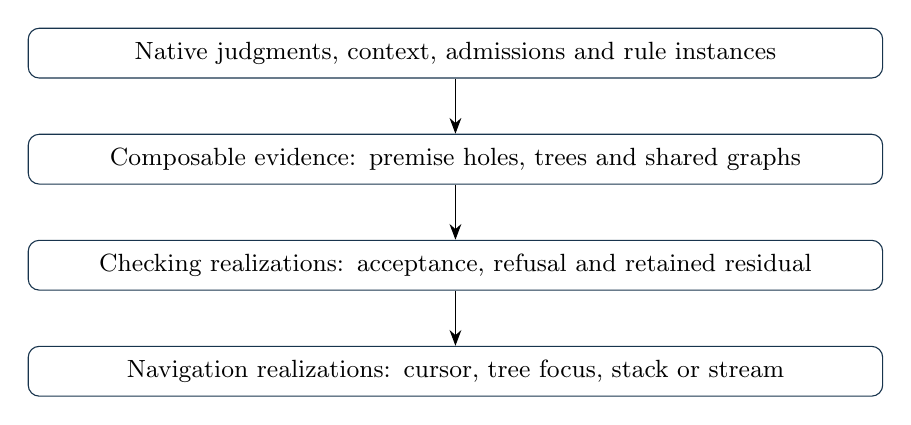
\begin{tikzpicture}[box/.style={draw=ink,rounded corners,align=center,
  text width=105mm,inner sep=5pt,font=\small},node distance=7mm,
  >={Stealth[length=2mm]}]
\node[box] (rules) {Native judgments, context, admissions and rule instances};
\node[box,below=of rules] (proofs) {Composable evidence: premise holes, trees and shared graphs};
\node[box,below=of proofs] (machine) {Checking realizations: acceptance, refusal and retained residual};
\node[box,below=of machine] (storage) {Navigation realizations: cursor, tree focus, stack or stream};
\draw[->] (rules) -- (proofs);
\draw[->] (proofs) -- (machine);
\draw[->] (machine) -- (storage);
\end{tikzpicture}
\end{center}

These are dependency levels, not successive authorities. A cursor's current
focus can be made observable, like a reader's position in a proof, but a
source calculus need not contain that position. Conversely a language that
makes scheduling or resource ownership observable needs a realization theorem
preserving precisely those observations. The model should follow those
semantics rather than the convenience of a particular storage backend.

\section{Scope and relation to the abstract-machine notes}\label{sec:scope}

The companion notes \emph{Abstract Machines} (Section~13, ``Proof machines:
scoped, licensed composition'') describe how source judgments, composable
evidence, checking realizations and navigation adapters are layered, and which
checking machines realize which kernels. This note does not repeat that
material. It supplies the mathematical structure of the evidence layer: what
composition of derivations is, how translations act on it, what costs are
attached to it, and how atomic multi-premise execution relates to it.

Section map.
\begin{center}\small
\begin{tabularx}{\linewidth}{lX}
\toprule
Section & Content \\
\midrule
\ref{sec:grounding} & Circular specifications, finite evidence and semantic partiality \\
\ref{sec:ladder} & The checking ladder and its distinct comparison axes \\
\ref{sec:free} & Rule signatures, open derivations and freeness \\
\ref{sec:kernels} & Kernels as free multicategories: trees, graphs and authored calculi \\
\ref{sec:translations} & Translations as multifunctors \\
\ref{sec:costs} & Costs: logical work, sharing (SHARE) and extension (EXTEND) \\
\ref{sec:execution} & Atomic multi-pattern steps and schedules \\
\ref{sec:revalidation} & Admission and revalidation of retained evidence \\
\ref{sec:modules} & Module coverage and the LRAT action adapter \\
\ref{sec:headline} & The costed HOL Light to MM0 translation \\
\ref{sec:dependent} & Dependent judgments, theorem authority and set models \\
\ref{sec:ledger} & Status ledger \\
\ref{sec:open} & Open problems \\
\bottomrule
\end{tabularx}
\end{center}

\section{Circular specifications and finite evidence}\label{sec:grounding}

Circular syntax and circular justification are different. A finite collection
of named propositions can contain a reference cycle, while a particular
justification for one of its conclusions is still a finite, well-founded
tree. For example, if a grounded fact $G$ is true, then $L\lor G$ is true in
strong Kleene semantics even when $L$ refers negatively to itself. The
evidence uses $G$; it does not need a proof of $L$.

Let each judgment $j:J$ have a specification $\mathsf{spec}(j)$ built from base
facts, truth references, negation, conjunction and disjunction. A valuation
is a pair $(H,F)$ of positive and negative extensions, ordered by inclusion
in both coordinates. Strong Kleene evaluation induces a monotone jump
$\Phi(H,F)$. Starting with $(\varnothing,\varnothing)$ selects its least fixed
point $(H_*,F_*)$\cite{KripkeTruth}. With consistent base facts the two
extensions are disjoint. They need not cover $J$.

The liar $L=\neg\mathsf{truth}(L)$ receives neither polarity. The truth-teller
$U=\mathsf{truth}(U)$ also receives neither in the least fixed point, although
other fixed points can make it true or false. Merely checking that an offered
valuation is a fixed point therefore does not establish groundedness.

\begin{theorem}[Grounded evidence as a native proof profile]
For the existing strong Kleene specification system with decidable base
admission and decidable equality of judgment and base labels, ten local rule
codes give an exact rule-witness interface. A
judgment $j$ has a positive or negative grounded verdict exactly when there
exists an accepted finite certificate for its specification at that polarity.
Equivalently, that signed specification has a closed proof in the free
multicategory of the interface. These statements do not require $J$ finite.
\end{theorem}
\lean{KripkeTruth.Checking.interface, Checking.check_sound, Checking.coverage, Checking.judgment_coverage, Checking.closed_proof_iff_grounded}

The local rules are the source evidence constructors: admitted positive and
negative base leaves; explicit unfolding at a truth reference; polarity reversal
at negation; two positive premises for conjunction and either negative premise
to refute it; either positive premise for disjunction and two negative premises
to refute it. There is no rule that establishes a judgment merely by citing its
own label. Generic tree and graph checking apply without a new account of
proof composition. This is one particular partial-truth logic hosted by the
framework, not a change of every kernel to a three-valued object logic.

\begin{theorem}[Finite decision agrees with the certificate authority]
Under these assumptions, if $J$ is finite, iteration from the empty valuation reaches $(H_*,F_*)$ after
at most $2|J|$ jumps. The implemented Boolean-pair iteration returns a polarity
exactly when some finite certificate for that polarity is accepted.
\end{theorem}
\lean{KripkeTruth.System.stage_eq_least, System.groundedDecide_spec, Checking.finite_decision_iff_certificate}

The bound counts semantic jumps. It neither makes a jump constant time nor
proves that the current recursive evaluator avoids repeated work. It depends
on a finite judgment domain and decidable base admission. It is not a bound for
an unrestricted self-referential truth language with quantifiers.

\begin{example}[Completion is not bivalence]
The finite example computes the twice-ascribed fact as positive, a conjunction
with a grounded false component as negative, and the liar and truth-teller as
undetermined. The completed liar computation is not unfinished work. Conversely
the initially unknown fact becomes true at a later stage, so an intermediate
unknown value does not establish ungroundedness. The fact certificate with a
forged negative claim is refused, and a self-reference with no supplied premise
is refused. The liar has no finite certificate for either polarity.
\end{example}
\lean{KripkeTruth.Example.decided_verdicts, Checking.Controls.fact_accepts, Checking.Controls.forged_false_refuses, Checking.Controls.absent_premise_refuses, Checking.Controls.false_base_leaf_refuses, Checking.Controls.cyclic_graph_refuses, Checking.Controls.liar_has_no_certificate}

\subsection{Several meanings of an absent answer}

\begin{center}\small
\begin{tabularx}{\linewidth}{@{}>{\raggedright\arraybackslash}p{0.26\linewidth}X@{}}
\toprule
Outcome & What has been established \\
\midrule
Accepted certificate & This evidence checks for this claim under these admissions. \\
Refused certificate & This candidate fails checking; another candidate may prove the claim. \\
Negative evidence & A stated negative judgment, or an obstruction under the selected authority. \\
Grounded undetermined & Neither polarity belongs to the selected least fixed point. \\
Unfinished check & A retained residual remains; no final verdict follows. \\
Outside an effective profile & The selected checking method has no authority for this request. \\
Conflicting reports & A knowledge store has both supports; the chosen logic must specify their consequence. \\
\bottomrule
\end{tabularx}
\end{center}

The shared authority algebra already distinguishes evidence, obstruction,
fragment boundaries and restartable resource frontiers. The partial-truth
profile gives one mathematically stable meaning to a boundary. It must not
turn a timeout, a missing proof or an untrusted report into a falsehood.
Nor should the three-valued semantic result replace the richer execution
status. Both coordinates can be retained.
\lean{KripkeTruth.Checking.finite_undetermined_iff_no_certificates}

\subsection{Reflection, observation and open-endedness}

Self-reference imposes a precise local obstruction: when the liar equation is
required, no total Boolean fixed-point valuation satisfies the system. This
is not a theorem that every language containing a truth symbol is inconsistent.
Gödel incompleteness is a different obstruction: an appropriate consistent,
effective arithmetical theory cannot capture every truth of its intended
standard model. Reflection levels record which theory a claim concerns;
they do not grant an unqualified rule asserting the current theory's own
soundness. The existing consistency-tower results are parameterized by their
arithmetical hypotheses, which must be instantiated before a concrete base
theory is claimed.

Model observations have their own limitations. Indistinguishability by the
selected formulas is weaker than isomorphism; downward Lowenheim--Skolem
requires the relevant language and parameter cardinal bounds. First-order
theories can be categorical at a specified infinite cardinal, so the
finite-model observation cannot be generalized to prohibit such categoricity.
These model-theoretic qualifications do not alter the local rule checker.

Neither hypersets nor a terminal coalgebra are required for the evidence
profile above. A final coalgebra is final for a specified functor in a
specified category, not an automatic universe containing every possible
logic. Likewise, observer-relative indistinguishability does not justify
substitution in arbitrary contexts: a replacement theorem must establish the
congruence or naturality law for the contexts actually permitted.

\section{The checking ladder}\label{sec:ladder}

Tier zero names a checking discipline: supply finite evidence for licensed
rule applications, with explicit dependencies and enough local choices for a
terminating checker. It does not name a weakest axiom system, a unique primitive
basis, a universal notion of truth, or a promise of polynomial checking for
every possible encoding. A powerful set theory and a modest rewrite calculus
can both have this discipline.

\begin{center}\small
\begin{tabularx}{\linewidth}{@{}>{\raggedright\arraybackslash}p{0.25\linewidth}>{\raggedright\arraybackslash}X>{\raggedright\arraybackslash}X@{}}
\toprule
Presentation & Supplied evidence & Principal checking obligation \\
\midrule
Explicit rule replay & Rule instances, premises, substitutions and side witnesses & Replay each licensed composition. \\
Retained sharing & A dependency graph and selected root & Validate references and local instances without unfolding shared premises. \\
Compressed computation & A strategy, fuel and optional checkpoints & Reproduce the specified computation and its endpoint. \\
Theory extension & Declarations, definitions and admission evidence & State conservativity or new assumptions and revalidate reuse. \\
Reconstruction & Untrusted tactic or prover output & Produce a certificate that the destination independently checks. \\
\bottomrule
\end{tabularx}
\end{center}

This is a family of comparisons rather than one total ordering. Logical
strength, source expressiveness, certificate size, checking time, search power
and trusted implementation are separate axes. A proof-size translation does
not by itself prove a runtime bound. A faithful map on existing proofs need
not reflect the existence of proofs in its target. The intuitionistic-to-classical
inclusion below is a concrete example.

Fuel illustrates both the benefit and the price of compression. If a specified
machine accepts after $n$ reduction steps, supplying $n$ makes bounded replay
decidable and reproduces that successful run. A binary count needs only
logarithmically many bits, but replay can still take $n$ steps. Checkpoints
need justification between them; an explicit trace writes more information.
A trace's linear number of local checks is not automatically linear bit-time
if those local checks manipulate large substitutions or expressions.

The library already formalizes fuelled conversion evidence, explicit equality
recipes and reproducible strategy hints. It also keeps the Lean4Lean
algorithmic checker separate from ideal typing and conversion. More fuel
recovers a successful finite run; it cannot make an incomplete algorithm
complete for a larger ideal relation. The present executable Lean-related
instance is a specified head-conversion profile, not a proof that the full
Lean kernel has been reconstructed. The Lean4Less boundary records this
distinction rather than treating implementation heartbeats as portable
reduction counts.

The comparison target matters more than the implementation language. McTT
proves soundness and completeness of an extracted checker for its specified
Martin-Lof type theory\cite{McTT}. The observational theory $\mathsf{TT}_{obs}$
has a normalizing reduction and decidable conversion and type checking for its
own rules\cite{TTobs}. These are useful reference profiles; neither result is
a completeness theorem for Lean's different judgment, nor does implementing a
checker in Rocq identify its object theory with Rocq's full calculus. Runtime
efficiency requires a separate measurement.

\subsection{Weighted answers, effects and paid work}

A useful companion model of an effectful computation is
\[
 \mathsf{Spec}(K,C,W,X)
   = W\longrightarrow\mathsf{Ans}_K(X\times W\times C),
 \qquad \mathsf{Ans}_K(Y)=Y\to_{\mathrm{fin}}K.
\]
Here $K$ is a commutative semiring of answer annotations, $C$ a commutative
monoid of branch costs, and $W$ a world or space. Sequencing combines weights,
threads each branch's state and accumulates its cost. This supplies one lawful
model, not a complete semantics of every language that returns several answers.
Reads and writes need not commute. A weight is not automatically a probability,
a degree of truth or an unresolved scheduler choice. In particular the existing
no-distributive-law result concerns probability distributions over finite sets
with specified naturality and unit laws; it is not a prohibition on every
combination of probabilistic and nondeterministic operations.
\lean{LayerEffects.Spec.bind_assoc, LayerEffects.Controls.put_get_not_comm, NondeterminismProbability.no_distributiveLaw}

Two proved information-loss boundaries matter for inference. Charging a branch
and then failing leaves no successful answer carrying that charge; the total
paid work cannot in general be recovered from the surviving answers. It needs
an execution account with its own observation contract. Likewise marginal
positive/negative counts for $A$ and $B$ do not determine counts for $A\land B$
on the same worlds. Cartesian pairing of sample bags has a lawful product,
but that product does not recover unknown dependence. A proof checker can
validate either stated calculation without silently equating their meanings.
\lean{LayerEffects.Spec.no_failed_cost_recovery, EvidenceSpaces.no_same_world_conjunction_from_marginals}

These models belong downstream of the rule and evidence layer. A categorical
completion such as $\operatorname{Ind}(\mathcal C)$, or a dependent type theory,
requires its own objects, judgments and comparison theorems; neither follows
from the displayed computation type alone. Similarly, a checked absence
frontier proves a negative claim relative to its licensed future relation.
Identifying that claim with a guest logic's internal negation requires a
separate interpretation theorem.

\subsection{Three faces across the ladder}

The operational, retained-proof and semantic faces persist across the ladder.
An execution explains how checking proceeded, a proof records what licensed
the claim, and a semantic map explains what the claim means. A compiler or
optimization must name which face it preserves, which it reflects and what
information its observation forgets.

\begin{center}
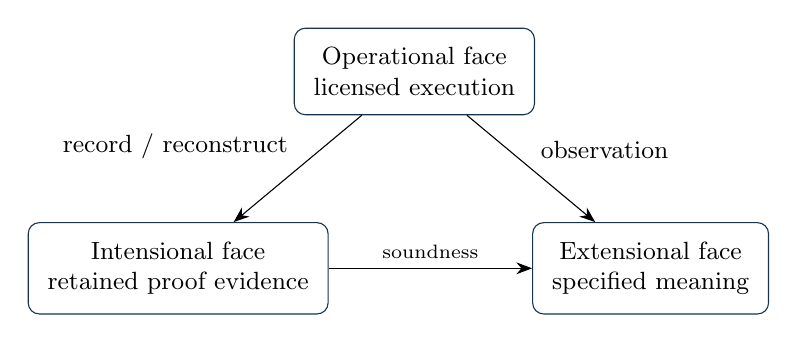
\begin{tikzpicture}[every node/.style={align=center,font=\small},
  >={Stealth[length=2mm]}]
\node[draw=ink,rounded corners,inner sep=7pt] (op) at (0,2.5)
  {Operational face\\licensed execution};
\node[draw=ink,rounded corners,inner sep=7pt] (proof) at (-3,0)
  {Intensional face\\retained proof evidence};
\node[draw=ink,rounded corners,inner sep=7pt] (meaning) at (3,0)
  {Extensional face\\specified meaning};
\draw[->] (op) -- node[above left] {record / reconstruct} (proof);
\draw[->] (proof) -- node[above,font=\scriptsize] {soundness} (meaning);
\draw[->] (op) -- node[above right] {observation} (meaning);
\end{tikzpicture}
\end{center}

For HOL, one extensional judgment is a \emph{semantic sequent}
$\Gamma\models_M A$: every admissible assignment in model $M$ satisfying the
assumptions in $\Gamma$ satisfies $A$. A Henkin model specifies the domains of
quantification, including which function values are available. Soundness
connects proof rules to this satisfaction relation; it does not identify the
model with the proof's syntax. Different proofs and execution orders can have
one semantic sequent. The arrows in the diagram require their stated
contracts and generally cannot be inverted.

\section{Rule signatures and the free cartesian multicategory}\label{sec:free}

\begin{definition}[Cartesian multicategory]
A cartesian multicategory over a type of sorts $\Sigma$ assigns to each finite
context $\Gamma : \mathrm{Fin}\,n \to \Sigma$ and sort $b$ a type
$\mathrm{Hom}(\Gamma; b)$, with variables $\mathrm{var}_i : \mathrm{Hom}(\Gamma;\Gamma_i)$
and simultaneous substitution
$\subst : \mathrm{Hom}(\Gamma;b) \times \prod_i \mathrm{Hom}(\Delta;\Gamma_i) \to \mathrm{Hom}(\Delta;b)$,
satisfying $\mathrm{var}_i[\sigma] = \sigma_i$, $t[\mathrm{var}] = t$ and
$t[\sigma][\tau] = t[\sigma[\tau]]$. A multifunctor over a map of sorts
$f : \Sigma \to \Sigma'$ sends $\mathrm{Hom}(\Gamma;b)$ to
$\mathrm{Hom}(f\circ\Gamma; f b)$, preserving variables and substitution.
\end{definition}
\lean{CartesianMulticategory, CartesianMulticategory.Functor}

Reindexing contexts by composition makes multifunctors compose without
transport; the list-indexed \name{MultiSortedClone} is the restriction to
contexts of the form $\ell.\mathrm{get}$. This is the many-sorted abstract clone
presentation; for the correspondence between clones, cartesian multicategories
and their internal languages see Saville, \emph{Clones, closed categories, and
combinatory logic}\cite{Saville}, which also recalls the multicategories introduced by Lambek
in \emph{Deductive systems and categories II}\cite{Lambek}. Lambek and Scott,
\emph{Introduction to Higher Order Categorical Logic}, treat the unary
deductive systems from which this generalizes.

\begin{proposition}[Multifunctors form a category]
Identity and composition of multifunctors satisfy the unit and associativity
laws. A multifunctor carries closed multimorphisms to closed multimorphisms.
\end{proposition}
\lean{CartesianMulticategory.Functor.id_comp, comp_id, comp_assoc, Functor.inhabited}

\begin{definition}[Rule signature, open derivations]
A rule signature $S$ assigns to each premise list $p_1\cdots p_k$ and conclusion
$c$ a type $S(p;c)$ of rule instances. Open derivations $\Term_S(\Gamma;b)$ are
generated by premise holes $\mathrm{var}_i$ and nodes
$r(t_1,\dots,t_k)$ with $r \in S(p;c)$ and $t_j \in \Term_S(\Gamma;p_j)$.
Substitution plugs derivations into holes. The generator of $r$ is
$\mathrm{gen}(r) = r(\mathrm{var}_1,\dots,\mathrm{var}_k)$.
\end{definition}
\lean{RuleSignature, RuleSignature.Term, Term.subst, RuleSignature.free, RuleSignature.gen}

\begin{theorem}[Freeness]\label{thm:free}
Open derivations with substitution form a cartesian multicategory $\Free(S)$.
For every cartesian multicategory $M$ and map of sorts $f$, restriction to
generators is an equivalence between multifunctors $\Free(S) \to M$ over $f$
and interpretations
\[ \textstyle\prod_{p,c}\; S(p;c) \longrightarrow \mathrm{Hom}_M(f\circ p;\, f c). \]
\end{theorem}
\lean{RuleSignature.universal, RuleSignature.functor_eq_of_gen, RuleSignature.lift_gen, Term.lift_subst}

\begin{theorem}[Derivability]
A sort is derivable in $\Free(S)$, i.e.\ has a closed derivation, exactly when
it lies in the inductive closure of the rule predicate $\exists r \in S(p;c)$.
Every multifunctor between free multicategories preserves derivability.
\end{theorem}
\lean{RuleSignature.derivable_iff_derives, RuleSignature.Derivable.map}

\begin{proposition}[Structural rules]
Holes may be discarded or reused, so $\Free(S)$ is cartesian; two holes of the
same sort remain distinct derivations. Generators are planar (each premise used
once, in order), and every closed derivation is planar.
\end{proposition}
\lean{Term.duplicate_holes_distinct, Term.gen_linear, Term.closed_linear}

Here the holes are metalevel proof dependencies for the fixed rule signature.
This construction does not authorize copying an object-level linear resource
or a capability. Such constraints must already be present in the judgment,
the allowed instances or a resource-sensitive composition. Planarity of these
closed terms is not an equivalence of arbitrary linear, symmetric and
cartesian object logics.

\begin{theorem}[Schematic level: instance actions]
If a map of sorts carries every rule instance to an instance of the mapped
premises and conclusion, it induces a multifunctor $\Free(S) \to \Free(S)$, and
derivability is closed under the map. Actions compose coherently: if two
actions compose on sorts and on instances to a third, acting by the two in turn
agrees with acting by the third on every derivation, up to the identification of
sorts. In particular substitution of formulas for atoms acts on the
intuitionistic and classical Hilbert multicategories, coherently with
composition of substitutions, so Hilbert derivability is substitution closed as
a consequence of freeness.
\end{theorem}
\lean{RuleSignature.InstanceAction, RuleSignature.actFunctor, RuleSignature.Derivable.act, RuleSignature.act_comp_heq, Hilbert.substFunctor, Hilbert.substFunctor_comp_heq, Hilbert.source_subst}

\begin{remark}[Contexts, binders and side conditions]
Object-level contexts and binders are part of the sorts: a HOL Light theorem
carries its hypothesis set and its terms their binders, and side conditions
such as freshness for abstraction are part of the rule-instance predicate. They
change the generators, not the kind of structure (Section~\ref{sec:kernels}).
Rules with one conclusion give a multicategory; multi-product consuming steps
are treated in Section~\ref{sec:execution}.
\end{remark}

\section{Kernels as free multicategories}\label{sec:kernels}

A kernel with a decidable rule-instance interface
$(\mathrm{W}, \mathrm{isInstance})$ presents the signature whose rule instances
are accepted witnesses.

\begin{theorem}[Derivability]
Kernel derivability coincides with closed derivability in the free
multicategory on the kernel's accepted witnesses.
\end{theorem}
\lean{RuleWitness.signature, RuleWitness.derivable_iff_derives}

\begin{theorem}[Certificate trees are closed morphisms]
For every conclusion $b$, closed derivations of $b$ correspond bijectively to
certificate trees of the kernel that its tree checker accepts with conclusion
$b$. Erasure to trees is injective.
\end{theorem}
\lean{RuleWitness.closedEquiv, RuleWitness.toDerivation_injective}

\begin{theorem}[Graphs unfold]
Replaying a shared derivation graph with the unfolding step yields exactly the
judgments of ordinary replay, now with closed derivations. Every node of an
accepted graph denotes a closed morphism of its conclusion, and therefore an
accepted certificate tree.
\end{theorem}
\lean{RuleWitness.termStep, RuleWitness.unfold_judgments, RuleWitness.unfold_root, RuleWitness.unfold_tree}

\begin{theorem}[Graphs present exactly the closed morphisms]
Every closed derivation is the unfolding of the last node of some accepted
derivation graph. With the previous theorem, accepted graphs present exactly
the closed morphisms of the free multicategory: sharing is a property of the
representation, never of the morphism.
\end{theorem}
\lean{RuleWitness.presented, RuleWitness.presented_block, DerivationGraph.replayWith_relocate, DerivationGraph.replayWith_append}

\begin{theorem}[Authored calculi]
For every validated authored calculus, the existing open derivations with
ordered premise contexts are exactly the terms of the free multicategory on its
rule applications, and plugging derivation vectors is substitution. Every
interpretation of the rule applications in a cartesian multicategory extends
uniquely to open derivations, preserving substitution. Accepted raw open proofs
decode computably to typed open derivations.
\end{theorem}
\lean{CertificateGSLT.ruleSignature, OpenDerivation.termEquiv, OpenDerivation.toTerm_bind, interpret_bind, interpret_unique, decodeOpen}

\begin{corollary}
The classifying category of every authored calculus (VibeITP, projected
Metamath snapshots, HOL Light's first-order calculus) is the category of
contexts of a free cartesian multicategory, with products by concatenation.
\end{corollary}
\lean{ClassifyingContext.instCategory, ClassifyingContext.concatIsLimit, OpenDerivation.termEquiv}

\begin{center}\small
\begin{tabularx}{\linewidth}{>{\raggedright\arraybackslash}p{0.27\linewidth}>{\raggedright\arraybackslash}X>{\raggedright\arraybackslash}p{0.33\linewidth}}
\toprule
Kernel & Rule-instance interface & Free multicategory \\
\midrule
Intuitionistic / classical Hilbert & finite codes, profile-gated excluded middle & \name{RuleWitness.signature (interface p)} \\
Extended Hilbert & classical codes and admitted definitions & \name{RuleWitness.signature (interface hs)} \\
HOL Light & ten rules and policy axioms & \name{RuleWitness.signature (ruleWitness policy)} \\
LRAT, RUP fragment & input clauses and RUP instances & \name{RuleWitness.signature (interface F)} \\
Authored calculi & rule applications & \name{CertificateGSLT.ruleSignature} \\
Grounded circular truth & ten codes over signed specifications & \name{RuleWitness.signature (Checking.interface system)} \\
Guarded atom rules, presentations & original rule codes & \name{Presentation.ruleWitness} \\
\bottomrule
\end{tabularx}
\end{center}

\section{Translations as multifunctors}\label{sec:translations}

By Theorem~\ref{thm:free}, a translation is determined by the images of rule
instances; derivability is preserved automatically.

\begin{theorem}[Faithful renamings]
A sort-preserving renaming of rule instances that is injective induces an
injective multifunctor.
\end{theorem}
\lean{RuleSignature.rename, RuleSignature.lift_rename_injective}

\begin{theorem}[Intuitionistic into classical]
The inclusion of intuitionistic into classical Hilbert rule instances induces a
faithful multifunctor that preserves but does not reflect derivability:
excluded middle is classically derivable and not intuitionistically derivable.
\end{theorem}
\lean{Hilbert.inclusion, Hilbert.inclusion_faithful, Hilbert.inclusion_not_reflecting}

\begin{theorem}[Classical into extended]
For every list of definitions, the inclusion of classical into extended rule
instances induces a faithful multifunctor. For admitted fresh definitions it is
conservative on claims in the old vocabulary. It is not full: citing a
definition is a derivation in the image of no classical derivation.
\end{theorem}
\lean{Extension.inclusion, Extension.inclusion_faithful, Extension.inclusion_conservative, Extension.inclusion_not_full}

\begin{theorem}[HOL Light into its first-order calculus]
Each accepted HOL Light rule instance is translated by the node step on its
canonical premise context and decoded to a typed open derivation of its rendered
conclusion. This determines a unique multifunctor from HOL Light's free rule
multicategory to the free multicategory of its first-order calculus over the
rendering of theorems. It preserves derivability, and for admitted axiom lists
reflects it: the calculus derives the rendering of a sequent exactly when HOL
Light derives a theorem with that sequent. Positive control: $\vdash p = p$ by
\textsf{REFL}; negative control: $\vdash \mathsf{F}$.
\end{theorem}
\lean{HOLLight.FirstOrder.generatorImage, translation, translation_unique, translation_derivable, translation_reflects, Kernel.reflexivity_translated, Kernel.falsity_not_translated}

\begin{theorem}[Sharing commutes with translation]
For any interpretation of a kernel's rule instances in a free multicategory,
translate a shared derivation graph node by node: check each node against its
source premise sorts and instantiate its rule image with the translated
premises. From translated entries this computes exactly the multifunctor images
of the unfolded entries. Hence every accepted graph translates with one rule
image per node, and the value at each node is the multifunctor image of that
node's closed derivation. In particular this holds for HOL Light graphs and the
translation above.
\end{theorem}
\lean{RuleWitness.liftStep, RuleWitness.liftStep_liftEntry, RuleWitness.replay_liftStep, RuleWitness.shared_translation, HOLLight.FirstOrder.shared_translation}

\begin{remark}
The existing compilation of first-order calculi into MM0 (the system of
\emph{Metamath Zero: The Cartesian Theorem Prover}\cite{Carneiro}) and the existing proof-graph
translation with shared lemmas complete the chain to MM0 at the level of
certificates. That existing translation builds each lemma with the same node
step over the cumulative context. On all 25 nodes of the three real HOL Light
exports of Section~\ref{sec:headline}, each of its lemmas coincides with the raw
rule proof from which the multifunctor's rule image is decoded, after renaming
premise positions to the lemma's parents. This is an executed comparison; the
general equality is open (Section~\ref{sec:open}).
\end{remark}

\section{Costs: logical work, sharing and extension}\label{sec:costs}

\begin{theorem}[Additivity]
Rule nodes are additive under substitution, each hole occurrence charged once:
$\size(t[\sigma]) = \size(t) + \sum_{i \in \occ(t)} \size(\sigma_i)$.
\end{theorem}
\lean{Term.size_subst}

\begin{theorem}[Affine translations are linear on trees]
If every rule image uses each premise at most once and has at most $c$ rule
nodes, the induced multifunctor satisfies $\size(F t) \le c \cdot \size(t)$.
\end{theorem}
\lean{RuleSignature.lift_size_le}

\begin{theorem}[SHARE: a contraction-induced expansion gap]
Translate the chain calculus (one premise per step) into the duplication
calculus by an image citing its premise twice. The $k$-chain has $k+1$ nodes;
its translation is a tree with $2^{k+1}-1$ nodes; the duplication calculus has
an accepted shared graph with $k+1$ rows for the same conclusion. The
contracting image is not affine.
\end{theorem}
\lean{Contraction.contraction_gap, Contraction.image_not_affine, ProofSharingBounds.no_tree_sizeSimulation_dag}

\begin{remark}[EXTEND]
Extension by definitions changes the multicategory: the inclusion is faithful
and conservative but not full (Section~\ref{sec:translations}), and literal
expansion of an admitted doubling chain has $2^{k+1}-1$ formula nodes from
encoded size at most $5(k+1)(k+2)$ (\name{PropositionalExtension.literal_expansion_gap}).
Sharing never changes the multicategory: a graph and its unfolded tree are one
morphism. In the sense of Cook and Reckhow, \emph{The Relative Efficiency of
Propositional Proof Systems}, a translation with polynomial size and time bounds
is a p-simulation. The proved size separation rules out polynomial-size
translation from the shared duplication certificates to trees; the
straightforward tree-to-DAG representation comparison has no such size
obstruction. An executed compiler-time bound must be supplied separately.
Extended resolution's polynomial
simulation of DRAT (Kiesl, Rebola-Pardo and Heule, \emph{Extended Resolution
Simulates DRAT}) is the corresponding EXTEND phenomenon for SAT certificates.
\end{remark}

\begin{proposition}[Time accounts]
The p-simulation of HOL Light proof graphs by MM0 has a degree-ten certificate
bound and a degree-ten declared time account; the declared time is at least the
weight of the lemmas the translation writes. An operational simulation derives
its clock from a finite-stack machine execution, and such clocks are positive.
\end{proposition}
\lean{HOLLight.FirstOrder.graphTranslate_weight, graphTime_ge_weight, Kernel.mm0Simulation, OperationalPSimulation.toPSimulation, OperationalPSimulation.time_positive}
\status{The HOL Light to MM0 time account is declared, bounded below by output
weight; its finite-stack realization is open.}

\section{Atomic multi-pattern steps and schedules}\label{sec:execution}

A step keeps some occurrences, consumes others and produces atoms, when its rule
admits them; this is the shape of multi-headed CHR simpagation (Di Giusto,
Gabbrielli and Meo, \emph{On the expressive power of multiple heads in CHR}) and
of chemical-style rewriting (Berry and Boudol, \emph{The Chemical Abstract
Machine}).

\begin{theorem}[Local characterization of replay]
Sequential replay with any local step accepts exactly when the final cache
extends the initial one, has one value per node, every reference points
backward, and every node's step on its looked-up premises yields its value.
\end{theorem}
\lean{DerivationGraph.replayWith, DerivationGraph.replayWith_iff_local, DerivationGraph.replayWith_judgmentStep}

\begin{theorem}[Schedule independence]
For a step that ignores physical reference positions, reordering a graph by any
permutation that keeps premises before consumers, with references relocated,
accepts exactly when the original order does (for topological originals), and
moves each node's value to its new position. A reordering that places a premise
after its consumer is refused. The numbers of local steps and premise lookups
are invariant. In particular judgment replay and unfolding are schedule
independent.
\end{theorem}
\lean{DerivationGraph.replayWith_permute, replayWith_permute_reflect, replayWith_permute_iff, replayWith_permute_refused, permute_lookups, replay_permute, RuleWitness.unfold_permute}

\begin{theorem}[Monotone steps are derivations]
Without consumption, running single-product steps is replay of the
corresponding derivation graph, and every accepted trace denotes, at every step,
a closed morphism of the free multicategory on the step rules. A monotone step
with several products runs exactly as the sequence of its single-product
components.
\end{theorem}
\lean{MultiPremiseSteps.run_monotone, run_monotone_unfolds, run_split}

\begin{theorem}[Consumption]
In an accepted trace a consumed occurrence is never cited again; occurrences
may be kept twice but not consumed twice, nor kept and consumed together. Two
steps competing for one occurrence lead to different stores, neither of which
can fire the other. Two steps with independent footprints (neither consumes what
the other cites, and the second cites no product of the first) fire in either
order, with the same live atoms up to the order of their products. In the
formalized tree of single-wire cuts, a composite has one internal wire fewer
than generators. The split/join process has two steps and two internal wires,
so that compositional syntax cannot represent it while preserving those
counts. This rules out that syntax as a complete account; it does not rule out
encoding processes in categories or alternative polycategorical frameworks.
\end{theorem}
\lean{MultiPremiseSteps.consumed_not_cited, Controls.consumption_not_confluent, Controls.keep_twice, Controls.take_twice_refused, independent_commute, Controls.independent_steps_commute, PolyComposite.wires_add_one, process_not_polycategorical}

\begin{remark}[What the correspondence keeps]
Kept: rule witnesses, ordered and repeated premise occurrences, every
conclusion, acceptance including refusal of unused bad steps, and step counts.
Forgotten: the order of independent steps; sharing (a graph and its unfolding
are one morphism); the identity of steps not used by the selected root.
Consumption keeps resources linear and needs monoidal composition of
processes; negative reads are outside this step shape.
\end{remark}

\section{Admission and revalidation of retained evidence}\label{sec:revalidation}

\begin{theorem}[Exact revalidation]
For a graph accepted under one interface, rechecking each node's rule instance
against another interface, with premises read from the retained cache, succeeds
exactly when the mapped graph replays under the new interface to the same
cache. Admitted extensions (witness maps keeping accepted instances accepted)
transport evidence; checked judgments are reusable in larger rule systems; a
retained source-address schedule replays to the identical state under a new
interface accepting each instance it used.
\end{theorem}
\lean{DerivationGraph.revalidate_iff, replay_extend, CheckedJudgment.extend, BorrowedCursor.run_reinterpret}

\begin{theorem}[Propositional admission joined to retained evidence]
Every accepted intuitionistic graph is accepted classically with the same cache.
An accepted extended graph remains accepted when further admitted definitions are
appended. Classical evidence for excluded middle is refused on intuitionistic
revalidation; evidence citing a definition that was replaced by a different
admitted definition is refused.
\end{theorem}
\lean{Revalidation.intuitionistic_to_classical, Revalidation.checkDAG_append, Controls.em_refused_intuitionistically, Controls.worked_extended, Controls.worked_changed_refused}

\section{Module coverage and the LRAT action adapter}\label{sec:modules}

\begin{theorem}[HOL Light kernel module]
The first-order calculus of HOL Light over an axiom list renders as a portable
module that the verified reader and the original validator load exactly. The
loaded package derives the rendering of a sequent exactly when HOL Light derives
a theorem with that sequent, for admitted axiom lists.
\end{theorem}
\lean{HOLLight.FirstOrder.kernelModule, kernelModule_read, kernelModule_faithful}
\status{Exported for the bare kernel: 147 rules, 991\,249 bytes, read back through
the actual reader and validator.}

\begin{theorem}[LRAT actions]
A reverse-unit-propagation addition is a multi-premise rule instance whose
premises are its hinted clauses, and it is sound. An LRAT action stream compiles,
with identifiers resolved to positions and deletions enforced, to a derivation
graph; acceptance of that graph with an empty clause refutes the formula, and
every action denotes a closed morphism of the free multicategory on RUP
instances. A resolution-asymmetric addition need not be implied, so it is not a
rule instance of this calculus.
\end{theorem}
\lean{PropositionalLRATActions.rupCheck_sound, check_sound, check_graph, check_unfolds, rat_not_implied, rat_not_rule_instance}

\begin{center}\small
\begin{tabularx}{\linewidth}{>{\raggedright\arraybackslash}p{0.24\linewidth}>{\raggedright\arraybackslash}X>{\raggedright\arraybackslash}p{0.24\linewidth}}
\toprule
Native profile & Faithful presentation & Portable module \\
\midrule
VibeITP & authored calculus, \name{kernel_derives_iff_classifyingArrow} & yes, 123 schemas \\
Metamath snapshot & projected authored calculus & yes, 25 schemas \\
HOL Light kernel & first-order calculus, \name{kernelModule_faithful} & yes, 147 rules \\
Hilbert, extended Hilbert & exact rule codes; sorted Hilbert source presentation also exists & not qualified here \\
LRAT (RUP fragment) & action calculus, \name{check_sound} & no (RUP is a computed check) \\
Grounded circular truth & signed evidence rules, \name{judgment_coverage} & no (base admission is a parameter) \\
MM0, Megalodon & owned by the active MM0 lane & not covered here \\
Rho, MeTTa equations, GSLT recipes & retained workers (\emph{Abstract Machines}, Section~13) & open \\
\bottomrule
\end{tabularx}
\end{center}

\section{The costed HOL Light to MM0 translation}\label{sec:headline}

The existing receiver replays real HOL Light exports, lowers the registered
receipts to proof graphs, translates each node through its first-order step,
compiles the shared lemmas to MM0 saved proofs, checks them in Lean and prints
specification and proof texts. The reference MM0 tools then compile the proof
text and verify the binary against the specification.

\begin{center}\small
\begin{tabular}{@{}lrrrrrrr@{}}
\toprule
Export & events & spec & MMU & emit & MMB & compile & verify \\
 & & (MB) & (MB) & (s) & (bytes) & (s) & (s) \\
\midrule
\textsf{T\_DEF} & 1 & 26.2 & 40.1 & 14.4 & 220\,512 & 0.58 & 0.13 \\
\textsf{TRUTH} & 8 & 22.6 & 252.2 & 2166 & 223\,536 & 4.08 & 0.14 \\
\bottomrule
\end{tabular}
\end{center}

Emission includes the Lean-side check and printing of each text: for
\textsf{TRUTH}, lowering, node translation and shared-proof compilation take
under a minute, while checking and printing the proof text and the MM1 text take
16 and 19 minutes at a peak of 2.8\,GiB. The specification encodes the fixed
147-rule presentation and dominates the binary certificate; the eight-node
proof adds about three kilobytes to it. The
proved bounds are polynomial of degree ten with generous constants; the measured
growth is far below them. The text formats and the in-process checking dominate
wall-clock cost, not the reference verifier. These are executed times of the
existing binary and are kept separate from the logical work and the declared
time account of Section~\ref{sec:costs}, which the following table reports in
the measures of the proved bounds (graph size $N$, lemma-certificate weight,
first-order rule nodes and declared time).

\begin{center}\small
\begin{tabular}{@{}lrrrrr@{}}
\toprule
Export & nodes & $N$ & certificate weight & rule nodes & declared time \\
\midrule
\textsf{T\_DEF} & 1 & 371\,826 & 185\,913 & 1 & $1.9\times10^{22}$ \\
\textsf{TRUTH} & 8 & 3\,610\,421 & 4\,562\,433 & 1\,505 & $1.3\times10^{24}$ \\
core \textsf{bool} & 16 & 43\,070\,295 & 24\,292\,374 & 1\,513 & $5.2\times10^{28}$ \\
\bottomrule
\end{tabular}
\end{center}

These measurements are historical qualification runs of the receiver frozen
on 13 October 2026. They have not been reproduced with a rebuilt receiver in
the present source state and are not current performance guarantees.

The certificate weight is $1.26\,N$ on \textsf{TRUTH}, while the proved bound
$(35\cdot10^{12}+2)(N+1)^{10}$ exceeds $10^{78}$: the degree-ten bound is
sound and very loose. The declared time is dominated by its fourth-power
comparison term and says nothing about executed time. On the sixteen-event core
\textsf{bool} export, the executed compilation to MM0 saved proofs exhausted
its available memory at the last of its sixteen nodes, after assembling a
156-rule presentation; memory, not time, bounds the executed translation there.


\section{Dependent judgments, theorem authority and set models}\label{sec:dependent}

Four independent questions determine a kernel interface. Keeping them
separate permits the same computation to support several faithful consumers.

\begin{center}\small
\begin{tabularx}{\linewidth}{@{}lX@{}}
\toprule
Coordinate & Declared contract \\
\midrule
Judgment & What follows, in which context and theory: typing, equality,
reachability, one answer, or a complete result observation. \\
Evidence & What is checked: local rule data, a tree, a shared graph, or a
finite trace of licensed transitions. \\
Authority & How checked conclusions can be constructed and used; which
profile and declaration snapshot authorize them. \\
Observation & What execution retains or exposes: verdict, pending work,
cost, dependencies, or an optional exportable history. \\
\bottomrule
\end{tabularx}\end{center}

An LCF interface protects theorem construction. It can also record proof
terms or a journal. Certificate checking can mint the same logical kind of
value without retaining the certificate. Neither choice supplies a constant
checking cost, proves a native seal implementation, or recovers evidence
that execution erased. A checked finite trace can be evidence when its
transition rules establish the intended conclusion. A trace of an unrelated
implementation is not automatically a derivation of that judgment.

The MeTTa equation kernel is sound and complete for its native reachability
judgment. Full HE or PeTTa evaluation, resource consumption and mathematical
multi-premise inference require their respective judgments. No single one
of these observations defines every useful MeTTa kernel. The design of a MeTTa kernel integrating these judgments remains open;
the following connection uses an existing mathematical calculus.

\subsection{Source queries, retained execution and checked publication}
\label{sec:interaction-queries}

The occurrence-based interaction model now connects its source grammar to
the existing retained read machine. This connection concerns execution of
queries and their resource footprints. A proof checker remains responsible
for the logical conclusion of an inference request.

\begin{center}
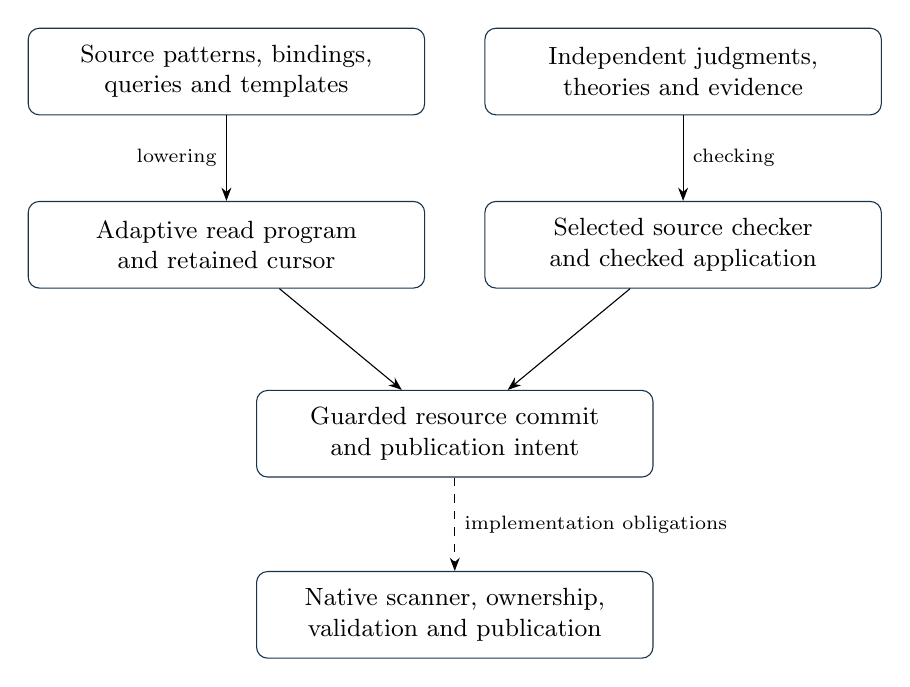
\begin{tikzpicture}[>=Stealth, node distance=7mm,
  box/.style={draw=ink,rounded corners,align=center,font=\small,
    text width=48mm,minimum height=11mm}]
\node[box] (sources) at (-29mm,0) {Source patterns, bindings,\\queries and templates};
\node[box] (judgments) at (29mm,0) {Independent judgments,\\theories and evidence};
\node[box] (queries) at (-29mm,-22mm) {Adaptive read program\\and retained cursor};
\node[box] (checker) at (29mm,-22mm) {Selected source checker\\and checked application};
\node[box] (commit) at (0,-46mm) {Guarded resource commit\\and publication intent};
\node[box] (native) at (0,-69mm) {Native scanner, ownership,\\validation and publication};
\draw[->] (sources) -- node[left,font=\scriptsize]{lowering} (queries);
\draw[->] (judgments) -- node[right,font=\scriptsize]{checking} (checker);
\draw[->] (queries) -- (commit);
\draw[->] (checker) -- (commit);
\draw[->,dashed] (commit) -- node[right,font=\scriptsize]{implementation obligations} (native);
\end{tikzpicture}
\end{center}

\begin{theorem}[Source-query lowering]
Suppose each region read returns exactly its finite occurrence family, in
the scanner's chosen order. The constructed read program for a source list
returns exactly the original compiler's row multiset after forgetting answer
order. This covers reads, takes, uniqueness, aggregation, pure computed
bindings, conjunction, nested absence and \code{every}. Matching alternatives,
duplicate-labelled occurrences and computed-result positions are retained.
The proof is by the source grammar, using the local scanner equation and
the independent read interpreter; whole-program soundness is not a premise.
\end{theorem}
\lean{Sources.Query.scanList_complete, Sources.Query.run_step, Sources.Query.run_compile}

An \code{every} query returns one amalgamated row even when its body has no
rows. Its enclosing absence is therefore false. With the established sound,
complete and minimal matcher laws and theory-respecting pure computations,
a completed empty answer is equivalent to there being no row in the
independent declarative source relation. A scanner that omits an occurrence
can fabricate emptiness and fails the explicit scanner premise.
\lean{Sources.Query.run_empty_iff_no_declarative, Sources.Query.Execution.completed_agreement, Sources.Query.Controls.vacuous_rows_are_present, Sources.Query.Controls.omitted_region_reply_is_not_complete}

\begin{theorem}[Retained source execution]
The existing cursor completes a compiled query after the number of reads on
its selected finite path plus one return inspection. Splitting the budget
preserves its entire saved packet and accumulated read charge. A paused
packet exposes no completed answer. Successful validation and resumption
against a new complete view recover that view's source rows; a changed
performed read refuses resumption and retains the old packet. These are
region-read counts, not bounds on matcher work or computed-binding evaluation.
\end{theorem}
\lean{Sources.Query.Execution.execute_complete, Sources.Query.Execution.execute_split, Sources.Query.Execution.completed_absence, Sources.Query.Execution.resumed_rows, Sources.Query.Controls.partial_query_is_not_absence, Sources.Query.Controls.changed_prefix_retains_refused_packet}

The certificate records actual adaptive reads, including empty replies.
Reordering equal-labelled occurrences preserves the row-bag observation but
changes the ordered certificate. A new acknowledgement for an unread key can
be observed after resumption, whereas changing the message that selected that
key invalidates the continuation. The source absence constructor additionally
retains its declared completeness regions, which can be stronger than the
adaptive observations needed merely to establish an empty join.
\lean{Sources.Query.validated_source_rows, Sources.Query.Controls.adaptive_dependency_is_bound, Sources.Query.Controls.absence_row_retains_full_footprint, Sources.Query.Controls.bag_agreement_does_not_validate_reordering, Sources.Query.Controls.resume_sees_unread_arrival}

A cached prefix keeps the observations it originally made. Extending it runs
only the answer-selected suffix and concatenates the two read certificates.
If the old certificate is valid in the new store, the resulting observation
equals an independent interpretation of the sequential query there. A changed
old read refuses the combined observation even when the suffix has just read
the replacement value. Thus a fresh read cannot rebase stale evidence. These
laws concern pure queries; they do not license recomputation of observable
effects hidden behind a cached result.
\lean{ReadOnlyQuery.extend_eq_run_bind_of_valid, ReadOnlyQuery.checkReads_extend, ReadOnlyQuery.changed_cached_read_refuses_extend, ReadOnlyQuery.Controls.newer_read_does_not_rebase_cached, ReadOnlyQuery.Controls.cached_then_query_retains_both}

Checked publication reads the selected source, consumes pending work and
produces evidence only after the existing open-rule checker succeeds.
Its validity theorem governs those steps from a valid initial store;
arbitrary writes and native capability confinement require their own
contracts. Inserting a refused evidence record violates the invariant.
Adding another source object while retaining the old one does not revoke
the old request: revision replacement must retire the earlier authority.
A well-sorted record alone does not establish derivability.
\lean{ProgrammableJudgmentTransforms.step_preserves_validity, ProgrammableJudgmentTransforms.stored_evidence_derivation, ProgrammableJudgmentTransforms.retaining_source_keeps_old_request_enabled, ProgrammableJudgmentTransforms.refused_evidence_write_breaks_validity, ProgrammableJudgmentServices.program_intents_preserve}

Conditional composition similarly keeps the computed guard distinct from
the net update. Intermediate freshness can remain necessary when the final
writes cancel. The proved mover condition licenses fusion of separated
commits at the declared observation; unrestricted history equality does not
follow. Both creation and removal windows have separating observers. The
conditional-rewriting literature supplies the broader overlap and condition-
transport programme\cite{BehrSobocinski,BehrKrivine}; these concrete results do
not yet enumerate symbolic occurrence-map overlaps or establish that general
categorical programme.
\lean{CommitPrecondition.sequential_holds_iff, Commit.composition_exact, OccurrenceCommits.executable_fusion_iff, OccurrenceCommits.fusion_not_traceEq}

\status{The source-query lowering and retained-cursor comparisons are checked.
The native interaction engine now retains absence and every as nested groups
of jobs. Computed sources use its existing request/resume path; a reply handle
identifies one request generation. Native controls exercise vacuous and nested
aggregation, nonlinear matching, query-local bindings, changed dependencies,
cancellation, stale replies, allocation failure and explicit post-effect
failure. Both space programming and a client invoking the actual proof checker
use that machinery. Complete scanner qualification, transitive dependencies
of arbitrary computed code, view lifetime, full backend preparation, atomic
revision validation and failure-history correspondence remain obligations.
Shared execution
does not identify Rho, equational reachability, HOL, MM0 or VibeITP judgments,
nor construct new translations between them.}

The existing correlated-reply model separately proves that a consumed or
cancelled request identity stays absent through arbitrary later operations.
Retargeting an old reply to the current request supplies a separating control:
the value reaches the wrong continuation despite there being only one live
request. The native generation check follows this contract; its memory and
seal implementation retain their qualification obligations.
\lean{Kernel.CorrelatedReplies.consumed_reply_stays_refused, Kernel.CorrelatedReplies.cancelled_reply_stays_refused, Kernel.CorrelatedReplies.Controls.stale_request_cannot_answer_next, Kernel.CorrelatedReplies.Controls.replacing_supplied_identity_accepts_wrong_reply}

The selected native checkpoint passes 404 continuation and failure controls,
including incomplete matching and refused waiter registration. Twenty
mathematics programmes, thirteen space-interaction fixtures and twenty cached-
read assertions agree across the
current-source build, generated Cesta project and plain-C export. The three
executables are byte-identical under the unchanged Cesta pin. This comparison
supplies the interpreted library tree explicitly; the C export does not yet
package those resources. Sanitizer qualification also identifies its SWI
provider: a reviewed corrected build passes, while the installed provider
retains a reproducible cleanup leak. Neither build agreement nor these finite
executions constitute a whole-runtime refinement theorem.

Computed premises preserve each dialect's value boundary. In Prime, ordinary
binding lets structural checkers inspect held source records without exposing
their carriers or executing embedded code. In PeTTa, a complete cached table
can be borrowed through a paused synchronous caller's lease under matching
source and host semantics; no active generator is shared by that admission.
Qualified controls retain the original Space reads and run cached effects
once. A separate negative lookup of a never-materialized logical location
still lacks a registry dependency and can publish a stale cached answer.
That witness remains open, alongside State and foreign-read integration;
Space certificates alone do not establish complete dependency tracking.

\subsection{An exact reason to require dependency}

The need for dependent typing can be stated without treating every richer
type theory as one system. Fix the direct Curry--Howard contract
\[
  A : \mathsf{Type},\qquad P : A \to \mathsf{Type},\qquad
  \prod_{x:A} P(x),
\]
where the indices are the same values that programs consume, rather than
codes copied into a second level. In the maintained annotated pure type
system, this context and product are well formed if and only if both the
ordinary function and value-to-type product rules are present. Neither rule
is assumed in advance. This identifies a least formation basis for this
interface, uniformly in the conversion bubble. Thus the dependent vertex
admits the contract even in the weak conversion core, while the simple,
polymorphic and type-operator vertices reject it under every conversion
policy. The actual introduction and application rules retain the same value:
given $f:\prod_{x:A}P(x)$ and $a:A$, application has type $P(a)$, with $a$
substituted directly into the evidence type.
\lean{HypercubeBubbles.directValueIndexedForall_iff_contains_dependentProducts, HypercubeBubbles.dependentProducts_least_directInterface, HypercubeBubbles.directForall_abstract, HypercubeBubbles.directForall_apply, HypercubeBubbles.directValueIndexedForall_absent_off_dependent_face}

\paragraph{A minimum relative to the requested interfaces.}
Write $F=(\ast,\ast,\ast)$ for ordinary functions,
$D=(\ast,\square,\square)$ for value-indexed type families,
$P=(\square,\ast,\ast)$ for polymorphism, and
$O=(\square,\square,\square)$ for type operators. Each triple records the
sort of the domain, codomain and resulting product. With the fixed sort
axiom $\ast:\square$, the checked formation requirements are:
\begin{center}
\begin{tabularx}{\linewidth}{@{}Xl@{}}
\toprule
Direct interface in the annotated syntax & Least product basis \\
\midrule
$A:\mathsf{Type},\ P:A\to\mathsf{Type};\ \prod_{x:A}P(x)$ & $\{F,D\}$ \\
The preceding interface, $\prod_{X:\mathsf{Type}}X\to X$,
and the kind $\mathsf{Type}\to\mathsf{Type}$ & $\{F,D,P,O\}$ \\
\bottomrule
\end{tabularx}
\end{center}
The second row is proved by constructing the three actual typing derivations
and recovering every required rule from any such derivations. Removing any
of the four rules defeats at least one requested interface, under every
bubble. The polymorphic identity also has its actual program inhabitant.
\lean{HypercubeBubbles.directFormationInterfaces_iff_contains_constructionProducts, HypercubeBubbles.constructionProducts_least_directInterfaces, HypercubeBubbles.directInterfaces_refused_of_missing_rule, HypercubeBubbles.polymorphicIdentity_typed}

\begin{center}
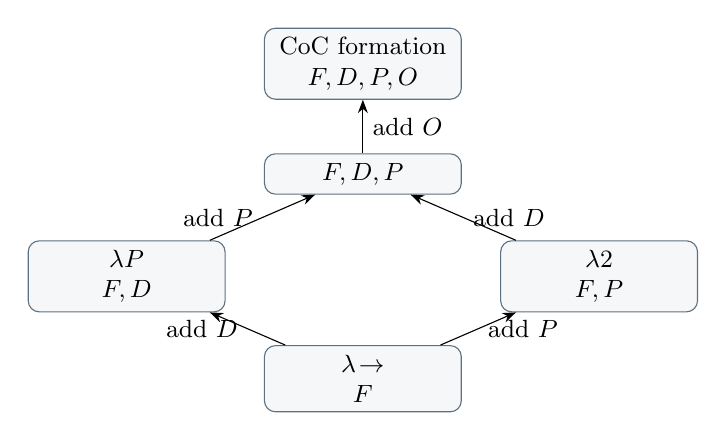
\begin{tikzpicture}[>=Stealth, every node/.style={align=center,font=\small},
  profile/.style={draw=ink!70,rounded corners,fill=ink!4,minimum width=25mm}]
\node[profile] (simple) at (0,0) {$\lambda\!\to$\\$F$};
\node[profile] (dep) at (-3,1.3) {$\lambda P$\\$F,D$};
\node[profile] (poly) at (3,1.3) {$\lambda 2$\\$F,P$};
\node[profile] (both) at (0,2.6) {$F,D,P$};
\node[profile] (coc) at (0,4) {CoC formation\\$F,D,P,O$};
\draw[->] (simple) -- node[left] {add $D$} (dep);
\draw[->] (simple) -- node[right] {add $P$} (poly);
\draw[->] (dep) -- node[left] {add $P$} (both);
\draw[->] (poly) -- node[right] {add $D$} (both);
\draw[->] (both) -- node[right] {add $O$} (coc);
\end{tikzpicture}
\end{center}
This is one projection of the profile graph: it shows product formation with
the conversion bubble held as a parameter. The four-rule endpoint is CoC's
formation profile; ordinary CoC also fixes beta conversion. An arbitrary
bubble at that endpoint need not be consistent or decidable. MLTT-like
profiles additionally state their universes, dependent pairs, identity
elimination and admitted inductive rules. Those are further branches, not
consequences of the two-rule dependency result. The cube is the classical
formation framework~\cite{BarendregtCube}; the theorem here identifies the
minimum for these particular annotated interfaces.

This is a necessity theorem for a named interface, not the claim that all
logic or verification requires dependent types. HOL can quantify with logical
constants, and singleton or two-level encodings can reify values before types
refer to them. Those encodings change the interface: a separate route must
relate a runtime value to its type-level representative. LF presents logics
through signatures and judgments-as-types~\cite{HarperHonsellPlotkin};
adequacy relates the specified object judgments to their LF evidence. The
formation minimum above is not that adequacy theorem and does not imply
that every encoding of higher-order logic requires a CoC host.

\paragraph{Which distinctions must a representation retain?}
The semantic results answer a complementary question, with the observation
map fixed. They distinguish three contracts:
\begin{enumerate}
\item Literal descent through the canonical simple-family inclusion.
  Over an inhabited context, this holds exactly when the family is constant.
  A varying Boolean family and $n\mapsto\mathsf{Fin}(n)$ are outside that image.
\item Descent up to fibrewise equivalence. A factorization supplies a target
  family and an equivalence of each source fibre with the fibre over its
  observed index. Equivalent fibres preserve and reflect the existence of
  such a factorization. In particular, any number of the existing exact-code
  layers preserves this boundary. The positive constant-family and negative
  singleton/Boolean-family controls survive every such depth.
\item Inhabitation alone. Distinct data-bearing types can have the same
  inhabitation observations. Agreement here cannot justify transporting
  their values, equality fibres or retained proof histories.
\end{enumerate}
\lean{DependencyDescentCriterion.descends_iff_constant, DependencyDescentCriterion.varying_outside_image, DependencyDescentCriterion.finFamily_not_constant}
\lean{DependentFamilyEquivalenceTransport.codeFamily_factorization_iff, DependentFamilyEquivalenceTransport.Canary.exact_representation_preserves_observer_boundary, DependencyDescentCriterion.readout_identifies_inhabited_types}

A stronger requirement has a sharp boundary: every source-anchored equality
family can factor through an observer if and only if that observer is
injective. Thus a lossy observation may support selected dependent families
while failing to preserve source equality. This theorem concerns Lean's
equality families, not an automatically faithful interpretation of every
guest identity type. Exact coding preserves the family; it does not repair
an observer that erased an index distinction needed by that family.
\lean{EqualityFamilyObserverFactorization.EqualityFamilyFactorization.all_anchored_nonempty_iff_injective}

These semantic and syntactic criteria have different subjects. They are not
a proved interpretation of every cube profile in a family model. Dependency
and function extensionality are likewise separate: the existing simple and
genuinely dependent beta function spaces each admit extensional and
route-retaining carriers. HoTT path structure is another choice. A profile
edge must therefore say whether it preserves formation, conversion,
provability, data, operational observations or evidence authority; a result
about one does not automatically fill the others.
\lean{DependencyExtensionalityOrthogonality.simpleExtensional_applicationExtensional, DependencyExtensionalityOrthogonality.dependentExtensional_applicationExtensional, DependencyExtensionalityOrthogonality.simpleRouteSensitive_not_applicationExtensional, DependencyExtensionalityOrthogonality.dependentRouteSensitive_not_applicationExtensional}

\paragraph{The existing proof-level vine.}
The STTfa hub already connects a named object calculus to dependent evidence.
It compiles the maintained HOL rules for implication, universal quantification
and core beta retyping into typed lambda-Pi-modulo terms. Normal inhabitants
reflect closed implicational proofs. Reflection for core universal formulas,
including free objects, additionally requires that quantified witnesses are
coded translations of source terms. These are independently stated typing,
normality and coding premises, not the formation requirement above.
\lean{GSLT.Dedukti.HOLHub.sttfa_adequate, GSLT.Dedukti.HOLHub.sttfa_adequate_coded, GSLT.Dedukti.HOLHub.sttfa_adequate_coded_open}

Detour-free source proofs with core witnesses have a computed normal form;
for core conclusions it decodes back to a proof of that conclusion. Every
normal form of such a compiled proof equals the computed one and retains
the coding condition. The checked comparison keeps the detour-free premise.
It does not supply normalization for every typed hub term or reconstruct the
original proof history.
\lean{GSLT.Dedukti.HOLHub.sttfa_round_trip, GSLT.Dedukti.HOLHub.compile_normalForm_coded}

The negative example is useful: an unrestricted hub proof can use the bare
connective \name{and} as a universal witness even though it is not the
translation of any source HOL term. Its conclusion still has a HOL proof
with another witness. Thus failure of exact evidence reconstruction is not
itself failure of theorem conservativity. This existing hub uses its own
declarations and rewrite theory; connecting it to every chosen formation
profile, a total qualified normalizer or the native kernels requires the
corresponding additional laws.
\lean{GSLT.Dedukti.HOLHub.sttfa_not_exactly_adequate, GSLT.Dedukti.HOLHub.sttfa_coding_needed}

\paragraph{The hub at its exact formation vertex.}
The STTfa proof service does not use the four-rule CoC formation profile. Its
declared \name{LFProfile.standardLF} is exactly the standard LF/$\lambda P$
two-rule dependent vertex
$\{F,D\}$. For every profile retaining $\ast:\square$, extension from that
vertex is equivalent to supporting the direct interface
$A:\mathsf{Type},P:A\to\mathsf{Type},\prod_{x:A}P(x)$, uniformly in the
separately selected bubble. Once the family is available, forming the final
product is indeed the short ordinary-function step. The substantive boundary
is that forming the family itself requires $D$, and conversion cannot supply
a missing formation rule.
\lean{HypercubeHOLHub.standardLF_eq_dependentVertex, HypercubeHOLHub.standardLF_subsumed_iff_directInterface}

This correspondence reaches the actual hub rather than stopping at profile
names. Its declarations are formed at $\{F,D\}$, its transparent-body
obligation holds, every rewrite instance preserves its input type, and
reduction preserves typing in formed contexts. The compiled universal-
elimination control is typed there. At the simple vertex $\{F\}$ the actual
decoder declaration $\eta:\mathsf{type}\to\mathsf{Type}$ cannot be formed,
under any conversion theory; consequently the complete STTfa signature is
not formed there.
\lean{HypercubeHOLHub.formedSignature_at_dependentVertex, HypercubeHOLHub.rulesPreserveTypes_at_dependentVertex, HypercubeHOLHub.typePreservation_at_dependentVertex, HypercubeHOLHub.predInstance_typed_at_dependentVertex, HypercubeHOLHub.signature_not_formed_at_simpleVertex}

For any larger profile supporting the direct interface, source HOL terms stay
typed in the pointwise decoded source context, and every proof of the selected
implication/universal calculus compiles to typed hub evidence. The existing
capture-avoiding source-substitution equation is joined to that profiled
typing statement: translated substitution and LF substitution agree under
the stated image premise, and the result remains typed in the translated
target context. This supplies a formation/context/substitution/evidence edge.
It does not change the hub's rewrite theory, add eta conversion, prove
normalization of all typed terms, or make every dependent profile a model of
HOL.
\lean{HypercubeHOLHub.translate_typed_of_directInterface, HypercubeHOLHub.translate_substitute_typed_of_directInterface, HypercubeHOLHub.theorem_typed_of_directInterface}

\paragraph{CoC and a historical prototype diverge.}
The four-rule CoC formation vertex and the historical MettaKernel kind-result
prototype are not the same top. Besides $F,D,O$, CoC contains
\[
  P=(\square,\ast,\ast),
\]
while the prototype contains the non-$\lambda$-cube rule
\[
  R_K=(\square,\ast,\square).
\]
Thus their exact common product set is $\{F,D,O\}$. The CoC branch is the
relative minimum for the three direct interfaces above. When the 31 frozen
DTTBench statements are inferred at the prototype, their computed derivations
exercise all four prototype rules; any profile containing that particular
demand record subsumes the prototype. This is not a profile-independent
minimality result. The generic, sound checker types all 31 raw statements at
sort $\ast$ under CoC as well, without $R_K$: CoC assigns different result
sorts to intermediate products. Standard LF remains too small. Hence the
prototype-computed demand distinguishes inference profiles, while corpus
typability does not distinguish these two upper branches.
\lean{LFDTTBenchDemand.allWithinMettaKernelPrototype_eq_true, LFDTTBenchDemand.allWithinStandardLF_eq_false, LFDTTBenchDemand.allDemandRules_eq_mettaKernelPrototype, LFDTTBenchDemand.mettaKernelPrototype_minimal_for_DTTBench, LFDTTBenchDemand.allStatementsTypableInCoc_eq_true, LFDTTBenchDemand.coc_typable_of_mem, LFDTTBenchDemand.prototype_demand_not_necessary_for_coc_typability, HypercubeHOLHub.construction_mettaKernelPrototype_common_product_iff, HypercubeHOLHub.coc_mettaKernelPrototype_fork}

\begin{center}
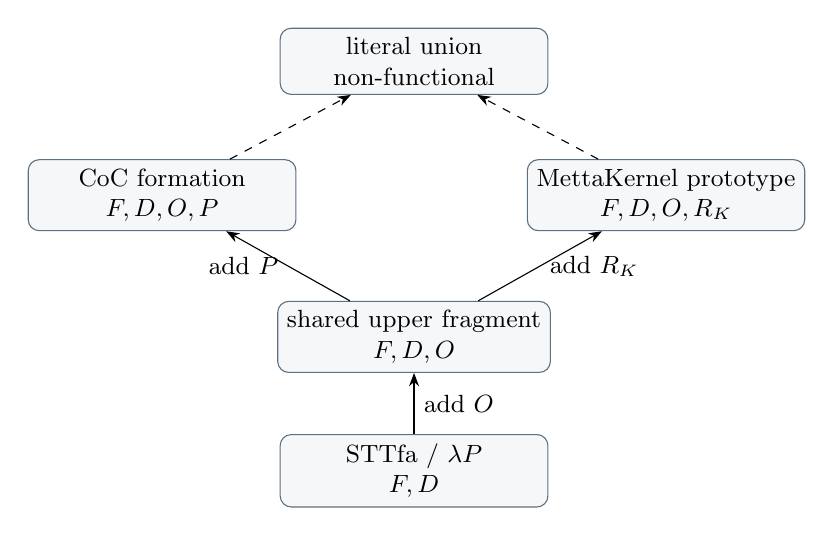
\begin{tikzpicture}[>=Stealth, every node/.style={align=center,font=\small},
  profile/.style={draw=ink!70,rounded corners,fill=ink!4,minimum width=34mm}]
\node[profile] (hub) at (0,0) {STTfa / $\lambda P$\\$F,D$};
\node[profile] (shared) at (0,1.7) {shared upper fragment\\$F,D,O$};
\node[profile] (coc) at (-3.2,3.5) {CoC formation\\$F,D,O,P$};
\node[profile] (prototype) at (3.2,3.5) {MettaKernel prototype\\$F,D,O,R_K$};
\node[profile] (union) at (0,5.2) {literal union\\non-functional};
\draw[->] (hub) -- node[right] {add $O$} (shared);
\draw[->] (shared) -- node[left] {add $P$} (coc);
\draw[->] (shared) -- node[right] {add $R_K$} (prototype);
\draw[dashed,->] (coc) -- (union);
\draw[dashed,->] (prototype) -- (union);
\end{tikzpicture}
\end{center}

The dashed union is a warning, not an admitted profile. It contains two rules
with the same domain and codomain sorts but different result sorts, and is
therefore not functional. The maintained uniqueness-of-types theorem uses
functionality. Non-functionality alone is not inconsistency, but it means that
blindly collecting both petals loses that metatheoretic route. A useful common
extension must resolve or stratify the result-sort choice, or prove another
adequate checking theory.
\lean{HypercubeHOLHub.constructionMettaKernelPrototypeUnion_not_functional, HypercubeHOLHub.mettaKernelPrototype_does_not_support_directFormationInterfaces, HypercubeHOLHub.constructions_do_not_contain_DTTBench}

A coarser semantic readout can nevertheless forget the syntactic conflict.
For this literal union, observed result sorts are functional exactly when the
readout identifies \(\mathsf{Type}\) and \(\mathsf{Kind}\). A constant
one-point readout does so; every injective readout refuses. This supplies a
common semantic shadow, not a common faithful calculus or a model of typing
and conversion. Adding \(\mathsf{Type}:\mathsf{Type}\) is a different
syntactic construction, and the maintained PTS development proves that
profile inconsistent.
\lean{HypercubeProfileStratification.constructionMettaKernelPrototypeUnion_resultFunctionalUnder_iff, HypercubeProfileStratification.constant_observation_reconciles, HypercubeProfileStratification.injective_observation_does_not_reconcile, TypeInTypeParadox.typeInType_inconsistent}

This is an obstruction to every untagged functional upper profile over the
same two sorts, not merely to the displayed list union: any upper profile
containing both branches inherits the conflicting rules. The checked common
service therefore retains a branch mode. Each fibre is functional and has
the exact profile checker. Evidence from the shared $F,D,O$ fragment rechecks
in both fibres. The selected direct interfaces separate one direction; the
prototype-computed DTTBench demand record separates the other, although the
raw statements themselves type in both upper profiles. This mode-stratified
service is a common dispatch interface, not a merged calculus. Removing the
tag requires resolving the result sort, extending the sort syntax or proving
a replacement for the present uniqueness metatheory.
\lean{HypercubeProfileStratification.no_functional_common_upper, HypercubeProfileStratification.branchProfile_functional, HypercubeProfileStratification.exists_checkProof_iff_deriv, HypercubeProfileStratification.shared_evidence_rechecks_both, HypercubeProfileStratification.construction_interface_separates_branches, HypercubeProfileStratification.prototype_computedDemand_separates_profiles}

The arbitrary-sort PTS generalization sharpens ``extending the sort syntax.''
A sort-renaming morphism preserves axioms and product rules and transports
annotated terms, beta conversion, contexts and complete typing derivations.
The existing two-sort calculus is equivalent to its generic instance. Suppose
the CoC and prototype maps into one functional target agree on their shared
$\ast$ and $\square$. Their conflicting $(\square,\ast)$ rules force the two
target images to coincide. The image of $\ast:\square$ is then $u:u$, and the
image of $(\ast,\ast,\ast)$ supplies the product rule used by the maintained
Hurkens term. Transporting that concrete derivation inhabits
$\Pi p:u.\,p$ in the target. This proves an inconsistency witness for every
functional commuting cocone, rather than merely observing a non-functional
two-sort union.
\lean{GenericPureTypeSystem.Derives.map, GenericPureTypeSystem.TwoSort.derives_iff, HypercubeSortRenaming.commuting_functional_cocone_collapses, HypercubeSortRenaming.commuting_cocone_self_axiom, HypercubeSortRenaming.commuting_cocone_self_product, HypercubeSortRenaming.commuting_functional_cocone_inconsistent}

There is also a functional three-stratum comparison target. It sends CoC's
$\ast,\square$ to $\mathsf{Prop},\mathsf{Type}_0$ and sends the prototype's
$\ast,\square$ to $\mathsf{Type}_0,\mathsf{Type}_1$. The seven image rules
are single-valued, the displayed CoC polymorphic identity and a prototype
type operator transport, and none of the three strata types itself. The maps
disagree on both source sorts. Consequently this is a noncommuting span for
comparison and reuse, not a join of the shared source calculus. It is not
named ECC or CIC: cumulativity, a model, normalization and decidable checking
remain independent obligations. The branch-tagged service above therefore
remains the faithful common interface for the original syntax.
\lean{HypercubeSortRenaming.comparisonProfile_functional, HypercubeSortRenaming.comparisonProfile_no_self_axiom, HypercubeSortRenaming.comparison_maps_disagree_on_type, HypercubeSortRenaming.comparison_maps_disagree_on_kind, HypercubeSortRenaming.coc_polymorphicIdentity_transports, HypercubeSortRenaming.prototype_typeOperator_transports}

The formation part of this policy is executable. A finite checker compares
every pair of product rules with the same premise sorts and accepts exactly
when their result sorts agree. Joining erases duplicate rules and refuses an
otherwise non-functional union. Dependency plus type operators passes; CoC
plus the MettaKernel prototype refuses. Every admitted join contains both input
profiles, and acceptance of a finite proof tree in either input yields finite
accepted evidence in the joined profile through the existing exact
profile-parametric checker.
\lean{HypercubeHOLHub.functionalProductsCheck_eq_true_iff, HypercubeHOLHub.functionalProducts_iff_profileFunctional, HypercubeHOLHub.admitProductJoin_eq_some_iff, HypercubeHOLHub.admitProductJoin_eq_none_iff, HypercubeHOLHub.dependent_operator_join_accepted, HypercubeHOLHub.coc_mettaKernelPrototype_join_refused, HypercubeHOLHub.admitted_join_rechecks_left, HypercubeHOLHub.admitted_join_rechecks_right}

The corresponding MeTTa-data boundary is also checked. A tagged atom wire
records both sort axioms and every ordered product rule. Decoding is a left
inverse of encoding, hence the representation is injective. The atom-level
join service decodes both submissions, requires identical sort axioms, then
runs the formation gate. Every published result contains both input profiles
and is functional. Dependency plus type operators is accepted; a conflicting
sort axiom, the nonfunctional CoC/prototype union and malformed atom data are
all refused. This is a source contract for a runtime consumer; it does not
claim that a current executable consumes the wire or preserves its cost.
\lean{LFProfileAtomWire.decode_encode, LFProfileAtomWire.encode_injective, LFProfileAtomWire.sameSortAxiomsCheck_eq_true_iff, LFProfileAtomWire.admitProfileJoin_sound, LFProfileAtomWire.joinEncoded_sound, LFProfileAtomWire.dependent_operator_join_encoded, LFProfileAtomWire.coc_mettaKernelPrototype_join_encoded_refused, LFProfileAtomWire.conflicting_sort_axiom_join_refused, LFProfileAtomWire.malformed_profile_refused}

This is an admission rule for formation profiles, not conversion packages.
The join of two bubbles is their least upper bound as a conversion relation,
and typing from each side embeds in it. Decidability and normalization of that
join require the separate completion, commutation or disjointness laws already
stated by the bubble theory. A runtime profile service should therefore keep
formation admission and conversion-package admission as two checks.
\lean{BubbleConversion.convertible_join_least, BubbleConversion.hasTypeIn_join_left, BubbleConversion.hasTypeIn_join_right, BubbleConversion.join_normalizedBy}

The conversion side has a parallel finite wire for the existing typed HOL
recipe policy. A manifest selects beta and eta globally or at named simple
types, and selects all or individual licensed equations. Its recursive type
codec is parameterized by a lossless codec for base-type names. Decoding is a
left inverse; malformed policies and out-of-range equation indices refuse.
Finite manifest union denotes exactly the existing pointwise policy join, so
both input local-step judgments embed in it. This gives atom-level permission
data for the HOL recipe checker. It does not yet encode a dependent-calculus
conversion package or establish normalization, confluence, decidability,
conservativity or cost for the joined policy.
\lean{HOLConversionPolicyAtomWire.enabled_join, HOLConversionPolicyAtomWire.denote_join, HOLConversionPolicyAtomWire.denote_extends_join_left, HOLConversionPolicyAtomWire.denote_extends_join_right, HOLConversionPolicyAtomWire.decodeType_encodeType, HOLConversionPolicyAtomWire.decodeFeature_encodeFeature, HOLConversionPolicyAtomWire.decode_encode, HOLConversionPolicyAtomWire.encode_injective, HOLConversionPolicyAtomWire.joinEncoded_sound, HOLConversionPolicyAtomWire.beta_eta_manifest_join, HOLConversionPolicyAtomWire.out_of_range_equation_refused, HOLConversionPolicyAtomWire.malformed_policy_refused}

\paragraph{The reified-index branch has its own exact price.}
The alternative to direct indexing can be specified rather than merely named.
A beta-correct quote/splice interface gives a split readout from retained code
to its body. A code-indexed family descends to that body view exactly when its
fibre at every code is equivalent to its fibre at the canonical
quote-after-splice code. Ordinary source equality descends exactly when the
readout is faithful, equivalently when quote after splice satisfies eta.
Thus beta supplies a body view; eta is the additional condition for forgetting
code identity.
\lean{ContextualCodeObserverFactorization.familyFactorization_iff_quoteSpliceFibreEquivalences, ContextualCodeObserverFactorization.equalityFamilyFactorization_iff_quoteSplice}

The tagged-code control is the negative half. A body-constant family descends,
while a family depending on a retained Boolean code tag does not; source
equality does not descend either. A Tarski-style encoding has another layer:
factorization of its code carrier does not imply factorization of decoding.
The maintained example has one code at each of two identified levels, but
that code decodes to a singleton at one level and Booleans at the other.
Code syntax factors and decoding cannot. Consequently a reified route owes
value/code coherence and code/meaning coherence separately. This route can
avoid the direct syntactic premise only by changing the interface; it does
not derive the missing formation rule.
\lean{ContextualCodeObserverFactorization.Canary.contextual_code_observer_boundary, TarskiCodeFamilyObserverFactorization.Canary.code_syntax_does_not_determine_decoding_factorization, TarskiCodeFamilyObserverFactorization.Canary.constant_decoding_pi_sigma_control}

The formation branch is now concrete in the same annotated PTS as the direct
necessity theorem. Direct indexing forms (P\,x) from ordinary functions and
the value-to-type rule. Type reification instead forms

\[
  Q : \mathrm{Type}\to\mathrm{Type}
  \;\vdash\;
  \Pi X:\mathrm{Type}.\,\Pi x:X.\,Q\,X
\]

from ordinary functions, polymorphism and type operators. These rule sets are
incomparable: each supports its displayed interface and refuses the other,
independently of conversion. Both universal types are accepted by the sound
reference checker at structural fuel five. The direct application is accepted
at fuel five; the reified application first consumes a type code and then its
witness, and is accepted first at fuel six. In the concrete controls its term
has five syntax nodes rather than three. The direct result type contains the
runtime argument; the reified result contains the type code and omits the
witness. Thus witness substitution is replaced by code transport plus the
separate value/code and decoding-coherence obligations above. These are exact
measurements of this syntax and checker, not asymptotic complexity claims.
\lean{ReifiedIndexElaboration.productRule_mem_of_typed_subject, ReifiedIndexElaboration.reifiedTypeIndexedForall_iff, ReifiedIndexElaboration.direct_reified_formation_fork, ReifiedIndexElaboration.directApplicationContext_formed, ReifiedIndexElaboration.reifiedApplicationContext_formed, ReifiedIndexElaboration.Controls.directApplication_accepts_fuel_five, ReifiedIndexElaboration.Controls.reifiedApplication_refuses_fuel_five, ReifiedIndexElaboration.Controls.reifiedApplication_accepts_fuel_six, ReifiedIndexElaboration.Controls.application_node_counts, ReifiedIndexElaboration.Controls.result_transport_surface, ReifiedIndexElaboration.Controls.formation_with_missing_decoding_coherence}

Here ``quotation'' and ``splicing'' name the abstract contextual-code
operations of the modal theorem. They do not redefine the candidate runtime's
surface forms. Its \code{quote} remains an evaluation-blocking constructor whose
interior variables remain available to structural matching. The distinct
\code{@} form retains its name-making role; matching below those names crosses
the existing \code{lift} boundary. Relating either runtime form to the modal
interface needs an adapter proving the relevant binding, beta and eta laws.

\subsection{Finite dependent evidence through the common interfaces}

The selected profile is the existing cumulative tower over natural-number
level expressions. Its syntax has dependent functions and pairs, identity
formation and reflexivity, explicit universe heads, and cumulativity. Its
formation-sensitive typing relation has fourteen rules. Constants and root
computations are parameterized in the general construction; this particular
tower declares neither. Structural beta computation remains available.
Only this declared mathematical profile is instantiated here.

Local codes contain syntax and rule selections. In the conversion rule they
contain an existing finite structural conversion code. Decoding checks the
local universe, declaration and head conditions and checks that conversion
code; it does not receive a proof of conversion as executable input. The
decoded node is an instance of the independently defined rule signature.
The common tree and DAG replay algorithms therefore preserve the original
premise positions and dependent substitutions. The maintained structural
replay checker also publishes common checked judgments directly, and its
existing telescope certificates check the ambient context.

\begin{theorem}[Exact finite authority for the selected judgment]
For the selected tower, a formation-sensitive judgment in a formed telescope
holds if and only if there is an accepted finite request. Such a request
checks its context, every graph row, the root address and its actual
conclusion. Raw typing derivability is equivalently accepted tree evidence,
accepted graph evidence, or a minted common checked judgment.
\end{theorem}

\lean{FormationSensitiveChecking.typing_iff_checked_tree, FormationSensitiveChecking.typing_iff_checked_graph, FormationSensitiveChecking.typing_iff_minted, FormationSensitiveChecking.mintReplay_iff, FormationSensitiveChecking.judgment_iff_checked, Tower.Checking.coverage}

Exactness is existence of accepted evidence, not a terminating procedure
for finding it. This is a connection of scoped Lean data and checked
algorithms, not a portable serialization theorem or a refinement of CeTTa's
C implementation. The source formation-sensitive conversion is structural
conversion; the comparison into the stronger typed equality does not make
every typed eta identification a source conversion.

A raw variable rule can hold in an unformed telescope. Such a raw certificate
must not authorize a formed request. The controls also reject changed root
claims, missing roots, forward or cyclic dependencies, invalid universe
lifts, and invalid unused suffixes. Shared references retain all premise
occurrences; they do not duplicate consumable execution authority.

\subsection{The comparison to sets}

The diagram keeps the source judgment between evidence and meaning:
\begin{center}
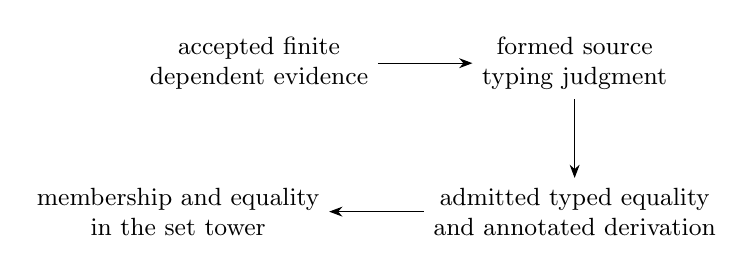
\begin{tikzpicture}[node distance=10mm and 12mm,>=Stealth,
 every node/.style={align=center,font=\small}]
\node (checked) {accepted finite\\dependent evidence};
\node[right=of checked] (source) {formed source\\typing judgment};
\node[below=of source] (typed) {admitted typed equality\\and annotated derivation};
\node[left=of typed] (model) {membership and equality\\in the set tower};
\draw[->] (checked) -- (source);
\draw[->] (source) -- (typed);
\draw[->] (typed) -- (model);
\end{tikzpicture}
\end{center}

\begin{theorem}[Checked evidence has its declared set meaning]
Under the explicit hypothesis \name{CofinalInaccessibles}, every accepted
request yields an annotated derivation whose telescope, subject and displayed
type erase to that request and whose statement holds in the existing set
tower. Checked subject values belong to their displayed type values. Finite
checked conversion between independently admitted endpoints preserves their
actual model values.
\end{theorem}

\lean{TowerInterpretation.Checking.request_model_sound, TowerInterpretation.Checking.checked_value_member, TowerInterpretation.Checking.checked_type_conversion, TowerInterpretation.Checking.checked_term_conversion}

For closed universe-membership queries the comparison also reflects the
model: a finite request for $U_c : U_d$ exists exactly when the corresponding
set universe is a member of the other. The same equivalence holds after
the existing well-founded embedding into material hypersets. This is a
scoped reflection result for universes, not completeness for arbitrary set
truth. Under the named model hypothesis, every request for a closed
inhabitant of the existing empty type is rejected.
\lean{TowerInterpretation.Checking.universe_request_iff_set, TowerInterpretation.Checking.universe_request_iff_hyperset, TowerInterpretation.Checking.empty_request_refuses}

Substitution uses the actual checked component terms. Their accepted
requests construct the source contextual arrow. At the semantic comparison
boundary, the annotated components carry their typing and erasure witnesses;
evaluation of those components constructs the satisfying-environment map.
The value of a substituted checked term equals its original value in that
substituted environment. Context and component compatibility are retained
in the statement, rather than being replaced by an assumed semantic action.
\lean{FormationSensitiveChecking.checked_substitute, TowerInterpretation.Checking.checkedArrow, TowerInterpretation.Checking.checked_value_substitution}

The model map has several distinct scopes. The cumulative tower has the
set interpretation just used, with its named inaccessible-cardinal
hypothesis. The HOTG-style mathematical packages add declared set operations
and theory assumptions; they are not automatically translations to the
native Megalodon Mathdata checker. The material hyperset family construction takes an explicit presentation
and supplies contexts, dependent families, substitution and Pi/Sigma structure.
Its extensional identity does not establish a faithful interpretation of
arbitrary higher paths, cubical operations or every dependent profile.

A useful negative boundary is the existing HOTG-style
\name{setTheory_not_admitted}: a package can have a set model while failing
its stated computational admission discipline. The rule-constant alternative
has separate preservation results. Semantic equality therefore cannot be
promoted to checker conversion merely because both expressions denote the
same set. Conversely, a model interpretation need not reflect all set truth
back into source derivations. These comparisons preserve their assumptions;
they assert neither equivalence of all foundations nor optimal native speed.

\paragraph{Native guarded transport.}
Two typed HOL schemas now transport universal and existential observations
between guarded representations. Their explicit forward and backward maps
preserve validity and are inverse on valid values. The observed predicate is
pulled back along the chosen forward map; comparison action is retained.
Both formulas hold in every Henkin model, with no full-domain or choice
premise, and their Lean proofs use no host axioms. An inhabited representation
of an empty carrier refutes the actual intrinsic formula obtained by dropping
the target guard. A Boolean swap supplies a valid nonidentity comparison,
whose action changes a selected observation.
\lean{HOL.GuardedQuantifierTransport.models_universal, HOL.GuardedQuantifierTransport.models_existential, HOL.GuardedQuantifierTransport.guard_erasure_counterexample, HOL.GuardedQuantifierTransport.Examples.swap_comparison, HOL.GuardedQuantifierTransport.Examples.swap_changes_observation}

Independent original HOL Light proofs establish the same exact statements.
The explicit-rule producer uses generalization, specialization, discharge,
conjunction, equality and existential introduction/elimination. Its exported
closure retains five checked logical definitions and has no AXIOM nodes;
the earlier proof-search route used eta and choice. Native replay under the
existing sealed policy, which prohibits axiom introduction, checks the
two exact sequents and rejects changed claims, additional axioms and a
truncated stream. Packet checks also refuse a missing or repeated root and
the typed guard-erasure claim. The maps' comparison certificates remain
requirements of clients. This library is an interoperability and
representation edge, not automatic datatype proof generation or a proof of
the linked native checker.

On the same pinned checker and standard policy, eight interleaved paired
fresh-process runs checked the identical two sequents. The proof-search
artifact used 36,205 records and 202,056 bytes; the explicit-rule artifact used
3,023 records and 16,382 bytes. Median process time was 6.51\,ms versus
2.15\,ms, and median peak RSS was 9,724 versus 8,216\,KiB. These are measured
costs of these two proof artifacts, not an optimality theorem or a bound for
other workloads. The explicit proof also qualifies under the separate sealed
policy.

The exact semantic boundary for truth observations is weaker than an inverse
comparison. Over the observation class containing every predicate, preserving
all existential truths is equivalent to the image of valid source values
being exactly the valid target values. The same equivalence holds for all
universal truths. A projection from a pair of Booleans to its first component
satisfies both observation laws while identifying distinct source values.
Truth agreement therefore does not establish faithful transport of values,
witnesses or multiplicities. The native library retains its explicit
inverse-comparison hypothesis; this semantic criterion does not change its
admission contract.
\lean{HOL.GuardedQuantifierTransport.exists_observations_iff_image, HOL.GuardedQuantifierTransport.all_observations_iff_image, HOL.GuardedQuantifierTransport.truth_transport_does_not_force_injectivity}

\subsection{Operational logical form and relative checking bases}

The choice of a low-tier checker can follow from a richer dependent theory
and the fragment requested of it. There are at least three constructions:
restrict declarations and computation rules; elaborate implicit conversion
into explicit evidence; or specialize a checking algorithm for a declared
fragment. These give different proof formats and cost profiles. A literal
syntax intersection does not decide which construction is best.

Dependent carve-outs additionally retain formed contexts, binding,
substitution, universe policies and the selected identity rules. Their
operational predicate comparison does not discharge these dependent laws or
admit an inductive schema. A fibration organizes the obligations; an
executable extraction and an optimality theorem require further evidence.

For the existing dependent calculus, every accepted formed request has a
finite sufficient restriction of its declaration and root-computation package.
The same context, subject and displayed type are derivable there, and every
judgment of that restriction reflects to the original package. This is a
constructed restriction, not a theorem that a smallest checker exists. The
universe policy is retained. Computational admission and an executable root
decoder for the restriction are additional obligations: pruning may remove
formation or preservation support required by a chosen admission discipline.
\lean{FormationSensitiveCheckingOSLF.checked_request_has_restriction, FormationSensitive.Dependencies.exists_restriction_with_reflection, FormationSensitive.RestrictionPreservation.oslf_observation_does_not_admit_restriction, FormationSensitive.RestrictionPreservation.oslf_observation_with_preserving_repair}

OSLF applies to the declared dynamics. In the conversion-evidence observation,
vertices are the original scoped terms and edges are original structural
steps with either orientation. The observation theory retains syntax equality
as its equation policy, so conversion remains visible as finite paths. Its
generated reachability native type holds exactly when the independently
authored conversion holds, equivalently when some supplied finite code checks.
Reverse beta is therefore a valid conversion edge; this does not declare it
an evaluator reduction. A raw beta path also does not establish formed typing.
\lean{FormationSensitiveCheckingOSLF.path_iff_conversion, FormationSensitiveCheckingOSLF.satisfies_iff_checked, Tower.Checking.Controls.reverse_beta_oslf, Tower.Checking.Controls.raw_beta_oslf}

Native type theory obtains richer structure through the internal languages
of presheaf toposes~\cite{WilliamsStay}. The comparison here concerns the
declared relational OSLF predicate frame and its operational routes. It does
not establish that entire presheaf construction for every dependent profile.

In the general OSLF construction, semantic predicates are invariant under the
selected equations. Closure under computation is a further property. The
existing route interfaces yield the following separate results:
\begin{center}\small
\begin{tabularx}{\linewidth}{@{}lX@{}}
\toprule
Route contract & Earned observation law \\
\midrule
Equation-respecting map & Reindex invariant predicates. Pointwise agreement
modulo target equations gives equal predicate actions. \\
Strict forward operational translation & Preserve existential one-step
observations; additional target behavior may remain. \\
Locally covered translation & Also reflect those observations and finite
reachability from image states. \\
Path-valued operational realization & Preserve finite reachability while
permitting a source step to become zero or several target steps. \\
\bottomrule
\end{tabularx}\end{center}
\lean{EquationRespectingMap.pullback_eq_of_equiv, OperationalTranslation.preserves_semanticDiamond, CoveredTranslation.semanticDiamond_iff, CoveredTranslation.semanticReach_iff, OperationalRealization.preserves_semanticReach}

The extra-target-step control refutes unrestricted reflection. The fusion
control preserves a path observation while destroying a one-step diamond.
OSLF's right-adjoint box in this construction observes incoming steps; its
transport cannot be inferred from outgoing coverage alone. Bounded-cost
observations additionally require a declared charge and a bound on mapped
paths. Predicate transport does not by itself establish those bounds, proof
translation, native seal enforcement, or equality of retained proof histories.
The basic behavioral GSLT morphism only promises bisimilarity preservation.
\lean{IndexedOperational.Canary.escaping_native_type_not_reflected, IndexedOperational.Canary.outgoing_coverage_does_not_preserve_past_box, OperationalRealization.FusionCanary.fusion_changes_one_step_diamond}

HOL Light, MM0 and Megalodon consequently remain comparison points and native
realizations with explicit source contracts. They do not exhaust the possible
checking bases for dependent profiles. A semantic set model is another
comparison edge, with its assumptions retained; it is not an executable proof
translation or a reflection theorem for arbitrary set truth. Relative
optimality needs the fragment, certificate representation, operations and
cost model to be fixed before it can be asserted.

For the selected cumulative profile, the guarded set-model comparison also
receives this OSLF conversion observation directly. Two accepted term-typing
requests in a formed telescope give equal actual set values when the
conversion-native observation holds. The annotated context and the named
model hypothesis remain explicit.
\lean{TowerInterpretation.Checking.oslf_term_conversion}

\subsection{A computational STT carve-out, with a proved boundary}

The existing one-base simply typed lambda calculus supplies a first exact
comparison. Write $S(\Gamma,A)$ for its intrinsically typed terms, $E$ for
its embedding in the root-free cumulative Pi/Sigma/identity tower, and
$H_b$ for its HOL interpretation at a chosen base sort $b$. Simple arrows
become nondependent products in $E$ and ordinary arrows in $H_b$. The chosen
base sort remains distinct from HOL's proposition sort. For every context
and simple type:
\[
 \begin{aligned}
  \operatorname{Join}_{\beta}(H_b(s),H_b(t))
   &\iff s\equiv_{\beta}t\\
   &\iff\operatorname{Conv}_{\mathrm{struct}}(E(s),E(t))\\
   &\iff\operatorname{decideConversion}(s,t)=\mathsf{true}.
 \end{aligned}
\]
The tower conversion path may leave the simple image. Reflection follows
from normalization and confluence, not an assumption that all intermediate
terms remain simple. HOL uses its independently defined operational beta
steps. Normal intrinsic terms remain normal there, so common reducts
determine the same intrinsic normal form.
\lean{SingleBaseSTLC.HOLComparison.holJoinable_iff_betaConv, SingleBaseSTLC.HOLComparison.holJoinable_iff_towerConv, SingleBaseSTLC.HOLComparison.decideConversion_iff_holJoinable}

The scope is one base sort, variables, abstractions and applications, with
no declared constants. This compares a computational judgment, not all HOL
theoremhood or arbitrary dependent inhabitants. It is a reference component
for a possible native kernel, not a completed HOL bubble or a selection among
the dependent language candidates.

The maps commute with simultaneous substitution and give a functor between
the existing context categories. An indexed family alone is not a fibration:
chosen cartesian lifts and their laws require additional constructions.
Typed HOL syntax retains intermediate application types that the unannotated
tower erasure can lose, even at a fixed result type. Conversion classes remain
faithfully compared. Raw syntax recovery and conversion reflection are
therefore different requirements on a shared representation.
\lean{SingleBaseSTLC.HOLComparison.contextFunctor, SingleBaseSTLC.HOLComparison.substitute_term, SingleBaseSTLC.HOLComparison.Controls.hol_retains_erased_types, SingleBaseSTLC.ConversionDecision.betaClass_toTower_injective}

\paragraph{Two local policies.}
The common bubble interface now has a simple-term instance. Beta steps retain
HOL operational evidence; a second policy additionally permits eta, with
application and abstraction congruence in both policies. Free conversion trees
retain their composition and intermediate states. Each tree elaborates
constructively to an ordinary retained HOL equality proof with the same
endpoints. The beta-only policy presents exactly the structural tower
conversion above.
\lean{SingleBaseSTLC.HOLConversionBubble.elaborate, SingleBaseSTLC.HOLConversionBubble.beta_path_iff_tower}

For an arrow-typed variable $f$, the terms $f$ and $\lambda x.fx$ are
beta-normal and not beta-convertible, although the eta policy relates them
and HOL proves their equality. The tower's \emph{typed-equality} judgment also
contains eta; its \emph{structural conversion} in the comparison does not.
Even two judgments over one package cannot be interchanged silently.
An equality theorem does not automatically license definitional computation.
Arbitrary additional rewrite packages would need fresh admission obligations.
\lean{SingleBaseSTLC.HOLConversionBubble.Controls.eta_strictly_adds_conversion, SingleBaseSTLC.HOLComparison.Controls.hol_equality_does_not_reflect_conversion, SingleBaseSTLC.HOLTowerModel.typed_equality_not_structural_conversion}

\paragraph{Operational predicates, dependent readings and models.}
This conversion observation and the earlier dependent checking development
reuse one general construction for the equivalence closure of an authored
relation. Equations of the observation theory are syntax equality;
bidirectional computation edges remain visible. Its OSLF reachability
predicate has exactly the support of retained conversion trees. On the beta
fragment the existing total intrinsic normal-form comparison decides it.
Predicate truth does not reconstruct a particular history.
\lean{IndexedOperational.conversionTheory_path_iff, IndexedOperational.satisfies_conversionNativeType_iff, SingleBaseSTLC.HOLConversionBubble.satisfies_iff_path, SingleBaseSTLC.HOLConversionBubble.beta_satisfies_iff_decides}

Every lawful dependent \name{HOLReading} reads these pure simple terms
without interpreting additional constants or supplying an equality-proof
algebra. Their computed codes are typed in that reading's actual selected
judgment. The maintained native substitution constructor has no unread image
on this fragment, and code commutes with substitution. The beta observation
thus gives typed equality of the computed codes. This is a parametric
inclusion result with explicit reading laws, not reflection from arbitrary
dependent proofs.
\lean{SingleBaseSTLC.HOLReadingComparison.code_typed, SingleBaseSTLC.HOLReadingComparison.code_substitute, SingleBaseSTLC.HOLReadingComparison.observed_typed}

For the tower, the independently formed simple context and admitted equality
reach its maintained annotated set interpretation under the named
\name{CofinalInaccessibles} hypothesis. That hypothesis belongs to the
semantic edge, not the beta decision procedure. The earlier well-founded
embedding into material hypersets retains its stated scope; neither result
supplies arbitrary higher identities or a translation to native Mathdata.
\lean{SingleBaseSTLC.HOLTowerModel.observed_set_equality}

\paragraph{From a component to a whole HOL bubble.}
Choice, infinity and classical principles belong to a declared theory and
its interpretations; conversion policy belongs to the judgment. Option names
are not independence proofs for their combinations. The existing HOL calculus,
retained derivations and theory interfaces supply these logical profiles.
Merely naming another kernel does not require copying their rules.

A complete proof-level carve-out needs a rule-preserving interpretation into
the selected dependent judgment and a genuine reflection or conservativity
argument for the declared image. Type-shape membership supplies neither.
Routes to native HOL Light, Megalodon and configured MM0 must retain their own
assumptions, definitions, equality policies and evidence. This comparison
establishes no new complete three-way translation.

A suitable tier-zero realization can specialize a richer checker, or expose
its implicit computation as explicit evidence. It need not be a literal
subset of the checker's source or add an interpreter layer to a qualified
native operation. Direct normalization, finite replay, optional proof
recording and protected theorem authority have separate contracts. Choosing
their best physical realization requires workload and cost comparisons.

\subsection{Conversion policies, proof elaboration and operational fibres}

A checking graph needs more than an ordering of mathematical strength.
One edge may add an axiom, another may license a formerly explicit equality
as conversion, and another may change only the producer of certificates.
An interpretation, a conservative extension and a measured specialization
carry different laws. Distinct proof and execution histories remain visible
until an observation explicitly forgets them.

The current HOL reference instance fixes arbitrary base sorts and typed
constants, while a policy selects beta permissions by the contracted
redex's result type, eta permissions by domain and codomain, and equation
permissions by declaration occurrence. The permission is checked at the
actual inner redex, even when the surrounding term has another type.
A cited equation carries its pattern telescope and a simultaneous
substitution. Explicit typed substitution contexts and abstraction/quantifier
congruence support computation under binders without dropping scope.
A substitution context can use its parameter repeatedly; this derived
equality action is not necessarily one evaluator contraction.

For a policy $P$, let $R_P$ be the independently stated local-step relation.
The maintained equality-recipe checker computes endpoints, checks every
transitivity join and has exact authority:
\[
 s\;\operatorname{EqvGen}(R_P)\;t
 \quad\Longleftrightarrow\quad
 \exists e.\;\operatorname{check}_P((s,t),e)=\mathsf{true}.
\]
This is a decision about a supplied finite article. It does not require a
normalizer or decide whether some article exists. The generic decoder
constructs a free conversion tree from successful replay; forgetting that
tree recovers the submitted recipe exactly, including its local witnesses
and binary composition structure.
\lean{EqualityRecipe.checkedPathWithRecovery, EqualityRecipe.forget_checkedPath, HOL.ConversionRecipes.leaf_authority, HOL.ConversionRecipes.authority}

The existing typed beta-execution carrier also compiles directly into these
recipes, retaining each contracted position. A previous beta-joinability
witness consequently supplies an accepted beta-only article. This is a
computed forward connection to the maintained operational component; it does
not assert reverse reflection for every policy or equality of proof histories.
\lean{HOL.ConversionRecipes.executionRecipe, HOL.ConversionRecipes.executionRecipe_checked, HOL.ConversionRecipes.joinable_has_betaRecipe}

\begin{center}
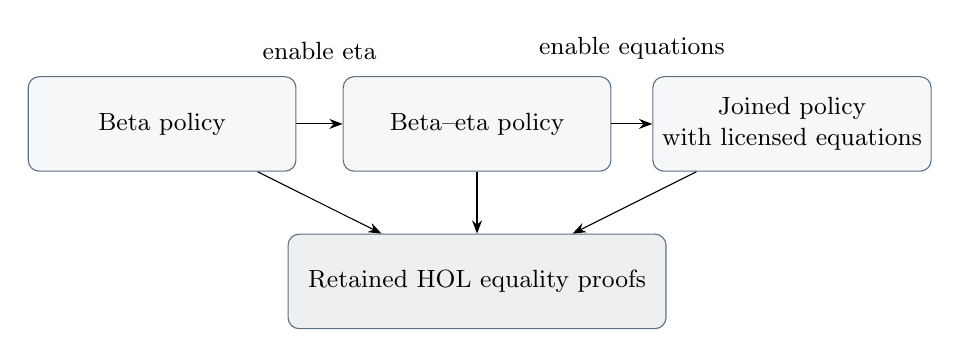
\begin{tikzpicture}[>=Stealth, font=\small,
  policy/.style={draw=ink!70, rounded corners, fill=ink!4,
    align=center, minimum width=34mm, minimum height=12mm},
  target/.style={draw=ink!70, rounded corners, fill=ink!8,
    align=center, minimum width=48mm, minimum height=12mm}]
  \node[policy] (b) at (-4,0) {Beta policy};
  \node[policy] (be) at (0,0) {Beta--eta policy};
  \node[policy] (bed) at (4,0) {Joined policy\\with licensed equations};
  \node[target] (hol) at (0,-2) {Retained HOL equality proofs};
  \draw[->] (b) -- node[above=7mm] {enable eta} (be);
  \draw[->] (be) -- node[above=7mm] {enable equations} (bed);
  \draw[->] (b) -- (hol);
  \draw[->] (be) -- (hol);
  \draw[->] (bed) -- (hol);
\end{tikzpicture}
\end{center}
The downward edges use actual retained equality receipts for each equation,
at its original telescope. They construct ordinary HOL proofs through beta,
eta, congruence and equality composition. Logical retyping becomes explicit
propositional equality elimination. The two-sort controls reach the same
endpoint equality by primitive eta and by an instantiated eta declaration,
while the submitted receipts remain distinct. Another pair has the same
endpoint equality and retained proof sizes one and three. These are proof
sizes, not elapsed-time comparisons.
\lean{HOL.EquationProofs.instantiate, HOL.ConversionRecipes.elaborate, HOL.ConversionRecipes.convertProof, HOL.ConversionRecipes.Controls.eta_and_equation_recipes_distinct, HOL.ConversionRecipes.Controls.proof_costs_differ}

The existing implication/universal modulo calculus stores
proposition-valued conversion. With the same equation receipts, every one
of its proofs has an ordinary retained HOL proof at the original ordered
sequent. This translation establishes existence; it does not reconstruct a
forgotten source history. The checked recipe interface supplies that stronger
reconstruction. Curry's cyclic equation cannot acquire the required HOL
receipts: otherwise its existing modulo proof of $\forall p.p$ would become
an ordinary HOL proof, contradicting the maintained standard model.
These edges cover equations already justified by the target calculus.
Fresh definitional extensions instead use the separate signature-changing
unfolding and conservativity construction.
\lean{HOL.ProofSyntaxModulo.hasHOLProof, HOL.ConversionElaborationControls.no_curry_equationProofs, HOL.ProofSyntaxModulo.definition_conservative}

\paragraph{What composes.}
Two rule packages independently admissible over the \emph{same original}
judgment system can be combined without changing derivability. Actual local
certificate compilers also combine, selecting each feature's own expansion
and node budget. The mixed control eliminates a shortcut and an identity
inference into a three-node base certificate; adjoining the genuinely new
fact still has no such compiler. This logical composition law does not
establish normalization, confluence or decidability for a union of
conversion engines. Those are separate interaction obligations.
\lean{extendRules_union_sameDerivability_iff, AdditionalRuleCertificateCompiler.combine, AdditionalRuleCertificateCompiler.combine_sameDerivability, ConservativeExtensionCanary.compiledMixed_count, ConservativeExtensionCanary.combined_newFact_forbidden}

\paragraph{Elaboration and execution.}
An elaborator may perform implicit-argument search, instance resolution,
unification or tactics. Here an arbitrary producer submits finite recipes
to the existing screening interface, and only accepted submissions acquire
retained equality proofs. Producer completeness is unnecessary for this
soundness boundary. This is a concrete consumer of the producer/checker
separation, not an implementation of all those frontend algorithms.
\lean{HOL.ConversionRecipes.elaborateSubmission, HeuristicEvidence.arbitrary_producer_sound}

The operational fibre over a context, type and policy has the original typed
terms as states. Its OSLF reachability predicate is exactly certificate
existence for $\operatorname{EqvGen}(R_P)$. Policy extensions and joins
preserve this observation, including computations under binders. This
predicate forgets the chosen recipe; the recipe decoder does not.
Program-execution fibres additionally retain the chosen world, resources,
representation and scheduling policy. Their routes use the earlier strict,
covered or path-valued operational contracts as appropriate. Logical
conversion is not thereby declared to be evaluator reduction, and execution
costs need their own accounts.
\lean{HOL.ConversionRecipes.observed_iff_accepted, HOL.ConversionRecipes.LocalStep.conversion_mono, HOL.ConversionRecipes.observed_mono}

\paragraph{Extensional comparisons remain selected bridges.}
Modular type-theory presentations provide an established precedent for
feature-selected fragments~\cite{ModularTheories}. Hofmann's comparison of
specified extensional and intensional theories, with functional
extensionality and UIP on the intensional side, concerns an interpretation
and conservativity, rather than identical conversion algorithms. The later
Morita-equivalence result compares their categories of models in its stated
setting~\cite{HofmannExtensional,KapulkinLi}. These results do not establish
such a bridge for every dependent candidate in this library. A semantic
extensional readout can coexist with an executable intensional checker and
explicit transport evidence, without making equality reflection a rule of
every checker. Chosen route action, universe policy, theory assumptions and
operational observations remain part of the comparison.

The new checker is a proof-producing reference on already scoped and typed
syntax. It qualifies neither a raw-byte parser nor native seal enforcement,
and it supplies no native performance comparison. Full dependent-fragment
reflection and the routes to actual HOL Light, Mathdata and configured MM0
remain further graph edges.

\subsection{Selected iota roots and checked dependent instantiation}

The existing \name{ParameterizedPiSigmaId} rules already state the head,
universe, cumulativity, constant and root-computation policies of that
calculus. Its indexed-family interface separately carries constructors,
an eliminator specification and typed iota schemas. The following checking
connection consumes those schemas; it does not derive another eliminator
or introduce a universal profile record for every dependent candidate.

An ordered schema table $T$ stores open endpoint pairs at their respective
arities. A policy $e:\operatorname{Fin}|T|\to\mathsf{Bool}$ selects original
row occurrences. A finite root code supplies a row address and a list of
scoped arguments. Replay checks the address, permission and argument count,
then computes capture-safe simultaneous substitution into the selected pair.
The independently defined root evidence retains both the original row and
the substitution. Its decoder is sound and complete for exactly those
instances. Repeated equal rows remain distinct citations, and an enabled
duplicate cannot rescue a disabled citation.
\lean{SchemaTableConversionCode.retained, SchemaTableConversionCode.decode_sound, SchemaTableConversionCode.decode_complete, SchemaTableConversionCode.rootDecoder}

Renaming and substitution act on every submitted argument while retaining
the row address. Replay commutes with these actions, including refusals.
Selection by schema occurrence is stable under substitution. A selection
depending on the instantiated dependent type would need its own stability
law before becoming a root-computation policy.
\lean{SchemaTableConversionCode.decode_rename, SchemaTableConversionCode.decode_substitute}

For a table of existing typed iota schemas, row lookup also retrieves the
original telescope $\Gamma_i$, displayed type $A_i$ and retained computation
witness. The selected rule package keeps the original head, universe and
constant policies and replaces its authored roots by the selected instances.
Unlisted inherited and delta roots are excluded from this restriction.
The signature's stated correspondence between retained witnesses and raw
declared computation gives an actual rule morphism into the original
declaration calculus. It preserves full formation-sensitive judgments and
induces a forward OSLF conversion route. No reverse coverage, normalization
or admission theorem is inferred from this inclusion.
\lean{IndexedFamily.Checking.receiptAt, IndexedFamily.Checking.realizeEvidence, IndexedFamily.Checking.inclusion, IndexedFamily.Checking.judgment_inclusion, IndexedFamily.Checking.conversionRoute}

\paragraph{Typed instantiation is another finite check.}
At a caller's telescope $\Delta$, a substitution request checks formation of
$\Delta$ and each dependent argument obligation
\[
  \Delta\vdash\sigma(v):\sigma(\Gamma_i(v)).
\]
The maintained telescope and structural typing checkers perform these checks.
Even a zero-argument request must check $\Delta$: an empty argument list
cannot authorize an unformed context. Every admitted formation-sensitive
context morphism has such finite evidence; this is certificate existence,
not an inference procedure.
\lean{FormationSensitiveChecking.SubstitutionRequest.sound, FormationSensitiveChecking.SubstitutionRequest.complete}

With a permitted row, accepted arguments and the exact requested endpoints
and displayed type, replay substitutes the original typed receipt. It
retains both endpoint typings and the original computation witness at
$\sigma(A_i)$. The same request exports a finite raw root code. The reverse
implication fails: raw computation does not establish argument typing.
Disabling a computation permission also does not construct a propositional
identity proof in the smaller calculus.
\lean{IndexedFamily.Checking.InstanceRequest.replay, IndexedFamily.Checking.InstanceRequest.formed, IndexedFamily.Checking.InstanceRequest.rootCode_accepted}

\paragraph{The existing natural/vector instance.}
The cumulative declaration signature has four independently defined iota
cases: natural zero and successor, and vector nil and cons. Its actual four
canonical schemas now give an exact decoder for that original root relation.
The declaration decoder then combines inherited computation, actual delta
lookup and these four cases. This supplies the missing executable parameter
of common conversion and formation-sensitive judgment checking for the
unchanged signature.
\lean{NativeNaturalVectorFamilies.Checking.iotaDecoder, NativeNaturalVectorFamilies.Checking.decoder, NativeNaturalVectorFamilies.Checking.conversion_iff_checked, NativeNaturalVectorFamilies.Checking.coverage}

The controls check all four raw iota cases, an actual typed natural-eliminator
instance in its dependent telescope, and its weakening to a larger context.
They reject exchanged dependent arguments, a changed displayed type,
incorrect arities, captured endpoints and disabled rows. An instance with
unknown arguments has raw computation evidence but fails the typed instance check.
The retained natural iota receipt is reconstructed by the checker, rather
than supplied as part of its untrusted request.
\lean{IndexedFamilyCheckingControls.all_verdicts, IndexedFamilyCheckingControls.checkedZeroReceipt}

These results do not qualify uniform preservation of the raw signature,
general positivity checking, or native execution of vector programs.
The earlier root-free set comparison does not
automatically interpret these added declarations. Natural infinity and no-confusion require
their own constructor and induction laws; finite datatype declarations have
different consequences. Translation of those laws to HOL Light, Mathdata or
configured MM0, and a native realization of this checker, remain separate
edges. Partial checking and operational contracts can therefore enter the
graph without pretending that every node already discharges every contract.

\subsection{Generated rules, bidirectional evidence and dependent append}

The simple-inductive generator already produces its recursor and one iota
schema per source constructor occurrence. Its computation relation is stated
independently of schema replay. The generated ordered table now presents
exactly that relation, and the common finite decoder checks the resulting
conversion recipes. A receipt retains its constructor ordinal and complete
assignment; it translates directly to a single checked root, including below
binders. This connection does not identify raw conversion evidence with the
generator's annotated typed receipts or establish declaration admission.
\lean{IndexedPolynomialGenerated.Checking.presents, IndexedPolynomialGenerated.Checking.table_get, IndexedPolynomialGenerated.Checking.receiptCode_accepted, IndexedPolynomialGenerated.Checking.conversion_iff_checked}

The bidirectional producer works against a selected existing rule package.
It synthesizes types for variables, declared constants and applications,
and checks lambdas and pairs against dependent products and sums. Its inputs
include proposed head types, universe joins, normalizations and conversion
recipes. These proposals carry no logical authority: every successful
submission passes the maintained context and formation-sensitive judgment
checkers. Soundness therefore holds even for incorrect producer choices.
Fuel bounds the search; refusal is not a proof of nontypability.
\lean{FormationSensitiveElaboration.replay_sound, FormationSensitiveElaboration.elaborate_sound}

Restricted implicit inference reuses the existing scoped schema matcher.
Argument-type patterns share one assignment, so repeated metavariables must
agree. Every omitted prefix argument must be determined; no arbitrary value
fills an unconstrained slot. The resulting application, with implicit
arguments followed by the original explicit arguments, undergoes the same
independent checking. For vector cons, the explicit head and tail determine
both element type and length. Controls reject an undetermined length,
inconsistent repeated element types and missing or extra arguments. This is
not a complete higher-order unifier or an instance-resolution algorithm.
\lean{FormationSensitiveElaboration.Implicit.complete_sound, FormationSensitiveElaboration.Implicit.elaborate_sound, InductiveElaborationControls.inferredSingleton_typed}

Conversion search traverses the maintained syntax and proposes explicit
beta, projection, congruence and declaration-root recipes. Each proposed
normalization is checked against its original endpoints. Comparing two such
results constructs a recipe through their common shape and checks the
composite again. The soundness theorems establish conversion, not normal-form
existence, completeness of search or forward evaluation of every returned
conversion recipe.
\lean{StructuralConversionSearch.normalize_sound, StructuralConversionSearch.compare_sound}

\paragraph{A checked dependent function.}
The independently authored cumulative Nat/Vec declaration has an element
universe parameter $u$ and a motive parameter $v$. The existing
level-instantiation morphism specializes the latter to $\max(u,v)$, retaining
both parameters and transporting declaration formation. This licenses the
vector-valued motive needed by the following explicit core program:
\[
  \mathsf{append} : \Pi(A:U_u).\Pi(n,m:\mathsf{Nat}).
    \mathsf{Vec}\ A\ n \to \mathsf{Vec}\ A\ m
    \to \mathsf{Vec}\ A\ (\mathsf{add}\ n\ m).
\]
Addition uses the declared natural eliminator, and append uses the declared
vector eliminator. Neither introduces new recursion or conversion rules.
The proof checks the entire closed function at this dependent type in the
selected instance, with its schematic element universe and both lengths.
\lean{NativeNaturalVectorFamilies.Programs.levelInstance, NativeNaturalVectorFamilies.Programs.signature_formed, NativeNaturalVectorFamilies.Programs.judgment_map, NativeNaturalVectorFamilies.Programs.append_typed}

Evidence production runs outside the proof kernel. A shared constructor-data
emitter records its finite submission; kernel reduction then checks only
that data against the independently written program, type and decoder.
The qualified append submission uses 962 shared definitions in 387836 bytes
of Lean source. The checker rejects the same submission with its result
index changed, its program replaced by the second input vector, or its root
typing rule forged. These refusals concern the submitted evidence, rather
than general unprovability of other claims.
\lean{NativeNaturalVectorFamilies.Programs.appendChecked_true, NativeNaturalVectorFamilies.Programs.changedType_refused, NativeNaturalVectorFamilies.Programs.changedTerm_refused, NativeNaturalVectorFamilies.Programs.forgedRoot_refused}

The nil and cons equations of this program hold under arbitrary scoped
substitutions. In the cons equation the target contains append applied to
the recursive tail; retaining the unprocessed tail instead is refused by
the comparison check. These results establish structural conversion, rather
than a forward execution strategy or a termination theorem.
\lean{NativeNaturalVectorFamilies.Programs.Computation.append_substitute, NativeNaturalVectorFamilies.Programs.Computation.append_nil, NativeNaturalVectorFamilies.Programs.Computation.append_cons}

\paragraph{Constructor clauses and checking permissions.}
A scoped clause compiler consumes the admitted constructor inventory.
Its current fragment has one linear, top-level clause per constructor, in
source order. The compiler checks names and field counts, replaces written
calls on the declared recursive children by induction hypotheses, and
constructs methods for the existing eliminator. Capture-safe inverse
substitution certifies that replacing those hypotheses by their original
calls reconstructs the submitted clause. Whole-term elaboration still uses
the independent formation-sensitive checker.
\lean{ScopedSubstitutionInversion.invert_sound, IndexedInductive.CaseElaboration.compileBranch_reconstructs, IndexedInductive.CaseElaboration.compileMethods_coverage, IndexedInductive.CaseElaboration.elaborate_sound}

For the admitted vector inventory, the written append clauses compile to
exactly the independently authored core function above, uniformly in the
payload type. Controls refuse missing, extra or reordered clauses, incorrect
field counts, calls on another child or index, and a remaining recursive
function constant. The concrete source interface includes a noncomputable
interpretation of natural indices: this is a kernel-evaluated comparison,
not an executable textual frontend. Nested pattern matrices and their
compilation remain outside this clause fragment.
\lean{IndexedInductive.AppendElaboration.methods_match_reference, IndexedInductive.AppendElaboration.compiled_matches_reference, IndexedInductive.AppendElaboration.compiled_typed, IndexedInductive.AppendElaboration.all_verdicts}

The same finite append typing submission also checks in an actual restricted
calculus containing just the two natural iota rows, with unchanged heads,
declarations and universe instance. Removing either row rejects that
submission. The vector rows remain separate permissions for computing
vector eliminator applications. Monotone permission inclusions preserve
full judgments and their original contexts. Thus a smaller checking basis
can be derived from a richer declared judgment, without claiming a globally
smallest kernel or unprovability from the rejected submissions. These local
results do not establish uniform computational admission of the package.
\lean{NativeNaturalVectorFamilies.Programs.ComputationProfiles.permissions_mono, NativeNaturalVectorFamilies.Programs.ComputationProfiles.judgment_inclusion, NativeNaturalVectorFamilies.Programs.ComputationProfiles.append_typed_naturalOnly, NativeNaturalVectorFamilies.Programs.ComputationProfiles.all_verdicts}

\paragraph{Finite manifests for the checking-profile flower.}
The same admitted schema table has four explicitly separated checking nodes.
The minimal node retains every typed iota receipt but licenses no iota
conversion. The natural intensional node adds exactly the two natural rows.
It has two incomparable children: the scoped logical-extensional node adds
opaque propositional and function extensionality as object-theory constants,
while the raw operational node licenses both vector rows. Neither child
silently supplies the other's capability.
\begin{center}
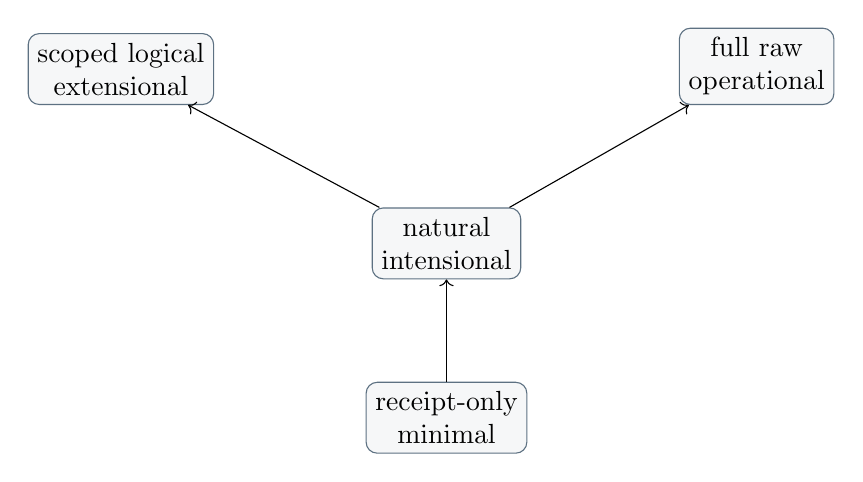
\begin{tikzpicture}[
  node distance=13mm and 20mm,
  every node/.style={draw=ink!70,rounded corners,fill=ink!4,align=center}]
\node (minimal) {receipt-only\\minimal};
\node (natural) [above=of minimal] {natural\\intensional};
\node (logical) [above left=of natural] {scoped logical\\extensional};
\node (raw) [above right=of natural] {full raw\\operational};
\draw[->] (minimal) -- (natural);
\draw[->] (natural) -- (logical);
\draw[->] (natural) -- (raw);
\end{tikzpicture}
\end{center}
Inclusion and both reverse separations are checked per capability field. The
logical child keeps extensionality out of judgmental equality and includes
neither UIP nor equality reflection. The raw child remains an operational
profile: unrestricted lifting into annotated vector conversion is refuted by
the repeated-parameter counterexample.
\lean{NativeNaturalVectorFamilies.Programs.CheckingProfiles.natural_profile_fork, NativeNaturalVectorFamilies.Programs.CheckingProfiles.scoped_extensionality_not_judgmental, NativeNaturalVectorFamilies.Programs.CheckingProfiles.scoped_has_neither_uip_nor_equalityReflection, NativeNaturalVectorFamilies.Programs.CheckingProfiles.fullRawOperational_not_unrestrictedAnnotatedLift}

These nodes now have a finite MeTTa \code{Atom} manifest. Features select
tower or legacy-ground elimination, propositional or judgmental identity
principles, and the receipt, propositional and judgmental observations of
each actual iota-table row. Decoding checks every submitted row index.
Validation rejects a judgmental iota permission unless the corresponding
typed receipt is retained. Feature union preserves this law and embeds both
input checking contracts. This validates contract structure; arbitrary
optional identity data, whether propositional or judgmental, still needs a
profile-specific realization theorem.
\lean{NatVecCheckingProfileAtomWire.Profiles.validCheck_eq_true_iff, NatVecCheckingProfileAtomWire.Profiles.valid_join, NatVecCheckingProfileAtomWire.Profiles.denote_extends_join_left, NatVecCheckingProfileAtomWire.Profiles.denote_extends_join_right, NatVecCheckingProfileAtomWire.Profiles.decode_encode, NatVecCheckingProfileAtomWire.Profiles.joinEncoded_sound}

The four canonical manifests validate to the existing four profiles, rather
than parallel reimplementations. The encoded natural profile checks the
existing dependent append certificate; the encoded minimal profile refuses
it. Its two licensed natural rows retrieve exactly the original typed source
and target receipts, while vector nil remains non-judgmental there. A missing
receipt, an out-of-range selector and malformed profile data all refuse.
None of these finite checks establishes normalization, confluence,
conservativity, a Hofmann translation or native runtime refinement.
\lean{NatVecCheckingProfileAtomWire.Profiles.denote_minimal_eq, NatVecCheckingProfileAtomWire.Profiles.denote_naturalIntensional_eq, NatVecCheckingProfileAtomWire.Profiles.denote_scopedLogicalExtensional_eq, NatVecCheckingProfileAtomWire.Profiles.denote_fullRawOperational_eq, NatVecCheckingProfileAtomWire.Profiles.naturalZeroLicensedReceipt_exact, NatVecCheckingProfileAtomWire.Profiles.naturalSuccLicensedReceipt_exact, NatVecCheckingProfileAtomWire.Profiles.naturalIntensional_vectorNil_not_judgmental, NatVecCheckingProfileAtomWire.Profiles.naturalIntensional_encoded_checks_append, NatVecCheckingProfileAtomWire.Profiles.minimal_encoded_refuses_append, NatVecCheckingProfileAtomWire.Profiles.missingReceipt_encoded_refused, NatVecCheckingProfileAtomWire.Profiles.out_of_range_iota_refused, NatVecCheckingProfileAtomWire.Profiles.malformed_profile_refused}

\paragraph{Interaction evidence is a separate certificate.}
For the natural-intensional node, the actual declaration-aware calculus is
exactly the previously proved natural-only package. Its root computation is
covered by the two constructor schemas, and the maintained constructor-system
development proves Church--Rosser for their interaction with structural beta,
pair projections and universe-head equality. The same certificate retains Pi
and Sigma conversion boundaries and formation-sensitive subject reduction
along arbitrary finite forward paths. The encoded natural manifest is now
packaged with this separate certificate.
\lean{CheckingProfiles.Interaction.naturalIntensional_actualRules, CheckingProfiles.Interaction.naturalIntensional_roots_exact, CheckingProfiles.Interaction.naturalIntensionalCertificate, CheckingProfiles.Interaction.naturalIntensional_nat_not_pi, NatVecCheckingProfileAtomWire.Profiles.naturalIntensional_encoded_qualified}

This proves confluence and preservation for that exact selected join. It does
not prove total normalization or make those results a consequence of feature
union. Nor does it qualify the full raw vector child: its repeated payload
occurrences still refute unrestricted interaction with annotated conversion.
\lean{CheckingProfiles.Interaction.fullRawOperational_not_annotatedInteraction}

General source compilation and complete generated-package admission remain
separate from that checked target. Acceptance of the corresponding
natural laws by native HOL Light, Mathdata and configured MM0, representation
retention in CeTTa, source-bound behavioural observations and joined costs
remain separate qualification links. No general conservativity, set-model
interpretation of the added declarations, or native checker refinement
follows from this finite typing result.

\paragraph{One textual program through that checker.}
The common module reader now consumes one source file containing the Nat
and Vec declarations and addition/append constructor clauses. A finite
operation adapter resolves names through the maintained nullary-constructor
resolver. The separate literal-variable policy retains its own meaning;
the adapter does not change general MeTTaIL rewriting. It preserves the
complete selected declaration/operation blocks, refusing ignored imports,
extra blocks and a different entry.

The compiler's finite plans contain constructor names, field counts and
scoped recursive-child calls. Plans derived from the selected textual vector
declarations agree with the independently admitted semantic inventory,
uniformly in payload type. The source declarations themselves also lower
to the original admitted Nat/Vec example. The same clause compiler consumes
these plans without evaluating the source's noncomputable natural carrier.
\lean{IndexedInductive.OperationSource.selectModule_exact, IndexedInductive.CaseElaboration.compilePlan_reconstructs, IndexedInductive.AppendSource.text_admitted, IndexedInductive.AppendSource.source_vector_plans_match}

Operational reconstruction now holds for every accepted compiler plan.
Applying an emitted method to its original field variables and declared
recursive-call results beta-reduces to the exact submitted clause body. For a
complete accepted method list, this holds for every paired source clause in
order, and the method count equals the constructor count. A successful named
rule reader retains the actual lowering of its written right-hand side under
the resolved source names. The combined rule compiler reconstructs that body
while retaining the matched left-hand side. Both independently checked append
methods instantiate the result. An unabstracted recursive constant or a call
on another argument refuses. This is a computation theorem for accepted
source plans; it neither authorizes a proposed recursive call nor proves
arbitrary nested plan generation, source typing or termination.
\lean{IndexedInductive.CaseElaboration.BranchPlan.method_reduces, IndexedInductive.CaseElaboration.compilePlans_reduces, IndexedInductive.CaseElaboration.compileMethods_reduces, IndexedInductive.OperationSource.readRule_body_exact, IndexedInductive.OperationSource.compileRule_reconstructs, IndexedInductive.AppendElaboration.methods_reconstruct_source}

Named expression expansion preserves the original lexical argument order
and commutes with capture-safe substitution. Addition is compiled from its
own preceding clauses before append uses it. For this actual source file,
the proposed addition and complete append function equal the independent
core programs above. The resulting append therefore has the full dependent
type, including under the natural-only checking policy. The expected type
is the explicit checking query; general dependent function-signature syntax
is not supplied by this connection.
\lean{IndexedInductive.OperationSource.Symbol.instantiate_substitute, IndexedInductive.OperationSource.lower_substitute, IndexedInductive.AppendSource.addition_matches_reference, IndexedInductive.AppendSource.append_matches_reference, IndexedInductive.AppendSource.append_typed_naturalOnly}

The producer remains untrusted. Independent replay checks its actual proposed
term rather than accepting a source label or a successful parse. Controls
refuse missing/reordered clauses, a call on the wrong recursive child,
unbound results and omission of the recursive computation in the submitted
dependent evidence. This establishes the selected input's comparison and a
general formed-target soundness boundary, not correctness of this producer
for every module. The grammar-driven CeTTa reader and common decoder feed
the same Lean checking path; their fixture agreement is distinct from packed
parser completeness and from Prime-mode execution with retained representations.
\lean{IndexedInductive.AppendSource.checkProposal_sound, IndexedInductive.AppendSource.all_verdicts}

\paragraph{Joining the informative source package.}
The generated vector candidate now supplies its actual declaration inventory
and two typed schemas to the append checking policy. Joining the independently
checked natural prefix recovers the four-row reference table exactly. The
candidate's complete declaration entries agree with the independent library;
its root judgment and full formed typing judgments include into that library.
This route composes with the existing maximum-level instantiation, transporting
contexts, terms and result types together. The actual textual append is typed
by the resulting generated policy, whose finite executable specialization is
proved equal to it.
\lean{IndexedInductive.AppendChecking.generated_table_reference, IndexedInductive.AppendChecking.candidate_extension, IndexedInductive.AppendChecking.candidate_judgment_to_program, IndexedInductive.AppendChecking.signature_comparison, IndexedInductive.AppendChecking.textual_append_typed}

The declaration-source comparison retains the complete generated library,
not just the two vector equations. Live grammar-reader proposals now use the
same generated checking policy, with only the two natural computation rows
enabled. Independent replay checks the actual proposed term; the source
fixture's term is not substituted for it. The selected positive reader gate
requires exact raw and name-resolved module-data agreement and records the
enabled original row ordinals. This is a selected-source admission/checking
join, not general parser completeness or a completed native execution chain.
\lean{IndexedInductive.AppendChecking.textual_candidate_library, IndexedInductive.AppendChecking.replayProposal_sound, IndexedInductive.AppendChecking.replaySource_sound}

Certificate relocation uses an injective embedding of ordered schema tables,
retaining the entire schema and argument list. It checks the original source
bound before changing an address, preserves acceptance and refusal under the
target permissions, and composes along links. The negative example matters:
an invalid local ordinal can name a valid row in the joined table, so merely
copying or offsetting an unchecked integer can change its owner. Separately,
the common typed-instance checker now has exact finite-certificate coverage
for a fixed row and substitution, including target-context formation and
independent argument typing. These results do not give uniform computation
authority or identify the raw judgment with an annotated typed-equality
calculus.
\lean{SchemaTableConversionCode.Linking.relocate_comp, SchemaTableConversionCode.Linking.decode_relocate, Declaration.IndexedFamily.Checking.InstanceRequest.checked_arguments_iff}

\paragraph{Annotated instances and the remaining preservation boundary.}
The same four natural/vector rows now have independently checked annotated
endpoint derivations and formed canonical telescopes. Eight declaration types,
eight endpoints and four contexts are emitted as ordinary Lean proof source;
the receiver checks every proof, so the producer grants no authority. The
schema elaborator's inferred variable types and result types agree with these
canonical contexts and types. Thus each actual right side satisfies the
existing \name{TemplateTyped} interface.
\lean{Programs.Annotated.endpoints_typed, Programs.Annotated.context_formed, Programs.Annotated.template_typed}

If an original row is permitted and its annotated assignment is a typed
simultaneous substitution, the maintained premise interface admits the step.
Substituting the independent endpoint proofs gives a typed equality at the
instantiated result type. Erasure preserves that equality in the selected
raw typed-equality calculus. This does not identify that judgment with the
separate formation-sensitive structural-conversion judgment used for append.
Each row has a canonical equality witness; altered result-type metadata is
refused.
\lean{Programs.Annotated.instantiated_equal, Programs.Annotated.erased_instantiated_equal, Programs.Annotated.canonical_equal, Programs.Annotated.all_metadataVerdicts}

For this actual package, injectivity and discrimination of annotated type
formers suffice for uniform annotated root preservation and admission. Those
former facts remain an explicit, undischarged package obligation; the result
does not assert unconditional preservation. The natural-only policy also
satisfies the existing first-order, left-linear lifting theorem at every
annotated input. Vector patterns repeat the element parameter and length
index. Their typed instances are covered above, while unrestricted lifting
requires a different annotation-coherence argument. Failure of this one
syntactic condition is neither a failure of vector checking nor a
normalization counterexample.
\lean{Programs.Annotated.root_preserving_of_formerFacts, Programs.Annotated.root_admitted_of_formerFacts, Programs.Annotated.lift_natural_root, Programs.Annotated.vector_cons_repeats_index}

\paragraph{Actual function annotations and typed natural computation.}
The natural addition used inside append's result index now has a complete
Church-annotated function. Its motive carries the actual natural domain;
the recursive method retains the dependent domain obtained by applying that
motive. Typed beta equalities supply the conversions in both the method and
recursor application. The existing declaration telescope types all arguments
independently. Erasure yields the original M1 addition, and the maintained
bidirectional annotator reconstructs this independently typed term exactly.
\lean{NativeNaturalVectorFamilies.Programs.Annotated.Functions.addFunction_typed, NativeNaturalVectorFamilies.Programs.Annotated.Functions.producedAddFunction_exact, NativeNaturalVectorFamilies.Programs.Annotated.Functions.add_erases}

Its typed zero and successor equations cite the original permitted rows and
then compose the actual method's beta equalities. The closed one-plus-zero
case is a nonempty witness. With every iota root disabled the function is
still typed, while the annotated root relation is empty: typing grants no
new computation permission. Two genuinely typed motives with different
domains share one erasure. These facts neither infer annotated typing from
raw erasure nor discharge general former injectivity.
\lean{NativeNaturalVectorFamilies.Programs.Annotated.Functions.add_zero, NativeNaturalVectorFamilies.Programs.Annotated.Functions.add_successor, NativeNaturalVectorFamilies.Programs.Annotated.Functions.typed_without_iota, NativeNaturalVectorFamilies.Programs.Annotated.Functions.domain_erasure_distinction}

The complete dependent append consumes this annotated addition. Its original
vector constructor and eliminator declarations supply the six dependent
arguments; the eliminator is not re-derived. The constructor method retains
four explicit argument domains and uses the permitted natural successor
equation to convert its constructed vector to the required length. The nil
branch uses the permitted zero equation. Abstraction over the independently
formed original context gives a closed function at its actual dependent
function type, with no package-wide former-facts assumption.
\lean{NativeNaturalVectorFamilies.Programs.Annotated.Append.method_body_typed, NativeNaturalVectorFamilies.Programs.Annotated.Append.method_typed, NativeNaturalVectorFamilies.Programs.Annotated.Append.appendFunction_typed}

Erasure identifies both that function and its type with the original raw M1
program. The maintained bidirectional annotator reconstructs the independently
typed function exactly when supplied its expected type. Without that guidance,
its output still erases to the source but has different domain annotations.
The natural-only policy suffices for these finite function derivations;
uniform richer-package admission, former facts and unrestricted annotation
coherence for the repeated-parameter vector roots remain distinct obligations.
\lean{NativeNaturalVectorFamilies.Programs.Annotated.Append.appendFunction_erases, NativeNaturalVectorFamilies.Programs.Annotated.Append.appendFunctionType_erases, NativeNaturalVectorFamilies.Programs.Annotated.Append.producedAppendFunction_typed, NativeNaturalVectorFamilies.Programs.Annotated.Append.unconstrained_erasure_distinction}

The actual annotated append now also has typed nil and cons computation
equations. Each cites its original permitted vector row and supplies an
independently typed simultaneous assignment. The cons method computes by a
general beta law for relative annotated telescopes: its ambient assignment is
restricted from the complete typed assignment, while the four method
arguments are applied in declaration order. The result retains the substituted
dependent type. Closed nil and nonempty-cons examples witness the equations;
erasure retains the original raw typed-equality judgment and recursive cons
target, without identifying it with formation-sensitive structural conversion.
\lean{TypedEquality.Annotated.CTele.lams_apply, NativeNaturalVectorFamilies.Programs.Annotated.Append.append_nil, NativeNaturalVectorFamilies.Programs.Annotated.Append.append_cons, NativeNaturalVectorFamilies.Programs.Annotated.Append.closed_cons_erased}

The actual function remains typed under the natural-only policy, which disables
both vector rows. Its concrete vector computation certificates are accepted by
the full policy and refused by that smaller policy. Function typing, licensed
computation and uniform package admission therefore remain separate graph
contracts even for the same term and declarations.
\lean{NativeNaturalVectorFamilies.Programs.Annotated.Append.typed_with_vector_rows_disabled, NativeNaturalVectorFamilies.Programs.Annotated.Append.all_computationVerdicts}

These actual checking policies are connected by the maintained annotated
package-morphism interface. A schema-family inclusion with the same declaration
table preserves the independently supplied universe-policy map, root instances
and their exact premise lists. Morphism composition follows the ancestry of
every required premise through both edges. It therefore transports complete
typing, equality and subtyping statements, formed contexts and typed
substitutions; no proof-size or native-cost conclusion is built into that law.
\lean{TypedEquality.Annotated.ChurchRules.ofSchemas_morphism, TypedEquality.Annotated.ChurchRules.Morphism.comp, NativeNaturalVectorFamilies.Programs.Annotated.judgment_mono, NativeNaturalVectorFamilies.Programs.Annotated.context_mono, NativeNaturalVectorFamilies.Programs.Annotated.substitution_mono}

For the actual append, the natural-only policy includes into an intermediate
policy that additionally licenses vector nil, and thence into all four original
rows. The independently typed function crosses this composed route. Its closed
nil equation already holds at the intermediate node; its actual cons
certificate refuses there and accepts at the full node. These are computation
policies over the same declared calculus, not complete Lean or extensional
profiles and not a reverse theorem-transport result.
\lean{NativeNaturalVectorFamilies.Programs.Annotated.Append.function_after_two_extensions, NativeNaturalVectorFamilies.Programs.Annotated.Append.nil_before_cons, NativeNaturalVectorFamilies.Programs.Annotated.Append.cons_certificate_strict}

\paragraph{The authored natural carrier and HOL formulas.}
The sequentially admitted natural declaration has an independently established
representation by ordinary naturals. A new consumer of its original polynomial
eliminator gives the function satisfying
\[
  f(\mathsf{Zero})=z,\qquad
  f(\mathsf{Succ}\ n)=s\ n\ (f\ n),
\]
and proves uniqueness and full predicate induction. Its actual zero and
successor therefore supply the existing Peano structure, including injectivity,
disjointness and an infinite carrier. Lifting that carrier to the universe of
the maintained HOL model constructs a full-domain interpretation of the existing
Peano formulas. For every target simple type, an explicit HOL formula for the
existence and uniqueness of the recursive function is true in this model.
The proof uses the source eliminator rather than postulating a recursion axiom.
\lean{IndexedInductiveNaturalHOL.recursion_exists_unique, IndexedInductiveNaturalHOL.models_axioms, IndexedInductiveNaturalHOL.models_recursion, IndexedInductiveNaturalHOL.infinite_carrier}

This connects the declared source carrier to actual HOL formulas, not merely
to a list of names for natural-number facts. It is a particular semantic
interpretation: it neither extracts proofs from truth in one model nor
identifies the model's constants with a serialized HOL Light closure.
The selected native HOL Light law interface below now supplies exact
statement comparison; Mathdata/MM0 transport and full source definition-history
refinement retain their own obligations. The source's noncomputable semantic
recursor supplies no executable numeric representation or performance result.

\paragraph{The selected native HOL Light natural-law interface.}
Five independently typed intrinsic formulas now retain the actual source
presentation: numeral wrapping, the result-before-predecessor recursion
method, Boolean equality in successor injectivity, and an explicit injective
endomorphism with an omitted value for carrier infinity. The recursion root
is existential; uniqueness belongs to the stronger source theorem above.
The actual authored carrier interprets all five formulas at arbitrary result
carriers using its original eliminator. A Boolean-valued instance computes
distinct results at zero and successor. A finite collapsing model refutes
no-confusion, and removing the source's numeral wrapper changes the native
syntax even though its constructed interpretation reads that wrapper as
identity.
\lean{HOL.NaturalFacts.recursion_meaning, HOL.NaturalFacts.infinity_meaning, HOL.NaturalFacts.collapsing_noConfusion_refused, IndexedInductiveNaturalHOL.NativeFacts.all_models, IndexedInductiveNaturalHOL.NativeFacts.boolean_recursion_witness, HOLLight.NaturalFacts.bare_zero_statement_distinct}

The existing source exporter produces the four retained natural roots and a
new carrier-infinity theorem derived from successor injectivity and
no-confusion. Native CeTTa replay checks the 23225-node closure as 67384
records and returns all five statements exactly as printed from the independent
typed terms. The declared standard HOL policy retains its three axioms;
no source axiom is added. Altered claims, an additional axiom and truncation
refuse natively, while missing, changed and repeated statement packets refuse
at the intake gate. Production, adapter and replay costs remain distinct.
The source producers are untrusted. This qualifies the selected law-signature
interface; full polymorphic source definition-history refinement and linked-C
correctness are not inferred.
\lean{HOLLight.HOLSyntaxWire.encodeTerm_rename, HOL.Names.lift_comp}

\paragraph{An axiom-free native closure component.}
The Megalodon definition
\[
 N_{z,s}(n) \;:=\; \forall P.\ P(z) \to
   (\forall k.\ P(k)\to P(s(k))) \to P(n)
\]
uses only simple types, implication and quantification. Its native Mathdata
body and the zero, successor and induction statements erase exactly from
independently typed HOL terms, after the declared definition is unfolded.
The finite zero and successor proof objects also pass the existing executable
Mathdata checker in Lean. A separate Megalodon source file proves these laws,
including induction with a closure hypothesis in the step. Native CeTTa replay
accepts all six source proofs with an empty imported-axiom allowlist and
compares the exact definition and three principal statements. Both CeTTa
dialects agree on these observations. Altered conclusions and unbound
hypotheses refuse; failed claims are not published.
\lean{Megalodon.NaturalClosure.body_erases, Megalodon.NaturalClosure.induction_statement_erases, Megalodon.NaturalClosure.zero_proof_checked, Megalodon.NaturalClosure.successor_proof_checked}

The selected authored natural carrier satisfies this very predicate at every
value. Its existing induction removes the extra closure hypothesis without
excluding any source values. Interpreting successor as constant zero instead
excludes a genuine source successor, while still admitting zero; this is a
nonempty negative comparison. Closure and induction alone do not imply
successor injectivity, zero separation, unique recursion or infinity.
Those native-route obligations remain explicit, and no proof is extracted
from truth in the particular source model.
\lean{IndexedInductiveNaturalMegalodon.source_member, IndexedInductiveNaturalMegalodon.source_native_formulas, IndexedInductiveNaturalMegalodon.collapsing_successor_refused}

\paragraph{The same closure through MM0's HOL presentation.}
The typed closure syntax and its Henkin meaning now have a common HOL owner.
An MM0 syntax producer retains types and explicit binder names; it commutes
with intrinsic variable renaming. The natural-closure definition body printed
from that typed term supplies a second specification for the actual MM1
proofs. Native MM0 accepts zero closure, successor closure and ordinary
closure elimination against both specifications, with their original
object-typing hypotheses. The latter rule uses an unrestricted predicate
step; it is distinct from the strengthened induction statement above.
\lean{MM0.HOLSyntaxWire.encodeTerm_rename, MM0.NaturalClosure.definition_meaning}

CeTTa's HE, PeTTa and Prime modes each pass fourteen exact-statement,
retained-proof and refusal controls on the same artifact. A separately built
upstream \name{mm0-c} also accepts it and refuses changed definitions and
conclusions. The source extension adds no axioms. The producer's dependency
audit reports only logical, typing and equality rules, without choice, eta,
type-definition or infinity axioms. Those axioms remain available in the
loaded full HOL presentation; extracting a smaller base is separate work.
A finite collapsing interpretation admits zero but excludes another
inhabitant, showing why closure alone does not supply infinity. General
HOL-presentation adequacy and full native natural-number fact transport
remain open.
\lean{MM0.NaturalClosure.finite_zero, MM0.NaturalClosure.finite_other_refused}

\paragraph{Closure-premised induction in the same MM0 route.}
The next source extension proves induction with the generated-number guard
retained in its step premise. It strengthens the property to the conjunction
of closure membership and the property, applies the existing ordinary
elimination rule, then extracts the property. This is a derived proof using
the existing logical core, with one auxiliary definition and no new axioms.
An independent public statement and definition specification are emitted
through the maintained MM0 wire machinery. The compiler and format producer
remain outside the theorem authority.

The corresponding intrinsic formula holds in every chosen Henkin model.
For admitted zero, successor and property, the strengthened predicate is the
denotation of an actual lambda term. Henkin term closure therefore admits
this particular predicate without a full-domain assumption. In a three-point
interpretation, zero maps to itself while an unreachable point satisfying
the property maps to a point that fails it. Its guarded step and induction
hold, while the unguarded step fails. This separates the rule premises,
not the strength of any dependent candidate.
\lean{HOL.NaturalClosure.parameterValuation_admissible, HOL.NaturalClosure.denote_strengthening, HOL.NaturalClosure.strengthening_admitted, HOL.NaturalClosure.closedUnder_induction_admitted, HOL.NaturalClosure.models_induction_henkin, HOL.NaturalClosure.InductionControls.closed_iff_zero, HOL.NaturalClosure.InductionControls.guarded_step, HOL.NaturalClosure.InductionControls.unguarded_step_refused, HOL.NaturalClosure.InductionControls.guarded_induction}

Upstream verification accepts the compiled artifact against both source and
independent specifications. Native HE, PeTTa and Prime modes each pass twenty
controls in both the selected optimized and instrumented configurations,
using the same 65,328-byte artifact. Replayed induction retains all seven
premises; changed guards, dropped membership and exchanged hypotheses are
refused. Changed auxiliary definitions, changed conclusions and truncation
are refused as well. The dependency inventory uses logical, typing and
equality rules without choice, eta or infinity. The original closure profile
still passes fourteen controls per mode through the same gate. These are
qualified proof/statement routes; full natural recursion, no-confusion,
infinity and source-presentation adequacy remain separate obligations.

\paragraph{Conditional native unique recursion.}
The extension defines the least graph containing $(z,a)$ and closed under
$(n,v)\mapsto(s(n),f(n,v))$. Its independent inductive reading is functional
when $s$ is injective and never returns $z$. Every generated number has a
graph value. A selector satisfying its explicit selection law therefore
defines a recursive function, unique on the natural closure. The native
statement retains all three interfaces; none is an imported natural-number
axiom.
\lean{Megalodon.NaturalRecursion.Graph.functional, Megalodon.NaturalRecursion.Graph.exists_of_generated, Megalodon.NaturalRecursion.selected_unique}

In full-domain interpretations, the intrinsic HOL graph denotes exactly this
inductive graph. The independent typed recursion statement has the stated
zero/successor equations and pointwise uniqueness. Its native erasure is
well formed, and the retained native proof is checked against that erasure.
The combined source supplies 24 proofs and seven definitions, with no imported
axioms; replay, portable evidence and altered-claim controls pass in both
CeTTa dialects. Compiled Lean checking also accepts the complete ordered
source batch. This last execution result is not a kernel-reduced proof of
the finite batch-acceptance proposition.
\lean{Megalodon.NaturalRecursion.denote_graph_iff, Megalodon.NaturalRecursion.models_recursion, Megalodon.NaturalRecursion.native_statement_erases, Megalodon.NaturalRecursion.native_statement_formed}

On the authored carrier, every graph value equals the original eliminator's
value. All valid selectors agree there, and a classical interpretation
supplies a selector at every inhabited target. This is a semantic choice
witness, not a runtime provider or a global dependent-type-theory option.
A constant-zero selector fails a genuine successor computation. The full
native no-confusion/infinity interface and MM0 transport remain open.
\lean{IndexedInductiveNaturalMegalodon.source_graph_iff, IndexedInductiveNaturalMegalodon.source_selectors_agree, IndexedInductiveNaturalMegalodon.source_recursion_with_choice, IndexedInductiveNaturalMegalodon.constant_selector_wrong_result}

\paragraph{The selected structural-conversion node.}
The actual natural-only checking policy retains original schema occurrences
0 and 1. Its two independent constructor schemas agree exactly with that
selection. Their left sides are linear constructor patterns, their right-side
variables are covered, and two matching left sides determine the same rule.
The maintained constructor-system theorem therefore proves confluence of the
policy's raw beta/iota conversion, including pair projections and its declared
head equality. It also supplies the Pi/Sigma conversion boundaries used by
formation-sensitive preservation. Addition at zero witnesses actual
computation. Conversely, no conversion identifies the declared natural type
with a Pi, including paths outside its simple image. These results do not
supply termination, annotated typed-eta former facts, or a constructor-system
presentation for the repeated-parameter vector schemas.
\lean{ComputationProfiles.NaturalConversion.schema_iff, ComputationProfiles.NaturalConversion.roots_exact, ComputationProfiles.NaturalConversion.churchRosser, ComputationProfiles.NaturalConversion.pi_boundary, ComputationProfiles.NaturalConversion.sigma_boundary, ComputationProfiles.NaturalConversion.addition_zero, ComputationProfiles.NaturalConversion.natural_not_pi}

\paragraph{Uniform preservation in the checking policy.}
The declaration-telescope interface recovers the motive, zero method,
successor method and input from any typing of the actual recursor call.
Recovery retains the original formed declarations and replays its complete
conversion/cumulativity tail. At zero, the recovered zero method already has
the principal result type. At successor, constructor-argument recovery types
the predecessor; renewing the input component of the typed substitution
constructs the recursive call. The same successor method then supplies the
contractum. The shared telescope interface now proves construction as well
as recovery, uniformly in its finite dependent arity.
\lean{FormationSensitive.DeclarationSpine.applyTelescope, ComputationProfiles.NaturalConversion.Preservation.recover, ComputationProfiles.NaturalConversion.Preservation.zero_preserves, ComputationProfiles.NaturalConversion.Preservation.successor_preserves}

These root proofs and the earned conversion boundaries discharge contextual
preservation for this checking policy. The universe and head laws are inherited
from the tower. Beta reduction, declared natural computation and projections
preserve the formed context and exact displayed type under every context.
Concrete checked zero and successor
redexes witness the premises; four actual steps compute the latter to the
successor of zero. Reusing its submitted evidence with a Pi result is refused.
The policy still disables vector roots. Richer annotated typed-eta former
facts remain distinct from the actual whole-function annotation already
checked above.
\lean{ComputationProfiles.NaturalConversion.Preservation.roots, ComputationProfiles.NaturalConversion.Preservation.steps_preserve, ComputationProfiles.NaturalConversion.Controls.zero_typed, ComputationProfiles.NaturalConversion.Controls.successor_path, ComputationProfiles.NaturalConversion.Controls.successor_preserved, ComputationProfiles.NaturalConversion.Controls.altered_type_refused}

\paragraph{Operational roots with a smaller checking basis.}
All four original operational iota roots preserve this same smaller checking
judgment. Recovering the vector eliminator's six dependent arguments retains
its original declaration and displayed-type adjustment. The nil target is
its recovered branch. In the cons case, a second telescope inversion recovers
the constructor's length, head and tail. They extend the recovered parameter
substitution into the original canonical context. The canonical contractum
uses the existing eliminator and retains its recursive call; substitution and
replay then give the exact original displayed type. Closed formation of that
eliminator is recovered from the actual source derivation, without assuming
preservation for the larger operational relation.
\lean{FormationSensitive.Typing.applyClosed_head, FormationSensitive.DeclarationSpine.ofObservedTelescope, FormationSensitive.DeclarationSpine.constant_formed, ComputationProfiles.NaturalConversion.Preservation.Vector.recover, ComputationProfiles.NaturalConversion.Preservation.Vector.constructor_arguments, ComputationProfiles.NaturalConversion.Preservation.Vector.canonical_cons_target, ComputationProfiles.NaturalConversion.Preservation.Vector.nil_preserves, ComputationProfiles.NaturalConversion.Preservation.Vector.cons_preserves, ComputationProfiles.NaturalConversion.Preservation.operational_roots, ComputationProfiles.NaturalConversion.Preservation.operational_rule_roots}

The canonical nil and cons sources are independently checked under the smaller
policy, and the new theorem types their operational targets. Nevertheless the
cons rule is not a root conversion of that checker: its concrete certificate
is refused there and accepted with the original full permissions. This
distinguishes execution from checking authority. The theorem covers roots;
lifting a larger operational relation through arbitrary dependent contexts
requires an additional transport law, since its steps are not thereby
available as checking conversions.
\lean{ComputationProfiles.NaturalConversion.Controls.vector_nil_typed, ComputationProfiles.NaturalConversion.Controls.vector_cons_typed, ComputationProfiles.NaturalConversion.Controls.vector_nil_preserved, ComputationProfiles.NaturalConversion.Controls.vector_cons_preserved, ComputationProfiles.NaturalConversion.Controls.vector_cons_root_disabled, ComputationProfiles.NaturalConversion.Controls.vector_cons_citation_refused, ComputationProfiles.NaturalConversion.Controls.vector_cons_citation_enabled}

\paragraph{The opaque annotated baseline.}
Disabling every declared iota permission leaves all eight original Nat/Vec
declarations and their level/head policy intact. The maintained theorem for
packages without root computation gives the richer annotated former
injectivity and no-confusion laws. In particular, the actual addition
function's product type cannot equal a universe. The same function is typed
with those permissions disabled; its actual first beta application is an
equality at its displayed function type.
\lean{NativeNaturalVectorFamilies.Programs.Annotated.inactive_raw_no_root, NativeNaturalVectorFamilies.Programs.Annotated.inactive_formerFacts, NativeNaturalVectorFamilies.Programs.Annotated.inactive_pi_not_head, NativeNaturalVectorFamilies.Programs.Annotated.Functions.inactive_function_type_not_universe, NativeNaturalVectorFamilies.Programs.Annotated.Functions.inactive_function_beta}

The cumulative head-preservation argument has a common owner and serves
both this declaration policy and the existing set-profile client. Along
with the earned opaque former facts, it discharges the maintained contextual
preservation theorem: every finite beta/projection/head reduction of a term
typed in a formed context gives a typed equality, and a term at the exact
original dependent type. No termination is assumed or concluded. The
independent annotator still reconstructs the real function. Its natural-zero
root citation is refused here and accepted when the original row is enabled.
The absence of declared roots is explicit; this baseline does not admit an
enabled Nat/Vec computation or establish annotation coherence.
\lean{Annotated.CHeadPreserving.ofLevelTower, NativeNaturalVectorFamilies.Programs.Annotated.head_preserving, NativeNaturalVectorFamilies.Programs.Annotated.inactive_reduction_equal, NativeNaturalVectorFamilies.Programs.Annotated.inactive_reduction_typed, NativeNaturalVectorFamilies.Programs.Annotated.Functions.inactive_zero_citation_refused, NativeNaturalVectorFamilies.Programs.Annotated.Functions.full_zero_citation_accepted}

\paragraph{The natural annotation has a nontrivial reading.}
The actual natural type, zero, successor and dependent recursor now use
the existing domain numeral ideals and type-projected constants. Staging
constant lookup avoids a recursive definition of the interpretation.
The four original declared types agree with the maintained numeral
interface. All eight declarations remain present; the other constants
are opaque here and their computation is disabled.
\lean{NativeNaturalVectorFamilies.Programs.Annotated.NaturalDomain.nat_declared, NativeNaturalVectorFamilies.Programs.Annotated.NaturalDomain.zero_declared, NativeNaturalVectorFamilies.Programs.Annotated.NaturalDomain.successor_declared, NativeNaturalVectorFamilies.Programs.Annotated.NaturalDomain.recursor_declared, NativeNaturalVectorFamilies.Programs.Annotated.NaturalDomain.constants_valid}

Every enabled root is an instance of one of the original two natural rows.
Its actual annotated argument spine supplies the dependent semantic
telescope premises; the interpretation then uses the existing projected
zero and successor computation theorems. Result-type and spine premises
are retained. Together with the original head policy this gives a valid
reading of the selected annotated package. The existing closed proof of
one plus zero denotes successor of zero. That value is distinct from zero,
and soundness refutes a purported annotated equation between them.
These are concrete semantic and negative controls for this package,
not a new strength separation or a general claim about dependent candidates.
Semantic validity does not supply logical-relation adequacy, enabled
former injectivity, unrestricted annotation coherence or native refinement.
\lean{NativeNaturalVectorFamilies.Programs.Annotated.NaturalDomain.recursor_spine, NativeNaturalVectorFamilies.Programs.Annotated.NaturalDomain.zero_valid, NativeNaturalVectorFamilies.Programs.Annotated.NaturalDomain.successor_valid, NativeNaturalVectorFamilies.Programs.Annotated.NaturalDomain.roots_valid, NativeNaturalVectorFamilies.Programs.Annotated.NaturalDomain.valid, NativeNaturalVectorFamilies.Programs.Annotated.NaturalDomain.one_plus_zero_value, NativeNaturalVectorFamilies.Programs.Annotated.NaturalDomain.zero_ne_successor_zero, NativeNaturalVectorFamilies.Programs.Annotated.NaturalDomain.zero_equal_successor_refused}

\paragraph{An opaque decoder extension that retains computation.}
The maintained package sum adds the existing fresh proposition/decoder
declarations to the enabled natural annotation. Spine facts are
contravariant in declaration inclusion: a larger signature's facts
retain each original declaration's type. Consequently a valid reading of
the original package and a valid reading of an opaque second package give
a valid reading of their sum. Original constants keep their types, and
every root comes from the original package; the second has none.
This common semantic law also handles shadowed second declarations.
\lean{Annotated.SpineFacts.of_decl_inclusion, Annotated.ReadingValid.sum_opaque}

The concrete decoder names are fresh, and its two declarations have their
stated types. Both original natural roots remain with precisely their
original required evidence. An actual zero computation and the typed
one-plus-zero proof survive the existing forward judgment map, while
the false zero/successor equation is still refuted. The opaque decoder
constants have no observations in this reading; the natural constructors
and recursor retain their nontrivial interpretation. This is neither
the no-root extension used for opaque base packages. The forward semantic
law concerns validity; the return comparison below supplies conservativity
for its stated fragment. Recursor adequacy and enabled former facts remain
further obligations.
\lean{NaturalDomain.Decoder.fresh_prop, NaturalDomain.Decoder.fresh_holds, NaturalDomain.Decoder.prop_declared, NaturalDomain.Decoder.holds_declared, NaturalDomain.Decoder.declarations_valid, NaturalDomain.Decoder.valid, NaturalDomain.Decoder.roots_iff, NaturalDomain.Decoder.premises_iff, NaturalDomain.Decoder.zero_root, NaturalDomain.Decoder.one_plus_zero, NaturalDomain.Decoder.zero_equal_successor_refused}

\paragraph{The return route preserves the required evidence.}
The existing constant-instance interface maps the fresh proposition to
its universe and the decoder to the identity at that universe. Original
declared names and all eight closed declared types stay fixed. The
templates, inferred variable types and reflexivity equations of all four
original rows satisfy the corresponding support conditions. Hence the
comparison is uniform over their permission selections; repeated vector
parameters do not require an annotation-lifting claim for this operation.
\lean{NativeNaturalVectorFamilies.Programs.Annotated.NaturalDomain.Decoder.original_names_fixed, NativeNaturalVectorFamilies.Programs.Annotated.NaturalDomain.Decoder.declarationTypeFixedCheck_true, NativeNaturalVectorFamilies.Programs.Annotated.NaturalDomain.Decoder.original_types_fixed, NativeNaturalVectorFamilies.Programs.Annotated.NaturalDomain.Decoder.row_left_fixed, NativeNaturalVectorFamilies.Programs.Annotated.NaturalDomain.Decoder.row_right_fixed, NativeNaturalVectorFamilies.Programs.Annotated.NaturalDomain.Decoder.row_variable_type_fixed, NativeNaturalVectorFamilies.Programs.Annotated.NaturalDomain.Decoder.schema_support}

The common schema law lets arbitrary instance arguments change under the
constant interpretation. Both endpoints remain instances of the original
schema, and the entire required-premise list becomes precisely the list
for the changed assignment. Root stability alone would not establish that
law. Original constant formation, these schema laws and the maintained
decoder-definition typing proofs construct the full return interpretation.
\lean{Annotated.patternPremises_instConsts_of_fixed, Annotated.SchemaConstantsFixed.root, Annotated.SchemaConstantsFixed.requires, Annotated.ChurchRules.ofSchemas_constInstance, NaturalDomain.Decoder.original_interpretation, NaturalDomain.Decoder.decoder_type_expansion, NaturalDomain.Decoder.return_interpretation, NaturalDomain.Decoder.returned_judgment}

For every statement fixed by this interpretation, derivability in the
extended package is equivalent to derivability in the original package.
The fixed-statement condition covers context, displayed type and all terms.
The actual addition statement reflects at both natural-only and full
permissions. Conversely the fresh proposition's typing statement changes
to the typing of the universe, so the interpretation is not the identity.
The false natural constructor equation also refuses via the return route.
These are theorem-level judgment maps. No equality of retained proof data,
serialized certificate translator, annotation-coherence result or execution
cost bound follows from them.
\lean{NaturalDomain.Decoder.fixed_statement_iff, NaturalDomain.Decoder.proposition_typed, NaturalDomain.Decoder.returned_proposition_typed, NaturalDomain.Decoder.proposition_statement_changes, NaturalDomain.Decoder.original_addition_fixed, NaturalDomain.Decoder.original_addition_reflected, NaturalDomain.Decoder.full_policy_addition_reflected, NaturalDomain.Decoder.false_equation_refused_by_return}

\paragraph{Typing the supplied HOL type-definition equation.}
For the displayed declarations
\(\mathsf{abs}:A\to N\), \(\mathsf{rep}:N\to A\) and \(a:N\),
the term \(\mathsf{abs}(\mathsf{rep}(a))\) has type \(N\).
The maintained OpenTheory source checker accepts its equality with \(a\)
at \(N\), and rejects an equality indexed by \(A\) whenever \(A\ne N\).
This is proved for arbitrary types, with concrete distinct-type controls.
\lean{MM0.HOLTypeDefinitionBoundary.roundtrip_typed, MM0.HOLTypeDefinitionBoundary.defined_equality_typed, MM0.HOLTypeDefinitionBoundary.representation_equality_refused, MM0.HOLTypeDefinitionBoundary.defined_equality_checked, MM0.HOLTypeDefinitionBoundary.representation_equality_check_refused, MM0.HOLTypeDefinitionBoundary.distinct_types, MM0.HOLTypeDefinitionBoundary.all_verdicts}

The pinned supplied \code{hol.mm0}/\code{hol.mm1} example had the
representation-type index in \code{abs\_rep}; its native declaration
confirmed that exact source formula. Both local files now use the
defined-type index. Qualification compares the complete native axiom
declaration with an independent reference and refuses the reverted
specification using both the separate verifier and native service.
The argument and hypothesis inventories are retained; no axiom is added.
The qualified closure/induction proofs do not depend on this axiom.
This repair addresses source typing, without inferring inconsistency of
the earlier untyped presentation or full HOL-presentation adequacy.

\paragraph{Authorization retains the selected judgment.}
The legacy indexed-family authorization interface requires uniform
\code{HasType} preservation. The current formation-sensitive checker uses
a judgment containing its formed ambient context and additional formation
premises; the annotation has a further typing/equality interface.
Forgetting refined derivations gives raw ones. A converse upgrade from
arbitrary raw derivations is impossible even with a formed empty context:
the raw identity rule permits an undeclared domain, whereas regularity and
product inversion of the refined judgment require that domain's declaration.
This comparison is proved generically and checked for every original
Nat/Vec permission selection. The actual append remains a positive refined
derivation with its raw view.
\lean{FormationSensitive.raw_identity_at_any_domain, FormationSensitive.judgment_identity_domain_declared, FormationSensitive.raw_identity_missing_domain, FormationSensitive.no_uniform_raw_upgrade}

These are deliberately different specified judgments. This does not
refute legacy preservation or expose a strength limitation of a dependent
candidate. It identifies the remaining interface obligation: the proved
formed operational preservation and annotated former-fact conditional
cannot alone fill the legacy raw-authorization field. The selected natural-only field is discharged below by its own raw proof.
The full four-row family candidates retain their separate preservation
obligation; no weakening or identification of those interfaces is assumed.

\paragraph{A concrete pointed injection in the native MM0 route.}
The next proof extension selects an injective, non-surjective endomorphism
of the supplied HOL individual type and a point outside its image. Its six
public results prove the successor and zero typings, successor injectivity
and non-surjectivity, and omitted-zero/no-confusion statements. They use
only the existing logical rules, choice, eta and infinity; no natural-number
fact is supplied as a new axiom. Intrinsically typed definition bodies and
an independent statement emitter bind this extension to the maintained
MM0 specification. The omitted-point formula has its stated Henkin meaning
without a full-function-domain hypothesis.
\lean{MM0.NaturalCarrier.noPreimage_meaning, MM0.NaturalCarrier.all_verdicts}

The separate verifier and native service accept the same compiled extension
against the independent specification. Altering the injection/zero
constructions, reversing no-confusion, changing zero's type, or removing
the typed argument from proof replay is rejected. Both selected optimized
and sanitizer configurations pass 36 controls in each dialect on the same
73,808-byte artifact. The unchanged closure/induction profiles retain their
16/22 controls and original artifact identities. The source's declaration
order is part of this checked interface. This establishes a pointed infinite
carrier; forming its natural subtype and proving primitive recursion and
complete source-to-native natural facts remain required. Neither the MM1
compiler nor the entire supplied HOL presentation is thereby formally refined.

\paragraph{The native natural subtype.}
The existing nonempty-predicate type-definition principles form the subtype
of the selected zero/successor closure. Representation and abstraction
transport constructor typing, zero/successor separation, successor
injectivity, induction and Dedekind infinity. The induction proof reuses
the established closure theorem through an explicit predicate pullback;
no new natural-number axiom or authored eliminator is introduced.
The abstraction/representation equality is used at the actual defined type.
Its exact native proof dependencies include the existing four type-definition
principles. The induction proof does not depend on the infinity axiom;
constructor separation and infinity retain that dependency. These are
proof-local dependency statements, not an automatic weakening of the
ambient specification.
\lean{MM0.NaturalType.all_verdicts}

An independent reference specifies the subtype, constructors, pullback
and six public statements. The shared gate rejects altered membership,
pullback, equality indices, missing induction premises and switched replay
inputs. Both selected native configurations pass 50 controls per dialect
on the same 87,400-byte artifact. The native Boolean-equality abbreviation
is retained in exact statement comparison. This is a checked natural-subtype
construction, not yet primitive recursion, a complete comparison with the
authored Nat interpretation, or a refinement of the compiler/native C.

\paragraph{Native primitive recursion.}
The MM0 extension defines the least binary graph for a start value and a
result-before-predecessor step method. Existing natural induction proves
existence; constructor separation and injectivity give zero uniqueness,
successor inversion and functionality. The existing choice rule then
selects a graph value and yields the zero and successor equations. The
universally quantified recursion theorem retains an arbitrary result type.
No natural-number fact is added as an axiom. This proof uses the existing
choice principles during totality as well as during final selection;
its existence proof is not claimed choice-free.

An independent intrinsic formula prints the final statement. Its standard
interpretation agrees with the shared natural fact, whose numeral wrapper
is interpreted as identity. This is a proved comparison of those stated
interpretations, not a syntactic identification or an arbitrary-Henkin-model
comparison. A nonempty natural-number instance satisfies the formula;
a fixed-point zero/successor carrier refutes it.
\lean{MM0.NaturalRecursion.formula_meaning, MM0.NaturalRecursion.shared_fact_meaning, MM0.NaturalRecursion.standard_natural_recursion, MM0.NaturalRecursion.fixed_zero_refuses_recursion, MM0.NaturalRecursion.all_verdicts}

The maintained native gate compares twelve added public statements and two
definitions against the independent reference. Both optimized and
ASan/UBSan configurations pass 74 controls per dialect on the same
195,296-byte artifact. Altered graph output, reversed method arguments,
changed selection, missing functionality evidence and forged replay
conclusions refuse. The older closure, induction, carrier and subtype
profiles retain their artifact identities and controls. Sanitizer leak
detection was disabled. The complete theorem retains the existing HOL
choice, infinity and type-definition assumptions; dependency inspection
does not establish compiler/native-C refinement or complete authored-source
transport to this native carrier.

\paragraph{Authored-carrier comparison for MM0.}
The independent intrinsic graph prints the exact native definition and
denotes the finite inductive recursion graph in the declared standard
interpretation. Its value is exactly the existing authored recursor's
value, with result/predecessor order transposed once and natural indices
transported through the carrier comparison. Any selector satisfying the
explicit selection law returns that value. An incorrect successor output
is rejected on the same well-formed carrier.
The guarded native induction sequent retains its two typing hypotheses
and its two logical premises. The constructor, induction, recursion and
infinity readings agree with the five shared natural laws on the authored
interpretation. Named injection and surjectivity predicates are accounted
for by genuine closed-definition reducts, whose satisfaction comparison
holds in arbitrary Henkin models. The graph and shared-law comparisons
retain their stated standard-model scope. This connects selected native
claim forms to source meaning; full proof extraction, soundness of the
entire supplied HOL presentation and linked-C refinement remain separate.
\lean{MM0.NaturalFactsMeaning.graph_definition_prints, MM0.NaturalFactsMeaning.graph_meaning, MM0.NaturalFactsMeaning.induction_statement_prints, MM0.NaturalFactsMeaning.infinity_definitions_meaning, MM0.NaturalFactsMeaning.shared_fact_meaning, IndexedInductiveNaturalMM0.source_graph_iff, IndexedInductiveNaturalMM0.source_selector_agrees, IndexedInductiveNaturalMM0.wrong_successor_output_refused}

\paragraph{An explicit Megalodon natural profile.}
The axiom-free Mathdata development proves recursion conditionally from
constructor separation, injectivity and a selector law. A separate optional
profile discharges those interfaces with one polymorphic selector parameter
and exactly three named axioms: its selection law, double-negation elimination
and Dedekind infinity. These are admitted by an explicit import policy; the
Egal profile tag contributes no axioms. Removing any one refuses import.

The profile derives selected zero and successor operations, constructor
separation, injectivity, guarded induction, non-surjectivity and polymorphic
recursion on the generated carrier. Its independent Lean interpretation
selects the existing authored successor as the infinite injection and the
existing zero as the omitted point. Those selected operations therefore agree
with the authored carrier, and the graph-selected function agrees with its
maintained eliminator at every result type. Singleton infinity and a constant
successor provide negative controls.

The source exporter is separated from optional Proofgold metadata:
polymorphic Mathdata definitions and explicitly identified polymorphic
parameters export when only the native source stream is requested, while
Proofgold or HTML requests retain their prior refusal. Earlier natural proof
streams remain byte-identical, malformed proofs refuse, and native HE/PeTTa
replay checks every exported theorem. This is one optional classical theory
node, not a default kernel extension, HOTG import, parametricity result or
whole-compiler refinement.
\lean{Megalodon.NaturalTheoryProfile.successor_ne_zero, Megalodon.NaturalTheoryProfile.successor_injective, Megalodon.NaturalTheoryProfile.recursion, Megalodon.NaturalTheoryProfile.unit_refuses_infinity, IndexedInductiveNaturalMegalodonProfile.selected_successor_eq, IndexedInductiveNaturalMegalodonProfile.selected_zero_eq, IndexedInductiveNaturalMegalodonProfile.source_recursor_agrees, IndexedInductiveNaturalMegalodonProfile.constant_successor_refused}

\paragraph{Direct raw authority for the selected checking policy.}
The existing raw generation and Pi conversion boundary recover dependent
arguments at a declaration-rooted spine. The exact conversion/cumulativity
tail transports a replacement at its principal type to the displayed type.
No formation premise or raw-to-formed upgrade is needed. The formed spine
now shares this analysis through its raw view, retaining formation-sensitive
replay for its stronger judgment.
\lean{HasType.DeclarationSpine.recoverApplication, HasType.DeclarationSpine.recoverTelescope, FormationSensitive.DeclarationSpine.toRaw}

For the two original natural iota rows, that recovery proves uniform raw
preservation in arbitrary contexts, retaining all eight declarations.
The actual recursor methods and recursive call are typed by the existing
telescope-application theorem. Separately, the maintained elaborator and
replay checker certify all eight declaration types with every iota rule
disabled. Their formation evidence transports to each original permission
selection. Formation plus raw preservation constructs the existing checked
signature for the natural-only policy; the original dependent append is
well typed there. Actual zero and successor redexes supply positive
witnesses, while missing declarations and a lower claimed universe refuse.
\lean{NaturalConversion.RawPreservation.declared_preserves, NaturalConversion.RawPreservation.Formation.signature_formed, NaturalConversion.RawPreservation.checkedSignature, NaturalConversion.RawPreservation.checked_append, NaturalConversion.RawPreservation.actual_zero_preserved, NaturalConversion.RawPreservation.actual_successor_target, NaturalConversion.RawPreservation.missing_spine_refused, NaturalConversion.RawPreservation.all_verdicts}

This authority concerns the selected source signature. It does not authorize
the original four-row family candidates, arbitrary vector contextual
computation, richer annotated equality or a native C checker. The earlier
missing-domain distinction between raw and formed typing remains valid.

\paragraph{Committed-opt qualification of the selected Nat/Vec chain.}
The unchanged joined driver now passes all twenty stages with no open
qualification obligations at its recorded artifact cohort. Normal and
ASan/UBSan executables come from committed opt revision
\code{dcb7dffad6bd}. Both 1,024-round array-lifetime panels and injected
allocation-failure panels pass the stated fail-stop contract. All three
native-fact routes, changed-evidence refusals, length/counter observations
and three fixed-point runs pass. The complete frozen Lean import cohort
remains unchanged through the run; its audit checks 164,556 safe declarations
with standard axioms only. This qualifies the selected declared chain.
General native checker refinement and fact generation for every admitted
signature remain separate obligations.

\subsection{A Lean-family branch: exact checking, reconstruction and model soundness}

Lean compatibility does not form one vertex. The official Lean kernel,
Lean4Lean, con-leche and a Lean4Less translation expose different judgments
and different theorems about them. They belong to a connected family whose
edges state their actual strength.

The local authority interface distinguishes four public outcomes: acceptance
with a retained output, rejection of an invalid proposal, decline on an
unsupported feature, and operational error. Only acceptance carries an
authority theorem. A model-sound service maps every accepted output to a
semantic realization. Therefore a model-forbidden input cannot be accepted,
without implying whether it is rejected, declined or encounters an error.
An acceptance refinement is one-way: every optimized acceptance maps to a
pure-checker acceptance. Such refinements compose, and pure-checker model
soundness transports through them. Neither direction supplies completeness.
\lean{LeanCheckerAuthorityFlower.Service.ModelSound.not_accepts_forbidden, LeanCheckerAuthorityFlower.Service.AcceptanceRefinement.modelSound, LeanCheckerAuthorityFlower.Service.AcceptanceRefinement.comp}

Checked reconstruction gives the elaboration edge its authority. An
untrusted producer may propose a core certificate; publication occurs only
after the destination checker recomputes it. The resulting four-outcome
service accepts exactly the certificates published by the existing
reconstruction combinator, and destination soundness alone transports each
accepted result to its meaning or model. No theorem about the producer is
needed. A failed producer is a decline and a checker refusal is a rejection.
\lean{LeanCheckerAuthorityFlower.Service.checkedReconstruction_accepts_iff, LeanCheckerAuthorityFlower.Service.checkedReconstruction_sound, LeanCheckerAuthorityFlower.Service.checkedReconstruction_modelSound}

The distinctions are strict. A nonempty sound service may decline a true
input, so soundness does not give completeness. Two implementations may
agree on every result while both accept an invalid claim. Refusing one chosen
contradiction also does not imply soundness for all claims. Conversely, a
finite nonvacuous model-sound service accepts its modeled claim and refuses a
model-forbidden one. These controls prevent differential testing or a single
consistency canary from being promoted to semantic authority.
\lean{LeanCheckerAuthorityFlower.Service.Controls.sound_does_not_imply_completeness, LeanCheckerAuthorityFlower.Service.Controls.agreement_does_not_imply_soundness, LeanCheckerAuthorityFlower.Service.Controls.false_refusal_does_not_imply_soundness, LeanCheckerAuthorityFlower.Service.Controls.finiteModelService_refuses_forbidden}

The already implemented finite-catalog Lean fragment supplies an exact lower
node: executable beta, delta and head-application acceptance agrees with its
authored raw GSLT and the generated OSLF exact-target predicate. The existing
typed-boundary counterexample still shows that this raw node is not a Lean
typing checker. Thus the flower has a proved exact operational edge without
calling it the full Lean kernel.
\lean{LeanCheckerAuthorityFlower.Service.catalogHeadService_accepts_iff_ntt, Lean4LeanRungTwoTypedBoundary.raw_accepts_while_typed_ntt_rejects}

Con-leche supplies a stronger external semantic pattern \cite{ConLeche}. Its
verified mode checks exported Lean declarations using a cached implementation;
accepted cached runs simulate a pure checker, whose accepted environments are
proved to have a model. The model interprets the pinned \code{False} as the
empty set and equality as set equality, yielding the checked refusal of an
export containing a theorem of \code{False}. The result is relative to the
project's \code{SetTheory} interface: ZF without infinity and choice, together
with an omega-chain of Grothendieck universes; the Lean metalogic supplies
choice. Lean 4.35 distributes con-leche as an external checker. The exported
model theorem is deliberately one-way. It does not prove equality with the
official kernel's acceptance relation, and its simplified public model omits
delta and iota equations. Computational adequacy and official-kernel parity
therefore remain separate edges.

This suggests the following Lean branch rather than a single ``Lean profile'':

\begin{center}
\begin{minipage}{0.82\linewidth}
\begin{verbatim}
surface Lean --checked reconstruction--> exported core declarations
                    |             |                 |
                    v             v                 v
             official kernel   Lean4Lean      con-leche cached
                                                   |
                                            acceptance refinement
                                                   v
                                             pure checker
                                                   |
                                              model soundness
                                                   v
                                           set-model semantics
\end{verbatim}
\end{minipage}
\end{center}
\par\medskip

Lean4Lean remains useful for the independently stated typing and definitional
equality judgments and for implementation comparison \cite{Lean4Lean}. Its
locally pinned metatheory still leaves whole-inductive implementation
verification unfinished, so no full-Lean exactness edge is inferred here.
Con-leche instead gives a complete acceptance-to-model route for its own
verified checker, including a uniform positivity analysis for mutual and
nested inductives and checker-generated recursors. For the present M2 goal,
that design motivates four separately checked components: block recognition,
positivity and uniform-parameter admission, recursor generation, and a
least-fixed-point semantic law. Reusing its architecture does not import its
acceptance relation or select it as a foundation.

The release-receipt boundary now binds the complete export stream and import
closure, toolchain and exporter revisions, checker family, source revision and
mode, selected profile and assumptions, primitive pins and executable digest.
The adapter recomputes the observed coordinate. Invalid coordinates are
errors; a different valid coordinate declines as inapplicable. Only an
underlying accepting outcome produces a receipt, and ordinary or model
soundness reaches it solely through the underlying checker's theorem. The
pinned con-leche decoder retains exit zero with its declaration count as
acceptance, exit one as rejection, exit two as decline, and malformed or error
results as operational errors. Verified and trusted modes cannot reuse one
another's receipts, nor can the official kernel reuse a con-leche receipt.
Matching digests therefore make an already checked theorem applicable; they do
not create a proof, establish official-kernel parity or prove that an input
observer hashed the intended bytes. That last statement is the concrete
adapter's correspondence obligation. Portable subfragments may additionally
be rechecked by HOL Light, Megalodon or MM0, while full Lean terms remain native
to a Lean-family checker.
\lean{LeanCheckerReleaseReceipt.ReleaseBoundService.accepts_iff, LeanCheckerReleaseReceipt.ReleaseBoundService.sound, LeanCheckerReleaseReceipt.ReleaseBoundService.modelSound, LeanCheckerReleaseReceipt.ReleaseBoundService.run_eq_declined_of_valid_mismatch, LeanCheckerReleaseReceipt.conLecheVerifiedChecker_valid_iff, LeanCheckerReleaseReceipt.Controls.trusted_mode_cannot_reuse_verified_receipt, LeanCheckerReleaseReceipt.Controls.checker_family_cannot_reuse_receipt}

\subsection{Four inductive petals and agent-facing data}

The M2 inductive path now separates the four components suggested by the
external Lean-family comparison. First, an executable recognizer retains an
ordered constructor block. Second, successful recognition produces strict
positivity and uniform-parameter evidence: each direct or nested recursive
occurrence repeats the canonical block parameter vector. A nested occurrence
is accepted only beneath a named positive container supplied by the selected
registry. Function fields, unknown containers, changed parameter vectors and
duplicate constructor names refuse.
\lean{PositiveInductiveBlock.RawCode.positive_of_decode, PositiveInductiveBlock.recognize_positive, PositiveInductiveBlock.RawCode.functionField_refused, PositiveInductiveBlock.RawCode.changedParameters_refused, PositiveInductiveBlock.RawCode.unknownContainer_refused}

Third, the recognized block compiles to an indexed polynomial. Its ordinary
recursor and dependent eliminator are generated from the polynomial fixed
family; they are not accepted from the declaration. Both compute on every
recognized constructor layer. Fourth, initiality proves every
constructor-preserving map equal to the generated recursor, and displayed
initiality gives the corresponding uniqueness theorem for dependent
elimination. These are semantic computation laws. A selected DTT profile must
still form the declarations and decide which iota equations are judgmental.
\lean{PositiveInductiveBlock.Admitted.recursor_construct, PositiveInductiveBlock.Admitted.recursor_unique, PositiveInductiveBlock.Admitted.eliminator_construct, PositiveInductiveBlock.Admitted.eliminator_unique}

\paragraph{Guarded representations and recursive spaces.}
A source family need not inhabit every index. An unindexed raw tree therefore
retains its original index and constructor shape, with a recursive validity
predicate. A partial position code also checks canonical padding outside its
image: valid required children do not justify an extra stored child. Encoding
and proof-directed decoding are inverse, and validity is exactly least
constructor-closed membership. Direct positions and finite-to-natural slots
instantiate one construction.
\lean{IndexedPolynomial.GuardedRaw.algebraRepresentation, IndexedPolynomial.GuardedRaw.member_iff_valid, IndexedPolynomial.SlotEncoding.Controls.tail_refused}

The common recursive-space presentation takes an indexed polynomial, natural
slot codes and a constructor-tag map. Its image retains the complete shape,
result index and child function. Both inverse laws and constructor coherence
hold. First-order inventories use the source-order finite codec; registered
codes and complete registered blocks reuse their existing ordered-position
equivalence. Natural, Vector and SearchTree controls retain values, order and
arity. Changed tags, absent payloads, hidden children and changed Vector arity
have separating refusals. These are semantic representations; registered
ordered finitarity does not provide an executable decoder.
\lean{IndexedPolynomial.RecursiveSpaceRepresentation.recursiveAlgebraRepresentation, IndexedPositiveContainer.RecursiveSpaceRepresentation.blockRepresentation, IndexedInductive.RecursiveSpaceControls.Registered.relational_order_retained, IndexedInductive.RecursiveSpaceControls.Registered.vector_three_third_present}

The relational construction underlying HOL Light's recursive space is also
formalized. Its numerical pairing and relational injections construct the
least generated subtype, retaining the arbitrary bottom filler selected by the
source choice term. Abstraction/representation laws, constructor separation,
injectivity and full predicate induction supply the recursive-space algebra;
its least membership agrees with the existing HOL fixed-point syntax in a
full-function-space model. Those algebraic laws yield the polynomial
comparison. Constructor-only recursion leaves its bottom result unspecified;
a supplied bottom gives a unique recursion function.
\lean{HOLLight.RecursiveSpaceSemantics.represent_abstract, HOLLight.RecursiveSpaceSemantics.model, HOLLight.RecursiveSpaceSemantics.predicateMember_iff_rawMember, RecursiveSpace.equivalence, RecursiveSpace.recurse_unique, RecursiveSpace.constructor_recursion_not_unique}

First-order constructor data has a fixed product type independent of the
parameter environment. The dependent sum of its indexed shapes is equivalent
to that product, and the original expression interpreter computes the result
and child indices. The same target recursive-space algebra can consequently
serve every environment. A changed environment may require a different result
index for the same data tuple: the context remains part of the validity
contract. This semantic equivalence concerns host equality in the declaration
description; it supplies no erasure theorem for object proof syntax.
\lean{IndexedPolynomial.Description.constructorDataEquiv, IndexedPolynomial.Description.recursive_index_from_data, IndexedPolynomial.Description.DataRepresentation.encode_constructor, IndexedInductive.ConstructorDataControls.wrong_parameter_index_refused}

\paragraph{Complete indexed constructor inventories.}
An ordered list \(C\) of indexed registered codes determines one polynomial:
\[
 \mathcal P_C.\mathsf{Shape}(\rho,i)
   =\sum_{j:\operatorname{Fin}|C|}
       \mathsf{Shape}(C_j,\rho,i).
\]
Its positions and child indices come from that same selected code. The
constructor ordinal remains part of the shape, including duplicate codes.
Natural-slot coding retains the selected container order. In particular,
a Vector shape may be a singleton while its recursive positions are
\(\operatorname{Fin} n\), with \(n\) read from the original scoped output
expression. Simply forgetting the container's output index would discard
this dependence.

The generated HOL shape, activity, edge and root programs now use this
complete indexed inventory. Under the explicit primitive image and injection
laws, arithmetic, ordered-position and full-domain contracts, injective index
encoding and encoded-constructor separation,
their least predicate and root-index refinement recognize exactly the
generated family of \(\mathcal P_C\). This constructs an equivalence with the
guarded target subtype; its inverse is semantic and noncomputable.
The existing unindexed-block construction has proved literal polynomial and
presentation equalities with its inventory instance. Changing signatures
preserves generation under the transported algebra, at the same value and
index.
\lean{IndexedPositiveContainer.Inventory.polynomial, IndexedPositiveContainer.Inventory.blockPolynomial_eq, IndexedPositiveContainer.Inventory.blockPresentation_eq, IndexedPolynomial.SignatureEquiv.generated_pull_iff, HOL.IndexedContainerInventory.operator_iff, HOL.IndexedContainerInventory.memberProgram_denote, HOL.IndexedContainerInventory.nativeFamilyEquivalence}

The textual VectorTree control uses its actual ordered solved/branch list,
Boolean answers, naturals and recursive trees. It retains both constructor
and answer distinctions, branch lengths and child order. Slot two is absent
at length two and present at length three; a foreign target index is refused.
These are semantic HOL interpretation controls, not a completed source-context
installation, native byte-checker refinement or executable representation
adapter.
\lean{IndexedVectorTreeInventoryControls.codes_source, IndexedVectorTreeInventoryControls.program_exact, IndexedVectorTreeInventoryControls.source_roundtrip, IndexedVectorTreeInventoryControls.target_roundtrip, IndexedVectorTreeInventoryControls.changed_length_distinct, IndexedVectorTreeInventoryControls.exchanged_children_distinct, IndexedVectorTreeInventoryControls.two_refuses_two, IndexedVectorTreeInventoryControls.three_accepts_two}

\paragraph{Retained changes of payload representation.}
The HOL payload programs admit a separate, occurrence-preserving representation
map. Each target field is an actual curried program receiving the complete
source row, so field order, field types and arity may change while earlier
lengths and indices remain available. Constructor count and ordinal order are
preserved; this is not an arbitrary permutation of constructors. Handler
precomposition constructs the payload program, and retained beta proofs show
that it commutes with encoding. Typed substitution preserves the construction.

Let $F$ and $G$ be the resulting forward and return payload programs and let
$D$ be the original constructor-data guard. Recovery of every original field
under its actual row condition constructs
\[
 D(p)\;\Longrightarrow\;G(F(p))=p,
 \qquad
 D(p)\land D(q)\land F(p)=F(q)\;\Longrightarrow\;p=q.
\]
These are retained HOL derivations, with the original hypothesis occurrences
transported into each existential field context. A whole-payload inverse is
not among their inputs, and no inverse on arbitrary ambient payload functions
is asserted. The produced syntax avoids function-extensionality rules when
the primitive recovery and admission proofs do. Native replay of a selected
instance remains a separate qualification.
\lean{HOL.FiniteConstructorEncoding.InventoryMaps.mapPayload_subst, HOL.FiniteConstructorEncoding.InventoryMaps.mapPayload_encode, HOL.FiniteConstructorEncoding.InventoryMaps.encodedRoundtrip, HOL.FiniteConstructorEncoding.InventoryMaps.guardedRoundtrip, HOL.FiniteConstructorEncoding.InventoryMaps.guardedInjective, HOL.FiniteConstructorEncoding.InventoryMaps.guardedInjective_free}

A selected raw field can also supply its own embedding into the recursive
carrier. Typed insertion receives explicit terms for the other fields;
the selected field needs no default. Both encoder and decoder use the same
complete signature, with recovery derived from the raw constructor-field law
and the actual payload and field selection principles. The VectorTree
instance uses \(\langle[A],[N,N]\rangle\), selecting its unary answer row.
Its source adapter obtains constructor, bottom and payload selection from one
admitted instance at that signature, retaining the checked number-type
equality, the original source predicate and all three provider premises.
Conditional certificate acceptance and exact sequent correspondence do not
establish an external native replay.
\lean{HOL.FiniteConstructorFieldEmbedding.insertedField, HOL.FiniteConstructorFieldEmbedding.roundtripLaw, HOL.VectorTreeFieldEmbedding.Inputs.predicateRecovery, HOLLight.SourceFiniteConstructorFieldEmbeddingCompilation.fromAdmitted_premises, HOLLight.SourceFiniteConstructorFieldEmbeddingCompilation.compileRepresentedRetraction_hypotheses, HOLLight.SourceFiniteConstructorFieldEmbeddingCompilation.compileRepresentedRetraction_conclusion}

A typed closed-term interpretation now acts on every positive predicate code,
including its quantified children, and commutes with the fixed-point operator
and least-predicate term. The constructor compiler therefore specializes one
checked schema through eight explicit operation and argument parameters.
Source carriers may coincide or become compound target types; simultaneous
replacement retains binding and does not recursively replace its own images.
The computed source sequent retains both the constructor-shape and complete
child-condition premises. Specialization alone requires no injectivity or
inhabitance assumption and establishes no semantic reflection theorem.
\lean{HOL.PositivePredicate.Code.interpret_read, HOL.PredicateFixedPoint.read_least, HOL.RecursiveSpacePredicate.Contextual.read_least, HOLLight.RecursiveConstructorCompilation.Parameters.compileForSignature}

For the selected admitted-membership interface, parent-shape and parent-root
certificates discharge their exact premises and the membership join retains
the full child condition. The resulting factory is total over its supplied
typed operations. Conditional constructor introduction still does not supply
induction from source methods, generated elimination, iota equations,
no-confusion or executable representation adequacy for every datatype.
\lean{HOLLight.AdmittedMembershipSchemas.compileTotal, HOLLight.AdmittedMembershipSchemas.Result.source_hypotheses, HOLLight.AdmittedMembershipSchemas.Result.source_conclusion}

Constructor methods now generate the closure premise used by guarded induction.
Each retained method has the actual constructor-shape and complete
child-condition hypotheses, with recursive children satisfying the intersection
of least membership and the proposed property. The construction eliminates the
three existential constructor witnesses, retains the original context, and
transports the method result along the equation identifying the requested
point. Renaming and hypothesis extension preserve the construction, and no
function-extensionality rule is introduced. A recursive-tree interpretation
validates the resulting bottom-exclusion proof under constructor separation;
a deliberately collapsed interpretation refutes its premise-free version.
This is algebra-method induction for the guarded carrier. Indexed source
induction must additionally retain the original root indices and constructor
cases; carrier closure alone does not establish datatype adequacy.
\lean{HOL.RecursiveSpacePredicate.Contextual.layer_elim, HOL.RecursiveSpacePredicate.Contextual.constructor_closure, HOL.RecursiveSpacePredicate.Contextual.induction_from_method, HOL.RecursiveSpacePredicate.Controls.MethodInduction.bottom_excluded_valid, HOL.RecursiveSpacePredicate.Controls.MethodInduction.separation_cannot_be_dropped}

The root-index inversion program now consumes the actual generated root guard.
It eliminates its finite constructor alternatives and original field
telescopes, specializes the explicit primitive constructor-injectivity proof,
and reads equal payloads through the retained field-program equations. The
result identifies the requested index with the original constructor's computed
result index and transports an indexed property to that requested index.
The field-case builder retains typed substitution and binder scope throughout.
A recursive-tree interpretation validates the primitive premise. A collapsed
constructor interpretation admits the wrong root index and rules out a
premise-free proof of its exclusion. This supplies the retained inversion
step. Concrete admitted-source applications and every-profile primitive
discharges remain separate obligations.
\lean{HOL.FiniteConstructorEncoding.FieldCase.introduce, HOL.IndexedConstructorGuards.ConstructorPrograms.rootIndex_result, HOL.IndexedConstructorGuards.ConstructorPrograms.rootIndex_motive, HOL.IndexedConstructorRootInversionControls.injectivity_valid, HOL.IndexedConstructorRootInversionControls.injectivity_cannot_be_dropped}

The admitted-source adapter now connects original constructor cases to indexed
induction. It transports the actual field guards and computed source indices
through typed parameter substitution. Constructor values remain unchanged;
only the guard and result formulas require transport. The retained assembler
constructs layer closure and applies induction for the original admitted
member program, preserving active-child edges, induction hypotheses and
inactive padding. Original cases and the representation's explicit
constructor-injectivity proof remain inputs. Every construction preserves
\code{FunctionExtensionalityFree}. A nonnullary field-dependent control uses
its payload-reading condition; a real recursive-tree model and separating
missing-condition and collapsed-constructor models test its premises.
Native profile discharges and proof export remain distinct qualification
obligations.
\lean{GSLT.LanguageDef.AdmittedContainerHOL.compileScopedSourceCases, GSLT.LanguageDef.AdmittedContainerHOL.memberInductionFromSourceCases, GSLT.LanguageDef.AdmittedContainerHOL.memberInductionFromSourceCases_free, HOL.IndexedConstructorInductionControls.child_condition_cannot_be_dropped}

The actual admitted Bool Vector now supplies a source consumer at arbitrary
open inputs. Its retained universal induction proof establishes that members
differ from bottom, and its interpretation connects to the existing member
program; Nil and Cons supply non-vacuity witnesses. The explicit injectivity
and separation premises are validated in the existing recursive-tree model.
A counterinterpretation preserves separation but maps every constructor to
one fixed non-bottom leaf. Both original root indices then hold at the same
value, while injectivity fails. Thus constructor separation does not supply
the index recognition required of a faithful representation. This control
uses the semantic admitted-block description; it does not establish a new
native export or a computable representation adapter.
\lean{GSLT.LanguageDef.AdmittedContainerInductionControls.allProof, GSLT.LanguageDef.AdmittedContainerInductionControls.vector_nonbottom, GSLT.LanguageDef.AdmittedContainerInductionControls.wrongRoot_refused, GSLT.LanguageDef.AdmittedContainerInductionControls.collapsed_separation_valid, GSLT.LanguageDef.AdmittedContainerInductionControls.collapsed_injectivity_invalid}

\paragraph{Compositional compilation of admitted induction.}
A first-order constructor-program table retains each ordered field telescope,
its guard, computed result index and child-position graph. Reconstruction
recovers the constructor and position interfaces; tabulation of those
reconstructed interfaces recovers the original table. The admitted Vector
declaration supplies its actual two rows through this interface. An explicit
typed interpretation allows the source base types and constants to differ
from the native signature.
\lean{HOL.IndexedConstructorGuards.ProgramRows.constructors_ofPrograms, HOL.IndexedConstructorGuards.ProgramRows.positions_ofPrograms, HOL.IndexedConstructorGuards.ProgramRows.ofPrograms_constructed, HOLLight.AdmittedNonbottomCompilation.rows_source, HOLLight.AdmittedNonbottomCompilation.statement_source}

The shared induction certificate is compiled with schematic operations and
one closed constructor-method premise. A separate finite-row construction
proves the admitted method with an abstract child condition, preserving the
original fields and result indices. Specializing that condition to the
actual recursive-child predicate gives the required method. Two checked
premise discharges join the method, this bridge and the induction schema;
the exact hypothesis set retains the original representation laws. A
hypothesis-free beta conversion and two fresh universal introductions then
produce the original closed source statement. Conclusion and hypothesis
reindexing retain the executable certificate itself.
\lean{HOL.RecursiveSpacePredicate.Contextual.parametricToClosed, HOL.RecursiveSpacePredicate.Contextual.indexedFromClosedMethod, HOLLight.IndexedInductionSchemas.Bindings.compile, HOLLight.AdmittedConstructorMethodCompilation.closedConclusion_source, HOLLight.AdmittedInductionComposition.dischargePremise, HOLLight.AdmittedInductionComposition.compileClosed}

This separates generic fixed-point reasoning from datatype-specific method
production. The concrete method remains a constructed proof, and its
representation premises require independent discharge. Complete dependent
elimination for every admitted signature, executable representation
comparisons and source/native implementation refinement remain separate
obligations. The method quantified over an arbitrary child condition is a
strong sufficient contract for the non-bottom application. General motives
must retain the actual relation between that condition and the child
induction hypotheses; no converse to this sufficient-method bridge is
claimed.

The selected admitted Boolean Vector instance is independently qualified.
Its conditional closed-source proof has 170,739 primitive receipts; the
retained-library consumer adds four more to discharge the actual constructor
laws. The complete native artifact contains 196,712 new receipts in
3,332,947 bytes, with no remaining hypotheses, no new axiom command and all
three original source commitments retained. Four positive certificate
workloads and eighteen variants give fifty-one native outcomes, including
individual missing-law refusals and sealed refusal of the axiom-bearing
source context. The mathematical cohort has thirteen strict and normal
owners with 452 safe declarations and only standard Lean axioms.

An additional certified append constructs the complete receiving cache from
the conclusions of an already checked block. A general replay theorem and
exact external-premise selection prove equality with the original append,
including every receipt and root address. Focused controls retain repeated
parents and prior cache entries and reject wrong premises, future addresses
and forged conclusions. The qualification above uses the original replaying
producer; the new append has no credited runtime speedup.
\lean{Logic.DerivationGraph.replayFrom_eq_materialize, HOLLight.CertifiedBlockAppend.matches_replay, HOLLight.CertifiedBlockAppend.preserves, HOLLight.CertifiedBlockAppend.Controls.duplicate_parents, HOLLight.CertifiedBlockAppend.Controls.wrong_premise_refused, HOLLight.CertifiedBlockAppend.Controls.forged_conclusion_refused}

The general-motive route now compiles a datatype spine with open motive and
child-condition parameters. Each row is universally bound over its original
fields and keeps its guard, encoded-payload condition and computed result
index. These explicit clauses and the scoped indexed-case interface
constructively derive each other; the correspondence preserves absence of
function extensionality and asserts no identity of proof trees.
\lean{HOL.FiniteConstructorEncoding.forallArguments_subst, HOL.FiniteConstructorEncoding.forallArguments_elim_free, HOL.IndexedConstructorGuards.ConstructorPrograms.rowClauses_iff_cases, HOL.IndexedConstructorGuards.ConstructorPrograms.spineProof_free, HOLLight.ConstructorSpineCompilation.compile}

Retained readback at a known encoded payload recovers that occurrence's
original predicate. Instantiating the predicate with a child-position row
recovers both its field guard and its declared index relation, without a
functionality assumption. Specialization of the actual strengthened child
condition preserves inactive padding and derives membership and the motive
at an index only with its supplied root proof. The retained witness and
guarded-method joins are developed below.
\lean{HOL.ConstructorDataPredicates.readOnEncoded_free, HOL.IndexedConstructorGuards.PositionPrograms.childGuard_iff_original, HOL.RecursiveSpacePredicate.Contextual.childConditions_at_free, HOL.RecursiveSpacePredicate.Contextual.indexedChildHypothesis_free}

The actual Vector spine has five premises, 144,785 primitive receipts and an
835,455-byte native stream. Two arbitrary-predicate nil/cons readback roots
use the actual admitted field sorts and certified append: 19,832 receipts
and 104,252 bytes. Two producer programs, three positive roots and fifteen
variants give forty-five native outcomes. Missing individual premises,
changed motives, fields, rows and roots, and malformed streams are refused.
Six strict/normal owners contain 116 safe declarations with only standard
axioms. Native specialization availability and construction of arbitrary
source-method clauses remain open. Known encoded-payload readback does not
interpret an arbitrary neutral container variable.

The generated edge query now has retained computation to its original
guarded existential, with typed-substitution coherence. At a known encoded
payload, readback preserves an existential index together with the original
field guard, declared row relation and child's root-index evidence. Both
guard-level and executable-query proofs preserve absence of function
extensionality. No functionality assumption or selected index is introduced.
Two strict/normal mathematical owners, 25 safe declarations and 62 matching
package identities qualify this source connection; no new native outcome is
claimed by that two-owner component. The next component consumes the witness
and closes the guarded method, keeping source clauses explicit.
\lean{HOL.IndexedConstructorGuards.PositionPrograms.childGuard_subst, HOL.IndexedConstructorGuards.PositionPrograms.edgeGuard_subst, HOL.IndexedConstructorGuards.PositionPrograms.edgeProgram_beta_free, HOL.IndexedConstructorGuards.PositionPrograms.edgeGuardReadback_free, HOL.IndexedConstructorGuards.PositionPrograms.edgeProgramReadback_free}

The strengthened child condition now supplies the edge, least membership and
lifted motive for an active child. Original field guards and row relations
establish activity. Consuming the edge witness preserves its existential
index while adding indexed membership and motive evidence. A row result can
use that evidence in the witness scope without choosing an index or assuming
functionality. Original-field clauses for the actual guarded child predicate
then produce the exact closed method consumed by indexed induction. The
construction reuses the existing child predicate and case-closing proofs and
preserves absence of function extensionality.
\lean{HOL.IndexedConstructorGuards.PositionPrograms.originalChildWitness_free, HOL.IndexedConstructorGuards.PositionPrograms.useIndexedEdgeWitness_free, HOL.RecursiveSpacePredicate.Contextual.childPredicate_subst, HOL.IndexedConstructorGuards.PositionPrograms.methodFromRows_free, HOL.IndexedConstructorGuards.PositionPrograms.inductionFromRows_free}

A proposition-indexed method supplies a concrete control; dropping its field
guard is refuted. Separate controls refute arbitrary index selection and
retain a relation with two distinct indices. The joined ten-owner cohort has
119 safe declarations, 46 axiom-free declarations and 222 matching package
identities. A parametric native witness-consumption schema and a closed
Boolean application contain 13,769 primitive receipts in 76,578 bytes, with
three and zero hypotheses respectively and no axiom dependencies. Nine
variants across three policies give 27 native outcomes, including individual
premise, changed-motive, selected-index, wrong-root and malformed refusals.
This generic native panel does not yet specialize the full concrete
least-predicate child method. Every-signature source-clause generation,
general position-sensitive comparisons, native schema availability/reuse and
the broader acceptance remain obligations.
\lean{HOL.IndexedWitnessControls.wrong_index_not_derivable, HOL.IndexedWitnessControls.relation_has_two_distinct_indices, HOL.GuardedConstructorMethodControls.method_free, HOL.GuardedConstructorMethodControls.false_field_guard_cannot_be_dropped, HOLLight.IndexedWitnessCompilation.compile}

Retained computation now connects both the ordered position graph and its
complete original-field query to the authored relation. Field substitution
preserves the generated program. Occurrence-indexed segment equations imply
the returned index, retaining repeated segments and residual-slot binders.
Alignment may use the original field guard. This produces a guarded universal
comparison without asserting activity. A separate witness and the actual
child conditions permit equality transport of both membership and motive to
the requested index; absence of function extensionality is preserved.
\lean{HOL.OrderedPositionPrograms.fieldGraph_beta_free, HOL.OrderedPositionPrograms.fieldGraph_substitute, HOL.OrderedPositionPrograms.fieldGraph_result_free, HOL.IndexedConstructorGuards.PositionPrograms.guardedUniformIndexComparison_free, HOL.IndexedConstructorGuards.PositionPrograms.requestedChildHypothesis_free}

The admitted Vector cons plan is extracted from its original declaration and
matches the retained source graph table. Its comparison reads the original
open length field. The empty nil comparison is vacuous, while a separate
retained proof refutes its child relation. Five strict/normal owners contain
170 safe declarations, 69 axiom-free declarations and 301 matching package
identities. Mathematical controls cover repeated and zero-count segments,
guard-relative alignment, heterogeneous active indices and an unaligned dead
segment. Two source-related native roots contain 3,923 primitive receipts in
29,309 bytes with no hypotheses or axiom dependencies. Seven variants across
three policies give 21 outcomes, including changed length/head, forged nil,
wrong-root and malformed refusals. The target operations remain parametric.
\lean{HOL.OrderedPositionProofControls.guardedFalseComparison_free, HOL.OrderedPositionProofControls.alignment_cannot_be_dropped, HOL.OrderedPositionProofControls.unaligned_dead_segment_is_outside_uniform_contract, HOLLight.AdmittedPositionIndexCompilation.plan_source, HOLLight.AdmittedPositionIndexCompilation.positions_source, HOLLight.AdmittedPositionIndexCompilation.proof_free, HOLLight.AdmittedPositionIndexCompilation.nilRefutation_free}

Uniform alignment is sufficient, not complete. A semantically dead segment
whose index does not align still requires arithmetic dead-branch exclusion;
heterogeneous plans require position-sensitive comparisons. Full concrete
least-method specialization and every-signature source-method generation
remain open, together with the previously stated qualification boundaries.

Typed specialization was already total. The new cache route installs a
closed schema certificate once and constructs each later instance from its
selected physical root using the existing \textsc{Inst-Type}/\textsc{Inst}
block. It preserves every earlier cache entry and the exact receipt prefix,
adding two receipts per client. Hypothesis and conclusion images reuse the
typed parameter correspondence, and axiom dependencies are unchanged.
Expected-source comparison includes the sequent and axiom provenance.
Missing roots, changed hypotheses and changed dependencies are refused.
\lean{HOLLight.CachedSubstitution.applyExpected_checked, HOLLight.CachedParameterCompilation.install_checked, HOLLight.CachedParameterCompilation.specializeExpanded_checked, HOLLight.CachedParameterCompilation.expandedResult_hypotheses, HOLLight.CachedParameterCompilation.expandedResult_conclusion}

The selected derivation remains distinguished by parent addresses even when
theorem values coincide. Finite-set hypotheses retain their existing
observation contract; order and multiplicity are not reflected.
Four strict/normal owners contain 50 safe declarations with standard Lean
axioms and 283 matching package identities. The full indexed-induction
schema is installed once: 68,269 receipts plus two for each of two distinct
clients, totaling 68,273 receipts in 406,020 bytes. All four source carriers
coalesce to Boolean carriers while parameter keys remain distinct. Each
client retains its explicit closed-method premise. Seven variants across
three policies give 21 native outcomes with no new axioms or axiom
dependencies.
\lean{HOLLight.CachedParameterCompilationControls.two_clients_available, HOLLight.CachedParameterCompilationControls.guard_remains, HOLLight.CachedSubstitutionControls.distinct_roots_remain_distinct, HOLLight.CachedSubstitutionControls.changed_axiom_dependencies_refused}

This is reuse within the supplied checked cache and policy. It does not
establish cross-theory/revision authorization, persistent service ownership,
constant substitution time, bounded term size or retained-memory improvement.
Preparation and export costs remain separate. The method premise still
requires source proof production and discharge; broader acceptance is
unchanged.

\paragraph{Expansion from checked source-cache equations.}
The retained constant-expansion program preserves absence of eta and function
extensionality when its individual defining proofs have that property,
including under lambda, universal and existential binders. Exact source-cache
comparison connects the readable source fragment to the compiler's canonical
conclusions. The ordinary compiler and cached-premise discharge then produce
the expanded theorem with its exact axiom dependencies, preserved old cache
and explicit receipt count. Publication requires removal of every hypothesis.
The original conjunction definition still contains the named truth constant;
the already-inlined equation is not accepted as that source cache entry.
Two actual admitted definition commands supply the conjunction and truth
equations. Their checked expansion produces a closed, axiom-free result with
465 new primitive receipts: 461 for construction and four for discharging the
two cached premises. The 8,771-byte stream passes independent native checking
under the open, standard and sealed policies. Conditional-proof publication
without guard discharge, a forged conclusion and malformed truncation are
refused, giving twelve outcomes across those policies. Complete primitive
profiles, every-signature datatype production, codec adequacy and native
implementation refinement remain separate obligations.
\lean{HOL.ConstantExpansionProofs.expand_free, HOLLight.CachedSourceExpansion.Task.compileAndClose_checked, HOLLight.CachedSourceExpansionControls.closed_result, HOLLight.CachedSourceExpansionControls.premature_inlining_refused}

An ordered typed table now supplies the individual defining proofs from their
authored hypothesis positions. Its keys retain source role, declaration
provenance and type annotation. Unmatched symbols remain literal. Renaming
commutes with its term action; substitution also transforms the environment's
entries. Each row has an explicit type-instance operation, without assuming
that lookup commutes with a noninjective type map. The original recorded
prefix validates all seven Boolean rows, four registered universal-quantifier
parameter instances and four wrong-type refusals. These parameter slices do
not qualify the later natural/recursive-space constructor profile. The table
producer computes the same four native artifacts byte for byte, so their
existing twelve native outcomes are reused. Finite contextual beta executions
also elaborate without eta or function extensionality, under arbitrary typed
contexts and assumptions. A variable cannot execute forward to its eta
expansion; no global normalization or general beta-convertibility conclusion
is drawn.
\lean{HOLLight.CachedSourceDefinitionTable.reverseSymbol_injective, HOLLight.CachedSourceDefinitionTable.equations_free, HOLLight.CachedSourceDefinitionTable.applyTerm_subst, HOLLight.CachedSourceDefinitionTable.Binding.typeInstance_equation, HOL.ContextualTrinity.Execution.proof_free, HOL.ContextualTrinity.variable_eta_not_executed}

Finite table unfolding now connects the actual constructor-separation source
theorem to its primitive native profile. The recorded 71,827-event prefix and
four registered universal-quantifier type instances supply nine checked
definition rows. Agreement in the exact readable fragment earns typed term
equality by translation uniqueness; it is not inferred from a serialization
comparison outside that fragment. One retained beta contraction under three
binders completes the conversion. The installation theorem accounts for the
compiled receipts, discharges every cached hypothesis and preserves the
precise inherited axiom dependencies. The selected run adds 7,656 receipts,
removes ten temporary hypotheses and retains the original three axiom
dependencies without adding an axiom command. Its 2,205,459-byte stream passes
independent checking under open and standard policies. Missing-hypothesis,
forged-conclusion and malformed-truncation controls pass under both policies;
sealed policy rejects the axiom-bearing source prefix. These are eight
artifact outcomes and one policy-boundary refusal, not nine programs.
Both normal targets and their focused audit pass. Regeneration from the
normal objects produces all four native artifacts byte for byte, so the nine
native outcomes are reused without additional executions. Joined integration,
the other constructor profiles, every-signature production, source-codec
adequacy and native implementation refinement remain separate obligations.
\lean{HOLLight.CachedSourceDefinitionClosure.task, HOLLight.CachedSourceProfileTransport.readable_equal, HOLLight.CachedSourceProfileTransport.Profile.compile_conclusion, HOLLight.CachedSourceProfileTransport.Profile.install_checked, HOLLight.ConstructorSeparationProfile.profile}

Source profiles now share that publication implementation. A profile supplies
its source and intermediate formulas, a retained conversion proof and the
exact native image. Checked hypothesis substitution composes the unfolding
proof with that conversion; profiles also compose by supplying one retained
proof to another. The constructor client retains its three-binder conversion
while the common implementation owns matching, compilation and publication.
The original natural-number successor-separation and successor-injectivity
statements provide two further applications, with two actual quantifier type
instances and seven checked definition rows. Their 4,648 and 2,947 new
receipts respectively discharge eight temporary hypotheses and retain the
three original axiom dependencies without introducing an axiom command.
Independent native checks cover both admitting policies, malformed or forged
artifacts and the sealed-policy boundary. Two actual-definition equation
controls additionally exercise retained symmetry and composition under all
three policies. Normal regeneration preserves their artifact bytes. These
applications qualify the shared transport, rather than completing all native
datatype profiles or the remaining encoding and implementation refinements.
\lean{HOLLight.CachedSourceProfileTransport.supply_free, HOLLight.CachedSourceProfileTransport.Profile.post, HOLLight.CachedSourceProfileTransportControls.checked_composition, HOLLight.NaturalPrimitiveProfiles.separation, HOLLight.NaturalPrimitiveProfiles.injectivity}

The remaining three recorded primitive laws now use that same transport.
The existing source-conjunction beta builder is proved free of eta and
function-extensionality rules through its elaborated cast; retained selector
proofs then connect the source conjunction with logical conjunction.
Constructor injectivity preserves all six binders and the three field
equalities, with a proved agreement to the existing native statement.
Natural induction likewise agrees with the native induction principle.
Recursive-space induction retains the predicate, constructor-field and
child-slot scopes. One recorded 73,842-event prefix supplies these three
profiles. Their 18,313, 11,649 and 18,216 new receipts discharge six, six and
nine temporary hypotheses, respectively, without an axiom command. Their
explicit theorem-axiom dependency counts are three, zero and one; the imported
source context still carries its three commitments. A zero theorem count
does not establish an axiom-free source foundation. Twenty-seven independent
native outcomes cover the admitting policies, missing-hypothesis and forged
claims, malformed truncation and sealed-prefix refusal. All twelve artifacts
regenerated from normal objects are byte-identical. These results connect all
six recorded Peano/recursive-space laws to native logical profiles; admitted
payload instances, uniform datatype proof production and executable
representation comparisons remain further obligations.
\lean{HOL.HOLLightBooleanConversions.sourceConjunctionBeta_free, HOL.HOLLightBooleanConversions.conjunctionMap_free, HOLLight.ConstructorInjectivityProfile.native_is_statement, HOLLight.NaturalPrimitiveProfiles.induction_is_principle, HOLLight.RecursiveSpaceInductionProfile.profile}

The admitted inventory now determines the ordered source payload type, with
a proof that translation recovers the existing predicate-handler encoding.
Six registered source-law instances are checked at the actual admitted Bool
Vector payload. A wrong parameter and uninstantiated constructor roots are
refused. The common certified installer retains the computed graph, exact
conclusion, dependency union, receipt count and checked certificate, and has
an availability theorem. The payload-type equality transports constructor
injectivity into arbitrary open contexts at the general admitted consumer's
premise type. These transports preserve function-extensionality freedom.
A generic finite-numeral proof builder additionally consumes the native
separation and injectivity profiles. Their actual checked roots discharge
both premises of the proof that numeral two differs from numeral five,
adding 1,050 primitive receipts after the profiles. A constant-successor beta
proof supplies a counterexample to deriving distinctness from closure alone.
The seven-workload cohort has 69 native outcomes over 31 artifacts; the
certified normal producer reproduces all 27 prior profile artifacts exactly.
No axiom command is added, and the source context retains its three
commitments. This qualifies the selected admitted payload and composed
source-law consumer; general admitted induction/elimination assembly,
every-signature datatype production and executable representation comparisons
remain required.
\lean{HOLLight.AdmittedSourcePayloads.admittedPayload_toHOL, HOLLight.AdmittedPrimitiveProfiles.install?_available, HOLLight.AdmittedPrimitiveProfiles.Installation.certificate_checked, HOLLight.AdmittedPrimitiveProfiles.injectivityAt_free, HOL.NaturalNumeralProofs.unequal_free, HOL.NaturalNumeralProofs.collapsedNumerals, HOLLight.NaturalNumeralProfiles.compile_conclusion}

The selected four-root proof export includes the constructor-method induction
example under its one constructor-separation premise. It produces 174,141
primitive receipts in 6,429,745 bytes without an axiom command. Acceptance,
removed-premise refusal, forged-conclusion refusal and malformed truncation
pass under each of the open, standard and sealed policies. The single-run
producer invocation takes 719.30 seconds; valid native checking takes
0.421--0.468 seconds per policy. These measurements concern proof construction
and checking, not vector execution or a general complexity claim. The native
run does not yet export the new root-index inversion proof or qualify the
complete source-reader, codec or native implementation refinement.

Separately, the actual HOL Light recursive-space certificates replay on the
selected native checker: 78,963 retained theorem outputs pass exact conclusion
and axiom-dependency checks. Standard-policy acceptance, sealed-policy refusal
and a forged-conclusion refusal pass. The retained history explicitly declares
\code{ETA_AX}, \code{SELECT_AX} and \code{INFINITY_AX}; individual proof masks do
not erase surrounding declaration commitments. A Prime curriculum consumer
retrieves the four opaque constructor/induction/recursion facts through the
kernel service and rejects forged conclusions and printed authority seals.
The complete closure also passes the typed registered source receiver:
78,962 source events give 78,960 registered commands and 78,963 theorem
outputs, including the actual \code{prod}, \code{num} and \code{recspace}
admissions. A separately selected profile fixes the primitive basis and the
three permitted axioms. Changed type conclusions, missing existence parents,
repeated names, unlisted axioms and malformed source inputs are refused.
The indexed adapter remains an untrusted source producer. Typed reception does
not itself prove original-source reading adequacy, identify the interpretation
with the relational model or supply Prime-space type-definition transport.

For constant-only reference definitions, the actual receiving computation now
constructs the original chronological model history. Its ordered outputs are
the admitted definition equations, and the constructed model satisfies every
equation at every source type instance. Carriers and full function domains are
preserved. A closed two-definition document supplies nonempty applications;
a changed output and a repeated source name are refused. This construction
validates admitted definition equations, not the truth of a profile's extra
axiom commitments. Carrier-changing type definitions, the full recursive-space
model correspondence, complete native proof production and implementation
refinement remain separate obligations.
\lean{HOLLight.DefinitionReplayModels.replay_constant_history, HOLLight.DefinitionReplayModels.replay_constant_models, HOLLight.DefinitionReplayModels.loaded_reference_models, HOLLight.DefinitionReplayModels.Controls.profile_definitions_have_model, HOLLight.DefinitionReplayModels.Controls.forged_reference_refused}

The source receiver's existing schema matcher also supplies complete type
instantiation certificates. Consistent repeated parameters and identity entries
removed during normalization retain the required substitution action. The
independent final instance check rejects incompatible repetitions. Annotation,
sequent, theorem and inference-parameter formation checks are exact with this
executable finder, without assuming a certificate-selection family. These are
formation results, not completeness of proof search or implementation
refinement.
\lean{HOLLight.TypeInstantiationCertificates.instanceCertificates_complete, HOLLight.TypeInstantiationCertificates.constantInstanceB_exact, HOLLight.TypeInstantiationCertificates.inferenceFormationCheck_exact, HOLLight.TypeInstantiationCertificates.Controls.inconsistent_not_instance}

A generic retained pointed witness now specializes through the original native
\texttt{INST\_TYPE} and \texttt{INST} operations. For arbitrary source carrier
types and predicates, the computed conclusion is the exact pointed-predicate
application, with empty hypotheses and no native logical axiom dependencies.
The original predicate need not be inhabited. Empty-predicate and
function-carrier instances each export 569 primitive nodes; open and sealed
native replay accepts them and refuses changed conclusions. General registered
type introduction retains its separate formation, closedness, freshness and
definition-equation obligations.
\lean{HOLLight.PointedPredicateInstantiation.specializedProof_accepted, HOLLight.PointedPredicateInstantiation.specialized_conclusion, HOLLight.PointedPredicateInstantiation.specialized_hypotheses, HOLLight.PointedPredicateInstantiation.specialized_axioms, HOLLight.PointedPredicateInstantiation.Controls.changed_conclusion_refused}

The registered substitution producer checks every stored maplet, including an
unused entry. From a formed input theorem and formed stored maplets, the
actual receiver constructs its two-command execution, appending two theorem
outputs and two receipts. Earlier proof addresses and source derivations are
preserved. A closed example changes both a carrier type and a free term;
unused undeclared type and term maplets are refused. Its execution has a path
in the existing registered GSLT and the existing OSLF theorem-reachability
readout. This observation concerns support; occurrence-sensitive observations,
scheduling and native implementation costs remain separate.
\lean{HOLLight.DefinitionAdapters.TheoremFormed.substitute, HOLLight.RegisteredSubstitution.apply_available, HOLLight.RegisteredSubstitution.preserves_lookup, HOLLight.RegisteredSubstitution.preserves_derivations, HOLLight.RegisteredSubstitution.execution_path, HOLLight.RegisteredSubstitution.Controls.final_observed}

One cached generic proof now has independent primitive replay, exact endpoint
and registered-formation proofs. The shared proof-graph reception construction
also proves the converse: successful reception gives the same primitive graph
and its actual formation obligations. An undeclared constant separates the two
checks. Signature extension transports the cached formation results through the
complete executable instance finder. Consequently the registered witness
producer requires only a formed carrier and a formed expanded predicate in a
signature extending the primitive core. It returns the original compiler
theorem at its exact address, without a per-node witness-formation premise or
inhabitance premise for the original predicate. Registered introduction now
composes this reception with actual source type admission. The admitted
signature's instance certificates check both the original inputs and the newly
registered maps; successful admission constructs the same definition for either
successful provider. The existing structural formation theorem constructs both
pointwise laws. Fresh names and predicate closedness remain explicit inputs,
while equation formation is not a caller premise. The final command retains
two new theorem addresses and one ordered receipt, preserving source derivations.
\lean{HOLLight.PointedPredicateTemplate.accepted, HOLLight.PointedPredicateTemplate.exact_conclusion, HOLLight.PointedPredicateTemplate.nodes_formed, HOLLight.ProofExecution.Registered.replayProofs_iff, HOLLight.RegisteredPointedPredicate.replay_available, HOLLight.RegisteredPointedPredicate.replay_preserves_derivations}
\lean{HOLLight.RegisteredPointedTypeDefinition.introduce_available, HOLLight.RegisteredPointedTypeDefinition.introduce_roots, HOLLight.RegisteredPointedTypeDefinition.introduce_derived_laws, HOLLight.RegisteredPointedTypeDefinition.finish_counts}

Constructed mixed and universal-predecessor histories already supply the
carrier-changing model installation. Registered replay now connects each actual
proof, constant and type command to that semantic family machinery. The type
existence licence follows from the earlier cached theorem's proof. Each
declaration constructs its new interpretation and schemas and proves preservation
of the preceding licensed schemas. The empty-policy replay theorem supplies its
own initial frame and constructs a full-domain model of the received cache,
retaining each sequent's hypotheses. The actual pointed producer has one such
model in which both returned hypothesis-free laws hold. The retained
$\eta$/choice/infinity profile now has an interpreted reference initialization.
One coherent primitive family fixes the individual carrier to lifted natural
numbers, follows the nine original Boolean definition admissions, and validates
the actual formed, closed source commitments. The reference replay retains nine
cached equations and nine command receipts. Adjoining the three interpreted
schemas enlarges the selected policy while retaining the model. Every accepted
registered proof, constant or type-definition replay after this reference state
therefore has a constructed full-domain model, with source sequent hypotheses
retained. A finite individual carrier cannot supply the infinity witness.
The complete original interleaved source history still needs its own model
correspondence; the nine-definition reference route is not that original trace.
Identification with the particular recursive-space relational model and native
implementation refinement also remain separate.
\lean{HOLLight.StandardTheoryInterpretation.referenceHistory_model, HOLLight.SourceProfileModels.reference_replayed, HOLLight.SourceProfileModels.reference_models_eta, HOLLight.SourceProfileModels.reference_models_selection, HOLLight.SourceProfileModels.reference_models_infinity, HOLLight.SourceProfileModels.replay_models}
\lean{HOLLight.InferenceInterpretation.inference, HOLLight.RegisteredReplayModels.replay_models, HOLLight.RegisteredReplayModels.Frame.cached_falsity_refused, HOLLight.RegisteredPointedModels.introduce_laws_models, HOLLight.RegisteredPointedModels.introduce_available_models}

The relative transitivity control concludes $x=z$ from $x=y$ and $y=z$ while
retaining both source assumptions. Its native certificate is accepted under the
standard policy, but the same conclusion with those hypotheses dropped is
refused. Standard-policy acceptance is consequently distinct from an empty
source hypothesis context.


Strict positivity does not imply finite execution. The positive Reader
container has a natural-number position at one shape and is not finitary.
Accordingly a separate registry capability supplies a finite position type at
every registered shape. The list registry used below has that capability.
This distinction keeps infinitary semantics from silently becoming a finite
MeTTa traversal.
\lean{PositiveInductiveBlock.Code.positionFintype, IndexedContainer.Examples.reader_not_finitary}

Finite cardinality alone still does not select an execution order. The indexed
container layer now separates an `OrderedFinitary` capability: each shape has
an explicit complete, duplicate-free position list. List and Vector supply
their ordinary `Fin` order; Reader cannot, because ordered finitarity implies
finitarity. Registered nested code inherits the capability. Its position
enumerator follows constructor-field order: a direct recursive field first,
then each nested container in its declared order, then the remaining fields.
Every semantic position occurs and the resulting list has no duplicates. This
enumeration's length is therefore exactly the finite cardinality of the
semantic position fibre, giving the theory-side work count. This is the
interface needed before an emitted traversal may claim source ordering or a
per-position cost.
\lean{IndexedContainer.Examples.listOrderedFinitary, IndexedContainer.Examples.vectorOrderedFinitary, IndexedContainer.Examples.reader_not_orderedFinitary, IndexedPositiveContainer.Registry.OrderedFinitary.toFinitary, IndexedPositiveContainer.Code.mem_orderedPositions, IndexedPositiveContainer.Code.orderedPositions_nodup, IndexedPositiveContainer.Code.orderedPositions_length, IndexedPositiveContainer.ListInstance.orderedFinitary, IndexedPositiveContainer.VectorControl.orderedFinitary}

The established unindexed registered-container grammar now embeds into the
indexed registry with a complete signature comparison. Constructor data,
recursive-position fibres and each required child-family index are preserved;
the selected ordered position lists agree occurrence by occurrence. The
comparison applies to every registry-coherent source block and retains its
constructor occurrence ordinals. A generic polynomial theorem transports
constructor layers naturally in the recursive carrier, induces an equivalence
of the complete fixed families, and proves that folds commute with both
directions under transported constructor methods. For the admitted SearchTree
block, every tree retains its answer-collecting recursion, and the images of
solved false and solved true remain distinct. A mutual Workflow control checks
a child index different from its root. These are semantic transport laws;
open-term guest interpretation and complete runtime recursor compilation are
separate obligations.
\lean{IndexedPolynomial.SignatureEquiv.extensionEquiv_natural, IndexedPolynomial.SignatureEquiv.fixEquiv, IndexedPolynomial.SignatureEquiv.fold_toFix, IndexedPolynomial.SignatureEquiv.fold_fromFix, IndexedPositiveContainer.Unindexed.signatureEquiv, IndexedPositiveContainer.Unindexed.ordered_observations_preserved, IndexedPositiveContainer.Unindexed.blockRecursor_preserved, ModuleSource.PositiveInductiveLoweringControls.WholeFamily.answers_preserved, ModuleSource.PositiveInductiveLoweringControls.WholeFamily.distinct_solved_answers, ModuleSource.PositiveInductiveLoweringControls.MutualIndex.child_index_ne_root}

The indexed machine formation/focus regression now has an explicit compiled
Lean command, \code{nativeIndexedMachineFormationCheck}. It executes the
maintained formation action on the original PartrecMachine and checks all
110 generated declaration rows, including the existing rejection controls.
Library compilation retains the action without executing this runtime panel.
The recorded operational qualification is separate from the kernel-checked
theorems about the generated judgments.

\begin{samepage}
The authored cube panel likewise has an explicit compiled command,
\code{nativeAuthoredCubeCheck}. The twenty existing batch modules retain
their original actions. The command checks their declared index order and
executes the complete schedule, preserving the fixture-coverage checks and
the actual native certificate checks. At the recorded cohort, the three
fixtures contain 175 formers in total; all twenty batches and sixty coverage
checks pass. These runtime actions are retained by library imports and
executed at qualification, separately from mathematical proof checking.
\end{samepage}

The selected order now reaches a quoted MeTTa traversal program. The program
walks a captured constructor list and emits one \code{Visited} record per input
occurrence. Its execution theorem in the existing PeTTa machine covers
arbitrary payload atoms, retaining executable-looking syntax as data. Every
completed run returns exactly the one ordered result, with no additional
answers, store changes or I/O. The source adapter supplies the exact position
list from the selected indexed-container code. Output length equals the
semantic position cardinality; for a fixed shape, equality of complete outputs
is equivalent to pointwise equality of the payload observations. A control
uses the actual semantic erasure of the resolved textual VectorTree branch.
Missing repeated occurrences, reordered outputs and zero-fuel completion are
negative controls. This realizes traversal of already represented positions;
interpreting arbitrary open guest terms and compiling arbitrary authored
recursor clauses remain further edges.
\lean{IndexedContainerTraversal.returns, IndexedContainerTraversal.completed_iff, IndexedContainerTraversal.ordered_returns, IndexedContainerTraversal.ordered_record_count, IndexedContainerTraversal.ordered_output_eq_iff, IndexedContainerTraversal.Controls.textualVectorInput_two, IndexedContainerTraversal.Controls.model_checks}

List and Vector container values now have a shared physical algebraic-list
carrier, with exact decoding in both directions relative to the element codec.
The Vector decoder retains the declared output length: a changed length, a
dropped child, an ill-typed payload or malformed list syntax refuses. Equal
payloads at different positions remain separate entries. The execution
adapter sends these actual container extensions to the source-pinned visitor;
it does not merely accept an unrelated list with the same cardinality.
\lean{IndexedContainerWire.decodeListValue_encodeListValue, IndexedContainerWire.encodeListValue_decodeListValue, IndexedContainerWire.decodeVectorValue_encodeVectorValue, IndexedContainerWire.encodeVectorValue_decodeVectorValue, IndexedContainerWire.wrong_vector_length_refused, IndexedContainerTraversal.ContainerValues.vector_value_completed_iff}

The next source program performs a complete bottom-up fold. Executable
structural encoding of an indexed-polynomial fixed family agrees with the
independent generated semantic fold. Faithful shape encoding and complete
position coverage make the tree encoding injective. The execution theorem
lifts correctness of a method on one constructor layer to the complete fixed
family, folding every child in the selected order before calling the method.
Its premise describes that one layer, not an already-correct recursive call.
The admitted SearchTree instance discharges the premise for the existing
answer-collecting algebra. Thus every semantic SearchTree has the same
ordered solved answers in the quoted PeTTa program; any completed run has
exactly that one result, with no store or I/O effects. Distinct input trees
remain distinguishable at the quotation boundary even when their answer
lists coincide.
\lean{IndexedContainerWire.Recursive.encodeFix_eq_fold, IndexedContainerWire.Recursive.encodeFix_injective, IndexedContainerTraversal.Folding.fold_returns, IndexedContainerTraversal.Folding.Search.answers_return, IndexedContainerTraversal.Folding.Search.answers_completed_iff, IndexedContainerTraversal.Folding.Search.quote_injective}

An execution probe exposed a source-emission error at computed calls. The
formal evaluator treats a variable-headed tuple as data, whereas the selected
native candidate dispatches it as an application. Following such a tuple with
\code{eval} therefore executed a returned code payload twice in the native
candidate. Emission now constructs the application explicitly with
\code{cons-atom} and executes it once. Both the method proof and the diagnostic
replay retain the original code-shaped result; neither runtime quotation
policy nor evaluator implementation was changed. This is a qualified
compilation fragment, not a claim of full correspondence between the formal
evaluator and every native PeTTa expression.

The qualification driver distinguishes observed values from completed runs.
Six Lean controls emit exact source and record minimal evaluator fuel. The retained
SWI-PeTTa reference run emits all six expected packets, and the oracle refuses missing
packets, duplicate packets, a dropped repeated occurrence, a reordered payload
and unexpected additional stdout. Five reference cases complete. The 32-position
case publishes its exact
packet but does not terminate within the observation window. This is a reference-run
completion divergence; production qualification requires a separate replay on a
pinned CeTTa artifact in PeTTa mode. The source-machine counts are
17 transitions for the empty case, 125 for the two-position textual branch,
179 for either three-position case, 71 for a retained syntax payload and
1,745 for 32 positions. These are measured source-machine counts, not a
universal runtime-cost theorem or a C performance comparison.

The pinned frozen-opt diagnostic now completes all six visitor controls and
eight fold controls. The fold controls cover solved and empty constructors,
order, repetition, nesting, depth sixteen, width thirty-two and a method
returning executable-looking data. Their exact minimal source-machine counts
are respectively 129, 126, 664, 933, 1,465, 4,385, 8,734 and 104. Five visitor
output mutations and six fold mutations are refused. Each mutation starts
from an independently accepted model-output baseline, so a wrong native
baseline cannot make the negative controls vacuous. The candidate's executable
hash is retained, but its committed-source build provenance has not been
established; the driver therefore keeps these runs diagnostic and does not
claim production release qualification or C implementation correctness.

The selected formed List and Vector providers now feed this traversal through
an exact source-evidence comparison. Registered List-bundle lookup is proved
equal to direct source-spine lookup, retaining the actual relation witness at
each position. Vector entries retain an element and its induction witness;
List entries retain source, target and relation evidence. The scoped binary
term codec is injective, and the physical decoder retains the scope parameter.
Decoding syntax alone grants no typing judgment. The observation list sent to
the visitor is proved equal to the actual selected semantic bundle, and every
completed model run returns exactly that ordered list.
\lean{IndexedContainer.listInductionBundle_exact_cast, FormationSensitiveRegisteredListGuestLift.canonicalLiftRegisteredPositionEquiv_eq, FormationSensitiveBundleTraversal.selectedEntries_eq_entries, FormationSensitiveBundleTraversal.entries_completed_iff, FormationSensitiveBundleTraversal.ListProvider.encodeFrame_injective, FormationSensitiveBundleTraversal.ListProvider.selectedEntries_eq_entries, FormationSensitiveBundleTraversal.ListProvider.entries_completed_iff}

The List control uses a formed context containing two evidence variables of
the same relation type. Its two source and target lists agree, but exchanging
the evidence variables changes the exact output. Thus this adapter does not
erase proof-relevant evidence under the guise of representation transport.
All three native diagnostic cases complete, with six packet mutations
refused. Each takes 125 source-machine transitions. The binary codec reduces
the Vector control's serialized call from 526,927 to 2,241 characters and
each List call from 880 to 380; the transition count is unchanged and does not
measure the internal work of processing an atom. These are canonical finite
source spines with scoped elements, not an interpretation of an arbitrary
open List or Vector variable.
\lean{FormationSensitiveBundleTraversal.Canonical.formed, FormationSensitiveBundleTraversal.Canonical.refuses_wrong_scope, FormationSensitiveBundleTraversal.ListProvider.Controls.context_formed, FormationSensitiveBundleTraversal.ListProvider.Controls.formed, FormationSensitiveBundleTraversal.ListProvider.Controls.swapped_formed, FormationSensitiveBundleTraversal.ListProvider.Controls.same_values_different_output}

Two checked scenarios give the petals agent-facing content. The first is a
nested search tree with either a solved Boolean answer or a registered list of
recursive branches. Its generated recursor collects answers in source order;
a two-child branch exposes two distinct recursive positions. The second is a
Boolean-indexed mutual family of workflows and actions. Workflows may schedule
actions; actions may contain subworkflows. Its generated recursor counts
actions across both directions of the dependency.
\lean{PositiveInductiveScenarios.Search.source_positive, PositiveInductiveScenarios.Search.answers_solved, PositiveInductiveScenarios.Search.answers_branch, PositiveInductiveScenarios.Search.nested_positions_distinct, PositiveInductiveScenarios.Workflow.source_positive, PositiveInductiveScenarios.Workflow.actionCount_schedule, PositiveInductiveScenarios.Workflow.actionCount_action, PositiveInductiveScenarios.Workflow.actionCount_subworkflow}

The search tree now has an exact lowering from the shared `.module` syntax
data produced by both readers. The selected fragment retains every field and
constructor name, requires a registry witness for `List`, and round-trips
telescopes, the family and the one-family module shell. Its canonical text is:

\begin{verbatim}
Module AgentSearch {
  Theory Data() {
    Inductives {
      SearchTree parameters (Answer : Type) indices () : Type {
        solved (answer : Answer) : SearchTree Answer;
        branch (children : List (SearchTree Answer)) : SearchTree Answer;
      }
    }
  }
  theory Data()
}
\end{verbatim}

The erased result is definitionally the independently specified nested search
block above. An unknown container, a function field, a changed parameter
header, duplicate constructor names and an extra module block all refuse.
\lean{PositiveInductiveLowering.lowerCode_quote, PositiveInductiveLowering.quote_lowerCode, PositiveInductiveLowering.lowerFamily_quote, PositiveInductiveLowering.quote_lowerFamily, PositiveInductiveLowering.lowerModule_quote, PositiveInductiveLowering.quote_lowerModule, PositiveInductiveLoweringControls.Search.family_roundtrip, PositiveInductiveLoweringControls.Search.module_roundtrip, PositiveInductiveLoweringControls.Search.erased_family_eq_existing, PositiveInductiveLoweringControls.Search.unknown_container_refused, PositiveInductiveLoweringControls.Search.negative_field_refused, PositiveInductiveLoweringControls.Search.extra_block_refused}

The textual mutual route is now checked for the existing workflow/action
scenario. Separate `Workflow` and `Action` headers share one resolver into the
Boolean-indexed family: scheduling crosses from plans to actions and
subworkflows cross back. Lowering additionally checks that every constructor
returns the family named by its header and that constructor names are unique
across the whole block. The accepted two-family module round-trips exactly and
erases definitionally to the independently specified mutual polynomial.
Swapped family order, a Workflow constructor returning Action, a name collision
across headers and a negative function field are refused. This closes the
source-to-semantic mutual join.
\lean{MutualWorkflowActionLowering.lowerFamilies_quote, MutualWorkflowActionLowering.lowerModule_quote, MutualWorkflowActionLowering.Controls.erased_eq_existing, MutualWorkflowActionLowering.Controls.wrong_workflow_result_refused, MutualWorkflowActionLowering.Controls.duplicate_across_families_refused, MutualWorkflowActionLowering.Controls.swapped_families_refused, MutualWorkflowActionLowering.Controls.negative_field_refused}

The object guest consumes exactly that erasure through the already proved
direct-polynomial bridge. It generates one Boolean-indexed family, four
constructors and a dependent eliminator. Family tags use the existing natural
zero/successor encoding; the authored permission payload remains a separate
opaque object type, so the index representation is not mistaken for the data
interpretation. The complete declaration library forms, and all four
computation endpoints form before their own iota rules are enabled. The
generated schema list retains four typed proof-relevant receipts in source
order. `done`, `schedule (subworkflow done)`, `subworkflow done`, and `action`
at a typed permission variable check. `schedule done` refuses because it
supplies a Workflow where the constructor requires an Action. This establishes
typed canonical computation receipts, not a semantic equivalence between the
opaque permission type and Lean's Boolean type.
\lean{PositiveInductiveWorkflowActionGuest.Source.textual_erasure_eq_direct_bridge, PositiveInductiveWorkflowActionGuest.signature_formed, PositiveInductiveWorkflowActionGuest.rows_checked, PositiveInductiveWorkflowActionGuest.schemas_length, PositiveInductiveWorkflowActionGuest.typedReceiptAt, PositiveInductiveWorkflowActionGuest.iota_rule_names, PositiveInductiveWorkflowActionGuest.verdicts_all}

Publication after direct structural admission is shared rather than rebuilt by
each source route. The common producer elaborates the complete declaration
prefix, checks global name separation and checks every generated computation
row before returning a candidate. Its soundness theorem identifies the
candidate's checker table with the complete generated table, while companion
theorems retain the exact declaration signature and proof-relevant computation
root. Textual source publication is admission followed by this producer. The independently
admitted Vector family and the textual two-family Workflow/Action family both
instantiate the boundary, and the latter's typed object guest consumes the
published candidate's schemas. Zero fuel and aliased mutual constructor names
are negative controls. This is a consolidation of publication and evidence
flow; it is not a new positivity or normalization theorem.
\lean{IndexedInductive.Guest.Package.fromAdmitted_sound, IndexedInductive.Guest.Package.fromAdmitted_signature, IndexedInductive.Guest.Package.fromAdmitted_computation, IndexedInductive.Guest.PackageControls.admitted_vector_publication, IndexedInductive.Guest.PackageControls.candidate_vector_table, IndexedInductive.Guest.PackageControls.candidate_vector_signature, IndexedInductive.Guest.PackageControls.candidate_vector_computation, IndexedInductive.Guest.PackageControls.publishMutual_eq_admitted, IndexedInductive.Guest.PackageControls.admitted_mutual_publication_zero, IndexedInductive.Guest.PackageControls.admitted_aliased_names_not_published, PositiveInductiveWorkflowActionGuest.candidate_table}

Every admitted indexed family now has a generic selected HOL fact boundary.
The selection is an equivalence from the actual tagged total fixed-point family
to one HOL base carrier, retaining each family index as data. The generated
HOL signature separates the carrier, a complete source constructor layer, the
same layer with recursive children mapped to an arbitrary result carrier, and
that result carrier. Its recursion sentence says that every mapped-layer
algebra has a fold. Its no-confusion sentence says that the complete
constructor-layer map is injective. Its induction sentence says that every
predicate closed under complete constructor layers covers the carrier. The
generated fold computes on each layer and is unique, while unequal authored
constructor occurrences remain disjoint. All three structural sentences are
valid in the selected full-domain model for every admitted family. Dedekind infinity enters the export manifest only with a separate
injective endomorphism having an omitted point. The authored natural family
supplies one and selects all four capabilities; no finite carrier, including
lifted Boolean, can supply one. For Nat the manifest projects exactly to the
existing five names and statement wires: recursion, induction, zero/successor
separation, successor injectivity and infinity. Their exact formulas retain
the existing authored natural interpretation. This generates semantic HOL
formulas and reaches one maintained native statement producer. Producing
native proofs for arbitrary admitted signatures remains a distinct stage.
\lean{IndexedInductive.HOLFacts.Interpretation.construct_ne_of_occurrence_ne, IndexedInductive.HOLFacts.Interpretation.recurse_construct, IndexedInductive.HOLFacts.Interpretation.recurse_unique, IndexedInductive.HOLFacts.models_recursion, IndexedInductive.HOLFacts.models_induction, IndexedInductive.HOLFacts.models_noConfusion, IndexedInductive.HOLFacts.Selection.carrierInfinity_mem_iff, IndexedInductive.HOLFacts.Selection.models_of_mem, IndexedInductive.HOLFacts.Selection.infinity_not_selected_of_finite, IndexedInductive.HOLFacts.NaturalControl.all_selected_models, IndexedInductive.HOLFacts.NaturalControl.projectedNativeFacts_eq, IndexedInductive.HOLFacts.NaturalControl.projectedStatements_eq, IndexedInductive.HOLFacts.NaturalControl.projectedNames_eq, IndexedInductive.HOLFacts.NaturalControl.projected_models, IndexedInductive.HOLFacts.bool_has_no_infinityWitness}

Constructor-specific no-confusion is generated without erasing constructor
arguments. The projection enumerates every ordered pair of distinct authored
constructor occurrences. Its structured pair name accompanies a HOL sentence
quantifying two complete layers: if their tags are the selected occurrences,
their constructed carrier values differ. Every generated sentence is valid
under the selected carrier equivalence. The Nat control generates exactly
\code{(Zero, Succ)} and \code{(Succ, Zero)}. A pair with equal occurrences is excluded at
the generator type. Rendering this generic signature and producing native
proofs for it remain separate from the exact maintained Nat statement route.
\lean{IndexedInductive.HOLFacts.ConstructorProjection.separation_meaning, IndexedInductive.HOLFacts.ConstructorProjection.models_separation, IndexedInductive.HOLFacts.ConstructorProjection.namedNoConfusions_models, IndexedInductive.HOLFacts.NaturalControl.zeroSuccPair_models, IndexedInductive.HOLFacts.NaturalControl.all_named_noConfusion_names}

The structural and constructor-pair signatures now have typed HOL Light wire
encoders. Explicit name records provide every base type and typed constant;
emitted records retain the source formula beside its wire. Mapping back to
those retained sources recovers the full manifest in order, and each retained
formula is valid in the selected model. The non-Nat mutual even/odd control
emits recursion, induction and complete-layer no-confusion, omits infinity,
and emits all six ordered separation pairs among \code{zero}, \code{odd} and
\code{even}. This establishes generic claim emission. It does not yet prove
acceptance by a native kernel.

The shared wire carrier now has executable structural equality. A finite
catalog decoder is sound without a naming assumption: every returned source
belongs to the catalog and re-encodes to the input wire. Roundtrip in the other
direction requires injective statement encoding. All mutual structural and
constructor-pair statements pass that roundtrip. A negative control maps every
constructor occurrence to one name; the zero/odd and zero/even statements then
collapse, and decoding the latter returns the earlier source. Thus collision
freedom is a checked premise rather than an informal naming convention.
Native proof production remains open.
\lean{IndexedInductive.HOLFacts.NativeWire.Selection.emit_sources, IndexedInductive.HOLFacts.NativeWire.Selection.emit_source_models, IndexedInductive.HOLFacts.WireCatalog.decode_encode, IndexedInductive.HOLFacts.WireCatalog.decode_sound, IndexedInductive.HOLFacts.NativeWire.Selection.decode_statement, IndexedInductive.HOLFacts.ConstructorProjection.emitAll_sources, IndexedInductive.HOLFacts.ConstructorProjection.emitAll_source_models, IndexedInductive.HOLFacts.ConstructorProjection.decodePair_statement, IndexedInductive.HOLFacts.ConstructorProjection.decodePair_sound, IndexedInductive.HOLFacts.MutualControl.emittedStructural_sources, IndexedInductive.HOLFacts.MutualControl.emittedStructural_refuses_infinity, IndexedInductive.HOLFacts.MutualControl.emittedStructural_source_models, IndexedInductive.HOLFacts.MutualControl.emitted_names, IndexedInductive.HOLFacts.MutualControl.emitted_source_models, IndexedInductive.HOLFacts.MutualControl.structural_roundtrips, IndexedInductive.HOLFacts.MutualControl.pair_roundtrips, IndexedInductive.HOLFacts.MutualControl.colliding_occurrence_names_collapse_statements, IndexedInductive.HOLFacts.MutualControl.colliding_occurrence_names_break_roundtrip}

A finite non-Nat family now has a proof-producing native route. The admitted
two-nullary-constructor declaration is equivalent to Boolean data; its actual
generated fold transports through an explicit classical equivalence to HOL's
logical Boolean carrier. Independently typed claims state recursion,
induction, constructor separation, cases and finiteness. The source family
interprets all five. In arbitrary Henkin models of this signature, an explicit
semantic Hilbert-choice family suffices to make the transported source fold
admissible; the other four facts require no choice premise in this model
interface. This is a sufficient condition, not a necessity or independence
claim. The ordinary full-domain reading also covers an empty result carrier,
where the recursion sentence's outer quantification is vacuous. The structural
manifest omits infinity, and no infinity witness can exist for its finite
carrier.
\lean{IndexedInductiveBooleanHOL.ofBool_toBool, IndexedInductiveBooleanHOL.false_generated, IndexedInductiveBooleanHOL.true_generated, IndexedInductiveBooleanHOL.logicalRecursor_commutes, IndexedInductiveBooleanHOL.NativeMeaning.all_models, IndexedInductiveBooleanHOL.NativeMeaning.logicalRecursor_admissible, IndexedInductiveBooleanHOL.NativeMeaning.all_models_of_choice, IndexedInductiveBooleanHOL.infinity_not_selected, IndexedInductiveBooleanHOL.no_infinity_witness}

Independent HOL Light proofs replay all five exact claims through the native
service: 8,274 source proof nodes become 23,298 replay records in a 129,527-byte
artifact. The closure uses only the existing eta and choice axioms; it adds no
axiom and contains no infinity axiom. Changed claims, an unlicensed axiom and
a truncated stream refuse natively, while missing, changed and repeated
statement packets refuse at intake. The same shared gate retains the existing
natural-law acceptance target. This qualifies the selected finite law interface
against the pinned executable, not generic proof production for every admitted
signature, full source definition-history refinement, linked-C correctness or
committed-source release provenance. No MeTTa proof evaluator substitutes for
the native HOL checker.

The selected carrier comparison has an additional boundary: structural
admission does not imply inhabitance. The actual admitted declaration
\(\mathsf{Loop}:T\to T\), with no base constructor, has an empty least fixed
family. Its generated fold into the empty type proves that no source value
exists. A faithful direct carrier equivalence into an inhabited simple type is
therefore impossible. In particular, a semantic Hilbert-choice family supplies
an inhabitant of every base domain and rules out such a direct interpretation.
This obstruction concerns the selected carrier comparison, not positivity or
consistency of the admitted declaration.
\lean{IndexedInductive.HOLFacts.InhabitanceBoundary.source_admitted, IndexedInductive.HOLFacts.InhabitanceBoundary.source_empty, IndexedInductive.HOLFacts.InhabitanceBoundary.source_nonempty_of_choice, IndexedInductive.HOLFacts.InhabitanceBoundary.no_direct_choice_model}

A guarded reading handles this source boundary explicitly. For every admitted
family, its tagged source carrier is equivalent to the guarded part of
\(\mathsf{Option}(\mathsf{ULift}(\mathit{Source}))\). The total carrier has a
\code{none} value, while the guard accepts exactly the represented source
values. Typed HOL universal and existential formulas, with their respective
implication and conjunction guards, agree exactly with source quantification.
The full-domain model admits a semantic choice family. For the recursive-only
source, guarded existence of a true property is false, while unguarded
existence is true; guarded universal falsity is true, while its unguarded
version is false. Thus removing the guard changes the represented logic.
Source functions have an exact comparison as well. Every total function
between two admitted source carriers has one strict, guard-preserving
extension between their Option carriers, and every such extension restricts
back to that source function. Encoding preserves identity and composition.
Typed HOL universal and existential quantifiers over the qualified function
image agree with source-function quantification for an arbitrary host
predicate pulled back along this encoding. Strictness specifies the selected
behavior at the added invalid input; it is not asserted necessary for every
interpretation. An explicit non-strict extension agrees with identity on all
guarded values yet differs at \code{none}, so that behavior may be hidden only
by an interface that excludes the corresponding observation.
\lean{IndexedInductive.HOLFacts.InhabitanceBoundary.functionEquiv, IndexedInductive.HOLFacts.InhabitanceBoundary.mapSource_identity, IndexedInductive.HOLFacts.InhabitanceBoundary.mapSource_composition, IndexedInductive.HOLFacts.InhabitanceBoundary.functionsAll_iff, IndexedInductive.HOLFacts.InhabitanceBoundary.functionsEx_iff, IndexedInductive.HOLFacts.InhabitanceBoundary.fillMissing_agrees_on_guard, IndexedInductive.HOLFacts.InhabitanceBoundary.fillMissing_differs}

These are formula-level semantic comparisons in the declared choice fragment,
not a complete native-theory model, automatic guarded proof emission or a
runtime adapter.
\lean{IndexedInductive.HOLFacts.InhabitanceBoundary.guardedEquiv, IndexedInductive.HOLFacts.InhabitanceBoundary.guardedChoice, IndexedInductive.HOLFacts.InhabitanceBoundary.guardedAll_iff, IndexedInductive.HOLFacts.InhabitanceBoundary.guardedEx_iff, IndexedInductive.HOLFacts.InhabitanceBoundary.guarded_exists_refuses, IndexedInductive.HOLFacts.InhabitanceBoundary.unguarded_exists_accepts, IndexedInductive.HOLFacts.InhabitanceBoundary.guarded_universal_vacuous, IndexedInductive.HOLFacts.InhabitanceBoundary.unguarded_universal_refuses}

A selected HOL interpretation may change carrier representation along an
explicit equivalence. Construction and mapped recursive layers commute with
the carrier map, and the generated fold commutes on every source value. An
infinity witness transports its injective endomorphism and omitted point, so
the selected manifest is invariant. Carrier changes obey identity,
composition and inverse laws, as does the retained infinity evidence. The Nat
control transports the authored
polynomial carrier to lifted host naturals, material von Neumann naturals and
natural surreals. The lifted material-to-surreal route closes the same triangle
as the initial-algebra comparisons; the two routes select the same
interpretation and fact manifest. Every fold agrees and recursion, induction,
no-confusion and infinity remain valid. These are the natural subtypes, not
arbitrary hypersets or all surreals. This is semantic transport: the chosen
inverses need not be executable adapters, and no cost theorem follows.
\lean{IndexedInductive.HOLFacts.Interpretation.transport_construct, IndexedInductive.HOLFacts.Interpretation.transport_mapLayer, IndexedInductive.HOLFacts.Interpretation.transport_recurse, IndexedInductive.HOLFacts.Interpretation.transport_refl, IndexedInductive.HOLFacts.Interpretation.transport_trans, IndexedInductive.HOLFacts.Interpretation.transport_symm, IndexedInductive.HOLFacts.InfinityWitness.transport_refl, IndexedInductive.HOLFacts.InfinityWitness.transport_trans, IndexedInductive.HOLFacts.InfinityWitness.transport_symm, IndexedInductive.HOLFacts.Selection.transport_refl_witness, IndexedInductive.HOLFacts.Selection.transport_trans_witness, IndexedInductive.HOLFacts.Selection.transport_symm_witness, IndexedInductive.HOLFacts.Selection.transport_facts, IndexedInductive.HOLFacts.NaturalControl.hostSelection_facts, IndexedInductive.HOLFacts.NaturalControl.host_recurse_commutes, IndexedInductive.HOLFacts.NaturalControl.host_all_selected_models, IndexedInductive.HOLFacts.NaturalControl.lifted_comparison_triangle, IndexedInductive.HOLFacts.NaturalControl.material_surreal_interpretation_route, IndexedInductive.HOLFacts.NaturalControl.material_surreal_selection_facts_route, IndexedInductive.HOLFacts.NaturalControl.materialSelection_facts, IndexedInductive.HOLFacts.NaturalControl.surrealSelection_facts, IndexedInductive.HOLFacts.NaturalControl.material_recurse_commutes, IndexedInductive.HOLFacts.NaturalControl.surreal_recurse_commutes, IndexedInductive.HOLFacts.NaturalControl.material_all_selected_models, IndexedInductive.HOLFacts.NaturalControl.surreal_all_selected_models}

The guarded word backend reaches the same selected HOL carrier through its
exact observation. Both a successful \code{UInt64} branch and the unbounded
fallback decode to the authored successor. A finite word alone cannot supply
the infinity witness. The tagged word-or-Nat result is not injective as a
carrier representation because its two branches may denote the same number;
unchecked word successor also fails at the boundary. Separately, any
exact-integer provider satisfying the existing roundtrip, successful-soundness
and fallback-availability contracts computes natural addition by one at that
host carrier. Its representation stays abstract. These results establish the
theory contract, not a C/GMP proof or a cost comparison.
\lean{NaturalBackendHOLFacts.successorBackend_host_exact, NaturalBackendHOLFacts.successorBackend_authored_exact, NaturalBackendHOLFacts.fast_branch_host_exact, NaturalBackendHOLFacts.fallback_branch_host_exact, NaturalBackendHOLFacts.finiteWord_has_no_infinityWitness, NaturalBackendHOLFacts.observeBackend_not_injective, NaturalBackendHOLFacts.unchecked_word_successor_not_host_exact, NaturalBackendHOLFacts.IntegerProvider.addOne_host_exact}

Typed nested elimination needs an additional edge. The current direct guest
compiler allocates one recursive argument and induction hypothesis per direct
recursive field. Treating the whole list as such a field would therefore give
one recursive position. The genuine two-child nested branch has two positions;
the two fibres are not equivalent, and neither are the complete constructor
polynomials. The missing interface is a registered-container induction bundle:
one motive witness for every actual container position. The List instance is
proved equivalent to a dependent list of hypotheses in source order. For
canonical typed List spines, the proof-relevant native \texttt{mapRel} family
now realizes the bundle in object syntax: a retained target/evidence spine is
equivalent to the actual registered List induction bundle and hence to one
typed pair per source position. Its encoded term forms in the existing guest
calculus, and the resulting judgment is stable under every typed context
substitution. The already formed native List eliminator handles arbitrary open
List traversal.

The first complete nested guest slice now applies both pieces to the exact
textual \texttt{SearchTree} source. Source-ordered compilation produces an
opaque family, solved and branch constructors, and a dependent eliminator.
The branch method receives a dependent sum containing a List of packed
recursive results and a proof-relevant native relation spine connecting each
packed result to its exact child. The native List eliminator constructs that
bundle for an arbitrary open child List. Both solved and branch endpoints are
independently replayed at their displayed dependent types before becoming
proof-relevant iota receipts; typed substitution transports the complete
branch receipt. A negative control removes the bundle and is refused. The
signature remains a candidate: the canonical typed receipts are established,
while a preservation theorem for every arbitrary raw iota instance is a
separate authorization obligation. Accordingly, the safe receipt-only profile
installs no judgmental roots. Raw iota evidence can still be built from five
copies of an undeclared constant, while the corresponding canonical branch
substitution is provably not typed. This witness makes the authority boundary
executable: retaining a checked schema does not license every raw
substitution.
\lean{IndexedContainer.listAllEquiv, IndexedContainer.listInductionBundle, NestedInductiveGuestBoundary.Search.nested_position_card, NestedInductiveGuestBoundary.Search.direct_position_card, NestedInductiveGuestBoundary.Search.nested_positions_not_direct, NestedInductiveGuestBoundary.Search.nested_polynomial_not_direct_surrogate, NestedInductiveGuestBoundary.Search.listPositionBundle, FormationSensitiveRegisteredListGuestLift.canonicalLiftEquiv, FormationSensitiveRegisteredListGuestLift.canonicalLiftPositionEquiv, FormationSensitiveRegisteredListGuestLift.canonicalLiftSemanticBundleEquiv, FormationSensitiveRegisteredListGuestLift.canonicalLiftRegisteredPositionEquiv, FormationSensitiveRegisteredListGuestLift.QualifiedLift.judgment_and_positionEvidence, FormationSensitiveRegisteredListGuestLift.QualifiedLift.substitute, FormationSensitiveRegisteredListGuestLift.Controls.singleton_position_target, FormationSensitiveRegisteredListGuestLift.Controls.empty_target_refused, PositiveInductiveSearchTreeGuest.sourceConstructorEntries_eq, PositiveInductiveSearchTreeGuest.textual_source_eq, PositiveInductiveSearchTreeGuest.inventory_formed, PositiveInductiveSearchTreeGuest.rename_liftChildren, PositiveInductiveSearchTreeGuest.subst_liftChildren, PositiveInductiveSearchTreeGuest.endpointVerdicts_eq_true, PositiveInductiveSearchTreeGuest.branch_bundle_formed, PositiveInductiveSearchTreeGuest.solvedReceipt, PositiveInductiveSearchTreeGuest.branchReceipt, PositiveInductiveSearchTreeGuest.branchReceipt_substitute, PositiveInductiveSearchTreeGuest.receiptOnly_no_root, PositiveInductiveSearchTreeGuest.untypedAssignment_not_typed, PositiveInductiveSearchTreeGuest.rawEvidence_not_typedInstance}

\paragraph{Authored nested folds and their result view.}
A separate source file now presents solved and branch fold clauses over that
same admitted SearchTree declaration. Finite plans are derived from its
one-data-field and registered-List constructor forms. The existing clause
compiler abstracts the declared nested recursive map, preserving constructor
order, and both emitted methods beta-reconstruct their original clauses.
The selected source-library expansion uses the intrinsic List eliminator;
it is not an opaque host map.

The actual dependent branch receives a List of child/result pairs and the
source-correspondence evidence above. Its adapter traverses that List and
projects each result. For every finite source child spine, including open
child terms, this result view and the source recursive map reach the same
ordered List of object-level recursive calls. The theorem does not evaluate
those calls in the host or erase their source association. The complete
emitted term, including the adapter, independently passes formation-sensitive
replay. Applying the emitted closed function to its actual arguments
beta-reduces to the same eliminator body used by the bundle theorem. A
changed source body that uses the original children as its result
List can pass production but fails that replay. Missing, extra and reordered
clauses, a wrong nested recursive input, an unbundled call, unknown names and
unresolved imports also refuse.

This is a selected textual source-to-typed-term and finite-computation edge.
It is not a full source-parser adequacy theorem, a generic plan generator for
every registered container, a semantic decoding of an arbitrary open List
variable or authorization of all raw SearchTree iota instances.
\lean{PositiveInductiveSearchTreeElaboration.fold_typed, PositiveInductiveSearchTreeElaboration.liftChildren_fst_encode, PositiveInductiveSearchTreeElaboration.bundleResults_common_output, PositiveInductiveSearchTreeElaboration.selected_plans_derived, PositiveInductiveSearchTreeElaboration.source_methods_reconstruct, PositiveInductiveSearchTreeElaboration.source_typed, PositiveInductiveSearchTreeElaboration.source_application, PositiveInductiveSearchTreeElaboration.checkProposal_sound, PositiveInductiveSearchTreeElaboration.all_verdicts}

\paragraph{Checked names and explicit computation.}
The authored fold name receives a fresh transparent declaration with the
actual checked compiler output as its body. The declaration type is formed
independently and no recursive source constant remains in that body.
Ordinary delta unfolding preserves every displayed refined type, including
the original conversion and cumulativity tail. Applying the named function
then reaches the compiled eliminator body by delta/beta computation. The
named source map and the dependent bundle result view consequently reach the
same ordered calls on every finite child spine. Reusing the existing family
name and installing a bare self-delta definition are formally refused.
\lean{PositiveInductiveSearchTreeElaboration.Definitions.formed, PositiveInductiveSearchTreeElaboration.Definitions.typedUnfolding, PositiveInductiveSearchTreeElaboration.Definitions.namedApplication, PositiveInductiveSearchTreeElaboration.Definitions.namedBundleCommonOutput, PositiveInductiveSearchTreeElaboration.Definitions.shadow_refused, PositiveInductiveSearchTreeElaboration.Definitions.self_refused}

The fold also instantiates the existing branch schema by an independently
checked formation-sensitive context substitution. Its five components retain
the actual payload, constant motive, leaf method, bundle-consuming branch
method and child List. Substitution transports both fully formed endpoints;
the displayed motive application converts to the result type. The resulting
proof-relevant iota receipt retains the exact fold source, target and result
type. A method using children as results fails the independent component
check. This is explicit typed computation evidence; global raw tree-iota
preservation remains a separate obligation.
\lean{PositiveInductiveSearchTreeElaboration.Branch.contextMorphism, PositiveInductiveSearchTreeElaboration.Branch.result_endpoints, PositiveInductiveSearchTreeElaboration.Branch.receipt, PositiveInductiveSearchTreeElaboration.Branch.children_as_results_refused}

\paragraph{Open declaration generation for registered containers.}
Constructor and method types are now generated over the complete admitted
registered-container code grammar. A nested field retains both its container
output expression and its recursive child's family index. Its induction
hypothesis is the whole dependent bundle, after all original fields and in
recursive-field order. Generation commutes with scoped substitution. On every
ordinary indexed code, the extended generator agrees with the existing
constructor and method generator; the actual Nat-indexed Vec instantiates
this comparison.

The admitted SearchTree and VectorTree codes reproduce their independently
checked declaration inventories. A mixed Vector source places a payload
between its Nat arity and nested field, with direct recursive children before
and after that field. Its generated method independently forms and keeps all
three induction hypotheses in order. A faulty output reader commutes with
substitution and agrees on the simple branch, but picks the intervening
payload as a length in the mixed source; independent typing refuses it.
Registry syntax laws therefore grant no formation or computation authority.
Generic formation completeness, source-program joins and semantic decoding of
arbitrary open containers remain separate obligations.
\lean{IndexedPositiveContainerGuestTypes.constructorType_substitute, IndexedPositiveContainerGuestTypes.methodBody_substitute, IndexedPositiveContainerGuestTypes.constructorType_ordinary, IndexedPositiveContainerGuestTypes.methodBody_ordinary, IndexedPositiveContainerGuestControls.Lists.declarations_admitted, IndexedPositiveContainerGuestControls.Vectors.declarations_admitted, IndexedPositiveContainerGuestControls.Vectors.Mixed.method_formed, IndexedPositiveContainerGuestControls.Vectors.Mixed.wrong_length_refused}

\paragraph{Constructor formation from primitive contracts.}
A structural theorem now establishes formation of the generated constructor
type for every code in the declared grammar. Its premises concern the
primitive syntax: typed data sorts, the family kind, typed index expressions
in the data environment, and the registered container's field-type
operation. These primitive domains and family fibres are formed in one
selected universe. An actual product rule and an exact or cumulative bound
supply product closure there. The proof preserves the typed data environment
through every data, direct-recursive and registered-nested binder. It takes
no formation proof for the generated constructor type as an input.
\lean{IndexedPositiveContainerGuestTypes.constructorType_formed}

Closing the actual parameter telescope forms the generated
\texttt{constructorEntry}. Freshness of its published name then yields
ordinary opaque admission against the actual prior signature. The concrete
List source instantiates these contracts in a prefix containing only its
family declaration over the existing native List library. Every constructor
code over that registry forms there. The parsed branch's generated entry
is admitted through the generic theorem and independently passes the
existing executable producer and replay. Omitting its family prefix is
refused, and an undeclared family refutes the primitive contract. Other universe policies, representation adequacy and
computation authority retain their separate obligations.
\lean{IndexedInductive.Guest.Declarations.Registered.constructorEntry_formed, IndexedInductive.Guest.Declarations.Registered.constructorEntry_admitted, IndexedPositiveContainerGuestControls.Lists.Formation.primitives, IndexedPositiveContainerGuestControls.Lists.Formation.every_constructor_formed, IndexedPositiveContainerGuestControls.Lists.Formation.family_branch_admitted, IndexedPositiveContainerGuestControls.Lists.Formation.source_branch_checked, IndexedPositiveContainerGuestControls.Lists.Formation.missing_family_refused, IndexedPositiveContainerGuestControls.Lists.Formation.missing_prefix_refused}

The actual Vector registry discharges the same contracts in its family-only
prefix. Both the branch and mixed source constructors are admitted and pass
independent checking, while interpreting the intervening payload as a
Vector length refuses. The native $\mathsf{All}\;P\;xs$ type now forms
without a pointwise witness function: its context contains only the element
type, predicate, length and Vector. Finite structural evidence independently
replays this formation. Typed substitution carries the result to arbitrary
typed inputs under every signature extension. The registered Vector bundle
therefore forms without assuming its requested evidence. This qualifies the
selected primitive basis for the method-formation theorem below. Arbitrary open-container semantic decoding retains its separate
interpretation obligation.
\lean{NativeVectorAll.TypeFormation.allType_typed, IndexedPositiveContainerGuestControls.Vectors.Formation.primitives, IndexedPositiveContainerGuestControls.Vectors.Formation.bundle_formed, IndexedPositiveContainerGuestControls.Vectors.Formation.branch_admitted, IndexedPositiveContainerGuestControls.Vectors.Formation.mixed_admitted, IndexedPositiveContainerGuestControls.Vectors.Formation.wrong_mixed_refused}

\paragraph{Source-local index admission.}
The structural formation criterion also accepts an explicit predicate on
source index expressions. Every result index, direct-recursive index and
nested-child index in the constructor must satisfy that predicate; container
output expressions keep their separate registry contract. Primitive index
typing is required on these admitted expressions under every typed context
substitution. Constructor, dependent-method, method-inventory and complete
eliminator formation follow by the same structural proofs. Unrestricted index
typing is recovered as the universal-admission specialization.
\lean{IndexedPositiveContainerGuestTypes.indexTypingOn_unrestricted_iff, IndexedPositiveContainerGuestTypes.constructorType_formedOn, IndexedPositiveContainerGuestTypes.methodBody_formedOn, IndexedPositiveContainerGuestTypes.methodType_formedOn, IndexedPositiveContainerGuestTypes.methodsType_formedOn, IndexedPositiveContainerGuestTypes.eliminatorType_formedOn}

The original Nat-indexed Vec supplies the separating instance. Its reference
interpreter contains a deliberately undeclared addition symbol, so its
unrestricted index-typing contract is impossible. The zero, variable and
successor fragment is typed from the existing natural primitives, and all
indices of both original constructors belong to that fragment. The original
Cons constructor type forms through the scoped theorem in a prefix containing
Nat and the vector family, with neither vector constructor nor eliminator
present. Closing its parameter and fresh opaque admission use the generic
constructor-entry theorem. Its generated entry equals the original reference
entry, which the independent executable admission checker accepts; missing
Nat and undeclared addition refuse. This qualifies the constructor instance.
Semantic interpretation and computation authority remain separate obligations.
\lean{IndexedInductive.Guest.Declarations.Registered.constructorEntry_admittedOn, IndexedPositiveContainerGuestControls.OrdinaryVectors.IndexAdmission.native_total_contract_refused, IndexedPositiveContainerGuestControls.OrdinaryVectors.IndexAdmission.supported_index_typed, IndexedPositiveContainerGuestControls.OrdinaryVectors.IndexAdmission.source_cons_admitted, IndexedPositiveContainerGuestControls.OrdinaryVectors.IndexAdmission.source_generated_cons_checked, IndexedPositiveContainerGuestControls.OrdinaryVectors.IndexAdmission.source_missing_nat_refused, IndexedPositiveContainerGuestControls.OrdinaryVectors.IndexAdmission.source_addition_refused}

\paragraph{Independent data and result universes.}
The structural method and eliminator criterion now separates the data/family
level $\alpha$, motive-result level $\beta$ and method/bundle bound $\gamma$.
Explicit product and cumulative contracts close fields and induction
hypotheses at $\gamma$, without assuming either ordering between $\alpha$
and $\beta$. Binding the motive also requires a bound containing the sort
of $U_\beta$; this obligation is distinct from forming a motive application.
The original Nat-indexed Vec supplies the concrete instance: methods use
$\max(\alpha,\beta)$, and the motive-binding bound contains $\beta+1$.
Its generated eliminator type is structurally formed and ordinarily admitted
in the original prefix containing both constructors and no vector eliminator.
It equals the existing reference type. The existing level-instantiation
morphism transports that formation. Independent checks accept both
$(\alpha,\beta)=(0,2)$ and $(2,0)$. The former accepts the full type at
$U_3$ and refuses $U_2$; missing constructors also refuse. These are
formation and opaque-admission results. Elimination lift coherence, semantic interpretation, raw iota
preservation and native realization remain separate obligations.
\lean{IndexedPositiveContainerUniverseControls.generated_type_formed, IndexedPositiveContainerUniverseControls.generated_type_exact, IndexedPositiveContainerUniverseControls.eliminator_admitted, IndexedPositiveContainerUniverseControls.instantiated_type_formed, IndexedPositiveContainerUniverseControls.higher_result_checked, IndexedPositiveContainerUniverseControls.lower_result_checked, IndexedPositiveContainerUniverseControls.motive_successor_bound_checked, IndexedPositiveContainerUniverseControls.missing_motive_successor_refused}

The registered VectorTree closes the corresponding nested instance. Its
original child-vector fields keep their length expressions and data level.
A universe-instantiated template of the existing native \code{All} program
forms its induction-evidence bundle at $\max(\alpha,\beta)$ with a predicate
returning into $U_\beta$; no pointwise witness function is required. The
template changes the result-universe annotation while retaining the child
universe in the native Vector declarations. Its checked open judgment and
typed substitution qualify the bundle operation in extended signatures.
The original constructor prefix, motive and bundle operation assemble at
these same coordinates, and the structural theorem forms and ordinarily
admits the complete generated eliminator before its name is present.
Its independently written interface checks. Missing constructors refuse;
the original child vector checks at its declared Vector type but cannot
replace the required induction-evidence bundle. Semantic interpretation,
elimination lift coherence, raw iota preservation and native realization
remain separate obligations.
\lean{NativeVectorAll.Universes.allType_typed, NativeVectorAll.Universes.substitute_allType, IndexedPositiveContainerUniverseTreeControls.generated_type_formed, IndexedPositiveContainerUniverseTreeControls.source_type_exact, IndexedPositiveContainerUniverseTreeControls.source_inventory_admitted, IndexedPositiveContainerUniverseTreeControls.source_bundle_formed, IndexedPositiveContainerUniverseTreeControls.original_children_typed, IndexedPositiveContainerUniverseTreeControls.original_children_not_bundle}

\paragraph{Canonical computation across universe annotations.}
For every finite constructor-vector input, the same native \code{All} type
program reaches a quoted dependent-pair spine. The quotation retains every
original position and the application of the predicate to its element.
Instantiating only the program's raw universe annotation at two different
levels produces the same quoted result. The selected checked universe
profile is one instance of this law. A two-position reflexive-equality
predicate supplies the concrete source control; its quoted spine differs
from the one-position spine. The quotation may still contain reducible
predicate applications, and an explicit beta step witnesses that distinction.
These are native raw-computation laws on canonical inputs. They do not
establish arbitrary neutral-term typed lift coherence, global normalization
or new computation authority.
\lean{NativeVectorAll.Universes.Canonical.allTypeAtUniverse_steps, NativeVectorAll.Universes.Canonical.universe_annotation_common_result, NativeVectorAll.Universes.Canonical.allType_steps, NativeVectorAll.Universes.Canonical.two_positions_reduce, NativeVectorAll.Universes.Canonical.two_positions_not_one, NativeVectorAll.Universes.Canonical.quoted_predicate_can_reduce}

\paragraph{Typed cumulative elimination and instantiation.}
One enlarged native elimination profile keeps the element and predicate
universes fixed. Both the original and enlarged \code{All} result annotations
form at its common upper bound, including on a neutral vector. On constructor
vectors the common quoted computation gives conversion between these types.
Every inhabitant judgment therefore transports in either direction while
retaining the same term. A checked two-position proof supplies a nonconstant
predicate instance. The open programs remain syntactically distinct; this
does not assert their nonconvertibility.
Level instantiation transports both formed open programs and commutes with
capture-avoiding input substitution. Instantiated extensions supply their
own computation transport, and exact declaration lookup prevents shadowing.
An insufficient symbolic result bound is refused; collapsing level
parameters nevertheless admits the corresponding instantiated judgment.
These results give typed compatibility on arbitrary inputs and cumulative
conversion on constructor vectors. Equality between the two type programs
at an arbitrary neutral vector remains open.
\lean{NativeVectorAll.Universes.CumulativeElimination.both_typed, NativeVectorAll.Universes.CumulativeElimination.canonical_typing_iff, NativeVectorAll.Universes.CumulativeElimination.two_positions_lift, NativeVectorAll.Universes.CumulativeElimination.instantiated_both_typed, NativeVectorAll.Universes.CumulativeElimination.collapsed_upper_fits_lower, NativeVectorAll.Universes.Canonical.instantiation_substitution_square}

\paragraph{Evidence maps at neutral vectors.}
The same elimination profile supplies explicit maps
$\mathsf{All}_{\gamma}(P,n,xs)\to\mathsf{All}_{\delta}(P,n,xs)$
and back, where $\gamma=\max(\alpha,\beta)$ and
$\delta=\max(\gamma,\kappa)$. The vector $xs$ may be neutral.
The motive returns the function type between the two annotations;
the nil method is identity, and the cons method sends evidence $p$ to
$\langle\pi_1p,\mathit{ih}(\pi_2p)\rangle$.
Shared finite certificates undergo independent replay against the original
open programs. Typed substitution and application then prove equivalence of
inhabitation under signature extensions. The existing two-position identity
predicate supplies concrete forward and return applications. A projection
shortcut and a reversed certificate cannot reuse the forward receipt.
This is an explicit comparison by object programs. Inverse laws, preservation
of witness identity and equality of the neutral type programs remain open;
no new identity eliminator or computation rule is added.
\lean{NativeVectorAll.Universes.CumulativeElimination.EvidenceMaps.forward_typed, NativeVectorAll.Universes.CumulativeElimination.EvidenceMaps.backward_typed, NativeVectorAll.Universes.CumulativeElimination.EvidenceMaps.inhabited_iff, NativeVectorAll.Universes.CumulativeElimination.EvidenceMaps.two_maps_typed, NativeVectorAll.Universes.CumulativeElimination.EvidenceMaps.two_positions_inhabited, NativeVectorAll.Universes.CumulativeElimination.EvidenceMaps.projection_certificate_refused, NativeVectorAll.Universes.CumulativeElimination.EvidenceMaps.swapped_certificate_refused}

\paragraph{Constructor computation and pair observations.}
For a constructor vector of length $n$, the same map accepts an arbitrary
supplied evidence term $q$. Its source reduction reaches the pair expansion
$E_0(q)=q$ and $E_{n+1}(q)=\langle\pi_1q,E_n(\pi_2q)\rangle$.
Every head projection below $n$, and the final tail after $n$ projections,
reduce to the corresponding observation of $q$. These observations also
commute with a round trip through the two annotations. The complete round
trip reduces to one expansion $E_n(q)$: projection beta contracts a repeated
expansion to a single one. On an explicitly assembled pair spine the map
reduces to that same spine.
The generic pair-spine laws quantify over the parameterized scoped syntax;
the native computation theorems use the actual Vector iota rules.
The vector argument is a constructor spine. No equality of an arbitrary
neutral vector's mapped proof, eta contraction, unique execution strategy or
global raw-iota preservation follows from these finite source paths.
\lean{ParameterizedPiSigmaId.Presentation.PairSpine.head_expand, ParameterizedPiSigmaId.Presentation.PairSpine.tail_expand, ParameterizedPiSigmaId.Presentation.PairSpine.expand_idempotent, NativeVectorAll.Universes.CumulativeElimination.EvidenceMaps.canonical_steps, NativeVectorAll.Universes.CumulativeElimination.EvidenceMaps.canonical_head, NativeVectorAll.Universes.CumulativeElimination.EvidenceMaps.canonical_tail, NativeVectorAll.Universes.CumulativeElimination.EvidenceMaps.roundtrip_steps, NativeVectorAll.Universes.CumulativeElimination.EvidenceMaps.roundtrip_head, NativeVectorAll.Universes.CumulativeElimination.EvidenceMaps.roundtrip_tail}

\paragraph{Typed pair-eta reconstruction.}
In the separate typed equality judgment with dependent pair eta, formation
data for each successive projection fibre suffice to prove
$\Gamma\vdash E_n(q)\equiv q:T$. The terminal fibre and its inhabitant remain
arbitrary; unit eta and uniqueness of identity proofs are not used.
The reconstruction also supplies the object proof
$\mathsf{refl}(E_n(q)):\mathsf{Id}_T(E_n(q),q)$ by typed conversion.
Typed substitution and rule-package morphisms preserve the dependent spine.
A second formulation reconstructs equality from typed comparisons of all
head projections and the final tail, using their actual dependent fibres.
The concrete unknown bundle $q:\Sigma(A:\mathcal U_\alpha).\Sigma(x:A).A$
exercises two dependent layers and transports its object identity witness
through every substitution of the universe parameter.
The same expansion is provably not raw beta/projection-convertible to $q$
in the root-free tower. Thus the eta judgment supplies an additional, explicit
equality principle. These results do not yet transfer the actual Vector maps
into that judgment or prove their inverse law on a neutral vector.
\lean{ParameterizedPiSigmaId.Presentation.PairSpine.TypedSpine.expand_typed_and_equal, ParameterizedPiSigmaId.Presentation.PairSpine.TypedSpine.expand_identity, ParameterizedPiSigmaId.Presentation.PairSpine.TypedSpine.substitute, ParameterizedPiSigmaId.Presentation.PairSpine.TypedSpine.mapHead, ParameterizedPiSigmaId.Presentation.PairSpine.equal_of_readout, ParameterizedPiSigmaId.Presentation.TypedEquality.DependentPairSpine.neutral_identity_levels, ParameterizedPiSigmaId.Presentation.TypedEquality.DependentPairSpine.neutral_expansion_not_raw_convertible}

\paragraph{Independent position witnesses and result views.}
The maintained constant-motive result program now reads an arbitrary supplied
bundle on a constructor vector. Its target is the Vector encoding of the
ordered head projections. An assembled list of independent witnesses gives
those exact witnesses, with no universal witness function on element values
and no restriction on the final tail. The former pointwise computation is a
corollary. A further instance consumes the actual registered Vector induction
bundle at the same source value, using its exact finite-position interface
and an explicit witness quotation. This semantic quotation is separate from
decoding an arbitrary open source container or implementing a runtime adapter.
Repeated source values may carry distinct supplied position witnesses.
The result view forgets the final tail: two independently checked inputs with
distinct raw tails have source paths to the same result vector. In contrast,
the universe map retains that tail. Raw pair expansion also differs
syntactically from an opaque input; this is not a nonconvertibility claim.
\lean{NativeVectorAll.ResultView.canonical_steps_observe, NativeVectorAll.ResultView.canonical_steps_assembled, NativeVectorAll.ResultView.semanticBundle_steps, NativeVectorAll.ResultView.independent_formed, NativeVectorAll.ResultView.first_tail_formed, NativeVectorAll.ResultView.second_tail_formed, NativeVectorAll.ResultView.shared_result_distinct_inputs, NativeVectorAll.Universes.CumulativeElimination.EvidenceMaps.expansion_syntax_distinct}

\paragraph{Independent caller bounds in an enlarged Vector profile.}
One further profile uses native Vector at $\gamma=\max(\alpha,\beta)$ and
elimination into $\mathsf{succ}\,\gamma$. The existing result program is
universe-instantiated in that signature, while its requested function type
retains caller bounds $A:U_\alpha$ and $R:U_\beta$. Both its input and output
vectors belong to this specified $\gamma$ instance. The signature is formed
and the complete finite certificate replays against the actual program and
function type. Replaying that same certificate in the original native All
profile is refused. This is a checked comparison point, not transport of an
original lower-universe Vector or a non-derivability theorem for that profile.
The maintained evidence writer reproduces the original result certificate
byte for byte and emits this independently replayed profile through the same
source-emission owner. The separately named result instance below retains the original input
universe; general registered-container adaptation remains open.
\lean{NativeVectorAll.ResultView.Universes.program_formed, NativeVectorAll.ResultView.Universes.original_certificate_refused}

\paragraph{Computation under profile instantiation.}
An explicit level instance of the original native All profile has exactly this
enlarged signature. Writing $\theta$ for its level substitution, formed source
judgments and finite raw computation paths transport as follows:
\[
 \Gamma\vdash_{\rm All}t:T
 \Longrightarrow \theta\Gamma\vdash_{\rm enlarged}\theta t:\theta T,
 \qquad
 t\longrightarrow^*_{\rm All}u
 \Longrightarrow \theta t\longrightarrow^*_{\rm enlarged}\theta u.
\]
The actual result program therefore computes the ordered mapped witnesses on
mapped constructor inputs, with an arbitrary final evidence tail. The
two-position control retains independent witnesses at repeated source values.
Its conversion code is accepted by the enlarged profile and refused when
the proposed result swaps those witnesses. A separate raw-syntax control
distinguishes the program's universe annotation. Contexts and inputs follow
$\theta$. The following construction instead retains the original input
universe.
They supply neither unrestricted subject reduction nor normalization, and
refusal of the supplied code is not a nonconvertibility theorem.
\lean{NativeVectorAll.ResultView.Universes.judgment_map, NativeVectorAll.ResultView.Universes.program_computes_mapped_witnesses, NativeVectorAll.ResultView.Universes.mapped_conversion_accepted, NativeVectorAll.ResultView.Universes.mapped_swapped_refused, NativeVectorAll.ResultView.Universes.program_annotation_changes}

\paragraph{Original input and a separately named higher result.}
The native Vector at $\alpha$ and a separately named instance at
$\gamma=\max(\alpha,\beta)$ now coexist in one formed declaration signature.
The four shared natural-number entries agree exactly; the Vector type,
constructors and eliminator use distinct names. Formation of their compatible
union reuses the existing signature-extension theorem. Independent finite
replay checks the actual object program at the type
\[
\begin{aligned}
 &\Pi(A:U_\alpha)(R:U_\beta)(n:\mathsf{Nat})
       (xs:\mathsf{Vec}_\alpha\,A\,n).\\[-2pt]
 &\qquad\mathsf{All}_{\alpha,\beta}(\lambda\_.R)\,n\,xs
       \;\to\;\mathsf{Vec}^{+}_\gamma\,R\,n.
\end{aligned}
\]
The source Vector keeps its original family at $\alpha$; its All evidence
still depends on that exact source Vector. The program reads position
evidence and builds the higher-universe result family. The same finite certificate is refused when its proposed
result family is changed. The unrenamed signatures fail the exact entry
compatibility condition; this is not a non-derivability or inconsistency claim.
A two-position conversion code retains independent witnesses at repeated
source values and refuses the result with those witnesses swapped.

Constant-name maps commute with universe-head maps. The joined root relation
is stable under level substitution, so both signature formation and the
complete program judgment transport through the actual level instance.
A closed instance has data at level zero and result types at level one.
These results do not establish general inverse laws, global raw-iota
preservation, normalization or a native runtime refinement.
\lean{NativeVectorAll.ResultView.OriginalInputUniverses.program_formed, NativeVectorAll.ResultView.OriginalInputUniverses.signature_formed, NativeVectorAll.ResultView.OriginalInputUniverses.changed_result_certificate_refused, NativeVectorAll.ResultView.OriginalInputUniverses.unrenamed_signatures_incompatible, NativeVectorAll.ResultView.OriginalInputUniverses.independent_conversion_accepted, NativeVectorAll.ResultView.OriginalInputUniverses.swapped_conversion_refused, NativeVectorAll.ResultView.OriginalInputUniverses.program_level_transport, NativeVectorAll.ResultView.OriginalInputUniverses.result_signature_level_formed}

\paragraph{Complete original-input readout and a Vector of types.}
A shared elimination law derives a complete ordered readout from the actual
Vector iota roots and the local nil and cons computations. Its destination
constructors are explicit parameters. It supplies both the existing result
program and the original-input higher-result program. In the latter profile,
for finite lists of scoped source terms $xs$, witnesses $ws$ and final tail $t$,
\[
\begin{aligned}
 &\mathsf{results}\,A\,R\,|xs|\,\ulcorner xs\urcorner_\alpha\,
       \mathsf{assemble}(ws,t)\\[-2pt]
 &\qquad\longrightarrow^{*}\mathsf{encode}^{+}_R(ws),
       \qquad |xs|=|ws|.
\end{aligned}
\]
Here $\mathsf{results}$ is the actual five-argument source program. The
result reads one witness per source position and does not inspect the final
evidence tail. Its construction changes the destination constructor prefix
while retaining the result-type and witness arguments. A checked raw-syntax
example distinguishes this from globally renaming every constant inside a
nested result-type argument. The registered Vector induction bundle
specializes the computation under an explicit witness quotation. The whole
path also transports through the actual universe-level instance. These raw
computation statements do not supply an arbitrary open-term decoder.
\lean{NativeVectorAll.ResultView.EvidenceElimination.fold_reads, NativeVectorAll.ResultView.OriginalInputUniverses.Computation.program_witnesses, NativeVectorAll.ResultView.OriginalInputUniverses.Computation.registered_bundle_steps, NativeVectorAll.ResultView.OriginalInputUniverses.Computation.program_level_witnesses, NativeVectorAll.ResultView.OriginalInputUniverses.Computation.constructor_prefix_renaming_is_distinct}

At $\alpha=0$ and $\beta=1$, take $A=\mathsf{Nat}$ and $R=U_0$.
The two repeated input values $[0,0]$ carry the independent result witnesses
$\mathsf{Nat}$ and $\mathsf{Id}_{\mathsf{Nat}}(0,0)$.
A checked transparent definition exposes the application, whose output is a
Vector of these two types. The application and returned Vector have separate
formation-sensitive typing proofs. A finite conversion certificate checks
this output and refuses the same certificate with the two witnesses swapped.
Qualified unfolding preserves the caller's displayed type. General subject
reduction, normalization and native runtime refinement remain separate
obligations.
\lean{NativeVectorAll.ResultView.OriginalInputUniverses.ClosedResultDefinition.formed, NativeVectorAll.ResultView.OriginalInputUniverses.ClosedResultDefinition.typed_unfolding, NativeVectorAll.ResultView.OriginalInputUniverses.ClosedResultDefinition.application_typed, NativeVectorAll.ResultView.OriginalInputUniverses.ClosedResultDefinition.output_typed, NativeVectorAll.ResultView.OriginalInputUniverses.ClosedResultDefinition.application_conversion, NativeVectorAll.ResultView.OriginalInputUniverses.ClosedResultDefinition.swapped_refused}

\paragraph{Naturality of complete generated declarations.}
A head map commuting with the actual index interpretation and registered
field and bundle syntax commutes with generated constructors, ordered
dependent methods and the complete eliminator. These primitive contracts
extend through every source binder and induction hypothesis. The existing
native \code{All} template supplies the registered Vector bundle at an
arbitrary result annotation. Its universe-instantiation law therefore
extends to the actual indexed Vec and nested VectorTree eliminators.
A concrete level collapse witnesses the whole generated VectorTree law;
retaining its original annotation yields different syntax. This is
syntactic coherence, with typing transport and computation authority
retaining their separate contracts.
\lean{IndexedPositiveContainerGuestTypes.constructorType_mapHead, IndexedPositiveContainerGuestTypes.methodBody_mapHead, IndexedPositiveContainerGuestTypes.eliminatorType_mapHead, IndexedPositiveContainerUniverseControls.generated_type_substLevels, IndexedPositiveContainerUniverseTreeControls.generated_type_substLevels, IndexedPositiveContainerUniverseTreeControls.generated_collapse_exact, IndexedPositiveContainerUniverseTreeControls.generated_annotation_changes}

\paragraph{Dependent method formation.}
A structural theorem forms generated dependent methods throughout the
declared code grammar. Beyond constructor primitives, the registry supplies
typing for its whole-field bundle operation. The actual motive and
constructor must be typed, and pending induction hypotheses must be formed.
The proof retains the typed data/index environment through every binder and
appends each direct hypothesis or whole nested bundle in source order.
No premise assumes formation of the generated method itself.
\lean{IndexedPositiveContainerGuestTypes.methodBody_formed, IndexedPositiveContainerGuestTypes.methodType_formed}

The actual Vector branch supplies a concrete witness before the tree
eliminator is declared. Its prefix contains only the family declarations
and branch constructor, whose type matches the authored source. The method
forms through the generic theorem, closes over its motive and is admitted
as an ordinary opaque declaration. Independent checking accepts that entry
and refuses a missing or undeclared constructor. This is formation under
explicit primitive contracts and the common universe bound. The complete eliminator result below additionally uses explicit domain and
universe contracts; other universe cases, semantic decoding and computation
authority remain separate.
\lean{IndexedPositiveContainerGuestControls.Vectors.MethodFormation.no_eliminator, IndexedPositiveContainerGuestControls.Vectors.MethodFormation.source_method_formed, IndexedPositiveContainerGuestControls.Vectors.MethodFormation.method_admitted, IndexedPositiveContainerGuestControls.Vectors.MethodFormation.source_method_checked, IndexedPositiveContainerGuestControls.Vectors.MethodFormation.missing_constructor_refused, IndexedPositiveContainerGuestControls.Vectors.MethodFormation.undeclared_constructor_refused}

\paragraph{Complete eliminator formation.}
The full eliminator forms structurally from those method contracts, typed
constructors, a typed optional index domain and explicit universe/product
rules. The proof forms the motive in its upper universe, the final dependent
result and the complete ordered method inventory, then binds the motive.
It assumes no formation of the generated eliminator.
\lean{IndexedPositiveContainerGuestTypes.motiveType_formed, IndexedPositiveContainerGuestTypes.resultType_formed, IndexedPositiveContainerGuestTypes.methodsType_formed, IndexedPositiveContainerGuestTypes.eliminatorType_formed}

The actual VectorTree instance uses both authored constructors at their
original prefixes, with no tree eliminator present. Generic constructor
formation supplies their typings; the generated eliminator type matches the
original source declaration. Ordinary opaque admission reconstructs the full
authored inventory. Independent checking accepts the final entry and refuses
missing constructors and the tested lower-universe claim. The sufficient
common-level criterion keeps its upper/output universe contracts explicit.
Further universe configurations, general indexed-eliminator qualification, semantic
interpretation, raw $\iota$ preservation and native implementation refinement
remain separate.
\lean{IndexedPositiveContainerGuestControls.Vectors.EliminatorFormation.prefix_exact, IndexedPositiveContainerGuestControls.Vectors.EliminatorFormation.constructors_typed, IndexedPositiveContainerGuestControls.Vectors.EliminatorFormation.source_eliminator_formed, IndexedPositiveContainerGuestControls.Vectors.EliminatorFormation.full_inventory_admitted, IndexedPositiveContainerGuestControls.Vectors.EliminatorFormation.lower_universe_refused}

The complete dependent eliminator interface is now generated from the same
source inventory: its motive, ordered methods and final index/value binders.
Only an indexed family supplies an index-domain term; the unindexed interface
has no such input or binder. Complete generation commutes with substitution
and preserves the previous ordinary indexed interface. The actual List
SearchTree and VectorTree declaration inventories use this generator, and
their entries retain independently checked whole-inventory comparisons.
Source-prefix replay supplies admission and formation as described below. The Nat-indexed Vec instantiates the indexed
comparison. Reversing the constructor inventory changes the selected nested
interfaces, exposing an order error that a constructor-by-constructor check
would miss. These are generation and comparison results; further universe configurations, general admission and computation authority remain separate obligations.
\lean{IndexedPositiveContainerGuestTypes.eliminatorType_substitute, IndexedPositiveContainerGuestTypes.eliminatorType_ordinary, IndexedPositiveContainerGuestControls.Lists.eliminator_exact, IndexedPositiveContainerGuestControls.Vectors.eliminator_exact, IndexedPositiveContainerGuestControls.OrdinaryVectors.eliminator_exact, IndexedPositiveContainerGuestControls.Lists.reversed_order_not_exact, IndexedPositiveContainerGuestControls.Vectors.reversed_order_not_exact}

Registered-container declaration generation also closes the family, every
constructor and the complete eliminator under one parameter telescope. One
name assignment supplies both the published names and their internal type
prefixes. The complete ordinary indexed inventory is preserved; the actual
Nat-indexed Vec supplies the comparison. The existing independent declaration
checker replays each generated type at its source prefix. Admission of the
dependency prefix composes with admission of the generated suffix, giving a
formed opaque signature without treating the dependencies as formed merely
because a suffix check passed. Prefix evidence also proves name separation;
an eliminator cannot alias its family at any producer budget over an admitted
prefix. Both nested-family clients use this path. A
family/eliminator name collision and a Vector length/data-sort mismatch refuse.
This is checked inventory integration, not generic formation completeness or
new computation authority.
\lean{DeclarationAdmissionReplay.Admitted.append, DeclarationAdmissionReplay.Admitted.names_nodup, IndexedInductive.Guest.Declarations.Registered.admitInventory_names, IndexedInductive.Guest.Declarations.Registered.aliased_endpoints_refused, IndexedInductive.Guest.Declarations.Registered.entries_ordinary, IndexedInductive.Guest.Declarations.Registered.admitInventory_sound, IndexedInductive.Guest.Declarations.Registered.admitInventory_formed, IndexedPositiveContainerGuestControls.Lists.declarations_formed, IndexedPositiveContainerGuestControls.Vectors.declarations_formed, IndexedPositiveContainerGuestControls.OrdinaryVectors.entries_exact, IndexedPositiveContainerGuestControls.Lists.collision_refused, IndexedPositiveContainerGuestControls.Vectors.wrong_data_refused}

Production and independent replay compose over consecutive declaration blocks,
retaining exactly the same concatenated certificates. Successful production
supplies one certificate per declaration, and whole-inventory acceptance is
the conjunction of the two prefix-aligned acceptance results. The existing
VectorTree inventory proof uses this equation to share checked declaration
facts. The producer, checker, complete source inventory and budgets are
unchanged; this factors the proof of their result.
\lean{IndexedInductive.Guest.Declarations.produce_append, IndexedInductive.Guest.Declarations.elaborate_append, IndexedInductive.Guest.Declarations.elaborate_isSome_append, IndexedInductive.Guest.Declarations.elaborate_cons_of, PositiveInductiveVectorTreeGuest.inventoryAccepted_eq_true}

The same admitted code now generates source-call plans. A scan binds earlier
data fields before interpreting later container outputs and child-family
indices, retaining direct and nested call order. Its call list commutes with
scoped substitution and has one entry per direct induction hypothesis or
complete nested bundle. This argument count differs from the number of
semantic child positions inside a container. The authored SearchTree producer
uses the generic scan and preserves its independently checked output.

For the mixed Vector source, five original fields yield three call entries.
Three separate source bodies compile to the first, middle and last method
hypothesis; the first has an explicit beta reconstruction. A call on the
payload or a changed nested length refuses during call abstraction. A further
substitution makes the two direct calls identical as terms while retaining all
three slots. Direct value-only deduplication leaves two slots and cannot serve
as the original method interface; sharing computation while retaining argument
positions remains possible. These are source-call occurrences, not independent
statistical samples. These laws concern the raw clause compiler. Generic
whole-program formation, complete-bundle/result-view adapters and their
semantic qualifications remain separate obligations.
\lean{IndexedPositiveContainerGuestPlans.calls_substitute, IndexedPositiveContainerGuestPlans.plan_call_count, IndexedPositiveContainerGuestPlans.compile_reconstructs, IndexedPositiveContainerGuestPlansControls.VectorCalls.compilation_exact, IndexedPositiveContainerGuestPlansControls.VectorCalls.first_beta, IndexedPositiveContainerGuestPlansControls.VectorCalls.wrong_child_refused, IndexedPositiveContainerGuestPlansControls.VectorCalls.wrong_length_refused, IndexedPositiveContainerGuestPlansControls.VectorCalls.coincident_children_keep_slots, IndexedPositiveContainerGuestPlansControls.VectorCalls.value_dedup_drops_slot}

\paragraph{Named clauses at generated dependent interfaces.}
The shared header generator now retains every original constructor field and
its ambient parameters. Constructor parameters select their existing ambient
slots. The actual SearchTree reader uses this generator. The five-field
mixed source also passes through the named reader; a recursive use of its
payload and an aliased source pattern refuse. On the ordinary fragment, a
direct-call template preserves the existing index/child call list, with the
actual Nat-indexed Vec append plan as a comparison witness. A generic service
then compiles a named clause and independently replays its emitted method at
the dependent type generated from the same constructor code. Accepted output
retains both that typing judgment and the actual source compilation result.
\lean{IndexedInductive.OperationSource.Header.fromPlan_slot_count, IndexedPositiveContainerGuestPlans.calls_ordinary, IndexedPositiveContainerGuestPlans.elaborateClause_sound, IndexedPositiveContainerGuestPlansControls.OrdinaryAppend.cons_plan_exact, IndexedPositiveContainerGuestPlansControls.VectorCalls.named_before_compiled}

The authored VectorTree module supplies the two-field dependent branch.
Its actual declaration block lowers to the qualified inventory, and both
compiled methods check at their generated interfaces. The branch keeps the
earlier length and the complete Vector-position induction bundle. Its compiled
method beta-reconstructs the parsed right-hand side; the application typing
is reconstructed from the checked method and its typed arguments. This does
not assume that the bidirectional producer can synthesize every unannotated
lambda application. Both endpoints are typed, and the exact parsed target
receives the existing VectorTree proof-relevant receipt. Replacing the
induction bundle by the child Vector survives raw compilation but refuses
dependent checking. These are clause-stage statements, with no new datatype,
raw Tree iota authority, whole-program adequacy or native realization claim.
\lean{PositiveInductiveVectorTreeElaboration.source_inventory_exact, PositiveInductiveVectorTreeElaboration.solved_typed, PositiveInductiveVectorTreeElaboration.branch_typed, PositiveInductiveVectorTreeElaboration.branch_beta, PositiveInductiveVectorTreeElaboration.branch_endpoints_typed, PositiveInductiveVectorTreeElaboration.sourceBranchReceipt, PositiveInductiveVectorTreeElaboration.unbundled_compiles, PositiveInductiveVectorTreeElaboration.unbundled_refused}

\paragraph{Constant-motive Vector results.}
The native Vector \texttt{All} bundle now has an object-level result
projection. At a constant motive \(\lambda x.\,R\), its complete program
has type
\[
  \Pi A\,R\,n\,xs.\;
  \operatorname{All}(A,\lambda x.\,R,n,xs)\to\operatorname{Vec}(R,n).
\]
Independent finite evidence replay establishes this polymorphic judgment.
For every finite constructor spine, the projection reduces to one result
per source position, in order; the element terms may be open. Substitution
commutes with the projection. A version that uses original children in
place of recursive results refuses the executable checking control.
\lean{NativeVectorAll.ResultView.program_formed, NativeVectorAll.ResultView.subst_project, NativeVectorAll.ResultView.canonical_steps}

The VectorTree specialization calls that actual projection through a fresh
ordinary transparent declaration. Its body and declared type are checked,
the extended library is formed, and delta unfolding preserves the caller's
displayed type. The whole fold independently replays at its closed
polymorphic interface. Its branch method receives the original arity,
original child vector and a separate result vector of that same arity.
\lean{PositiveInductiveVectorTreeGuest.ResultFold.checking_formed, PositiveInductiveVectorTreeGuest.ResultFold.execution_formed, PositiveInductiveVectorTreeGuest.ResultFold.fold_typed, PositiveInductiveVectorTreeGuest.ResultFold.projection_typedUnfolding}

All five components of the substitution into the original branch context
replay independently. This transports the existing parsed source receipt
at the actual result type. Subsequent beta steps reconstruct the projected
node call, whose result typing is checked independently. On a finite child
spine, its result vector reduces to the ordered recursive fold calls,
retaining repeated occurrences. The selected witness has three positions,
with the first child repeated in the third. A children-as-results method
is formally refused by the checker. These statements qualify this source
specialization and its explicit computation path; arbitrary open-container
semantic decoding, generic whole-program adequacy and universal raw-iota
preservation remain separate obligations.
\lean{PositiveInductiveVectorTreeGuest.ResultFold.contextMorphism, PositiveInductiveVectorTreeGuest.ResultFold.sourceReceipt, PositiveInductiveVectorTreeGuest.ResultFold.source_path, PositiveInductiveVectorTreeGuest.ResultFold.source_target_typed, PositiveInductiveVectorTreeGuest.ResultFold.childrenResults_canonical, PositiveInductiveVectorTreeGuest.ResultFold.canonical_witness, PositiveInductiveVectorTreeGuest.ResultFold.wrongBranch_refused}

Registered-container outputs are now explicit in the semantic interface. An
entry owns its output-expression language, its evaluation in the constructor
environment, and the indexed container at that output. The List entry retains
the established container and constant unit output. The Vector entry evaluates
a length expression and exposes exactly \(\mathrm{Fin}\,n\) recursive
positions. Its induction bundle is represented by a dependent list and proved
equivalent to one motive witness at every length-indexed position. The
position fibres at lengths two and three are not equivalent, so output-index
erasure is observably wrong at the recursion interface.

The position bundle is now generic over the indexed registry. Semantic
induction qualification remains separate from executable lookup: every
successful qualified lookup supplies a representation equivalent to one
motive witness at each position of that container value. A recursive
construction combines those representations with direct recursive fields and
later fields. Its exactness theorem identifies the resulting bundle with one
witness at every position of the complete constructor polynomial, including
mixed direct and registered-nested occurrences. List and Vector instantiate
the same theorem. A positive Reader container also has a semantic bundle, but
its natural-number position fibre has no finite traversal capability. Thus
strict positivity, dependent induction evidence and executable finitarity are
three distinct petals.
\lean{IndexedPositiveContainer.Code.bundleExact, IndexedPositiveContainer.ListInstance.inductionQualified, IndexedPositiveContainer.VectorControl.inductionQualified, IndexedPositiveContainer.VectorControl.genericBundleExact, IndexedPositiveContainer.ReaderControl.inductionQualified, IndexedPositiveContainer.ReaderControl.not_finitary}

The textual source boundary has a corresponding indexed-output specialization.
A constructor may bind a natural length and use that name in a later
\texttt{Vector n VectorTree} field. Lowering preserves the scoped length
expression and erases exactly to the independently defined Vector semantic
code. Data-binder freshness makes length-name lookup and quotation inverse;
unbound lengths, shadowing and negative function fields are refused. This
qualifies indexed source admission and semantic erasure. The object-language
bundle and its first generated guest are described below.
\lean{IndexedContainer.vectorInductionBundle, IndexedContainer.vector_position_card, IndexedContainer.vector_two_not_equiv_three, IndexedPositiveContainer.ListInstance.entry_container_eq, IndexedPositiveContainer.ListInstance.entry_output_eq, IndexedPositiveContainer.VectorControl.position_card, IndexedPositiveContainer.VectorControl.two_not_equiv_three, IndexedPositiveContainer.VectorControl.bundleAt, IndexedPositiveVectorLowering.Scope.lookup_quoteLength, IndexedPositiveVectorLowering.Scope.quote_lookupLength, IndexedPositiveVectorLowering.lowerModule_quote, IndexedPositiveVectorLowering.Controls.branch_erases_to_indexed_vector, IndexedPositiveVectorLowering.Controls.shadowedLength_refused}

The object-language Vector bundle now has a reusable core. The existing native
Vec eliminator is instantiated with element universe \(\alpha\) and elimination
universe \(\alpha+1\). A first elimination computes
\(
  \mathsf{All}\;P\;n\;xs : U_\alpha
\): nil gives the singleton identity type
\(0 =_{\mathsf{Nat}} 0\), while cons gives a dependent pair containing the
head witness and the recursively computed tail evidence. A second elimination
constructs that exact type from a pointwise witness function. Both terms
commute with renaming and substitution. Formation-sensitive replay accepts the
type and its inhabitant, rejects the inhabitant at `Nat`, and rejects an
undeclared witness function. Because `All` retains the actual source Vector in
its motive, the construction does not confuse exact position evidence with an
unrelated Vector of the same length. The generated `VectorTree` declaration
below consumes this reusable core.

The semantic and object accounts now meet on every canonical constructor
spine. A source List selects the actual length-indexed Vector extension. Its
registered-container induction bundle is equivalent to the source-ordered
dependent witness spine, with the expected witness at every exact
\(\mathrm{Fin}\,n\) position. Native `All` evidence reduces by the existing
Vec iota and beta rules to the nested-pair quotation of that same semantic
bundle. A two-position control retains both witness applications in order;
swapping distinguishable positions changes the quotation. Thus formation,
native computation and semantic position coverage agree on this fragment
without granting any new judgmental rule.
\lean{NativeVectorAll.signature_formed, NativeVectorAll.rename_allType, NativeVectorAll.subst_allType, NativeVectorAll.rename_allEvidence, NativeVectorAll.subst_allEvidence, NativeVectorAll.Controls.allType_accepted, NativeVectorAll.Controls.allEvidence_accepted, NativeVectorAll.Controls.wrong_type_refused, NativeVectorAll.Controls.undeclared_witness_refused, NativeVectorAll.Controls.allEvidence_typed, NativeVectorAll.CanonicalAdequacy.semanticBundleEquiv, NativeVectorAll.CanonicalAdequacy.pointwiseBundle_exact, NativeVectorAll.CanonicalAdequacy.allEvidence_steps_semanticBundle, NativeVectorAll.Controls.CanonicalAdequacyControls.two_position_reduces, NativeVectorAll.Controls.CanonicalAdequacyControls.swapped_positions_refused}

These two instances now share one selected object-realization contract. The
exact registry lookup determines the semantic induction bundle. A realization
retains an inhabitant of that bundle, a formation-checked object term, a
quotation of semantic bundles, and a structural computation from the object
term to the quotation of the selected inhabitant. Applying the container's
existing exactness equivalence yields one motive witness at every recursive
position. The canonical List relation spine and the closed two-element Vector
reflexivity bundle instantiate the contract through their real registry
entries. As a negative control, the positive but infinitary Reader at the
impossible motive has no semantic bundle and therefore admits no selected
object realization or object value. This interface connects evidence already
produced; source syntax cannot create a missing motive witness.
\lean{FormationSensitiveIndexedContainerBundleRealization.SelectedObjectBundle.positionWitnesses, FormationSensitiveIndexedContainerBundleRealization.ListInstance.registeredRealization, FormationSensitiveIndexedContainerBundleRealization.VectorInstance.registeredRealization, FormationSensitiveIndexedContainerBundleRealization.VectorInstance.covers_two_positions, FormationSensitiveIndexedContainerBundleRealization.ReaderNegative.semanticBundle_empty, FormationSensitiveIndexedContainerBundleRealization.ReaderNegative.noSelectedObjectBundle, FormationSensitiveIndexedContainerBundleRealization.ReaderNegative.noObjectValue}

The interface now lifts through complete constructor code. A generic quotation
fold follows result, data, direct-recursive and registered-nested nodes in
source order. Its nested callback is indexed by the actual lookup proof,
container output, shape and child family. A code-wide selected realization
then binds one `Code.Bundle`, a formed object term and its computation to that
quotation; the existing `bundleExact` theorem recovers every direct and nested
position. The nontrivial control contains one direct recursive child followed
by a length-two Vector field. Its object term pairs the direct reflexivity
witness with native `All` evidence, forms at the corresponding nested Sigma
type, computes through the existing Vec rules to the generic quotation, and
exposes all three witnesses. The generic quotation is now available, while
automatic formation for arbitrary open source inputs remains to be generated.
\lean{FormationSensitiveIndexedContainerBundleRealization.Code.quoteBundle, FormationSensitiveIndexedContainerBundleRealization.Code.SelectedObjectBundle.positionWitnesses, FormationSensitiveIndexedContainerBundleRealization.MixedControl.quote_bundle, FormationSensitiveIndexedContainerBundleRealization.MixedControl.object_formed, FormationSensitiveIndexedContainerBundleRealization.MixedControl.object_steps_quote, FormationSensitiveIndexedContainerBundleRealization.MixedControl.allPositionWitnesses}

Formation assembly is generic once the actual leaves are available.
`LeafRealizations` requests only the direct and nested leaves occurring in one
selected constructor shape. A pair algebra combines their formed object
terms, semantic values, quotations and computations; `realizeFromLeaves`
recurses over the same constructor code and returns a complete formed object
value for `Code.Bundle`. For the mixed direct/Vector control, the compiled
semantic value, term, nested Sigma type and quotation agree exactly with the
independently constructed reference. This removes handwritten assembly while
leaving the production of each open direct or nested leaf as an explicit
source-specific obligation.
\lean{FormationSensitiveIndexedContainerBundleRealization.Code.realizeFromLeaves, FormationSensitiveIndexedContainerBundleRealization.Code.ObjectValue.toSelectedCode, FormationSensitiveIndexedContainerBundleRealization.MixedControl.compiled_value_eq, FormationSensitiveIndexedContainerBundleRealization.MixedControl.compiled_term_eq, FormationSensitiveIndexedContainerBundleRealization.MixedControl.compiled_type_eq, FormationSensitiveIndexedContainerBundleRealization.MixedControl.compiled_quote_eq, FormationSensitiveIndexedContainerBundleRealization.MixedControl.compiledPositionWitnesses}

Provider selection is now part of that recursion. A partial provider table
offers formation-qualified object values for direct leaves and for nested
leaves indexed by the actual registry lookup, output, shape and children.
The compiler walks arbitrary recognized code, combines accepted leaves with
the pair algebra and refuses the entire realization if any leaf provider is
absent. Every successful result contains the exact complete semantic bundle,
so it yields a motive witness at every actual position. Total producers embed
as always-accepting tables. On the mixed direct/Vector control, a uniformly
inhabited motive makes both providers available; the partial compiler agrees
exactly with the total reference and covers all three positions. Removing the
direct provider or the Vector provider refuses independently. Automatic
routing and assembly are therefore generic;
producing formation evidence for arbitrary open source values remains a
source-specific elaboration obligation.
\lean{FormationSensitiveIndexedContainerBundleRealization.Code.PartialLeafProviders.ofTotal, FormationSensitiveIndexedContainerBundleRealization.Code.realizeWithProviders?, FormationSensitiveIndexedContainerBundleRealization.Code.positionWitnessesOfProviderSuccess, FormationSensitiveIndexedContainerBundleRealization.MixedControl.completeProviders_compile, FormationSensitiveIndexedContainerBundleRealization.MixedControl.providerPositionWitnesses, FormationSensitiveIndexedContainerBundleRealization.MixedControl.missingNestedProvider_refused, FormationSensitiveIndexedContainerBundleRealization.MixedControl.missingDirectProvider_refused}

The same routing now lifts over ordered constructor inventories. Each
constructor request retains its own environment, result index, shape and child
family; the pointwise result retains the corresponding code and refusal. The
actual resolved textual VectorTree family supplies two requests from the exact
erasures of its ordered `solved` and `branch` constructors. With complete
providers both accept. Removing the Vector provider leaves `solved` accepted
and refuses `branch`, demonstrating that the inventory adapter neither loses
constructor identity nor turns a family-wide capability into authority for an
unrelated occurrence. The control uses a uniformly inhabited motive to test
routing; its open object-language branch evidence remains the separate
formation/logical-relation obligation.
\lean{FormationSensitiveIndexedContainerBundleRealization.Code.realizeRequest?, FormationSensitiveIndexedContainerBundleRealization.Code.realizeInventory?, FormationSensitiveIndexedContainerBundleRealization.Code.realizeInventory?_at, PositiveInductiveVectorTreeGuest.ProviderInventory.codes_eq, PositiveInductiveVectorTreeGuest.ProviderInventory.solved_provider_accepted, PositiveInductiveVectorTreeGuest.ProviderInventory.branch_provider_accepted, PositiveInductiveVectorTreeGuest.ProviderInventory.missingNested_verdicts}

That final indexed guest edge is checked. The accepted textual constructor
order generates the solved and branch declaration rows. The complete ordered
inventory adds the external `Answer` type, `VectorTree`, both constructors and
the dependent eliminator. Its branch method receives the exact
\(\mathsf{All}\;P\;n\;children\). The branch iota target builds that value by
native Vec elimination, applying the tree eliminator recursively to every
child. Source, target and bundle terms recheck independently before becoming
proof-relevant receipts; the branch receipt transports through every typed
substitution. Supplying the raw child Vector where its `All` evidence is
required is refused. This establishes typed canonical branch computation, not
global preservation of every raw schema instance.
\lean{PositiveInductiveVectorTreeGuest.sourceConstructorEntries_eq, PositiveInductiveVectorTreeGuest.textual_source_roundtrip, PositiveInductiveVectorTreeGuest.rename_liftChildren, PositiveInductiveVectorTreeGuest.subst_liftChildren, PositiveInductiveVectorTreeGuest.inventory_formed, PositiveInductiveVectorTreeGuest.endpointVerdicts_eq_true, PositiveInductiveVectorTreeGuest.branch_bundle_formed, PositiveInductiveVectorTreeGuest.solvedReceipt, PositiveInductiveVectorTreeGuest.branchReceipt, PositiveInductiveVectorTreeGuest.branchReceipt_substitute}

Such families support several concrete agent workloads. A proof-search agent
can retain a tree of solved answers and unresolved subgoals. A planner can keep
pure workflow structure distinct from effect-bearing actions. A theorem agent
can use a mutual goal/evidence family so evidence construction may expose new
typed obligations without confusing the two states. An interaction agent can
index protocol traces by initial and final state so only composable turns are
combined. Syntax, explanation and provenance trees can keep ordered child
lists while obtaining recursion and induction once from the declaration.
These types organize evidence; they do not themselves supply a search policy,
fair scheduler, effect authorization or truth.

The existing direct vector and even/odd blocks enter the richer recognizer
through an explicit bridge, preserving constructor order and names. Direct
constructor shapes have the same interpretation. A reusable polynomial-
signature equivalence additionally retains an equivalence of every shape
fibre, an equivalence of recursive positions over the corresponding shape,
and equality of the child index selected by each position. The direct-code
translation satisfies this law constructor by constructor and for the whole
ordered inventory. The vector and even/odd inventories instantiate it. If the
odd constructor's only child index is changed, no such equivalence exists.
Nested guest declaration formation, typed generated recursors and native
execution remain separate M2 edges.
\lean{IndexedPolynomial.SignatureEquiv, PositiveInductiveBlockBridge.Direct.shape_eq, PositiveInductiveBlockBridge.Direct.polynomialEquiv, PositiveInductiveBlockBridge.Direct.admittedPolynomialEquiv, PositiveInductiveBlockBridge.Direct.admitted_names, PositiveInductiveBlockBridge.Direct.admitted_recognized, PositiveInductiveBlockBridge.Controls.vectorPolynomialEquiv, PositiveInductiveBlockBridge.Controls.mutualPolynomialEquiv, PositiveInductiveBlockBridge.Controls.translated_odd_not_equiv_wrongChild}

\section{Status ledger}\label{sec:ledger}


Entries marked ``proved'' are checked without \code{sorry}, custom axioms or
native decision. Entries marked ``open'' are obligations, not proved claims.
Axioms are those reported by \code{#print axioms} on the listed declaration:
\textsf{P} = \code{propext}, \textsf{C} = \code{Classical.choice},
\textsf{Q} = \code{Quot.sound}; ``none'' means no axioms.

% Generated from the axiom audit; do not edit by hand.
\begin{small}
\begin{longtable}{@{}l>{\raggedright\arraybackslash}p{0.37\linewidth}>{\raggedright\arraybackslash}p{0.33\linewidth}ll@{}}
\toprule
Part & Claim & Lean declaration & Axioms & Status\\
\midrule
\endhead
A1 & Freeness: multifunctors out of open derivations are interpretations of rule instances & \name{RuleSignature.universal} & Q & proved\\
A1 & A multifunctor is determined by its generators & \name{RuleSignature.functor_eq_of_gen} & Q & proved\\
A1 & Extension agrees with the interpretation on generators & \name{RuleSignature.lift_gen} & none & proved\\
A1 & Extension preserves substitution & \name{RuleSignature.Term.lift_subst} & Q & proved\\
A1 & Right unit law & \name{RuleSignature.Term.subst_vars} & Q & proved\\
A1 & Associativity of substitution & \name{RuleSignature.Term.subst_subst} & Q & proved\\
A1 & Closed derivability is the inductive rule closure & \name{RuleSignature.derivable_iff_derives} & PQ & proved\\
A1 & Closed derivations are planar & \name{RuleSignature.Term.closed_linear} & P & proved\\
A1 & Generators are planar & \name{RuleSignature.Term.gen_linear} & PQ & proved\\
A1 & Holes of equal sort stay distinct & \name{RuleSignature.Term.duplicate_holes_distinct} & P & proved\\
A1 & Stable instance actions induce multifunctors & \name{RuleSignature.actFunctor} & PQ & proved\\
A1 & Derivability is closed under instance actions & \name{RuleSignature.Derivable.act} & PQ & proved\\
A1 & Substitution acts on Hilbert multicategories & \name{Hilbert.substFunctor} & PQ & proved\\
A1 & Hilbert derivability is substitution closed & \name{Hilbert.source_subst} & PQ & proved\\
A1 & Instance actions compose coherently & \name{RuleSignature.act_comp_heq} & PQ & proved\\
A1 & Substitution multifunctors compose coherently & \name{Hilbert.substFunctor_comp_heq} & PCQ & proved\\
A1 & Multifunctors compose associatively & \name{CartesianMulticategory.Functor.comp_assoc} & Q & proved\\
A1 & Multifunctors preserve closed morphisms & \name{CartesianMulticategory.Functor.inhabited} & none & proved\\
A1 & Kernel derivability is closed derivability & \name{RuleWitness.derivable_iff_derives} & PQ & proved\\
A1 & Closed morphisms are accepted certificate trees & \name{RuleWitness.closedEquiv} & PQ & proved\\
A1 & Erasure to trees is injective & \name{RuleWitness.toDerivation_injective} & PQ & proved\\
A1 & Unfolding replay agrees with judgment replay & \name{RuleWitness.unfold_judgments} & PQ & proved\\
A1 & Every accepted graph node unfolds to a closed morphism & \name{RuleWitness.unfold_root} & PQ & proved\\
A1 & Every accepted graph node yields an accepted tree & \name{RuleWitness.unfold_tree} & PQ & proved\\
A1 & Every closed morphism is the unfolding of an accepted graph root & \name{RuleWitness.presented} & PCQ & proved\\
A1 & Presented blocks combine into one graph & \name{RuleWitness.presented_block} & PCQ & proved\\
A1 & Authored open derivations are free-multicategory terms & \name{CertificateGSLT.OpenDerivation.termEquiv} & PQ & proved\\
A1 & Plugging is substitution & \name{CertificateGSLT.OpenDerivation.toTerm_bind} & PQ & proved\\
A1 & Interpretation of open derivations preserves substitution & \name{CertificateGSLT.interpret_bind} & PQ & proved\\
A1 & Interpretation of open derivations is unique & \name{CertificateGSLT.interpret_unique} & PQ & proved\\
A1 & Computable decoding of accepted raw open proofs & \name{CertificateGSLT.decodeOpen} & PCQ & proved\\
A2 & Translations preserve derivability & \name{RuleSignature.Derivable.map} & Q & proved\\
A2 & Injective renamings induce faithful multifunctors & \name{RuleSignature.lift_rename_injective} & Q & proved\\
A2 & Intuitionistic into classical: faithful & \name{Hilbert.inclusion_faithful} & PQ & proved\\
A2 & Intuitionistic into classical: not reflecting & \name{Hilbert.inclusion_not_reflecting} & PCQ & proved\\
A2 & Classical into extended: faithful & \name{Extension.inclusion_faithful} & PQ & proved\\
A2 & Classical into extended: conservative & \name{Extension.inclusion_conservative} & PCQ & proved\\
A2 & Classical into extended: not full & \name{Extension.inclusion_not_full} & PCQ & proved\\
A2 & HOL Light into its first-order calculus: multifunctor & \name{HOLLight.FirstOrder.translation} & PCQ & proved\\
A2 & That multifunctor is determined by rule images & \name{HOLLight.FirstOrder.translation_unique} & PCQ & proved\\
A2 & It preserves derivability & \name{HOLLight.FirstOrder.translation_derivable} & PCQ & proved\\
A2 & It reflects derivability & \name{HOLLight.FirstOrder.translation_reflects} & PCQ & proved\\
A2 & Positive control: REFL translated & \name{HOLLight.FirstOrder.Kernel.reflexivity_translated} & PCQ & proved\\
A2 & Negative control: F not derivable & \name{HOLLight.FirstOrder.Kernel.falsity_not_translated} & PCQ & proved\\
A2 & Node-by-node translation of one node is the multifunctor image & \name{RuleWitness.liftStep_liftEntry} & PCQ & proved\\
A2 & Shared translation commutes with unfolding & \name{RuleWitness.replay_liftStep} & PCQ & proved\\
A2 & Accepted graphs translate with sharing, coherently & \name{RuleWitness.shared_translation} & PCQ & proved\\
A2 & HOL Light graphs translate with sharing, coherently & \name{HOLLight.FirstOrder.shared_translation} & PCQ & proved\\
A3 & Logical work is additive under substitution & \name{RuleSignature.Term.size_subst} & PQ & proved\\
A3 & Affine translations are linear on trees & \name{RuleSignature.lift_size_le} & PCQ & proved\\
A3 & Contraction: linear source, exponential tree, linear graph & \name{Contraction.contraction_gap} & PCQ & proved\\
A3 & The contracting image is not affine & \name{Contraction.image_not_affine} & PQ & proved\\
A3 & Trees do not size-simulate graphs (existing) & \name{ProofSharingBounds.no_tree_sizeSimulation_dag} & PCQ & proved\\
A3 & Literal expansion of definitions is exponential (existing) & \name{PropositionalExtension.literal_expansion_gap} & PCQ & proved\\
A3 & HOL graph to MM0 certificate bound, degree 10 (existing) & \name{HOLLight.FirstOrder.graphTranslate_weight} & PCQ & proved\\
A3 & Declared time is at least the written lemma weight & \name{HOLLight.FirstOrder.graphTime_ge_weight} & PCQ & proved\\
A3 & MM0 p-simulates HOL Light graphs, declared time (existing) & \name{HOLLight.FirstOrder.Kernel.mm0Simulation} & PCQ & proved\\
A3 & Operational clocks are positive (existing) & \name{ProofSystems.OperationalPSimulation.time_positive} & PCQ & proved\\
A4 & Sequential replay is local & \name{DerivationGraph.replayWith_iff_local} & PCQ & proved\\
A4 & Schedule independence (forward) & \name{DerivationGraph.replayWith_permute} & PCQ & proved\\
A4 & Schedule independence (reflection) & \name{DerivationGraph.replayWith_permute_reflect} & PCQ & proved\\
A4 & Schedule independence (both directions) & \name{DerivationGraph.replayWith_permute_iff} & PCQ & proved\\
A4 & Dependency-violating schedules are refused & \name{DerivationGraph.replayWith_permute_refused} & PCQ & proved\\
A4 & Lookup count is schedule invariant & \name{DerivationGraph.permute_lookups} & PCQ & proved\\
A4 & Replayed blocks relocate into larger caches & \name{DerivationGraph.replayWith_relocate} & PCQ & proved\\
A4 & Unfoldings are schedule invariant & \name{RuleWitness.unfold_permute} & PCQ & proved\\
A4 & Monotone single-product steps are graph replay & \name{MultiPremiseSteps.run_monotone} & PQ & proved\\
A4 & Monotone traces denote closed morphisms & \name{MultiPremiseSteps.run_monotone_unfolds} & PQ & proved\\
A4 & Monotone multi-product steps split & \name{MultiPremiseSteps.run_split} & PQ & proved\\
A4 & Consumption is linear & \name{MultiPremiseSteps.consumed_not_cited} & PQ & proved\\
A4 & Consumption is not confluent & \name{MultiPremiseSteps.Controls.consumption_not_confluent} & PQ & proved\\
A4 & Independent consuming steps commute up to product order & \name{MultiPremiseSteps.independent_commute} & PQ & proved\\
A4 & Control: two independent consuming steps commute & \name{MultiPremiseSteps.Controls.independent_steps_commute} & PQ & proved\\
A4 & Split/join exceeds tree-shaped single-wire-cut composition & \name{MultiPremiseSteps.process_not_polycategorical} & PQ & proved\\
% Source-query lowering, retained execution and checked publication.
A4 & Ordered occurrence scanner is complete & \name{Sources.Query.scanList_complete} & PCQ & proved\\
A4 & Primitive source query agrees with source rows & \name{Sources.Query.run_step} & PCQ & proved\\
A4 & Recursive query lowering preserves row bags & \name{Sources.Query.run_compile} & PCQ & proved\\
A4 & Completed emptiness is declarative absence & \name{Sources.Query.run_empty_iff_no_declarative} & PCQ & proved\\
A4 & Validated adaptive reads preserve source rows & \name{Sources.Query.validated_source_rows} & PCQ & proved\\
A4 & Completed cursor returns source rows and reads & \name{Sources.Query.Execution.completed_rows} & PCQ & proved\\
A4 & Compiled query completes at its read-path bound & \name{Sources.Query.Execution.execute_complete} & PCQ & proved\\
A4 & Budget splitting retains the complete packet & \name{Sources.Query.Execution.execute_split} & PCQ & proved\\
A4 & Completed negative query has source meaning & \name{Sources.Query.Execution.completed_absence} & PCQ & proved\\
A4 & Completed query is sound and covers alternatives & \name{Sources.Query.Execution.completed_agreement} & PCQ & proved\\
A4 & Validated resumption recovers current source rows & \name{Sources.Query.Execution.resumed_rows} & PCQ & proved\\
A4 & Unfinished query is distinct from absence & \name{Sources.Query.Controls.partial_query_is_not_absence} & PCQ & proved\\
A4 & Empty conjunction and vacuous every have rows & \name{Sources.Query.Controls.vacuous_rows_are_present} & PCQ & proved\\
A4 & Omitted region replies violate completeness & \name{Sources.Query.Controls.omitted_region_reply_is_not_complete} & PCQ & proved\\
A4 & Adaptive reads retain the selected binding & \name{Sources.Query.Controls.adaptive_dependency_is_bound} & PCQ & proved\\
A4 & Absence retains its full completeness footprint & \name{Sources.Query.Controls.absence_row_retains_full_footprint} & PCQ & proved\\
A4 & Bag agreement does not validate ordered reads & \name{Sources.Query.Controls.bag_agreement_does_not_validate_reordering} & PCQ & proved\\
A4 & Resumption observes an unread arrival & \name{Sources.Query.Controls.resume_sees_unread_arrival} & PCQ & proved\\
A4 & Changed performed reads retain a refused packet & \name{Sources.Query.Controls.changed_prefix_retains_refused_packet} & PCQ & proved\\
A4 & A validated cached prefix agrees with independent sequential interpretation & \name{ReadOnlyQuery.extend_eq_run_bind_of_valid} & PQ & proved\\
A4 & Extending an observation retains both read certificates & \name{ReadOnlyQuery.checkReads_extend} & P & proved\\
A4 & A changed cached read refuses the combined observation & \name{ReadOnlyQuery.changed_cached_read_refuses_extend} & P & proved\\
A4 & A fresh read cannot rebase the stale cached value & \name{ReadOnlyQuery.Controls.newer_read_does_not_rebase_cached} & none & proved\\
A4 & A cached prefix and a suffix retain their separate reads & \name{ReadOnlyQuery.Controls.cached_then_query_retains_both} & none & proved\\
A4 & Checked publication preserves evidence validity & \name{ProgrammableJudgmentTransforms.step_preserves_validity} & PCQ & proved\\
A4 & Stored evidence reconstructs a source derivation & \name{ProgrammableJudgmentTransforms.stored_evidence_derivation} & PCQ & proved\\
A4 & Retained old authority still enables old work & \name{ProgrammableJudgmentTransforms.retaining_source_keeps_old_request_enabled} & PQ & proved\\
A4 & Unchecked refused evidence breaks store validity & \name{ProgrammableJudgmentTransforms.refused_evidence_write_breaks_validity} & PCQ & proved\\
A4 & Untrusted service replies preserve checked intents & \name{ProgrammableJudgmentServices.program_intents_preserve} & PCQ & proved\\
A4 & Finite initial guards characterize sequential commits & \name{CommitPrecondition.sequential_holds_iff} & PCQ & proved\\
A4 & Guarded net update exactly composes two commits & \name{Commit.composition_exact} & PCQ & proved\\
A4 & Independent intervening events permit guarded fusion & \name{executable_fusion_iff} & PCQ & proved\\
A4 & Fusion does not preserve the complete event trace & \name{fusion_not_traceEq} & PCQ & proved\\
% Nested query and correlated-reply controls.
A4 & Matching precedes linear admission & \name{Sources.Query.Controls.nonlinear_match_is_still_a_row} & PCQ & proved\\
A4 & Nested every filters the aggregate row & \name{Sources.Query.Controls.nested_every_filters_the_aggregate} & PCQ & proved\\
A4 & Consumed reply identities remain refused & \name{Kernel.CorrelatedReplies.consumed_reply_stays_refused} & PCQ & proved\\
A4 & Cancelled reply identities remain refused & \name{Kernel.CorrelatedReplies.cancelled_reply_stays_refused} & PCQ & proved\\
A4 & Old request cannot answer the next one & \name{Kernel.CorrelatedReplies.Controls.stale_request_cannot_answer_next} & P & proved\\
A4 & Retargeting a reply loses correlation & \name{Kernel.CorrelatedReplies.Controls.replacing_supplied_identity_accepts_wrong_reply} & P & proved\\
C & HOL Light kernel module loads exactly & \name{HOLLight.FirstOrder.kernelModule_read} & PCQ & proved\\
C & Loaded HOL Light module is faithful & \name{HOLLight.FirstOrder.kernelModule_faithful} & PCQ & proved\\
C & VibeITP module loads exactly (existing) & \name{VibeITP.CheckingMachine.kernelModule_read} & PCQ & proved\\
C & RUP instances are sound & \name{PropositionalLRATActions.rupCheck_sound} & PQ & proved\\
C & LRAT action checker is sound & \name{PropositionalLRATActions.check_sound} & PQ & proved\\
C & LRAT actions denote closed morphisms & \name{PropositionalLRATActions.check_unfolds} & PQ & proved\\
C & RAT additions are not RUP rule instances & \name{PropositionalLRATActions.rat_not_rule_instance} & PQ & proved\\
C & Positive control: RUP refutation & \name{PropositionalLRATActions.Controls.xor_accepted} & PQ & proved\\
C & Negative control: deleted premise & \name{PropositionalLRATActions.Controls.deleted_premise_refused} & PQ & proved\\
C & RAT proof classified as extension & \name{PropositionalLRATActions.Controls.rat_refused} & PQ & proved\\
D & Revalidation is exact & \name{DerivationGraph.revalidate_iff} & PCQ & proved\\
D & Admitted extensions transport evidence & \name{DerivationGraph.replay_extend} & PCQ & proved\\
D & Checked judgments extend to larger rule systems & \name{DerivationGraph.CheckedJudgment.extend} & none & proved\\
D & Retained schedules reinterpret under accepting interfaces & \name{DerivationGraph.BorrowedCursor.run_reinterpret} & PQ & proved\\
D & Intuitionistic evidence is classical evidence & \name{Revalidation.intuitionistic_to_classical} & PCQ & proved\\
D & Evidence survives appended admitted definitions & \name{Revalidation.checkDAG_append} & PCQ & proved\\
D & Negative control: excluded middle refused & \name{Revalidation.Controls.em_refused_intuitionistically} & P & proved\\
D & Positive control: extended definitions & \name{Revalidation.Controls.worked_extended} & PCQ & proved\\
D & Negative control: changed definition & \name{Revalidation.Controls.worked_changed_refused} & PQ & proved\\
G & Ten source evidence rules have an exact executable interface & \name{KripkeTruth.Checking.interface} & P & proved\\
G & Accepted certificates yield original source evidence & \name{KripkeTruth.Checking.check_sound} & PQ & proved\\
G & Certificate coverage is exactly source evidence & \name{KripkeTruth.Checking.coverage} & PCQ & proved\\
G & Certificates characterize least-fixed-point membership & \name{KripkeTruth.Checking.judgment_coverage} & PCQ & proved\\
G & Closed categorical proofs characterize grounded judgments & \name{KripkeTruth.Checking.closed_proof_iff_grounded} & PQ & proved\\
G & Finite decision and certificate authority coincide & \name{KripkeTruth.Checking.finite_decision_iff_certificate} & PCQ & proved\\
G & Completed unknown excludes both certificate polarities & \name{KripkeTruth.Checking.finite_undetermined_iff_no_certificates} & PCQ & proved\\
G & Positive control: admitted fact & \name{KripkeTruth.Checking.Controls.fact_accepts} & P & proved\\
G & Negative control: forged negative conclusion & \name{KripkeTruth.Checking.Controls.forged_false_refuses} & P & proved\\
G & Negative control: unsupported truth reference & \name{KripkeTruth.Checking.Controls.absent_premise_refuses} & P & proved\\
G & Liar has no certificate at either polarity & \name{KripkeTruth.Checking.Controls.liar_has_no_certificate} & PCQ & proved\\
G & Negative control: unadmitted negative base leaf & \name{KripkeTruth.Checking.Controls.false_base_leaf_refuses} & P & proved\\
G & Negative control: cyclic proof-graph reference & \name{KripkeTruth.Checking.Controls.cyclic_graph_refuses} & P & proved\\
E & Weighted state and branch-cost sequencing is associative & \name{LayerEffects.Spec.bind_assoc} & PCQ & proved\\
E & A write and a read need not commute & \name{LayerEffects.Controls.put_get_not_comm} & PCQ & proved\\
E & The specified distribution-over-finite-sets law is impossible & \name{NondeterminismProbability.no_distributiveLaw} & PCQ & proved\\
E & Surviving answers cannot recover every failed-branch charge & \name{LayerEffects.Spec.no_failed_cost_recovery} & PCQ & proved\\
E & Marginals cannot determine same-world conjunction & \name{EvidenceSpaces.no_same_world_conjunction_from_marginals} & PQ & proved\\
D & Characterize direct value-indexed predicate contexts & \name{HypercubeBubbles.directPredicateContext_formed_iff} & P & proved\\
D & Characterize direct value-indexed Curry--Howard & \name{HypercubeBubbles.directValueIndexedForall_iff} & P & proved\\
D & Form direct value-indexed universals at the dependent vertex & \name{HypercubeBubbles.directValueIndexedForall_at_dependent} & P & proved\\
D & Refuse direct dependency at the other three cube vertices & \name{HypercubeBubbles.directValueIndexedForall_absent_off_dependent_face} & P & proved\\
D & Introduce direct value-indexed evidence & \name{HypercubeBubbles.directForall_abstract} & P & proved\\
D & Substitute the actual argument into the evidence type & \name{HypercubeBubbles.directForall_apply} & P & proved\\
D & Recover both rules of the direct formation basis & \name{HypercubeBubbles.directValueIndexedForall_iff_contains_dependentProducts} & P & proved\\
D & Keep direct formation independent of the bubble & \name{HypercubeBubbles.directValueIndexedForall_bubble_iff} & P & proved\\
D & Identify the least basis for the direct universal interface & \name{HypercubeBubbles.dependentProducts_least_directInterface} & P & proved\\
D & Type the polymorphic identity at every sufficient profile & \name{HypercubeBubbles.polymorphicIdentity_typed} & P & proved\\
D & Form the kind of unary type operators & \name{HypercubeBubbles.typeOperatorKind_formed} & P & proved\\
D & Characterize the basis for three direct formation interfaces & \name{HypercubeBubbles.directFormationInterfaces_iff_contains_constructionProducts} & P & proved\\
D & Identify the relative four-rule formation minimum & \name{HypercubeBubbles.constructionProducts_least_directInterfaces} & P & proved\\
D & Refuse the interfaces after any required rule is omitted & \name{HypercubeBubbles.directInterfaces_refused_of_missing_rule} & P & proved\\
D & Characterize literal descent into simple families & \name{DependencyDescentCriterion.descends_iff_constant} & Q & proved\\
D & Keep the varying Boolean family outside the simple image & \name{DependencyDescentCriterion.varying_outside_image} & PCQ & proved\\
D & Keep finite index types outside the constant-family image & \name{DependencyDescentCriterion.finFamily_not_constant} & PCQ & proved\\
D & Separate inhabitation from data-preserving semantics & \name{DependencyDescentCriterion.readout_identifies_inhabited_types} & PCQ & proved\\
D & Preserve and reflect family descent under exact coding & \name{DependentFamilyEquivalenceTransport.codeFamily_factorization_iff} & Q & proved\\
D & Retain both observer controls at every exact-code depth & \name{DependentFamilyEquivalenceTransport.Canary.exact_representation_preserves_observer_boundary} & PCQ & proved\\
D & Characterize observers preserving every anchored equality family & \name{EqualityFamilyObserverFactorization.EqualityFamilyFactorization.all_anchored_nonempty_iff_injective} & PCQ & proved\\
D & Supply the simple extensional function-space control & \name{DependencyExtensionalityOrthogonality.simpleExtensional_applicationExtensional} & none & proved\\
D & Supply the dependent extensional function-space control & \name{DependencyExtensionalityOrthogonality.dependentExtensional_applicationExtensional} & none & proved\\
D & Retain routes at the simple function-space control & \name{DependencyExtensionalityOrthogonality.simpleRouteSensitive_not_applicationExtensional} & none & proved\\
D & Retain routes at the dependent function-space control & \name{DependencyExtensionalityOrthogonality.dependentRouteSensitive_not_applicationExtensional} & none & proved\\
D & Reflect normal evidence for the closed implicational fragment & \name{GSLT.Dedukti.HOLHub.sttfa_adequate} & PCQ & proved\\
D & Reflect coded normal evidence for core universal proofs & \name{GSLT.Dedukti.HOLHub.sttfa_adequate_coded} & PCQ & proved\\
D & Retain free objects in coded normal proof reflection & \name{GSLT.Dedukti.HOLHub.sttfa_adequate_coded_open} & PCQ & proved\\
D & Compute the normal roundtrip for detour-free core-witness proofs & \name{GSLT.Dedukti.HOLHub.sttfa_round_trip} & PCQ & proved\\
D & Retain coding in every normal form of a detour-free core-witness proof & \name{GSLT.Dedukti.HOLHub.compile_normalForm_coded} & PCQ & proved\\
D & Separate evidence reconstruction from theoremhood with an uncoded witness & \name{GSLT.Dedukti.HOLHub.sttfa_not_exactly_adequate} & PCQ & proved\\
D & Reject the uncoded normal universal witness & \name{GSLT.Dedukti.HOLHub.sttfa_coding_needed} & PCQ & proved\\
D & Characterize extension above the direct-dependency formation vertex & \name{HypercubeHOLHub.standardLF_subsumed_iff_directInterface} & P & proved\\
D & Form the actual STTfa declarations at the dependency vertex & \name{HypercubeHOLHub.formedSignature_at_dependentVertex} & PCQ & proved\\
D & Type the STTfa bodies at the dependency vertex & \name{HypercubeHOLHub.typedBodies_at_dependentVertex} & PCQ & proved\\
D & Preserve types for STTfa rewrites at the dependency vertex & \name{HypercubeHOLHub.rulesPreserveTypes_at_dependentVertex} & PCQ & proved\\
D & Retain typing under STTfa reduction at the dependency vertex & \name{HypercubeHOLHub.typePreservation_at_dependentVertex} & PCQ & proved\\
D & Type translated HOL terms above the direct-dependency vertex & \name{HypercubeHOLHub.translate_typed_of_directInterface} & PQ & proved\\
D & Join source substitution coherence with profiled target typing & \name{HypercubeHOLHub.translate_substitute_typed_of_directInterface} & PCQ & proved\\
D & Type compiled HOL evidence above the direct-dependency vertex & \name{HypercubeHOLHub.theorem_typed_of_directInterface} & PCQ & proved\\
D & Type the universal-elimination control at the exact vertex & \name{HypercubeHOLHub.predInstance_typed_at_dependentVertex} & PCQ & proved\\
D & Refuse a value-indexed decoder declaration at the simple vertex & \name{HypercubeHOLHub.eta_declaration_not_formed_at_simpleVertex} & PCQ & proved\\
D & Refuse the STTfa signature at the simple vertex & \name{HypercubeHOLHub.signature_not_formed_at_simpleVertex} & PCQ & proved\\
D & Form every frozen DTTBench statement at the indexed profile & \name{LFDTTBenchDemand.allWithinMettaKernelPrototype_eq_true} & P & proved\\
D & Refuse the full frozen DTTBench corpus at the basic profile & \name{LFDTTBenchDemand.allWithinStandardLF_eq_false} & P & proved\\
D & Compute the complete indexed product demand of the frozen corpus & \name{LFDTTBenchDemand.allDemandRules_eq_mettaKernelPrototype} & P & proved\\
D & Identify the indexed profile as least for the frozen corpus demand & \name{LFDTTBenchDemand.mettaKernelPrototype_minimal_for_DTTBench} & P & proved\\
D & Characterize the common rules of CoC and the MettaKernel kind-result prototype & \name{HypercubeHOLHub.construction_mettaKernelPrototype_common_product_iff} & P & proved\\
D & Separate CoC formation from the MettaKernel kind-result prototype & \name{HypercubeHOLHub.constructions_not_subsumed_mettaKernelPrototype} & P & proved\\
D & Separate the MettaKernel kind-result prototype from CoC formation & \name{HypercubeHOLHub.mettaKernelPrototype_not_subsumed_constructions} & P & proved\\
D & Reject functionality of the literal upper-profile union & \name{HypercubeHOLHub.constructionMettaKernelPrototypeUnion_not_functional} & P & proved\\
D & Keep the CoC direct interfaces outside the MettaKernel kind-result prototype & \name{HypercubeHOLHub.mettaKernelPrototype_does_not_support_directFormationInterfaces} & P & proved\\
D & Keep the indexed corpus demand outside the CoC branch & \name{HypercubeHOLHub.constructions_do_not_contain_DTTBench} & P & proved\\
D & Record the two useful upper branches and their nonfunctional union & \name{HypercubeHOLHub.coc_mettaKernelPrototype_fork} & P & proved\\
D & Characterize code-indexed family descent through quote and splice & \name{ContextualCodeObserverFactorization.familyFactorization_iff_quoteSpliceFibreEquivalences} & Q & proved\\
D & Characterize preservation of code equality by quote-splice eta & \name{ContextualCodeObserverFactorization.equalityFamilyFactorization_iff_quoteSplice} & PQ & proved\\
D & Separate body-constant from tag-sensitive code families & \name{ContextualCodeObserverFactorization.Canary.contextual_code_observer_boundary} & PCQ & proved\\
D & Separate code-carrier descent from decoding descent & \name{TarskiCodeFamilyObserverFactorization.Canary.code_syntax_does_not_determine_decoding_factorization} & PCQ & proved\\
D & Compose coherent code decoding with dependent products and sums & \name{TarskiCodeFamilyObserverFactorization.Canary.constant_decoding_pi_sigma_control} & PCQ & proved\\
D & Retain every annotated product rule occurring in a typed subject & \name{ReifiedIndexElaboration.productRule_mem_of_typed_subject} & PQ & proved\\
D & Characterize the exact three-rule type-reified index vertex & \name{ReifiedIndexElaboration.reifiedTypeIndexedForall_iff} & PQ & proved\\
D & Separate the direct and type-reified formation vertices & \name{ReifiedIndexElaboration.direct_reified_formation_fork} & PCQ & proved\\
D & Check the direct and reified applications in formed contexts & \name{ReifiedIndexElaboration.Controls.applications_have_formed_contexts} & PCQ & proved\\
D & Measure the extra reified application in the sound reference checker & \name{ReifiedIndexElaboration.Controls.reifiedApplication_accepts_fuel_six} & C & proved\\
D & Separate direct witness transport from reified code transport & \name{ReifiedIndexElaboration.Controls.result_transport_surface} & PQ & proved\\
D & Keep decoding coherence separate from reified formation & \name{ReifiedIndexElaboration.Controls.formation_with_missing_decoding_coherence} & PCQ & proved\\
D & Decide compatibility of two formation rules exactly & \name{HypercubeHOLHub.compatibleResultsCheck_eq_true_iff} & PCQ & proved\\
D & Decide finite formation-profile functionality exactly & \name{HypercubeHOLHub.functionalProductsCheck_eq_true_iff} & PCQ & proved\\
D & Identify the executable gate with the uniqueness premise & \name{HypercubeHOLHub.functionalProducts_iff_profileFunctional} & none & proved\\
D & Characterize accepted formation-profile joins & \name{HypercubeHOLHub.admitProductJoin_eq_some_iff} & PCQ & proved\\
D & Characterize refused formation-profile joins & \name{HypercubeHOLHub.admitProductJoin_eq_none_iff} & PCQ & proved\\
D & Retain every left formation rule in an admitted join & \name{HypercubeHOLHub.admitted_join_contains_left} & PCQ & proved\\
D & Retain every right formation rule in an admitted join & \name{HypercubeHOLHub.admitted_join_contains_right} & PCQ & proved\\
D & Accept the dependency and type-operator formation join & \name{HypercubeHOLHub.dependent_operator_join_accepted} & none & proved\\
D & Refuse the blind CoC and prototype formation join & \name{HypercubeHOLHub.coc_mettaKernelPrototype_join_refused} & none & proved\\
D & Embed the left profile into an admitted join & \name{HypercubeHOLHub.admitted_join_subsumes_left} & PCQ & proved\\
D & Embed the right profile into an admitted join & \name{HypercubeHOLHub.admitted_join_subsumes_right} & PCQ & proved\\
D & Recheck left-profile evidence in an admitted join & \name{HypercubeHOLHub.admitted_join_rechecks_left} & PCQ & proved\\
D & Recheck right-profile evidence in an admitted join & \name{HypercubeHOLHub.admitted_join_rechecks_right} & PCQ & proved\\
D & Exclude every untagged functional upper profile containing both branches & \name{HypercubeProfileStratification.no_functional_common_upper} & P & proved\\
D & Characterize coarse result-sort reconciliation of the CoC/prototype union & \name{HypercubeProfileStratification.constructionMettaKernelPrototypeUnion_resultFunctionalUnder_iff} & P & proved\\
D & Exhibit the one-point result-sort shadow of the conflicting profiles & \name{HypercubeProfileStratification.constant_observation_reconciles} & P & proved\\
D & Exclude reconciliation by any faithful result-sort observation & \name{HypercubeProfileStratification.injective_observation_does_not_reconcile} & P & proved\\
D & Keep the Type-in-Type upper profile explicitly inconsistent & \name{TypeInTypeParadox.typeInType_inconsistent} & PQ & proved\\
D & Retain functionality separately in each upper-profile fibre & \name{HypercubeProfileStratification.branchProfile_functional} & none & proved\\
D & Embed the exact shared formation fragment in either branch & \name{HypercubeProfileStratification.shared_subsumed_branch} & P & proved\\
D & Check each selected upper-profile fibre exactly & \name{HypercubeProfileStratification.exists_checkProof_iff_deriv} & P & proved\\
D & Recheck common-fragment evidence in both upper fibres & \name{HypercubeProfileStratification.shared_evidence_rechecks_both} & P & proved\\
D & Separate the construction fibre by its direct formation interface & \name{HypercubeProfileStratification.construction_interface_separates_branches} & P & proved\\
D & Separate the profiles by the prototype-computed demand record & \name{HypercubeProfileStratification.prototype_computedDemand_separates_profiles} & P & proved\\
D & Decode the canonical MeTTa atom profile wire losslessly & \name{LFProfileAtomWire.decode_encode} & PQ & proved\\
D & Reflect equality of formation profiles through their atom encodings & \name{LFProfileAtomWire.encode_injective} & PQ & proved\\
D & Decide exact agreement of the finite sort-axiom tables & \name{LFProfileAtomWire.sameSortAxiomsCheck_eq_true_iff} & P & proved\\
D & Publish only functional profile joins containing both inputs & \name{LFProfileAtomWire.admitProfileJoin_sound} & PCQ & proved\\
D & Commute atom-level joining with canonical profile encoding & \name{LFProfileAtomWire.joinEncoded_encode} & PQ & proved\\
D & Recover both decoded inputs and the admitted functional upper profile & \name{LFProfileAtomWire.joinEncoded_sound} & PCQ & proved\\
D & Accept the encoded dependency and type-operator join & \name{LFProfileAtomWire.dependent_operator_join_encoded} & PQ & proved\\
D & Refuse the encoded nonfunctional CoC and prototype union & \name{LFProfileAtomWire.coc_mettaKernelPrototype_join_encoded_refused} & P & proved\\
D & Refuse a join with conflicting sort axioms & \name{LFProfileAtomWire.conflicting_sort_axiom_join_refused} & P & proved\\
D & Refuse malformed atom data before profile admission & \name{LFProfileAtomWire.malformed_profile_refused} & P & proved\\
D & Characterize bubble union as the least conversion extension & \name{BubbleConversion.convertible_join_least} & none & proved\\
D & Embed left-bubble typing into the conversion join & \name{BubbleConversion.hasTypeIn_join_left} & P & proved\\
D & Embed right-bubble typing into the conversion join & \name{BubbleConversion.hasTypeIn_join_right} & P & proved\\
D & Normalize a bubble join under the stated interaction law & \name{BubbleConversion.join_normalizedBy} & none & proved\\
D & Compute finite conversion-feature union exactly & \name{HOLConversionPolicyAtomWire.enabled_join} & PQ & proved\\
D & Identify finite manifest union with the existing typed policy join & \name{HOLConversionPolicyAtomWire.denote_join} & PQ & proved\\
D & Embed the left typed conversion policy in the manifest join & \name{HOLConversionPolicyAtomWire.denote_extends_join_left} & PQ & proved\\
D & Embed the right typed conversion policy in the manifest join & \name{HOLConversionPolicyAtomWire.denote_extends_join_right} & PQ & proved\\
D & Decode recursively encoded HOL types losslessly & \name{HOLConversionPolicyAtomWire.decodeType_encodeType} & PQ & proved\\
D & Decode each typed conversion feature losslessly & \name{HOLConversionPolicyAtomWire.decodeFeature_encodeFeature} & PQ & proved\\
D & Decode the complete conversion-policy atom wire losslessly & \name{HOLConversionPolicyAtomWire.decode_encode} & PQ & proved\\
D & Reflect manifest equality through atom encoding & \name{HOLConversionPolicyAtomWire.encode_injective} & PQ & proved\\
D & Commute encoded policy joining with finite manifest union & \name{HOLConversionPolicyAtomWire.joinEncoded_encode} & PQ & proved\\
D & Recover exact submitted manifests from every published policy join & \name{HOLConversionPolicyAtomWire.joinEncoded_sound} & P & proved\\
D & Recover the existing global beta-eta policy from two finite features & \name{HOLConversionPolicyAtomWire.beta_eta_manifest_join} & PQ & proved\\
D & Accept the encoded beta and eta policy join & \name{HOLConversionPolicyAtomWire.beta_eta_encoded_join} & PQ & proved\\
D & Refuse an equation selector outside the declared table & \name{HOLConversionPolicyAtomWire.out_of_range_equation_refused} & PCQ & proved\\
D & Refuse malformed conversion-policy atom data & \name{HOLConversionPolicyAtomWire.malformed_policy_refused} & P & proved\\
D & Decode every encoded bounded policy index exactly & \name{FinitePolicyAtomWire.decodeFin_encodeFin} & P & proved\\
D & Refuse a policy index at or above its declared table bound & \name{FinitePolicyAtomWire.out_of_range_refused} & P & proved\\
D & Decide the typed-receipt law for finite Nat/Vec profile manifests & \name{NatVecCheckingProfileAtomWire.Profiles.validCheck_eq_true_iff} & PCQ & proved\\
D & Preserve the typed-receipt law under manifest union & \name{NatVecCheckingProfileAtomWire.Profiles.valid_join} & PCQ & proved\\
D & Validate exactly the Nat/Vec manifests satisfying the receipt law & \name{NatVecCheckingProfileAtomWire.Profiles.validate_isSome_iff} & PCQ & proved\\
D & Embed the left Nat/Vec checking contract in a valid manifest join & \name{NatVecCheckingProfileAtomWire.Profiles.denote_extends_join_left} & PCQ & proved\\
D & Embed the right Nat/Vec checking contract in a valid manifest join & \name{NatVecCheckingProfileAtomWire.Profiles.denote_extends_join_right} & PCQ & proved\\
D & Decode every finite Nat/Vec checking capability exactly & \name{NatVecCheckingProfileAtomWire.Profiles.decodeFeature_encodeFeature} & PCQ & proved\\
D & Decode complete Nat/Vec checking manifests losslessly & \name{NatVecCheckingProfileAtomWire.Profiles.decode_encode} & PCQ & proved\\
D & Reflect Nat/Vec manifest equality through atom encoding & \name{NatVecCheckingProfileAtomWire.Profiles.encode_injective} & PCQ & proved\\
D & Recover exact valid inputs from every published Nat/Vec manifest join & \name{NatVecCheckingProfileAtomWire.Profiles.joinEncoded_sound} & PCQ & proved\\
D & Recover the existing receipt-only checking profile from its manifest & \name{NatVecCheckingProfileAtomWire.Profiles.denote_minimal_eq} & PCQ & proved\\
D & Recover the existing natural-intensional checking profile from its manifest & \name{NatVecCheckingProfileAtomWire.Profiles.denote_naturalIntensional_eq} & PCQ & proved\\
D & Recover the existing scoped logical-extensional profile from its manifest & \name{NatVecCheckingProfileAtomWire.Profiles.denote_scopedLogicalExtensional_eq} & PCQ & proved\\
D & Recover the existing full raw operational profile from its manifest & \name{NatVecCheckingProfileAtomWire.Profiles.denote_fullRawOperational_eq} & PCQ & proved\\
D & Validate the encoded natural-intensional profile exactly & \name{NatVecCheckingProfileAtomWire.Profiles.naturalIntensional_encoded_validated} & PCQ & proved\\
D & Retrieve the canonical typed natural-zero receipt from its licensed row & \name{NatVecCheckingProfileAtomWire.Profiles.naturalZeroLicensedReceipt_exact} & PCQ & proved\\
D & Retrieve the canonical typed natural-successor receipt from its licensed row & \name{NatVecCheckingProfileAtomWire.Profiles.naturalSuccLicensedReceipt_exact} & PCQ & proved\\
D & Keep vector-nil computation outside natural-intensional conversion & \name{NatVecCheckingProfileAtomWire.Profiles.naturalIntensional_vectorNil_not_judgmental} & PCQ & proved\\
D & Check dependent append through the encoded natural-intensional profile & \name{NatVecCheckingProfileAtomWire.Profiles.naturalIntensional_encoded_checks_append} & PCQ & proved\\
D & Refuse append evidence under the encoded receipt-only profile & \name{NatVecCheckingProfileAtomWire.Profiles.minimal_encoded_refuses_append} & PCQ & proved\\
D & Refuse judgmental iota authority without its retained receipt & \name{NatVecCheckingProfileAtomWire.Profiles.missingReceipt_encoded_refused} & PCQ & proved\\
D & Refuse an iota capability outside the admitted schema table & \name{NatVecCheckingProfileAtomWire.Profiles.out_of_range_iota_refused} & PCQ & proved\\
D & Refuse malformed Nat/Vec checking-profile data & \name{NatVecCheckingProfileAtomWire.Profiles.malformed_profile_refused} & PCQ & proved\\
D & Run all finite Nat/Vec profile-wire controls & \name{NatVecCheckingProfileAtomWire.Profiles.all_verdicts} & PCQ & proved\\
D & Identify the natural profile with its actual declaration-aware rule package & \name{CheckingProfiles.Interaction.naturalIntensional_actualRules} & PCQ & proved\\
D & Expose exactly the two selected Nat iota schemas at the profile boundary & \name{CheckingProfiles.Interaction.naturalIntensional_roots_exact} & PCQ & proved\\
D & Package Church--Rosser, Pi/Sigma boundaries and formed preservation for the natural profile & \name{CheckingProfiles.Interaction.naturalIntensionalCertificate} & PCQ & proved\\
D & Separate the natural carrier from dependent function types through full conversion & \name{CheckingProfiles.Interaction.naturalIntensional_nat_not_pi} & PCQ & proved\\
D & Retain the annotated-interaction obstruction for the full raw vector profile & \name{CheckingProfiles.Interaction.fullRawOperational_not_annotatedInteraction} & PCQ & proved\\
D & Attach the interaction certificate to the encoded natural profile & \name{NatVecCheckingProfileAtomWire.Profiles.naturalIntensional_encoded_qualified} & PCQ & proved\\
D & Exact finite local-rule witnesses & \name{FormationSensitiveChecking.interface} & PQ & proved\\
D & Original typing iff common tree acceptance & \name{FormationSensitiveChecking.typing_iff_checked_tree} & PCQ & proved\\
D & Original typing iff common shared-graph acceptance & \name{FormationSensitiveChecking.typing_iff_checked_graph} & PCQ & proved\\
D & Original typing iff logical theorem minting & \name{FormationSensitiveChecking.typing_iff_minted} & PCQ & proved\\
D & Maintained replay publishes common authority exactly & \name{FormationSensitiveChecking.mintReplay_iff} & PQ & proved\\
D & Full formed judgment iff finite request acceptance & \name{FormationSensitiveChecking.judgment_iff_checked} & PCQ & proved\\
D & Admitted substitution preserves checkable source evidence & \name{FormationSensitiveChecking.checked_substitute} & PCQ & proved\\
D & Checked request reconstructs the original formed judgment & \name{FormationSensitiveChecking.Request.sound} & PQ & proved\\
D & Cumulative tower finite evidence coverage & \name{Tower.Checking.coverage} & PCQ & proved\\
D & All positive and negative cumulative controls pass & \name{Tower.Checking.Controls.all_pass} & PQ & proved\\
D & Accepted requests hold in the named set-tower model & \name{TowerInterpretation.Checking.request_model_sound} & PCQ & proved\\
D & Every closed empty-type request refuses under the model hypothesis & \name{TowerInterpretation.Checking.empty_request_refuses} & PCQ & proved\\
D & Checked subjects denote members of their displayed types & \name{TowerInterpretation.Checking.checked_value_member} & PCQ & proved\\
D & Checked type conversion preserves actual set values & \name{TowerInterpretation.Checking.checked_type_conversion} & PCQ & proved\\
D & Checked subject conversion preserves actual set values & \name{TowerInterpretation.Checking.checked_term_conversion} & PCQ & proved\\
D & Checked components construct the original contextual arrow & \name{TowerInterpretation.Checking.checkedArrow} & PQ & proved\\
D & Checked values commute with admitted annotated substitution & \name{TowerInterpretation.Checking.checked_value_substitution} & PCQ & proved\\
D & Finite closed-universe requests exactly characterize set membership & \name{TowerInterpretation.Checking.universe_request_iff_set} & PCQ & proved\\
D & The same requests characterize membership in well-founded hypersets & \name{TowerInterpretation.Checking.universe_request_iff_hyperset} & PCQ & proved\\
O & Finite reachability is an equation-invariant native predicate & \name{GSLTTypeSynthesis.semanticReach} & none & proved\\
O & Equation-wise route agreement gives equal predicate actions & \name{EquationRespectingMap.pullback_eq_of_equiv} & PQ & proved\\
O & Forward strict routes preserve existential next-step observations & \name{OperationalTranslation.preserves_semanticDiamond} & PQ & proved\\
O & Operational route agreement preserves semantic reindexing & \name{OperationalTranslation.pullback_eq_of_equiv} & PQ & proved\\
O & Local coverage reflects existential next-step observations & \name{CoveredTranslation.semanticDiamond_iff} & PQ & proved\\
O & Covered routes preserve and reflect finite reachability & \name{CoveredTranslation.semanticReach_iff} & PQ & proved\\
O & Path-valued lowering preserves finite reachability & \name{OperationalRealization.preserves_semanticReach} & PQ & proved\\
O & Fusion need not preserve a one-step diamond & \name{OperationalRealization.FusionCanary.fusion_changes_one_step_diamond} & P & proved\\
O & Actual covered growth preserves the modal comparison & \name{IndexedOperational.Canary.covered_growth_semanticDiamond} & PQ & proved\\
O & Extra target behavior refutes modal reflection & \name{IndexedOperational.Canary.escaping_native_type_not_reflected} & PQ & proved\\
O & Outgoing coverage does not preserve the incoming box & \name{IndexedOperational.Canary.outgoing_coverage_does_not_preserve_past_box} & PQ & proved\\
O & Conversion paths equal the original structural conversion relation & \name{FormationSensitiveCheckingOSLF.path_iff_conversion} & P & proved\\
O & Conversion-native OSLF truth iff accepted finite evidence & \name{FormationSensitiveCheckingOSLF.satisfies_iff_checked} & PCQ & proved\\
O & Dependency restriction yields a genuine forward conversion route & \name{FormationSensitiveCheckingOSLF.restrictionRoute} & PQ & proved\\
O & Checked higher requests admit a finite sufficient source-reflecting restriction & \name{FormationSensitiveCheckingOSLF.checked_request_has_restriction} & PQ & proved\\
O & Reverse beta inhabits the conversion native observation & \name{Tower.Checking.Controls.reverse_beta_oslf} & PCQ & proved\\
O & Raw beta observation carries no typing premise & \name{Tower.Checking.Controls.raw_beta_oslf} & PCQ & proved\\
O & Conversion-native truth does not admit a restricted computation package & \name{FormationSensitive.RestrictionPreservation.oslf_observation_does_not_admit_restriction} & PCQ & proved\\
O & The repaired smaller package retains conversion and root preservation & \name{FormationSensitive.RestrictionPreservation.oslf_observation_with_preserving_repair} & PCQ & proved\\
O & Guarded OSLF term conversion preserves actual set values & \name{TowerInterpretation.Checking.oslf_term_conversion} & PCQ & proved\\
S & Generic conversion observation presents the authored relation & \name{IndexedOperational.conversionTheory_path_iff} & none & proved\\
S & Native reachability has exactly the declared conversion support & \name{IndexedOperational.satisfies_conversionNativeType_iff} & PCQ & proved\\
S & Simple type interpretation retains the atomic sort & \name{SingleBaseSTLC.HOLComparison.type_injective} & none & proved\\
S & Typed HOL syntax retains source terms & \name{SingleBaseSTLC.HOLComparison.term_injective} & none & proved\\
S & Renaming commutes with the HOL interpretation & \name{SingleBaseSTLC.HOLComparison.rename_term} & Q & proved\\
S & Simultaneous substitution commutes with the HOL interpretation & \name{SingleBaseSTLC.HOLComparison.substitute_term} & PQ & proved\\
S & The simple context interpretation is a functor & \name{SingleBaseSTLC.HOLComparison.contextFunctor} & PQ & proved\\
S & HOL beta joinability reflects intrinsic beta conversion & \name{SingleBaseSTLC.HOLComparison.holJoinable_iff_betaConv} & PCQ & proved\\
S & The HOL and structural tower conversions agree on the image & \name{SingleBaseSTLC.HOLComparison.holJoinable_iff_towerConv} & PCQ & proved\\
S & The intrinsic checker decides the HOL observation & \name{SingleBaseSTLC.HOLComparison.decideConversion_iff_holJoinable} & PCQ & proved\\
S & Beta conversion supplies retained HOL equality evidence & \name{SingleBaseSTLC.HOLComparison.equality_proof_of_conversion} & PCQ & proved\\
S & HOL equality need not reflect into structural conversion & \name{SingleBaseSTLC.HOLComparison.Controls.hol_equality_does_not_reflect_conversion} & PCQ & proved\\
S & Typed HOL terms distinguish a raw tower erasure collision & \name{SingleBaseSTLC.HOLComparison.Controls.hol_retains_erased_types} & none & proved\\
S & Conversion trees elaborate to retained HOL proofs & \name{SingleBaseSTLC.HOLConversionBubble.elaborate} & PCQ & proved\\
S & The beta bubble is exact for structural tower conversion & \name{SingleBaseSTLC.HOLConversionBubble.beta_path_iff_tower} & PCQ & proved\\
S & Native predicate truth is the support of retained paths & \name{SingleBaseSTLC.HOLConversionBubble.satisfies_iff_path} & PCQ & proved\\
S & The beta native predicate has a total decision procedure & \name{SingleBaseSTLC.HOLConversionBubble.beta_satisfies_iff_decides} & PCQ & proved\\
S & Eta strictly enlarges the local conversion policy & \name{SingleBaseSTLC.HOLConversionBubble.Controls.eta_strictly_adds_conversion} & PCQ & proved\\
S & The native observation distinguishes beta and eta policies & \name{SingleBaseSTLC.HOLConversionBubble.Controls.eta_observation_depends_on_policy} & PCQ & proved\\
S & Pure simple terms require no interpreted constants & \name{SingleBaseSTLC.HOLReadingComparison.reads} & PQ & proved\\
S & The actual dependent reader constructs typed codes & \name{SingleBaseSTLC.HOLReadingComparison.code_typed} & PQ & proved\\
S & Computed native codes commute with the maintained substitution & \name{SingleBaseSTLC.HOLReadingComparison.code_substitute} & PQ & proved\\
S & The beta native observation gives dependent typed equality & \name{SingleBaseSTLC.HOLReadingComparison.observed_typed} & PCQ & proved\\
S & Observed equality reaches the explicit set-tower model & \name{SingleBaseSTLC.HOLTowerModel.observed_set_equality} & PCQ & proved\\
S & Typed eta equality is distinct from structural conversion & \name{SingleBaseSTLC.HOLTowerModel.typed_equality_not_structural_conversion} & PCQ & proved\\
E & Joint admissibility over one base & \name{extendRules_union_sameDerivability_iff} & P & proved\\
E & Combine actual certificate compilers & \name{AdditionalRuleCertificateCompiler.combine} & PCQ & proved\\
E & Mixed certificate elimination is conservative & \name{AdditionalRuleCertificateCompiler.combine_sameDerivability} & PCQ & proved\\
E & Mixed-feature expansion has three base nodes & \name{ConservativeExtensionCanary.compiledMixed_count} & PCQ & proved\\
E & Admissible package cannot license a new fact & \name{ConservativeExtensionCanary.combined_newFact_forbidden} & PCQ & proved\\
E & Compute retained evidence and recovery receipt & \name{EqualityRecipe.checkedPathWithRecovery} & PQ & proved\\
E & Recover the complete submitted recipe & \name{EqualityRecipe.forget_checkedPath} & PQ & proved\\
E & Retained evidence replays at its endpoints & \name{EqualityRecipe.evaluate_forgetPath} & PQ & proved\\
H & Instantiate licensed equations with scope & \name{HOL.EquationProofs.instantiate} & PQ & proved\\
H & Combine equation proof receipts & \name{HOL.EquationProofs.append} & P & proved\\
H & Licensed compatible source steps have HOL proofs & \name{HOL.SourceStep.hasHOLProof} & PCQ & proved\\
H & Licensed source articles have HOL proofs & \name{HOL.CoreConversion.hasHOLProof} & PCQ & proved\\
H & Logical retyping elaborates to HOL evidence & \name{HOL.ProofSyntaxModulo.hasHOLProof} & PCQ & proved\\
H & Curry equation cannot obtain HOL receipts & \name{HOL.ConversionElaborationControls.no_curry_equationProofs} & PCQ & proved\\
H & Exact local conversion-policy replay & \name{HOL.ConversionRecipes.leaf_authority} & PCQ & proved\\
H & Exact authority for selected finite recipes & \name{HOL.ConversionRecipes.authority} & PCQ & proved\\
H & Permissions follow the contracted redex type & \name{HOL.ConversionRecipes.Policy.betaAllowed_mono} & none & proved\\
H & Policy routes preserve conversion support & \name{HOL.ConversionRecipes.LocalStep.conversion_mono} & none & proved\\
H & Construct retained HOL equality proofs & \name{HOL.ConversionRecipes.elaborate} & PCQ & proved\\
H & Replace logical casts with equality elimination & \name{HOL.ConversionRecipes.convertProof} & PCQ & proved\\
H & Native observation is certificate existence & \name{HOL.ConversionRecipes.observed_iff_accepted} & PCQ & proved\\
H & Operational observation follows policy edges & \name{HOL.ConversionRecipes.observed_mono} & PCQ & proved\\
H & Untrusted proposals produce checked HOL evidence & \name{HOL.ConversionRecipes.elaborateSubmission} & PCQ & proved\\
H & Convergent equality retains different receipts & \name{HOL.ConversionRecipes.Controls.eta_and_equation_recipes_distinct} & none & proved\\
H & Equal endpoints retain different proof sizes & \name{HOL.ConversionRecipes.Controls.proof_costs_differ} & PCQ & proved\\
H & Two-sort conversion and elaboration controls & \name{HOL.ConversionRecipes.Controls.all_verdicts} & PCQ & proved\\
H & Least upper policy for joined generators & \name{HOL.ConversionRecipes.Policy.join_extends_iff} & P & proved\\
H & Compile actual typed beta executions & \name{HOL.ConversionRecipes.executionRecipe} & PCQ & proved\\
H & The execution compiler produces accepted recipes & \name{HOL.ConversionRecipes.executionRecipe_checked} & PCQ & proved\\
H & Previous beta observation reaches the recipe checker & \name{HOL.ConversionRecipes.joinable_has_betaRecipe} & PCQ & proved\\
I & Retain selected schema positions and substitutions & \name{SchemaTableConversionCode.retained} & PQ & proved\\
I & Finite schema decoding is sound & \name{SchemaTableConversionCode.decode_sound} & PQ & proved\\
I & Finite schema decoding covers every selected instance & \name{SchemaTableConversionCode.decode_complete} & PQ & proved\\
I & Qualify selected schema-root replay & \name{SchemaTableConversionCode.rootDecoder} & PQ & proved\\
I & Root replay commutes with renaming & \name{SchemaTableConversionCode.decode_rename} & PQ & proved\\
I & Root replay commutes with substitution & \name{SchemaTableConversionCode.decode_substitute} & PQ & proved\\
I & Check formed dependent substitutions & \name{FormationSensitiveChecking.SubstitutionRequest.sound} & PQ & proved\\
I & Admitted substitutions have finite evidence & \name{FormationSensitiveChecking.SubstitutionRequest.complete} & PCQ & proved\\
I & Compute the original typed schema receipt & \name{IndexedFamily.Checking.receiptAt} & PQ & proved\\
I & Reconstruct the original iota witness & \name{IndexedFamily.Checking.realizeEvidence} & PQ & proved\\
I & Selected computation includes into the declaration calculus & \name{IndexedFamily.Checking.inclusion} & PQ & proved\\
I & Inclusion retains full formed judgments & \name{IndexedFamily.Checking.judgment_inclusion} & PQ & proved\\
I & Selected conversion has a forward operational route & \name{IndexedFamily.Checking.conversionRoute} & PQ & proved\\
I & Checked instantiation reconstructs typed iota evidence & \name{IndexedFamily.Checking.InstanceRequest.replay} & PQ & proved\\
I & Typed iota publication checks its target context & \name{IndexedFamily.Checking.InstanceRequest.formed} & PQ & proved\\
I & Typed requests export accepted root codes & \name{IndexedFamily.Checking.InstanceRequest.rootCode_accepted} & PQ & proved\\
I & Exact decoding of all four Nat/Vec iota cases & \name{NativeNaturalVectorFamilies.Checking.iotaDecoder} & PCQ & proved\\
I & Join actual Nat/Vec roots with declaration replay & \name{NativeNaturalVectorFamilies.Checking.decoder} & PCQ & proved\\
I & Actual Nat/Vec conversion has exact finite evidence & \name{NativeNaturalVectorFamilies.Checking.conversion_iff_checked} & PCQ & proved\\
I & Connect the Nat/Vec formation-sensitive checker & \name{NativeNaturalVectorFamilies.Checking.coverage} & PCQ & proved\\
I & Typed iota and dependent-substitution controls & \name{IndexedFamilyCheckingControls.all_verdicts} & PCQ & proved\\
E & Replay a generated row at its original ordinal & \name{SchemaTableConversionCode.decode_at} & PQ & proved\\
E & All selected schema roots equal the original schema support & \name{SchemaTableConversionCode.all_roots_iff} & PQ & proved\\
E & Use independent source presentations in common replay & \name{SchemaTableConversionCode.presentedDecoder} & PQ & proved\\
E & Generated simple iota rules have the exact finite presentation & \name{IndexedPolynomialGenerated.Checking.presents} & PQ & proved\\
E & Connect generated roots to the common conversion decoder & \name{IndexedPolynomialGenerated.Checking.decoder} & PQ & proved\\
E & Recover the schema of the original constructor occurrence & \name{IndexedPolynomialGenerated.Checking.table_get} & PQ & proved\\
E & Replay generated receipts with their complete assignments & \name{IndexedPolynomialGenerated.Checking.receiptCode_accepted} & PQ & proved\\
E & Generated conversion has exact finite evidence & \name{IndexedPolynomialGenerated.Checking.conversion_iff_checked} & PQ & proved\\
E & Generated receipts compile to accepted recipes & \name{IndexedPolynomialGenerated.Checking.receiptRecipe_accepted} & PQ & proved\\
E & Accepted submissions give original formed judgments & \name{FormationSensitiveElaboration.replay_sound} & PQ & proved\\
E & Bidirectional evidence production is sound after replay & \name{FormationSensitiveElaboration.elaborate_sound} & PQ & proved\\
E & Inferred implicit assignments retain all determined slots & \name{FormationSensitiveElaboration.Implicit.complete_sound} & PQ & proved\\
E & Implicit insertion checks the actual rendered application & \name{FormationSensitiveElaboration.Implicit.elaborate_sound} & PQ & proved\\
E & Generated replay and elaboration controls & \name{InductiveElaborationControls.all_verdicts} & PCQ & proved\\
E & Infer both omitted vector-cons arguments and check the result & \name{InductiveElaborationControls.inferredSingleton_typed} & PCQ & proved\\
E & Proposed normalization carries a checked conversion recipe & \name{StructuralConversionSearch.normalize_sound} & PQ & proved\\
E & Bounded comparison produces sound conversion evidence & \name{StructuralConversionSearch.compare_sound} & PQ & proved\\
E & Instantiate the motive universe at the element/motive maximum & \name{NativeNaturalVectorFamilies.Programs.levelInstance} & PQ & proved\\
E & The selected Nat/Vec universe instance is formed & \name{NativeNaturalVectorFamilies.Programs.signature_formed} & PCQ & proved\\
E & Transport full judgments through that universe instance & \name{NativeNaturalVectorFamilies.Programs.judgment_map} & PQ & proved\\
E & Independent replay accepts the finite append evidence & \name{NativeNaturalVectorFamilies.Programs.appendChecked_true} & PCQ & proved\\
E & The complete closed dependent append function is typed & \name{NativeNaturalVectorFamilies.Programs.append_typed} & PCQ & proved\\
E & Refuse changed append result indices in the submitted evidence & \name{NativeNaturalVectorFamilies.Programs.changedType_refused} & PCQ & proved\\
E & Refuse a changed append program with the same submission & \name{NativeNaturalVectorFamilies.Programs.changedTerm_refused} & PCQ & proved\\
E & Refuse a forged append root typing rule & \name{NativeNaturalVectorFamilies.Programs.forgedRoot_refused} & PCQ & proved\\
E & Dependent append acceptance and refusal controls & \name{NativeNaturalVectorFamilies.Programs.all_verdicts} & PCQ & proved\\
I & Compute a retained natural-eliminator receipt & \name{IndexedFamilyCheckingControls.checkedZeroReceipt} & PCQ & proved\\
K & Append commutes with capture-safe substitution & \name{NativeNaturalVectorFamilies.Programs.Computation.append_substitute} & PQ & proved\\
K & Append nil conversion holds for arbitrary scoped arguments & \name{NativeNaturalVectorFamilies.Programs.Computation.append_nil} & PCQ & proved\\
K & Append cons conversion retains the recursive append result & \name{NativeNaturalVectorFamilies.Programs.Computation.append_cons} & PCQ & proved\\
K & Refuse omission of append recursive computation & \name{NativeNaturalVectorFamilies.Programs.Computation.wrongBranch_refused} & PCQ & proved\\
K & Symbolic append computation controls & \name{NativeNaturalVectorFamilies.Programs.Computation.all_verdicts} & PCQ & proved\\
K & Inverse substitution reconstructs its original scoped source & \name{ScopedSubstitutionInversion.invert_sound} & PQ & proved\\
K & Recursive-call abstraction preserves binder scope & \name{ScopedSubstitutionInversion.Controls.all_verdicts} & PQ & proved\\
K & Constructor clauses retain their actual names and arities & \name{IndexedInductive.CaseElaboration.adaptClause_name} & none & proved\\
K & Compiled methods reconstruct written recursive child calls & \name{IndexedInductive.CaseElaboration.compileBranch_reconstructs} & PQ & proved\\
K & Constructor clauses cover the exact ordered admitted inventory & \name{IndexedInductive.CaseElaboration.compileMethods_coverage} & PQ & proved\\
K & Constructor-case elaboration checks its actual eliminator application & \name{IndexedInductive.CaseElaboration.elaborate_sound} & PQ & proved\\
K & Written append clauses generate the independent reference methods & \name{IndexedInductive.AppendElaboration.methods_match_reference} & PQ & proved\\
K & Scoped append compilation gives the checked closed program & \name{IndexedInductive.AppendElaboration.compiled_matches_reference} & PQ & proved\\
K & The compiled append function retains its dependent type & \name{IndexedInductive.AppendElaboration.compiled_typed} & PCQ & proved\\
K & The source-compiled append is typed by the natural-only policy & \name{IndexedInductive.AppendElaboration.compiled_typed_naturalOnly} & PCQ & proved\\
K & Uniform scoped append clause acceptance and refusal controls & \name{IndexedInductive.AppendElaboration.all_verdicts} & PQ & proved\\
K & Retain schema evidence when permissions increase & \name{SchemaTableConversionCode.Evidence.weakenPermissions} & P & proved\\
K & Schema-root permissions include monotonically & \name{SchemaTableConversionCode.root_mono} & PQ & proved\\
K & Restricted Nat/Vec computation includes into the original signature & \name{NativeNaturalVectorFamilies.Programs.ComputationProfiles.includes_original} & PCQ & proved\\
K & Nat/Vec declaration permissions include monotonically & \name{NativeNaturalVectorFamilies.Programs.ComputationProfiles.permissions_mono} & PCQ & proved\\
K & Restricted checking preserves full original judgments & \name{NativeNaturalVectorFamilies.Programs.ComputationProfiles.judgment_inclusion} & PCQ & proved\\
K & Existing append evidence checks with the two natural iota rows & \name{NativeNaturalVectorFamilies.Programs.ComputationProfiles.append_checked_naturalOnly} & PCQ & proved\\
K & The smaller policy types the full dependent append function & \name{NativeNaturalVectorFamilies.Programs.ComputationProfiles.append_typed_naturalOnly} & PCQ & proved\\
K & Checking and computation permission controls & \name{NativeNaturalVectorFamilies.Programs.ComputationProfiles.all_verdicts} & PCQ & proved\\
K & The admitted natural eliminator computes at zero & \name{IndexedInductiveNaturalHOL.recurse_zero} & P & proved\\
K & The admitted natural eliminator computes at successor & \name{IndexedInductiveNaturalHOL.recurse_succ} & P & proved\\
K & The natural recursion equations determine their actual function & \name{IndexedInductiveNaturalHOL.recurse_unique} & PQ & proved\\
K & The authored natural carrier has unique recursion & \name{IndexedInductiveNaturalHOL.recursion_exists_unique} & PQ & proved\\
K & The authored natural carrier has full predicate induction & \name{IndexedInductiveNaturalHOL.induction} & PQ & proved\\
K & The authored carrier supplies the existing Peano structure & \name{IndexedInductiveNaturalHOL.peanoStructure} & PQ & proved\\
K & The source-carrier HOL interpretation has full domains & \name{IndexedInductiveNaturalHOL.fullDomains} & PQ & proved\\
K & The source carrier satisfies the existing HOL Peano formulas & \name{IndexedInductiveNaturalHOL.models_axioms} & PQ & proved\\
K & The HOL interpretation retains natural no-confusion & \name{IndexedInductiveNaturalHOL.models_noConfusion} & PQ & proved\\
K & The HOL interpretation satisfies second-order induction & \name{IndexedInductiveNaturalHOL.models_induction} & PQ & proved\\
K & The source eliminator satisfies the HOL unique-recursion formula schema & \name{IndexedInductiveNaturalHOL.models_recursion} & PQ & proved\\
K & The authored natural carrier is infinite & \name{IndexedInductiveNaturalHOL.infinite_carrier} & PCQ & proved\\
K & The actual interpreted successor cannot collapse to zero & \name{IndexedInductiveNaturalHOL.successor_zero_refused} & PQ & proved\\
K & Finite case plans reconstruct the written recursive calls & \name{IndexedInductive.CaseElaboration.compilePlan_reconstructs} & PQ & proved\\
K & Finite case plans retain exact ordered clause coverage & \name{IndexedInductive.CaseElaboration.compilePlans_coverage} & PQ & proved\\
K & The selected direct module reconstructs every source block & \name{IndexedInductive.OperationSource.selectModule_exact} & P & proved\\
K & Lexical symbol expansion commutes with substitution & \name{IndexedInductive.OperationSource.Symbol.instantiate_substitute} & PQ & proved\\
K & Named symbol applications retain substituted arguments & \name{IndexedInductive.OperationSource.applySymbol_substitute} & PQ & proved\\
K & Named operation lowering commutes with substitution & \name{IndexedInductive.OperationSource.lower_substitute} & PQ & proved\\
K & Named operation expansion and scope controls & \name{IndexedInductive.OperationSource.Controls.all_verdicts} & PCQ & proved\\
K & Named constructor-clause and resolution controls & \name{IndexedInductive.OperationSource.Controls.all_clauseVerdicts} & PCQ & proved\\
K & The actual textual program retains its complete module data & \name{IndexedInductive.AppendSource.source_reconstructed} & P & proved\\
K & Textual declarations lower to the independent admitted vectors & \name{IndexedInductive.AppendSource.text_admitted} & P & proved\\
K & Executable source plans agree with the admitted semantic inventory & \name{IndexedInductive.AppendSource.source_vector_plans_match} & PCQ & proved\\
K & Textual addition compiles from its own source clauses & \name{IndexedInductive.AppendSource.addition_matches_reference} & PCQ & proved\\
K & Textual append compiles to the independent checked core & \name{IndexedInductive.AppendSource.append_matches_reference} & PCQ & proved\\
K & The actual textual append has the full dependent function type & \name{IndexedInductive.AppendSource.append_typed} & PCQ & proved\\
K & Textual append retains its type in the natural-only policy & \name{IndexedInductive.AppendSource.append_typed_naturalOnly} & PCQ & proved\\
K & Independent replay checks the actual textual producer output & \name{IndexedInductive.AppendSource.checkProposal_sound} & PCQ & proved\\
K & Textual append acceptance and malformed-source controls & \name{IndexedInductive.AppendSource.all_verdicts} & PCQ & proved\\
L & The exact closure body denotes quantified predicate closure & \name{HOL.NaturalClosure.denote_body} & none & proved\\
L & Applied native closure retains its selected model meaning & \name{HOL.NaturalClosure.denote_predicate} & none & proved\\
L & Every base point satisfies its closure predicate & \name{HOL.NaturalClosure.closedUnder_zero} & none & proved\\
L & Admitted successors preserve predicate closure & \name{HOL.NaturalClosure.closedUnder_successor} & none & proved\\
L & Strengthened closure gives induction in full-domain models & \name{HOL.NaturalClosure.closedUnder_induction} & none & proved\\
L & The exact zero statement is valid in the selected Henkin semantics & \name{HOL.NaturalClosure.models_zero} & none & proved\\
L & The exact successor statement is valid in Henkin semantics & \name{HOL.NaturalClosure.models_successor} & none & proved\\
L & The exact induction statement holds in full-domain models & \name{HOL.NaturalClosure.models_induction} & none & proved\\
N4 & Binder naming commutes with lifted variable renaming & \name{HOL.Names.lift_comp} & Q & proved\\
N4 & Intrinsic HOL renaming commutes with MM0 HOL syntax production & \name{MM0.HOLSyntaxWire.encodeTerm_rename} & PQ & proved\\
N4 & Printed natural-closure body retains the shared Henkin meaning & \name{MM0.NaturalClosure.definition_meaning} & none & proved\\
N4 & Concrete MM0 closure names retain binder separation & \name{MM0.NaturalClosure.reference_names_distinct} & none & proved\\
N4 & Zero is generated in the finite collapsing interpretation & \name{MM0.NaturalClosure.finite_zero} & none & proved\\
N4 & Another finite inhabitant need not belong to natural closure & \name{MM0.NaturalClosure.finite_other_refused} & none & proved\\
N4 & MM0 HOL closure reference controls pass & \name{MM0.NaturalClosure.all_verdicts} & P & proved\\
L & Independent intrinsic HOL syntax erases to the native closure body & \name{Megalodon.NaturalClosure.body_erases} & P & proved\\
L & The actual native closure definition has its declared type & \name{Megalodon.NaturalClosure.native_body_typed} & P & proved\\
L & The three native closure statements are formed & \name{Megalodon.NaturalClosure.native_statements_formed} & P & proved\\
L & Native zero unfolding agrees with the intrinsic statement & \name{Megalodon.NaturalClosure.zero_statement_erases} & PCQ & proved\\
L & Native successor unfolding agrees with the intrinsic statement & \name{Megalodon.NaturalClosure.successor_statement_erases} & PCQ & proved\\
L & Native induction unfolding agrees with the intrinsic statement & \name{Megalodon.NaturalClosure.induction_statement_erases} & PCQ & proved\\
L & The finite native zero proof checks against its exact claim & \name{Megalodon.NaturalClosure.zero_proof_checked} & PCQ & proved\\
L & The finite native successor proof checks against its exact claim & \name{Megalodon.NaturalClosure.successor_proof_checked} & PCQ & proved\\
L & Native closure acceptance and altered-evidence controls & \name{Megalodon.NaturalClosure.all_verdicts} & PCQ & proved\\
L & Every authored natural satisfies the exact closure predicate & \name{IndexedInductiveNaturalMegalodon.source_member} & PQ & proved\\
L & The source interpretation satisfies the closure membership formula & \name{IndexedInductiveNaturalMegalodon.source_membership_formula} & PQ & proved\\
L & The three native formulas hold on the authored carrier & \name{IndexedInductiveNaturalMegalodon.source_native_formulas} & PQ & proved\\
L & Closure-restricted induction retains every authored source value & \name{IndexedInductiveNaturalMegalodon.source_induction} & PQ & proved\\
L & A collapsed successor excludes a genuine source successor & \name{IndexedInductiveNaturalMegalodon.collapsing_successor_refused} & PQ & proved\\
L & The collapsed-operation negative has nonempty closure & \name{IndexedInductiveNaturalMegalodon.collapsing_zero_accepted} & PQ & proved\\
L & Composed certificate links agree with their address composition & \name{SchemaTableConversionCode.Linking.relocate_comp} & P & proved\\
L & Schema relocation preserves both acceptance and refusal & \name{SchemaTableConversionCode.Linking.decode_relocate} & PQ & proved\\
L & A schema embedding preserves the selected root judgment & \name{SchemaTableConversionCode.Linking.root_inclusion} & PQ & proved\\
L & Package linking and permission controls & \name{SchemaTableConversionCode.Linking.Controls.all_verdicts} & PQ & proved\\
L & The informative source vector table joins the exact natural prefix & \name{IndexedInductive.AppendChecking.generated_table_reference} & PCQ & proved\\
L & The generated library matches the independent declaration inventory & \name{IndexedInductive.AppendChecking.generated_library_reference} & PCQ & proved\\
L & The informative candidate retains the reference declaration entries & \name{IndexedInductive.AppendChecking.candidate_entries_reference} & PCQ & proved\\
L & Candidate computation includes into the independent Nat/Vec roots & \name{IndexedInductive.AppendChecking.candidate_root_inclusion} & PCQ & proved\\
L & Both declarations and roots extend from the generated candidate & \name{IndexedInductive.AppendChecking.candidate_extension} & PCQ & proved\\
L & The generated source calculus preserves full reference judgments & \name{IndexedInductive.AppendChecking.candidate_judgment_inclusion} & PCQ & proved\\
L & The candidate route composes with the selected universe instance & \name{IndexedInductive.AppendChecking.candidate_judgment_to_program} & PCQ & proved\\
L & Generated and executable checking policies agree exactly & \name{IndexedInductive.AppendChecking.signature_comparison} & PCQ & proved\\
L & The actual textual declarations select the informative candidate table & \name{IndexedInductive.AppendChecking.textual_candidate_table} & PCQ & proved\\
L & The actual textual append is typed by the generated checking policy & \name{IndexedInductive.AppendChecking.textual_append_typed} & PCQ & proved\\
L & Finite replay checks the term in the generated package policy & \name{IndexedInductive.AppendChecking.replay_sound} & PCQ & proved\\
L & Vector receipts retain their source bounds and global permissions & \name{IndexedInductive.AppendChecking.linked_vector_replay} & PCQ & proved\\
L & Package linking and permission controls & \name{IndexedInductive.AppendChecking.all_verdicts} & PCQ & proved\\
L & The natural-only package policy checks the actual textual append & \name{IndexedInductive.AppendChecking.replay_naturalOnly} & PCQ & proved\\
L & Fixed-row typed substitutions have exact finite certificate coverage & \name{Declaration.IndexedFamily.Checking.InstanceRequest.checked_arguments_iff} & PCQ & proved\\
L & Selected original rows present exactly the selected roots & \name{SchemaTableConversionCode.selected_roots_iff} & PQ & proved\\
L & Opaque declaration extensions expose only their declared roots & \name{DeclarationConversionCode.opaque_roots_iff} & PQ & proved\\
L & The finite pattern check establishes the existing lifting condition & \name{Annotated.SchemaTable.linearCheck_sound} & PQ & proved\\
L & Linear selected patterns lift every raw root at an annotated input & \name{Annotated.SchemaTable.root_lift} & PQ & proved\\
L & Root permissions retain the annotated declarations & \name{Programs.Annotated.constantType_eq} & PCQ & proved\\
L & The actual natural-only roots lift uniformly with annotations & \name{Programs.Annotated.lift_natural_root} & PCQ & proved\\
L & The vector nil pattern repeats its parameter & \name{Programs.Annotated.vector_nil_repeats_parameter} & P & proved\\
L & The vector cons pattern repeats its length index & \name{Programs.Annotated.vector_cons_repeats_index} & P & proved\\
L & All four canonical endpoints have independent annotated typing & \name{Programs.Annotated.endpoints_typed} & PCQ & proved\\
L & The actual annotated canonical telescopes are formed & \name{Programs.Annotated.context_formed} & PCQ & proved\\
L & Canonical right sides typecheck against left-inferred templates & \name{Programs.Annotated.template_typed} & PCQ & proved\\
L & Annotated root preservation conditional on former injectivity & \name{Programs.Annotated.root_preserving_of_formerFacts} & PCQ & proved\\
L & Former inversion discharges the actual schema premises & \name{Programs.Annotated.root_premised_of_formerFacts} & PCQ & proved\\
L & Former facts suffice for the actual annotated root equalities & \name{Programs.Annotated.root_admitted_of_formerFacts} & PCQ & proved\\
L & Licensed rows give typed equalities under typed assignments & \name{Programs.Annotated.instantiated_equal} & PCQ & proved\\
L & Erasure preserves the selected typed instance equality & \name{Programs.Annotated.erased_instantiated_equal} & PCQ & proved\\
L & Each original row has a canonical typed equality witness & \name{Programs.Annotated.canonical_equal} & PCQ & proved\\
L & Canonical typing metadata and changed-type refusal controls & \name{Programs.Annotated.all_metadataVerdicts} & PCQ & proved\\
L & Natural lifting and repeated vector-parameter controls & \name{Programs.Annotated.all_verdicts} & PCQ & proved\\
L & The full textual declaration source supplies the complete generated library & \name{IndexedInductive.AppendChecking.textual_candidate_library} & P & proved\\
L & Actual submitted proposals replay in the generated policy & \name{IndexedInductive.AppendChecking.replayProposal_sound} & PCQ & proved\\
L & Live source proposals retain their generated checking policy & \name{IndexedInductive.AppendChecking.replaySource_sound} & PCQ & proved\\
I & The recursion graph is functional under successor separation & \name{NaturalRecursion.Graph.functional} & none & proved\\
I & Graph values agree with every recursive solution & \name{NaturalRecursion.Graph.agrees} & none & proved\\
I & Every generated number has a graph value & \name{NaturalRecursion.Graph.exists_of_generated} & none & proved\\
I & A lawful selector selects a graph value & \name{NaturalRecursion.selected_graph} & none & proved\\
I & The selected recursor satisfies its zero equation & \name{NaturalRecursion.selected_zero} & none & proved\\
I & The selected recursor satisfies its successor equation & \name{NaturalRecursion.selected_successor} & none & proved\\
I & Selected recursion is unique on the generated carrier & \name{NaturalRecursion.selected_unique} & none & proved\\
I & Full-domain Leibniz equality has the declared meaning & \name{NaturalRecursion.denote_equality} & none & proved\\
I & Full-domain encoded existence has the declared meaning & \name{NaturalRecursion.denote_existential} & none & proved\\
I & The typed graph denotes the independent inductive graph & \name{NaturalRecursion.denote_graph_iff} & none & proved\\
I & The typed uniqueness clause has its pointwise meaning & \name{NaturalRecursion.denote_uniqueness} & PQ & proved\\
I & The typed zero-separation interface retains its meaning & \name{NaturalRecursion.denote_zeroExcluded} & PQ & proved\\
I & The typed injectivity interface retains its meaning & \name{NaturalRecursion.denote_successorInjective} & PQ & proved\\
I & The typed choice interface retains its selection law & \name{NaturalRecursion.denote_choiceCondition} & PQ & proved\\
I & The typed recursion clauses retain their equations & \name{NaturalRecursion.denote_recursionProperty} & PQ & proved\\
I & Full-domain models satisfy conditional unique recursion & \name{NaturalRecursion.models_recursion} & PQ & proved\\
I & The independent typed graph matches its exported definition & \name{NaturalRecursion.graph_source_definition} & P & proved\\
I & Typed Leibniz equality matches the exported definition & \name{NaturalRecursion.equality_source_definition} & P & proved\\
I & Typed existence matches the exported definition & \name{NaturalRecursion.existential_source_definition} & P & proved\\
I & The independent typed recursion statement erases exactly & \name{NaturalRecursion.native_statement_erases} & P & proved\\
I & The independent native recursion statement is formed & \name{NaturalRecursion.native_statement_formed} & P & proved\\
I & The authored eliminator supplies a recursion graph value & \name{IndexedInductiveNaturalMegalodon.source_recursion_graph} & PQ & proved\\
I & The graph is exactly the authored eliminator graph & \name{IndexedInductiveNaturalMegalodon.source_graph_iff} & PQ & proved\\
I & Every lawful selector agrees with the authored eliminator & \name{IndexedInductiveNaturalMegalodon.source_selector_agrees} & PQ & proved\\
I & Lawful selectors agree on every authored natural & \name{IndexedInductiveNaturalMegalodon.source_selectors_agree} & PQ & proved\\
I & The classical interpretation supplies scoped inhabited choice & \name{IndexedInductiveNaturalMegalodon.source_recursion_with_choice} & PCQ & proved\\
I & The authored full-domain model satisfies the native schema & \name{IndexedInductiveNaturalMegalodon.source_recursion_statement} & PQ & proved\\
I & Source successor discharges both typed interfaces & \name{IndexedInductiveNaturalMegalodon.source_successor_formulas} & PQ & proved\\
I & The recursion graph contains a genuine successor result & \name{IndexedInductiveNaturalMegalodon.source_recursion_nonempty} & none & proved\\
I & A constant-zero selector fails a genuine source computation & \name{IndexedInductiveNaturalMegalodon.constant_selector_wrong_result} & PQ & proved\\
I & Original selected natural rows are exactly the constructor schemas & \name{ComputationProfiles.NaturalConversion.schema_iff} & PCQ & proved\\
I & Actual natural-only roots have exact schema coverage & \name{ComputationProfiles.NaturalConversion.roots_exact} & PCQ & proved\\
I & The actual natural schemas form a constructor system & \name{ComputationProfiles.NaturalConversion.system} & PCQ & proved\\
I & Natural-only structural conversion is confluent & \name{ComputationProfiles.NaturalConversion.churchRosser} & PCQ & proved\\
I & Natural-only conversion has the Pi boundary & \name{ComputationProfiles.NaturalConversion.pi_boundary} & PCQ & proved\\
I & Natural-only conversion has the Sigma boundary & \name{ComputationProfiles.NaturalConversion.sigma_boundary} & PCQ & proved\\
I & Natural-only roots require the original four-argument eliminator & \name{ComputationProfiles.NaturalConversion.root_head} & PCQ & proved\\
I & Bare declared constants do not compute in this policy & \name{ComputationProfiles.NaturalConversion.constant_normal} & PCQ & proved\\
I & Actual addition at zero is a permitted conversion & \name{ComputationProfiles.NaturalConversion.addition_zero} & PCQ & proved\\
I & Structural conversion separates the natural type from Pi & \name{ComputationProfiles.NaturalConversion.natural_not_pi} & PCQ & proved\\
I & Typed substitutions construct arbitrary dependent declaration spines & \name{FormationSensitive.DeclarationSpine.applyTelescope} & PQ & proved\\
I & Observed recursor typing retains its genuine declaration formation & \name{ComputationProfiles.NaturalConversion.Preservation.recursor_spine} & PCQ & proved\\
I & Recover actual dependent recursor arguments and result adjustment & \name{ComputationProfiles.NaturalConversion.Preservation.recover} & PCQ & proved\\
I & The actual selected zero root uniformly preserves typing & \name{ComputationProfiles.NaturalConversion.Preservation.zero_preserves} & PCQ & proved\\
I & Recover a successor predecessor at its declared domain & \name{ComputationProfiles.NaturalConversion.Preservation.successor_argument} & PCQ & proved\\
I & The actual selected successor root uniformly preserves typing & \name{ComputationProfiles.NaturalConversion.Preservation.successor_preserves} & PCQ & proved\\
I & All actual natural-only roots uniformly preserve typing & \name{ComputationProfiles.NaturalConversion.Preservation.roots} & PCQ & proved\\
I & Natural-only contextual computation preserves full formed judgments & \name{ComputationProfiles.NaturalConversion.Preservation.steps_preserve} & PCQ & proved\\
I & An actual checked zero redex witnesses preservation & \name{ComputationProfiles.NaturalConversion.Controls.zero_typed} & PCQ & proved\\
I & An actual checked successor redex witnesses preservation & \name{ComputationProfiles.NaturalConversion.Controls.successor_typed} & PCQ & proved\\
I & The uniform zero theorem applies to a real checked redex & \name{ComputationProfiles.NaturalConversion.Controls.zero_preserved} & PCQ & proved\\
I & Four actual steps compute the selected successor example & \name{ComputationProfiles.NaturalConversion.Controls.successor_path} & PCQ & proved\\
I & The full successor computation retains its exact type & \name{ComputationProfiles.NaturalConversion.Controls.successor_preserved} & PCQ & proved\\
I & The same natural proof submission refuses an altered Pi result & \name{ComputationProfiles.NaturalConversion.Controls.altered_type_refused} & PCQ & proved\\
I & Natural preservation controls accept and refuse their intended inputs & \name{ComputationProfiles.NaturalConversion.Controls.all_verdicts} & PCQ & proved\\
N5 & The original Nat declaration retains its universe typing & \name{NativeNaturalVectorFamilies.Programs.Annotated.Functions.natural_typed} & PCQ & proved\\
N5 & The original zero declaration has type Nat & \name{NativeNaturalVectorFamilies.Programs.Annotated.Functions.zero_typed} & PCQ & proved\\
N5 & The original successor has its dependent-function type & \name{NativeNaturalVectorFamilies.Programs.Annotated.Functions.successor_constant_typed} & PCQ & proved\\
N5 & Successor preserves the actual annotated Nat type & \name{NativeNaturalVectorFamilies.Programs.Annotated.Functions.successor_typed} & PCQ & proved\\
N5 & Successor transports actual typed natural equalities & \name{NativeNaturalVectorFamilies.Programs.Annotated.Functions.successor_equal} & PCQ & proved\\
N5 & The natural type lies in the selected motive universe & \name{NativeNaturalVectorFamilies.Programs.Annotated.Functions.natural_in_universe} & PCQ & proved\\
N5 & The selected motive universe has its successor typing & \name{NativeNaturalVectorFamilies.Programs.Annotated.Functions.universe_typed} & PCQ & proved\\
N5 & The natural motive function type is formed & \name{NativeNaturalVectorFamilies.Programs.Annotated.Functions.motive_type} & PCQ & proved\\
N5 & The actual annotated natural motive has its declared type & \name{NativeNaturalVectorFamilies.Programs.Annotated.Functions.motive_typed} & PCQ & proved\\
N5 & The applied actual motive retains its universe typing & \name{NativeNaturalVectorFamilies.Programs.Annotated.Functions.motive_applied} & PCQ & proved\\
N5 & The actual motive computes by a finite typed beta equality & \name{NativeNaturalVectorFamilies.Programs.Annotated.Functions.motive_beta} & PCQ & proved\\
N5 & The recursive natural-method domain is formed & \name{NativeNaturalVectorFamilies.Programs.Annotated.Functions.step_inner_type} & PCQ & proved\\
N5 & The full natural method function type is formed & \name{NativeNaturalVectorFamilies.Programs.Annotated.Functions.step_type} & PCQ & proved\\
N5 & The actual method body retains its indexed motive result & \name{NativeNaturalVectorFamilies.Programs.Annotated.Functions.method_body_typed} & PCQ & proved\\
N5 & The actual recursive method abstraction is typed & \name{NativeNaturalVectorFamilies.Programs.Annotated.Functions.step_inner_typed} & PCQ & proved\\
N5 & The complete annotated natural method has its declared type & \name{NativeNaturalVectorFamilies.Programs.Annotated.Functions.step_typed} & PCQ & proved\\
N5 & Two typed beta steps compute the actual natural method & \name{NativeNaturalVectorFamilies.Programs.Annotated.Functions.step_apply_equal} & PCQ & proved\\
N5 & The original natural recursor has its closed telescope type & \name{NativeNaturalVectorFamilies.Programs.Annotated.Functions.recursor_typed} & PCQ & proved\\
N5 & Actual recursor arguments form a typed simultaneous substitution & \name{NativeNaturalVectorFamilies.Programs.Annotated.Functions.arguments_typed} & PCQ & proved\\
N5 & Recursor application retains the actual indexed motive result & \name{NativeNaturalVectorFamilies.Programs.Annotated.Functions.eliminate_typed} & PCQ & proved\\
N5 & Annotated addition is typed for arbitrary typed natural arguments & \name{NativeNaturalVectorFamilies.Programs.Annotated.Functions.add_typed} & PCQ & proved\\
N5 & Annotated addition erases to the independently defined M1 code & \name{NativeNaturalVectorFamilies.Programs.Annotated.Functions.add_erases} & P & proved\\
N5 & The complete annotated addition function has its curried type & \name{NativeNaturalVectorFamilies.Programs.Annotated.Functions.addFunction_typed} & PCQ & proved\\
N5 & The closed annotated function erases to actual closed M1 addition & \name{NativeNaturalVectorFamilies.Programs.Annotated.Functions.addFunction_erases} & P & proved\\
N5 & The existing bidirectional annotator reconstructs typed addition & \name{NativeNaturalVectorFamilies.Programs.Annotated.Functions.producedAddFunction_exact} & PCQ & proved\\
N5 & The actual produced addition has an independent typing derivation & \name{NativeNaturalVectorFamilies.Programs.Annotated.Functions.producedAddFunction_typed} & PCQ & proved\\
N5 & The actual typed zero equation retains original row permission & \name{NativeNaturalVectorFamilies.Programs.Annotated.Functions.add_zero} & PCQ & proved\\
N5 & The actual typed successor equation retains original row permission & \name{NativeNaturalVectorFamilies.Programs.Annotated.Functions.add_successor} & PCQ & proved\\
N5 & The inactive annotated profile has no root computation & \name{NativeNaturalVectorFamilies.Programs.Annotated.Functions.inactive_no_root} & PCQ & proved\\
N5 & Closed addition stays typed with every iota root disabled & \name{NativeNaturalVectorFamilies.Programs.Annotated.Functions.typed_without_iota} & PCQ & proved\\
N5 & A second actual motive has its own genuine domain typing & \name{NativeNaturalVectorFamilies.Programs.Annotated.Functions.otherMotive_typed} & PCQ & proved\\
N5 & Different typed motive domains share one erasure & \name{NativeNaturalVectorFamilies.Programs.Annotated.Functions.domain_erasure_distinction} & none & proved\\
N5 & Actual annotated one plus zero equals one at Nat & \name{NativeNaturalVectorFamilies.Programs.Annotated.Functions.one_plus_zero} & PCQ & proved\\
N5 & Annotated natural-program reference controls pass & \name{NativeNaturalVectorFamilies.Programs.Annotated.Functions.all_verdicts} & PCQ & proved\\
I & Actual annotated addition commutes with substitution & \name{NativeNaturalVectorFamilies.Programs.Annotated.Functions.add_substitute} & P & proved\\
I & Actual annotated addition commutes with renaming & \name{NativeNaturalVectorFamilies.Programs.Annotated.Functions.add_rename} & P & proved\\
I & Abstract an independently typed body over formed dependent domain and codomain & \name{TypedEquality.Annotated.CTyped.abstractTerm} & P & proved\\
I & Actual dependent append: elementSort typed & \name{NativeNaturalVectorFamilies.Programs.Annotated.Append.elementSort_typed} & PCQ & proved\\
I & Actual dependent append: in motive universe & \name{NativeNaturalVectorFamilies.Programs.Annotated.Append.in_motive_universe} & PCQ & proved\\
I & Actual dependent append: vector constant typed & \name{NativeNaturalVectorFamilies.Programs.Annotated.Append.vector_constant_typed} & PCQ & proved\\
I & Actual dependent append: vector typed & \name{NativeNaturalVectorFamilies.Programs.Annotated.Append.vector_typed} & PCQ & proved\\
I & Actual dependent append: vector index equal & \name{NativeNaturalVectorFamilies.Programs.Annotated.Append.vector_index_equal} & PCQ & proved\\
I & Actual dependent append: nil constant typed & \name{NativeNaturalVectorFamilies.Programs.Annotated.Append.nil_constant_typed} & PCQ & proved\\
I & Actual dependent append: nil typed & \name{NativeNaturalVectorFamilies.Programs.Annotated.Append.nil_typed} & PCQ & proved\\
I & Actual dependent append: cons constant typed & \name{NativeNaturalVectorFamilies.Programs.Annotated.Append.cons_constant_typed} & PCQ & proved\\
I & Actual dependent append: cons typed & \name{NativeNaturalVectorFamilies.Programs.Annotated.Append.cons_typed} & PCQ & proved\\
I & Actual dependent append: result typed & \name{NativeNaturalVectorFamilies.Programs.Annotated.Append.result_typed} & PCQ & proved\\
I & Actual dependent append: result substitute & \name{NativeNaturalVectorFamilies.Programs.Annotated.Append.result_substitute} & P & proved\\
I & Actual dependent append: innerType open & \name{NativeNaturalVectorFamilies.Programs.Annotated.Append.innerType_open} & PQ & proved\\
I & Actual dependent append: family applied & \name{NativeNaturalVectorFamilies.Programs.Annotated.Append.family_applied} & PCQ & proved\\
I & Actual dependent append: recursor constant typed & \name{NativeNaturalVectorFamilies.Programs.Annotated.Append.recursor_constant_typed} & PCQ & proved\\
I & Actual dependent append: arguments typed & \name{NativeNaturalVectorFamilies.Programs.Annotated.Append.arguments_typed} & PCQ & proved\\
I & Actual dependent append: eliminate typed & \name{NativeNaturalVectorFamilies.Programs.Annotated.Append.eliminate_typed} & PCQ & proved\\
I & Actual dependent append: innerType typed & \name{NativeNaturalVectorFamilies.Programs.Annotated.Append.innerType_typed} & PCQ & proved\\
I & Actual dependent append: familyType typed & \name{NativeNaturalVectorFamilies.Programs.Annotated.Append.familyType_typed} & PCQ & proved\\
I & Actual dependent append: motiveInner typed & \name{NativeNaturalVectorFamilies.Programs.Annotated.Append.motiveInner_typed} & PCQ & proved\\
I & Actual dependent append: motive typed & \name{NativeNaturalVectorFamilies.Programs.Annotated.Append.motive_typed} & PCQ & proved\\
I & Actual dependent append: motiveInner substitute & \name{NativeNaturalVectorFamilies.Programs.Annotated.Append.motiveInner_substitute} & P & proved\\
I & Actual dependent append: motiveInner rename & \name{NativeNaturalVectorFamilies.Programs.Annotated.Append.motiveInner_rename} & P & proved\\
I & Actual dependent append: motive rename & \name{NativeNaturalVectorFamilies.Programs.Annotated.Append.motive_rename} & P & proved\\
I & Actual dependent append: motive beta & \name{NativeNaturalVectorFamilies.Programs.Annotated.Append.motive_beta} & PCQ & proved\\
I & Actual dependent append: method body typed & \name{NativeNaturalVectorFamilies.Programs.Annotated.Append.method_body_typed} & PCQ & proved\\
I & Actual dependent append: method typed & \name{NativeNaturalVectorFamilies.Programs.Annotated.Append.method_typed} & PCQ & proved\\
I & Actual dependent append: nil branch typed & \name{NativeNaturalVectorFamilies.Programs.Annotated.Append.nil_branch_typed} & PCQ & proved\\
I & Actual dependent append: append typed & \name{NativeNaturalVectorFamilies.Programs.Annotated.Append.append_typed} & PCQ & proved\\
I & Actual dependent append: functionContext formed & \name{NativeNaturalVectorFamilies.Programs.Annotated.Append.functionContext_formed} & PCQ & proved\\
I & Actual dependent append: functionBody typed & \name{NativeNaturalVectorFamilies.Programs.Annotated.Append.functionBody_typed} & PCQ & proved\\
I & Actual dependent append: functionResult typed & \name{NativeNaturalVectorFamilies.Programs.Annotated.Append.functionResult_typed} & PCQ & proved\\
I & Actual dependent append: appendFunction typed & \name{NativeNaturalVectorFamilies.Programs.Annotated.Append.appendFunction_typed} & PCQ & proved\\
I & Actual dependent append: motive erases & \name{NativeNaturalVectorFamilies.Programs.Annotated.Append.motive_erases} & PQ & proved\\
I & Actual dependent append: method erases & \name{NativeNaturalVectorFamilies.Programs.Annotated.Append.method_erases} & PQ & proved\\
I & Actual dependent append: append erases & \name{NativeNaturalVectorFamilies.Programs.Annotated.Append.append_erases} & PQ & proved\\
I & Actual dependent append: appendFunction erases & \name{NativeNaturalVectorFamilies.Programs.Annotated.Append.appendFunction_erases} & PQ & proved\\
I & Actual dependent append: appendFunctionType erases & \name{NativeNaturalVectorFamilies.Programs.Annotated.Append.appendFunctionType_erases} & P & proved\\
I & Actual dependent append: producedAppendFunction exact & \name{NativeNaturalVectorFamilies.Programs.Annotated.Append.producedAppendFunction_exact} & PCQ & proved\\
I & Actual dependent append: producedAppendFunction typed & \name{NativeNaturalVectorFamilies.Programs.Annotated.Append.producedAppendFunction_typed} & PCQ & proved\\
I & Actual dependent append: naturalOnly typed & \name{NativeNaturalVectorFamilies.Programs.Annotated.Append.naturalOnly_typed} & PCQ & proved\\
I & Actual dependent append: unconstrained erasure distinction & \name{NativeNaturalVectorFamilies.Programs.Annotated.Append.unconstrained_erasure_distinction} & PCQ & proved\\
I & Actual dependent append: all verdicts & \name{NativeNaturalVectorFamilies.Programs.Annotated.Append.all_verdicts} & PCQ & proved\\
I & Typed append computation: methodContext formed & \name{NativeNaturalVectorFamilies.Programs.Annotated.Append.methodContext_formed} & PCQ & proved\\
I & Typed append computation: methodResult typed & \name{NativeNaturalVectorFamilies.Programs.Annotated.Append.methodResult_typed} & PCQ & proved\\
I & Typed append computation: method apply equal & \name{NativeNaturalVectorFamilies.Programs.Annotated.Append.method_apply_equal} & PCQ & proved\\
I & Typed append computation: append nil & \name{NativeNaturalVectorFamilies.Programs.Annotated.Append.append_nil} & PCQ & proved\\
I & Typed append computation: append cons & \name{NativeNaturalVectorFamilies.Programs.Annotated.Append.append_cons} & PCQ & proved\\
I & Typed append computation: natural as element & \name{NativeNaturalVectorFamilies.Programs.Annotated.Append.natural_as_element} & PCQ & proved\\
I & Typed append computation: closed nil & \name{NativeNaturalVectorFamilies.Programs.Annotated.Append.closed_nil} & PCQ & proved\\
I & Typed append computation: closed cons & \name{NativeNaturalVectorFamilies.Programs.Annotated.Append.closed_cons} & PCQ & proved\\
I & Typed append computation: closed cons erased & \name{NativeNaturalVectorFamilies.Programs.Annotated.Append.closed_cons_erased} & PCQ & proved\\
I & Typed append computation: typed with vector rows disabled & \name{NativeNaturalVectorFamilies.Programs.Annotated.Append.typed_with_vector_rows_disabled} & PCQ & proved\\
I & Typed append computation: all computationVerdicts & \name{NativeNaturalVectorFamilies.Programs.Annotated.Append.all_computationVerdicts} & PCQ & proved\\
I & Restrict a typed telescope assignment to its ambient context & \name{TypedEquality.Annotated.CTele.ambientSub_typed} & P & proved\\
I & Opening after ambient restriction reconstructs the full assignment & \name{TypedEquality.Annotated.CTele.inst_ambientSub} & PQ & proved\\
I & Typed dependent telescope application preserves equality & \name{TypedEquality.Annotated.CTele.apply_equal} & PQ & proved\\
I & Relative telescope abstractions compute under a full independently typed assignment & \name{TypedEquality.Annotated.CTele.lams_apply} & PQ & proved\\
I & Selected annotated policy transport: opaque values & \name{NativeNaturalVectorFamilies.Programs.Annotated.opaque_values} & PCQ & proved\\
I & Selected annotated policy transport: presentation & \name{NativeNaturalVectorFamilies.Programs.Annotated.presentation} & PCQ & proved\\
I & Selected annotated policy transport: permissions morphism & \name{NativeNaturalVectorFamilies.Programs.Annotated.permissions_morphism} & PCQ & proved\\
I & Selected annotated policy transport: judgment mono & \name{NativeNaturalVectorFamilies.Programs.Annotated.judgment_mono} & PCQ & proved\\
I & Selected annotated policy transport: context mono & \name{NativeNaturalVectorFamilies.Programs.Annotated.context_mono} & PCQ & proved\\
I & Selected annotated policy transport: substitution mono & \name{NativeNaturalVectorFamilies.Programs.Annotated.substitution_mono} & PCQ & proved\\
I & Selected annotated policy transport: erase root & \name{NativeNaturalVectorFamilies.Programs.Annotated.erase_root} & PCQ & proved\\
I & Selected annotated policy transport: natural patterns linear & \name{NativeNaturalVectorFamilies.Programs.Annotated.natural_patterns_linear} & PCQ & proved\\
I & Selected annotated policy transport: vector cons repeats parameter & \name{NativeNaturalVectorFamilies.Programs.Annotated.vector_cons_repeats_parameter} & P & proved\\
I & Selected annotated policy transport: naturalOnly included & \name{NativeNaturalVectorFamilies.Programs.Annotated.Append.naturalOnly_included} & PCQ & proved\\
I & Selected annotated policy transport: function after two extensions & \name{NativeNaturalVectorFamilies.Programs.Annotated.Append.function_after_two_extensions} & PCQ & proved\\
I & Selected annotated policy transport: nil before cons & \name{NativeNaturalVectorFamilies.Programs.Annotated.Append.nil_before_cons} & PCQ & proved\\
I & Selected annotated policy transport: cons certificate strict & \name{NativeNaturalVectorFamilies.Programs.Annotated.Append.cons_certificate_strict} & PCQ & proved\\
I & Selected annotated policy transport: all profileVerdicts & \name{NativeNaturalVectorFamilies.Programs.Annotated.Append.all_profileVerdicts} & PCQ & proved\\
I & Premise translation commutes with head-map composition & \name{TypedEquality.Annotated.CPremise.mapHead_comp} & P & proved\\
I & Compose premise-preserving annotated package morphisms & \name{TypedEquality.Annotated.ChurchRules.Morphism.comp} & P & proved\\
I & Transport a presented annotated package under an enlarged schema family & \name{TypedEquality.Annotated.ChurchRules.ofSchemas_morphism} & PQ & proved\\
I & Typed natural fact interface: fullDomains & \name{HOL.NaturalFacts.fullDomains} & none & proved\\
I & Typed natural fact interface: recursion meaning & \name{HOL.NaturalFacts.recursion_meaning} & none & proved\\
I & Typed natural fact interface: induction meaning & \name{HOL.NaturalFacts.induction_meaning} & none & proved\\
I & Typed natural fact interface: noConfusion meaning & \name{HOL.NaturalFacts.noConfusion_meaning} & none & proved\\
I & Typed natural fact interface: successorInjective meaning & \name{HOL.NaturalFacts.successorInjective_meaning} & none & proved\\
I & Typed natural fact interface: infinity meaning & \name{HOL.NaturalFacts.infinity_meaning} & none & proved\\
I & Typed natural fact interface: collapsing noConfusion refused & \name{HOL.NaturalFacts.collapsing_noConfusion_refused} & P & proved\\
I & Typed natural fact interface: encodeTerm rename & \name{HOLLight.HOLSyntaxWire.encodeTerm_rename} & PQ & proved\\
I & Typed natural fact interface: names distinct & \name{HOLLight.NaturalFacts.names_distinct} & none & proved\\
I & Typed natural fact interface: binder names distinct & \name{HOLLight.NaturalFacts.binder_names_distinct} & P & proved\\
I & Typed natural fact interface: bare zero statement distinct & \name{HOLLight.NaturalFacts.bare_zero_statement_distinct} & P & proved\\
I & Authored carrier at the native fact signature: models recursion & \name{IndexedInductiveNaturalHOL.NativeFacts.models_recursion} & PQ & proved\\
I & Authored carrier at the native fact signature: models induction & \name{IndexedInductiveNaturalHOL.NativeFacts.models_induction} & PQ & proved\\
I & Authored carrier at the native fact signature: models noConfusion & \name{IndexedInductiveNaturalHOL.NativeFacts.models_noConfusion} & PQ & proved\\
I & Authored carrier at the native fact signature: models successorInjective & \name{IndexedInductiveNaturalHOL.NativeFacts.models_successorInjective} & PQ & proved\\
I & Authored carrier at the native fact signature: models infinity & \name{IndexedInductiveNaturalHOL.NativeFacts.models_infinity} & PQ & proved\\
I & Authored carrier at the native fact signature: all models & \name{IndexedInductiveNaturalHOL.NativeFacts.all_models} & PQ & proved\\
I & Authored carrier at the native fact signature: boolean recursion witness & \name{IndexedInductiveNaturalHOL.NativeFacts.boolean_recursion_witness} & P & proved\\
I & Observed telescope retains a typed application head & \name{FormationSensitive.Typing.applyClosed_head} & P & proved\\
I & Observed telescope recovers its original declaration spine & \name{FormationSensitive.DeclarationSpine.ofObservedTelescope} & P & proved\\
I & A declaration head retains its closed formation & \name{FormationSensitive.DeclarationSpine.constant_formed} & P & proved\\
I & Original vector eliminator declaration & \name{ComputationProfiles.NaturalConversion.Preservation.Vector.recursor_declared} & PCQ & proved\\
I & Vector telescope application is the original eliminator call & \name{ComputationProfiles.NaturalConversion.Preservation.Vector.application_shape} & P & proved\\
I & Vector telescope recovers the dependent principal result & \name{ComputationProfiles.NaturalConversion.Preservation.Vector.principal_result} & P & proved\\
I & Observed vector application retains its original declaration & \name{ComputationProfiles.NaturalConversion.Preservation.Vector.recursor_spine} & PCQ & proved\\
I & All dependent vector arguments and displayed-type replay & \name{ComputationProfiles.NaturalConversion.Preservation.Vector.recover} & PCQ & proved\\
I & Operational vector nil preserves smaller-policy typing & \name{ComputationProfiles.NaturalConversion.Preservation.Vector.nil_preserves} & PCQ & proved\\
I & Original vector cons declaration & \name{ComputationProfiles.NaturalConversion.Preservation.Vector.constructor_declared} & PCQ & proved\\
I & Observed constructor recovers its four dependent arguments & \name{ComputationProfiles.NaturalConversion.Preservation.Vector.constructor_arguments} & PCQ & proved\\
I & Canonical vector cons target from original eliminator formation & \name{ComputationProfiles.NaturalConversion.Preservation.Vector.canonical_cons_target} & PCQ & proved\\
I & Operational vector cons preserves smaller-policy typing & \name{ComputationProfiles.NaturalConversion.Preservation.Vector.cons_preserves} & PCQ & proved\\
I & All original operational roots preserve smaller checking judgments & \name{ComputationProfiles.NaturalConversion.Preservation.operational_roots} & PCQ & proved\\
I & Existing producer yields the canonical nil submission & \name{ComputationProfiles.NaturalConversion.Controls.vector_nil_produced} & PCQ & proved\\
I & Existing producer yields the canonical cons submission & \name{ComputationProfiles.NaturalConversion.Controls.vector_cons_produced} & PCQ & proved\\
I & Canonical vector nil source checks under natural-only policy & \name{ComputationProfiles.NaturalConversion.Controls.vector_nil_typed} & PCQ & proved\\
I & Canonical vector cons source checks under natural-only policy & \name{ComputationProfiles.NaturalConversion.Controls.vector_cons_typed} & PCQ & proved\\
I & Canonical operational nil target retains its type & \name{ComputationProfiles.NaturalConversion.Controls.vector_nil_preserved} & PCQ & proved\\
I & Canonical operational cons target retains its type & \name{ComputationProfiles.NaturalConversion.Controls.vector_cons_preserved} & PCQ & proved\\
I & Operational cons is absent from smaller checking roots & \name{ComputationProfiles.NaturalConversion.Controls.vector_cons_root_disabled} & PCQ & proved\\
I & Smaller checker refuses the operational cons citation & \name{ComputationProfiles.NaturalConversion.Controls.vector_cons_citation_refused} & PCQ & proved\\
I & Full checker accepts the exact same cons citation & \name{ComputationProfiles.NaturalConversion.Controls.vector_cons_citation_enabled} & PCQ & proved\\
I & Actual original declaration roots preserve smaller checking judgments & \name{ComputationProfiles.NaturalConversion.Preservation.operational_rule_roots} & PCQ & proved\\
I & Actual closure parameters form an admitted Henkin valuation & \name{HOL.NaturalClosure.parameterValuation_admissible} & none & proved\\
I & Actual lambda denotes the strengthened closure predicate & \name{HOL.NaturalClosure.denote_strengthening} & none & proved\\
I & Henkin term closure admits the particular induction predicate & \name{HOL.NaturalClosure.strengthening_admitted} & none & proved\\
I & Closure-premised induction from local parameter admission & \name{HOL.NaturalClosure.closedUnder_induction_admitted} & none & proved\\
I & Guarded induction holds in every selected Henkin model & \name{HOL.NaturalClosure.models_induction_henkin} & none & proved\\
I & Three-point interpretation has exactly its generated zero & \name{HOL.NaturalClosure.InductionControls.closed_iff_zero} & P & proved\\
I & Three-point guarded step holds & \name{HOL.NaturalClosure.InductionControls.guarded_step} & P & proved\\
I & Three-point unguarded step fails & \name{HOL.NaturalClosure.InductionControls.unguarded_step_refused} & P & proved\\
I & Three-point actual guarded induction & \name{HOL.NaturalClosure.InductionControls.guarded_induction} & P & proved\\
I & Native guarded-step and strengthened-definition controls & \name{MM0.NaturalInduction.all_verdicts} & P & proved\\
I & Common cumulative head preservation for annotated packages & \name{Annotated.CHeadPreserving.ofLevelTower} & P & proved\\
I & Original disabled table has no raw root & \name{NativeNaturalVectorFamilies.Programs.Annotated.inactive_raw_no_root} & PCQ & proved\\
I & Actual declaration policies reuse the tower head reading & \name{NativeNaturalVectorFamilies.Programs.Annotated.headReading} & PCQ & proved\\
I & Actual declaration policies retain ground-head equality & \name{NativeNaturalVectorFamilies.Programs.Annotated.ground_head_eq} & PCQ & proved\\
I & Opaque annotated declarations have former injectivity and no-confusion & \name{NativeNaturalVectorFamilies.Programs.Annotated.inactive_formerFacts} & PCQ & proved\\
I & Opaque annotated product cannot equal a universe head & \name{NativeNaturalVectorFamilies.Programs.Annotated.inactive_pi_not_head} & PCQ & proved\\
I & Cumulative heads preserve typing under every actual permission selection & \name{NativeNaturalVectorFamilies.Programs.Annotated.head_preserving} & PCQ & proved\\
I & Opaque contextual reductions are equal at the original dependent type & \name{NativeNaturalVectorFamilies.Programs.Annotated.inactive_reduction_equal} & PCQ & proved\\
I & Opaque contextual reductions retain the original dependent type & \name{NativeNaturalVectorFamilies.Programs.Annotated.inactive_reduction_typed} & PCQ & proved\\
I & Actual opaque natural function product is not a universe & \name{NativeNaturalVectorFamilies.Programs.Annotated.Functions.inactive_function_type_not_universe} & PCQ & proved\\
I & Actual opaque natural function takes a typed beta step & \name{NativeNaturalVectorFamilies.Programs.Annotated.Functions.inactive_function_beta} & PCQ & proved\\
I & Opaque declarations refuse the actual natural zero citation & \name{NativeNaturalVectorFamilies.Programs.Annotated.Functions.inactive_zero_citation_refused} & PCQ & proved\\
I & Enabling rows accepts that same natural zero citation & \name{NativeNaturalVectorFamilies.Programs.Annotated.Functions.full_zero_citation_accepted} & PCQ & proved\\
M1 & Nontrivial interpretation of the original natural type & \name{NaturalDomain.reading_nat} & PCQ & proved\\
M1 & Original zero is the numeral zero ideal & \name{NaturalDomain.reading_zero} & PCQ & proved\\
M1 & Original successor uses the projected numeral constructor & \name{NaturalDomain.reading_successor} & PCQ & proved\\
M1 & Original recursor uses the projected dependent recursor & \name{NaturalDomain.reading_recursor} & PCQ & proved\\
M1 & Actual natural declaration matches the numeral interface & \name{NaturalDomain.nat_declared} & PCQ & proved\\
M1 & Actual zero declaration matches the numeral interface & \name{NaturalDomain.zero_declared} & PCQ & proved\\
M1 & Actual successor declaration matches the numeral interface & \name{NaturalDomain.successor_declared} & PCQ & proved\\
M1 & Actual dependent recursor declaration matches the numeral interface & \name{NaturalDomain.recursor_declared} & PCQ & proved\\
M1 & Every original constant is fixed by its declared projection & \name{NaturalDomain.constants_valid} & PCQ & proved\\
M1 & Original recursor lookup recovers the semantic dependent spine & \name{NaturalDomain.recursor_spine} & PCQ & proved\\
M1 & Natural zero computation with original semantic spine premises & \name{NaturalDomain.zero_valid} & PCQ & proved\\
M1 & Natural successor computation with original semantic spine premises & \name{NaturalDomain.successor_valid} & PCQ & proved\\
M1 & Both actual selected annotated rows have valid interpretations & \name{NaturalDomain.roots_valid} & PCQ & proved\\
M1 & Nontrivial valid reading of the natural-only annotation & \name{NaturalDomain.valid} & PCQ & proved\\
M1 & Existing actual addition proof has equal denotations & \name{NaturalDomain.one_plus_zero} & PCQ & proved\\
M1 & Actual successor of zero denotes its numeral ideal & \name{NaturalDomain.successor_zero} & PCQ & proved\\
M1 & Actual one plus zero denotes successor of zero & \name{NaturalDomain.one_plus_zero_value} & PCQ & proved\\
M1 & The natural interpretation separates zero and successor & \name{NaturalDomain.zero_ne_successor_zero} & PCQ & proved\\
M1 & Soundness refutes the false annotated constructor equation & \name{NaturalDomain.zero_equal_successor_refused} & PCQ & proved\\
M1 & Larger declaration spine facts retain original types & \name{SpineFacts.of_decl_inclusion} & PQ & proved\\
M1 & Semantic validity of an opaque package sum retaining computation & \name{ReadingValid.sum_opaque} & PQ & proved\\
M1 & Decoder proposition name is fresh for the original signature & \name{NaturalDomain.Decoder.fresh_prop} & PCQ & proved\\
M1 & Decoder name is fresh for the original signature & \name{NaturalDomain.Decoder.fresh_holds} & PCQ & proved\\
M1 & Opaque proposition declaration has its original type & \name{NaturalDomain.Decoder.prop_declared} & PCQ & proved\\
M1 & Opaque decoder declaration has its original type & \name{NaturalDomain.Decoder.holds_declared} & PCQ & proved\\
M1 & Original nontrivial reading validates opaque decoder declarations & \name{NaturalDomain.Decoder.declarations_valid} & PCQ & proved\\
M1 & Semantic validity with original natural computation and fresh decoder & \name{NaturalDomain.Decoder.valid} & PCQ & proved\\
M1 & Decoder extension retains exactly the original natural root cases & \name{NaturalDomain.Decoder.roots_iff} & PCQ & proved\\
M1 & Decoder extension retains original root evidence requirements & \name{NaturalDomain.Decoder.premises_iff} & PCQ & proved\\
M1 & Actual original typed addition proof persists into decoder extension & \name{NaturalDomain.Decoder.one_plus_zero} & PCQ & proved\\
M1 & Actual natural zero computation remains enabled & \name{NaturalDomain.Decoder.zero_root} & PCQ & proved\\
M1 & Decoder extension still refutes the false constructor equation & \name{NaturalDomain.Decoder.zero_equal_successor_refused} & PCQ & proved\\
M1 & Abstraction/representation roundtrip has the defined type & \name{HOLTypeDefinitionBoundary.roundtrip_typed} & PQ & proved\\
M1 & Equality at the defined type passes source typing & \name{HOLTypeDefinitionBoundary.defined_equality_typed} & PQ & proved\\
M1 & Distinct representation equality index is refused & \name{HOLTypeDefinitionBoundary.representation_equality_refused} & PQ & proved\\
M1 & Correctly indexed equation passes source ingress & \name{HOLTypeDefinitionBoundary.defined_equality_checked} & PCQ & proved\\
M1 & Wrong equality index refuses source ingress & \name{HOLTypeDefinitionBoundary.representation_equality_check_refused} & PCQ & proved\\
M1 & Concrete representation and defined types differ & \name{HOLTypeDefinitionBoundary.distinct_types} & none & proved\\
M1 & Type-definition boundary controls compute & \name{HOLTypeDefinitionBoundary.all_verdicts} & PQ & proved\\
M1 & Constant expansion retains the complete schema-premise list & \name{patternPremises_instConsts_of_fixed} & PQ & proved\\
M1 & Supported schema roots survive constant expansion & \name{SchemaConstantsFixed.root} & PQ & proved\\
M1 & Required evidence follows the same constant expansion & \name{SchemaConstantsFixed.requires} & PQ & proved\\
M1 & Supported declarations and schemas give a full constant interpretation & \name{ChurchRules.ofSchemas_constInstance} & PQ & proved\\
M1 & Fresh proposition expands to its universe & \name{NaturalDomain.Decoder.interpret_prop} & PQ & proved\\
M1 & Fresh decoder expands to the universe identity & \name{NaturalDomain.Decoder.interpret_holds} & PQ & proved\\
M1 & Every original declared name is fixed & \name{NaturalDomain.Decoder.original_names_fixed} & PCQ & proved\\
M1 & All eight original declaration types pass finite support checking & \name{NaturalDomain.Decoder.declarationTypeFixedCheck_true} & PCQ & proved\\
M1 & Every actual declared type is fixed by the return map & \name{NaturalDomain.Decoder.original_types_fixed} & PCQ & proved\\
M1 & All four original left templates are fixed & \name{NaturalDomain.Decoder.row_left_fixed} & PCQ & proved\\
M1 & All four original right templates are fixed & \name{NaturalDomain.Decoder.row_right_fixed} & PCQ & proved\\
M1 & All four rows retain their inferred variable types & \name{NaturalDomain.Decoder.row_variable_type_fixed} & PCQ & proved\\
M1 & Every selected original row has full constant-interpretation support & \name{NaturalDomain.Decoder.schema_support} & PCQ & proved\\
M1 & Original computation and evidence survive the interpretation & \name{NaturalDomain.Decoder.original_interpretation} & PCQ & proved\\
M1 & Decoder type expansion reuses the maintained definitions & \name{NaturalDomain.Decoder.decoder_type_expansion} & PQ & proved\\
M1 & Full return interpretation for every original permission selection & \name{NaturalDomain.Decoder.return_interpretation} & PCQ & proved\\
M1 & Return preserves complete judgments and contexts & \name{NaturalDomain.Decoder.returned_judgment} & PCQ & proved\\
M1 & Equal derivability for statements fixed by the return interpretation & \name{NaturalDomain.Decoder.fixed_statement_iff} & PCQ & proved\\
M1 & The fresh proposition is typed in each extension & \name{NaturalDomain.Decoder.proposition_typed} & PCQ & proved\\
M1 & Its changed universe image is typed in the original package & \name{NaturalDomain.Decoder.returned_proposition_typed} & PCQ & proved\\
M1 & Fresh proposition typing is not fixed by the return map & \name{NaturalDomain.Decoder.proposition_statement_changes} & PQ & proved\\
M1 & The actual original addition statement is fixed & \name{NaturalDomain.Decoder.original_addition_fixed} & PQ & proved\\
M1 & Actual natural-only addition reflects through the return route & \name{NaturalDomain.Decoder.original_addition_reflected} & PCQ & proved\\
M1 & Actual full-policy addition reflects through the return route & \name{NaturalDomain.Decoder.full_policy_addition_reflected} & PCQ & proved\\
M1 & Return interpretation refutes the false natural constructor equation & \name{NaturalDomain.Decoder.false_equation_refused_by_return} & PCQ & proved\\
M1 & Legacy identity typing omits domain formation & \name{FormationSensitive.raw_identity_at_any_domain} & P & proved\\
M1 & Refined identity typing retains its domain declaration & \name{FormationSensitive.judgment_identity_domain_declared} & PQ & proved\\
M1 & Raw/refined identity boundary at a missing domain & \name{FormationSensitive.raw_identity_missing_domain} & PQ & proved\\
M1 & Formed contexts alone do not upgrade every legacy derivation & \name{FormationSensitive.no_uniform_raw_upgrade} & PQ & proved\\
M1 & Selected carrier no-preimage formula has the omitted-point meaning & \name{MM0.NaturalCarrier.noPreimage_meaning} & none & proved\\
M1 & Selected carrier reference-format controls compute & \name{MM0.NaturalCarrier.all_verdicts} & P & proved\\
M1 & Natural-subtype statement/domain controls compute & \name{MM0.NaturalType.all_verdicts} & P & proved\\
M1 & Raw declared constant keeps its exact type adjustment & \name{HasType.constantAdjustment} & P & proved\\
M1 & Missing declarations cannot create raw spines & \name{HasType.DeclarationSpine.missingConstant} & P & proved\\
M1 & Raw declared spine reconstructs its principal typing & \name{HasType.DeclarationSpine.typing} & P & proved\\
M1 & Raw spine recovers observed type adjustment & \name{HasType.DeclarationSpine.adjustment} & PQ & proved\\
M1 & Raw dependent argument and displayed-type replay & \name{HasType.DeclarationSpine.recoverApplication} & PQ & proved\\
M1 & Raw spine replays exact conversion/cumulativity tails & \name{HasType.DeclarationSpine.replay} & PQ & proved\\
M1 & Raw declared telescope recovers every dependent argument & \name{HasType.DeclarationSpine.recoverTelescope} & PQ & proved\\
M1 & Formed declaration spines share the raw analysis & \name{FormationSensitive.DeclarationSpine.toRaw} & P & proved\\
M1 & Actual original natural recursor supplies its raw declared spine & \name{NaturalConversion.RawPreservation.recursor_spine} & PCQ & proved\\
M1 & Actual natural telescope recovers every raw argument & \name{NaturalConversion.RawPreservation.recover} & PCQ & proved\\
M1 & Natural zero root preserves arbitrary raw observed types & \name{NaturalConversion.RawPreservation.zero_preserves} & PCQ & proved\\
M1 & Declared successor recovers its raw predecessor typing & \name{NaturalConversion.RawPreservation.successor_argument} & PCQ & proved\\
M1 & Natural successor root preserves arbitrary raw observed types & \name{NaturalConversion.RawPreservation.successor_preserves} & PCQ & proved\\
M1 & Actual selected roots preserve the legacy raw judgment & \name{NaturalConversion.RawPreservation.roots_preserve} & PCQ & proved\\
M1 & Exact selected signature raw-preservation field is discharged & \name{NaturalConversion.RawPreservation.declared_preserves} & PCQ & proved\\
M1 & All eight declaration-formation certificates check with iota disabled & \name{NaturalConversion.RawPreservation.Formation.all_produced} & PCQ & proved\\
M1 & Accepted declaration certificates yield the formed judgment & \name{NaturalConversion.RawPreservation.Formation.request_formed} & PCQ & proved\\
M1 & Formation requests cover every actual declaration lookup & \name{NaturalConversion.RawPreservation.Formation.lookup_covered} & PCQ & proved\\
M1 & All selections retain formed original declarations & \name{NaturalConversion.RawPreservation.Formation.signature_formed} & PCQ & proved\\
M1 & Existing checked-signature carrier has formation and raw preservation & \name{NaturalConversion.RawPreservation.checkedSignature} & PCQ & proved\\
M1 & Actual checked append retains the selected checked signature & \name{NaturalConversion.RawPreservation.checked_append} & PCQ & proved\\
M1 & The actual zero computation is a permitted root & \name{NaturalConversion.RawPreservation.addition_zero_root} & PCQ & proved\\
M1 & Actual checked zero redex uses uniform raw preservation & \name{NaturalConversion.RawPreservation.actual_zero_preserved} & PCQ & proved\\
M1 & Actual successor redex has its original dependent raw type & \name{NaturalConversion.RawPreservation.actual_successor_target} & PCQ & proved\\
M1 & Selected actual signature refuses a missing declaration & \name{NaturalConversion.RawPreservation.missing_lookup} & PCQ & proved\\
M1 & Selected raw spine refuses a missing declaration & \name{NaturalConversion.RawPreservation.missing_spine_refused} & PCQ & proved\\
M1 & Eight formation and two negative controls compute & \name{NaturalConversion.RawPreservation.all_verdicts} & PCQ & proved\\
I & Read ordinary root preservation as a cross-policy contract & \name{FormationSensitive.RootPreservation.toAgainst} & P & proved\\
I & Preserve natural checking under every original operational root & \name{NaturalConversion.Preservation.operational_preservation_against} & PCQ & proved\\
I & Admit a repeated-payload vector step after annotation erasure & \name{Annotated.RepeatedParameterCanary.raw_step} & PCQ & proved\\
I & Refuse the same source as an annotated schema instance & \name{Annotated.RepeatedParameterCanary.no_annotated_step} & PCQ & proved\\
I & Refute unrestricted four-row annotation lifting & \name{Annotated.RepeatedParameterCanary.unrestricted_lifting_fails} & PCQ & proved\\
I & Separate natural lifting from the full repeated-parameter table & \name{Annotated.natural_lifts_but_full_does_not} & PCQ & proved\\
I & Compose checking-profile capability inclusions & \name{IndexedFamily.Checking.Profile.Extends.trans} & PQ & proved\\
I & Transport selected conversion through profile inclusion & \name{IndexedFamily.Checking.Profile.computationMorphism} & PQ & proved\\
I & Transport formed typing through profile inclusion & \name{IndexedFamily.Checking.Profile.judgment_mono} & PQ & proved\\
I & Transport a profile judgment into a stated realization & \name{IndexedFamily.Checking.Profile.Realization.includeJudgment} & PQ & proved\\
I & Include the retained-receipt node in natural conversion & \name{CheckingProfiles.minimal_extends_naturalIntensional} & PCQ & proved\\
I & Add scoped logical extensionality without changing iota & \name{CheckingProfiles.naturalIntensional_extends_scopedLogicalExtensional} & PCQ & proved\\
I & Extend natural conversion by the original raw operational rows & \name{CheckingProfiles.naturalIntensional_extends_fullRawOperational} & PCQ & proved\\
I & Separate retained receipts from judgmental conversion & \name{CheckingProfiles.not_naturalIntensional_extends_minimal} & PCQ & proved\\
I & Separate intensional and scoped logical profiles & \name{CheckingProfiles.not_scopedLogicalExtensional_extends_naturalIntensional} & PCQ & proved\\
I & Separate logical principles from the raw operational branch & \name{CheckingProfiles.not_scopedLogicalExtensional_extends_fullRawOperational} & PCQ & proved\\
I & Separate raw vector conversion from the logical branch & \name{CheckingProfiles.not_fullRawOperational_extends_scopedLogicalExtensional} & PCQ & proved\\
I & Construct the incomparable logical and operational children & \name{CheckingProfiles.natural_profile_fork} & PCQ & proved\\
I & Connect the operational child to natural checking & \name{CheckingProfiles.fullRawOperational_preserves_naturalChecking} & PCQ & proved\\
I & Keep the full raw child outside unrestricted annotated conversion & \name{CheckingProfiles.fullRawOperational_not_unrestrictedAnnotatedLift} & PCQ & proved\\
I & Embed selected natural checking in the layered calculus & \name{CheckingProfiles.naturalToScopedMorphism} & PCQ & proved\\
I & Type propositional extensionality in the layered calculus & \name{CheckingProfiles.scoped_propositionExtensionality_typed} & PCQ & proved\\
I & Type dependent append in the scoped logical node & \name{CheckingProfiles.append_typed_scopedLogicalExtensional} & PCQ & proved\\
I & Check positive and negative profile requests & \name{CheckingProfiles.all_verdicts} & PCQ & proved\\
M1 & Intrinsic native recursion formula retains its mathematical meaning & \name{MM0.NaturalRecursion.formula_meaning} & none & proved\\
M1 & Bare-zero and numeral-wrapped recursion agree in the stated standard model & \name{MM0.NaturalRecursion.shared_fact_meaning} & none & proved\\
M1 & Recursion formula has the nonempty natural-number instance & \name{MM0.NaturalRecursion.standard_natural_recursion} & none & proved\\
M1 & A collapsed constructor refutes the recursion formula & \name{MM0.NaturalRecursion.fixed_zero_refuses_recursion} & none & proved\\
M1 & Native recursion finite format controls compute & \name{MM0.NaturalRecursion.all_verdicts} & P & proved\\
I & Print the intrinsic graph as the exact native definition & \name{MM0.NaturalFactsMeaning.graph_definition_prints} & P & proved\\
I & Interpret native graph syntax by the independent inductive graph & \name{MM0.NaturalFactsMeaning.graph_meaning} & none & proved\\
I & Preserve all guarded native induction premises & \name{MM0.NaturalFactsMeaning.induction_statement_prints} & P & proved\\
I & Print the native constructor-separation formula & \name{MM0.NaturalFactsMeaning.separation_prints} & none & proved\\
I & Account for native Boolean-equality abbreviation & \name{MM0.NaturalFactsMeaning.injectivity_prints} & none & proved\\
I & Print the exact alias-bearing native infinity formula & \name{MM0.NaturalFactsMeaning.infinity_prints} & none & proved\\
I & Expand named infinity definitions beneath binders & \name{MM0.NaturalFactsMeaning.infinity_expands} & none & proved\\
I & Preserve infinity through genuine Henkin definition reducts & \name{MM0.NaturalFactsMeaning.infinity_definitions_meaning} & PQ & proved\\
I & Interpret the curried native induction law & \name{MM0.NaturalFactsMeaning.induction_meaning} & none & proved\\
I & Retain open induction conclusion and premise evidence & \name{MM0.NaturalFactsMeaning.induction_rule} & none & proved\\
I & Preserve native constructor-separation orientation & \name{MM0.NaturalFactsMeaning.no_confusion_meaning} & none & proved\\
I & Interpret native nonsurjectivity by an omitted point & \name{MM0.NaturalFactsMeaning.infinity_meaning} & PCQ & proved\\
I & Compare five native readings with shared natural laws & \name{MM0.NaturalFactsMeaning.shared_fact_meaning} & PCQ & proved\\
I & Qualify typed native reference and refusal controls & \name{MM0.NaturalFactsMeaning.all_verdicts} & P & proved\\
I & Validate five native readings on the authored carrier & \name{IndexedInductiveNaturalMM0.all_models} & PCQ & proved\\
I & Validate named native infinity on the source definition reduct & \name{IndexedInductiveNaturalMM0.native_infinity_model} & PCQ & proved\\
I & Retain open induction conclusion and premise evidence & \name{IndexedInductiveNaturalMM0.induction_rule} & PCQ & proved\\
I & Identify exact native graph values with the source recursor & \name{IndexedInductiveNaturalMM0.source_graph_iff} & PQ & proved\\
I & Construct a native graph witness from source recursion & \name{IndexedInductiveNaturalMM0.source_graph} & PQ & proved\\
I & Prove selector agreement under its explicit law & \name{IndexedInductiveNaturalMM0.source_selector_agrees} & PQ & proved\\
I & Reject an incorrect output at a genuine source successor & \name{IndexedInductiveNaturalMM0.wrong_successor_output_refused} & PQ & proved\\
I & Accept the nonconstant source successor output & \name{IndexedInductiveNaturalMM0.successor_output_accepted} & PQ & proved\\
I & Transport recursion graph indices through structured maps & \name{Megalodon.NaturalRecursion.Graph.mapIndex} & none & proved\\
I & Select an explicitly witnessed infinite self-map & \name{Megalodon.NaturalTheoryProfile.selected_infinite} & none & proved\\
I & Derive an omitted point using the selected classical option & \name{Megalodon.NaturalTheoryProfile.not_surjective_has_omitted} & none & proved\\
I & Select an omitted point under the stated selection law & \name{Megalodon.NaturalTheoryProfile.zero_omitted} & none & proved\\
I & Separate every selected successor from selected zero & \name{Megalodon.NaturalTheoryProfile.successor_ne_zero} & none & proved\\
I & Retain injectivity of the selected infinite function & \name{Megalodon.NaturalTheoryProfile.successor_injective} & none & proved\\
I & Generate selected zero & \name{Megalodon.NaturalTheoryProfile.generated_zero} & none & proved\\
I & Close generation under selected successor & \name{Megalodon.NaturalTheoryProfile.generated_successor} & none & proved\\
I & Construct the selected recursion graph on generated inputs & \name{Megalodon.NaturalTheoryProfile.recursor_graph} & none & proved\\
I & Establish the selected recursor zero equation & \name{Megalodon.NaturalTheoryProfile.recursor_zero} & none & proved\\
I & Establish the selected recursor successor equation & \name{Megalodon.NaturalTheoryProfile.recursor_successor} & none & proved\\
I & Prove generated-carrier uniqueness of selected recursion & \name{Megalodon.NaturalTheoryProfile.recursor_unique} & none & proved\\
I & Interpret the selected native recursion theorem & \name{Megalodon.NaturalTheoryProfile.recursion} & none & proved\\
I & Refuse the infinity option on a singleton carrier & \name{Megalodon.NaturalTheoryProfile.unit_refuses_infinity} & none & proved\\
I & Refuse a function that lacks the selection law & \name{Megalodon.NaturalTheoryProfile.constant_false_refuses_selection} & none & proved\\
I & Check the optional theory inventory & \name{Megalodon.NaturalTheoryProfile.all_verdicts} & P & proved\\
I & Construct a lawful preferred-witness selector & \name{IndexedInductiveNaturalMegalodonProfile.choosePreferred_selects} & PCQ & proved\\
I & Retain a preferred witness when it satisfies the predicate & \name{IndexedInductiveNaturalMegalodonProfile.choosePreferred_of_holds} & PCQ & proved\\
I & Witness authored successor as a Dedekind injection & \name{IndexedInductiveNaturalMegalodonProfile.successorIsInfinite} & PQ & proved\\
I & Identify selected successor with authored successor & \name{IndexedInductiveNaturalMegalodonProfile.selected_successor_eq} & PCQ & proved\\
I & Identify selected zero with authored zero & \name{IndexedInductiveNaturalMegalodonProfile.selected_zero_eq} & PCQ & proved\\
I & Generate every authored natural value & \name{IndexedInductiveNaturalMegalodonProfile.source_generated} & PCQ & proved\\
I & Identify selected recursion with the authored eliminator & \name{IndexedInductiveNaturalMegalodonProfile.source_recursor_agrees} & PCQ & proved\\
I & Derive total authored recursion and uniqueness & \name{IndexedInductiveNaturalMegalodonProfile.source_recursion} & PQ & proved\\
I & Refuse a constant successor as the infinite witness & \name{IndexedInductiveNaturalMegalodonProfile.constant_successor_refused} & P & proved\\
D & Exclude every model-forbidden input from model-sound acceptance & \name{LeanCheckerAuthorityFlower.Service.ModelSound.not_accepts_forbidden} & none & proved\\
D & Transport model soundness through one-way acceptance refinement & \name{LeanCheckerAuthorityFlower.Service.AcceptanceRefinement.modelSound} & none & proved\\
D & Compose acceptance refinements without asserting equivalence & \name{LeanCheckerAuthorityFlower.Service.AcceptanceRefinement.comp} & none & proved\\
D & Characterize checked reconstruction by destination acceptance & \name{LeanCheckerAuthorityFlower.Service.checkedReconstruction_accepts_iff} & PQ & proved\\
D & Transport destination soundness through untrusted reconstruction & \name{LeanCheckerAuthorityFlower.Service.checkedReconstruction_sound} & PQ & proved\\
D & Transport destination model soundness through reconstruction & \name{LeanCheckerAuthorityFlower.Service.checkedReconstruction_modelSound} & PQ & proved\\
D & Expose exact step decisions as exact acceptance services & \name{LeanCheckerAuthorityFlower.Service.ofStepDecision_accepts_iff} & P & proved\\
D & Identify finite-catalog Lean head acceptance with its generated OSLF target type & \name{LeanCheckerAuthorityFlower.Service.catalogHeadService_accepts_iff_ntt} & PCQ & proved\\
D & Separate sound acceptance from completeness by a nonempty service & \name{LeanCheckerAuthorityFlower.Service.Controls.sound_does_not_imply_completeness} & P & proved\\
D & Show that exact checker agreement alone supplies no soundness & \name{LeanCheckerAuthorityFlower.Service.Controls.agreement_does_not_imply_soundness} & none & proved\\
D & Separate one contradiction refusal from general soundness & \name{LeanCheckerAuthorityFlower.Service.Controls.false_refusal_does_not_imply_soundness} & PQ & proved\\
D & Refuse a model-forbidden claim in a nonvacuous model-sound service & \name{LeanCheckerAuthorityFlower.Service.Controls.finiteModelService_refuses_forbidden} & P & proved\\
D & Characterize release-bound acceptance by exact coordinates and underlying acceptance & \name{LeanCheckerReleaseReceipt.ReleaseBoundService.accepts_iff} & P & proved\\
D & Retain the exact release while transporting checker soundness & \name{LeanCheckerReleaseReceipt.ReleaseBoundService.sound} & P & proved\\
D & Transport model soundness without deriving it from receipt metadata & \name{LeanCheckerReleaseReceipt.ReleaseBoundService.modelSound} & P & proved\\
D & Decline every valid mismatching release coordinate & \name{LeanCheckerReleaseReceipt.ReleaseBoundService.run_eq_declined_of_valid_mismatch} & P & proved\\
D & Require a concrete executable digest for the verified con-leche source pin & \name{LeanCheckerReleaseReceipt.conLecheVerifiedChecker_valid_iff} & P & proved\\
D & Refuse reuse across verified/trusted modes and checker families & \name{LeanCheckerReleaseReceipt.Controls.verdicts_all} & P & proved\\
D & Compose direct and registered-nested hypotheses into the exact complete position family & \name{IndexedPositiveContainer.Code.bundleExact} & Q & proved\\
D & Instantiate the generic induction bundle for the indexed Vector registry & \name{IndexedPositiveContainer.VectorControl.genericBundleExact} & PCQ & proved\\
D & Separate semantic Reader induction from impossible finite traversal & \name{IndexedPositiveContainer.ReaderControl.not_finitary} & PCQ & proved\\
D & Select complete duplicate-free source order for List positions & \name{IndexedContainer.Examples.listOrderedFinitary} & PCQ & proved\\
D & Select complete duplicate-free source order for Vector positions & \name{IndexedContainer.Examples.vectorOrderedFinitary} & PCQ & proved\\
D & Refuse ordered traversal for the infinitary Reader container & \name{IndexedContainer.Examples.reader_not_orderedFinitary} & PCQ & proved\\
D & Enumerate every mixed direct and nested code position in selected order & \name{IndexedPositiveContainer.Code.mem_orderedPositions} & PCQ & proved\\
D & Keep the selected mixed position enumeration duplicate-free & \name{IndexedPositiveContainer.Code.orderedPositions_nodup} & PCQ & proved\\
D & Count exactly one ordered traversal entry per semantic position & \name{IndexedPositiveContainer.Code.orderedPositions_length} & PCQ & proved\\
D & Execute the quoted position traversal while retaining arbitrary captured payloads & \name{IndexedContainerTraversal.returns} & PCQ & proved\\
D & Reflect completed traversal to one exact result with no effects or extra answers & \name{IndexedContainerTraversal.completed_iff} & PCQ & proved\\
D & Connect selected constructor-position order to emitted PeTTa execution & \name{IndexedContainerTraversal.ordered_returns} & PCQ & proved\\
D & Count the output records by the exact semantic position cardinality & \name{IndexedContainerTraversal.ordered_record_count} & PCQ & proved\\
D & Reflect equal complete observations to equality at every fixed-shape position & \name{IndexedContainerTraversal.ordered_output_eq_iff} & PCQ & proved\\
D & Generate the two-position input from the resolved textual VectorTree branch & \name{IndexedContainerTraversal.Controls.textualVectorInput_two} & PCQ & proved\\
D & Round-trip an exact two-family Workflow/Action source block & \name{MutualWorkflowActionLowering.lowerModule_quote} & PCQ & proved\\
D & Identify the textual mutual block with the independent Boolean-indexed polynomial & \name{MutualWorkflowActionLowering.Controls.erased_eq_existing} & Q & proved\\
D & Refuse wrong result families, cross-header duplicates, swaps and negative fields & \name{MutualWorkflowActionLowering.Controls.verdicts_all} & P & proved\\
D & Connect the textual mutual block exactly to the direct guest polynomial & \name{PositiveInductiveWorkflowActionGuest.Source.textual_erasure_eq_direct_bridge} & Q & proved\\
D & Form the generated Workflow/Action family, constructors and eliminator & \name{PositiveInductiveWorkflowActionGuest.signature_formed} & PCQ & proved\\
D & Retain four typed proof-relevant iota receipts in source order & \name{PositiveInductiveWorkflowActionGuest.iota_rule_names} & PCQ & proved\\
D & Refuse a Workflow child at the Action-typed schedule field & \name{PositiveInductiveWorkflowActionGuest.verdicts_all} & P & proved\\
D & Identify every published admitted-family candidate with its complete generated table & \name{IndexedInductive.Guest.Package.fromAdmitted_sound} & Q & proved\\
D & Retain the exact generated signature after admitted-family publication & \name{IndexedInductive.Guest.Package.fromAdmitted_signature} & Q & proved\\
D & Retain the proof-relevant root computation after admitted-family publication & \name{IndexedInductive.Guest.Package.fromAdmitted_computation} & Q & proved\\
D & Publish the independently admitted Vector through the shared candidate producer & \name{IndexedInductive.Guest.PackageControls.admitted_vector_publication} & PCQ & proved\\
D & Identify the admitted Vector candidate table with the generated table & \name{IndexedInductive.Guest.PackageControls.candidate_vector_table} & PCQ & proved\\
D & Identify the admitted Vector candidate signature with the generated signature & \name{IndexedInductive.Guest.PackageControls.candidate_vector_signature} & PCQ & proved\\
D & Identify the admitted Vector computation with the generated proof-relevant root & \name{IndexedInductive.Guest.PackageControls.candidate_vector_computation} & PCQ & proved\\
D & Factor textual mutual publication through the admitted-family producer & \name{IndexedInductive.Guest.PackageControls.publishMutual_eq_admitted} & Q & proved\\
D & Refuse zero-fuel admitted mutual publication & \name{IndexedInductive.Guest.PackageControls.admitted_mutual_publication_zero} & P & proved\\
D & Refuse aliased constructor names after mutual admission & \name{IndexedInductive.Guest.PackageControls.admitted_aliased_names_not_published} & P & proved\\
D & Make the Workflow/Action object guest consume the published candidate table & \name{PositiveInductiveWorkflowActionGuest.candidate_table} & PCQ & proved\\
D & Keep different authored constructor occurrences disjoint in every selected HOL carrier & \name{IndexedInductive.HOLFacts.Interpretation.construct_ne_of_occurrence_ne} & PQ & proved\\
D & Compute the selected structural fold on every complete constructor layer & \name{IndexedInductive.HOLFacts.Interpretation.recurse_construct} & PQ & proved\\
D & Characterize the selected structural fold by its constructor equations & \name{IndexedInductive.HOLFacts.Interpretation.recurse_unique} & Q & proved\\
D & Validate the generated recursion sentence for every admitted selected interpretation & \name{IndexedInductive.HOLFacts.models_recursion} & PQ & proved\\
D & Validate structural induction for every admitted selected interpretation & \name{IndexedInductive.HOLFacts.models_induction} & PQ & proved\\
D & Validate complete-layer no-confusion for every admitted selected interpretation & \name{IndexedInductive.HOLFacts.models_noConfusion} & PQ & proved\\
D & Select carrier infinity exactly when its separate witness is present & \name{IndexedInductive.HOLFacts.Selection.carrierInfinity_mem_iff} & P & proved\\
D & Validate every fact named by the selected HOL manifest & \name{IndexedInductive.HOLFacts.Selection.models_of_mem} & PQ & proved\\
D & Refuse infinity selection on every finite selected carrier & \name{IndexedInductive.HOLFacts.Selection.infinity_not_selected_of_finite} & P & proved\\
D & Select and validate recursion, induction, no-confusion and infinity for the authored natural family & \name{IndexedInductive.HOLFacts.NaturalControl.all_selected_models} & PCQ & proved\\
D & Project the four natural capabilities to exactly the existing five named facts & \name{IndexedInductive.HOLFacts.NaturalControl.projectedNativeFacts_eq} & Q & proved\\
D & Project the selected natural facts to exactly the maintained HOL Light wires & \name{IndexedInductive.HOLFacts.NaturalControl.projectedStatements_eq} & Q & proved\\
D & Recover the five established native theorem names in order & \name{IndexedInductive.HOLFacts.NaturalControl.projectedNames_eq} & Q & proved\\
D & Retain the authored natural meaning for every projected formula & \name{IndexedInductive.HOLFacts.NaturalControl.projected_models} & PQ & proved\\
D & Refute a Dedekind-infinity witness on lifted Boolean & \name{IndexedInductive.HOLFacts.bool_has_no_infinityWitness} & P & proved\\
D & Characterize the HOL separation formula for two constructor occurrences & \name{IndexedInductive.HOLFacts.ConstructorProjection.separation_meaning} & Q & proved\\
D & Validate constructor separation whenever the authored occurrences differ & \name{IndexedInductive.HOLFacts.ConstructorProjection.models_separation} & PQ & proved\\
D & Validate every automatically generated named no-confusion formula & \name{IndexedInductive.HOLFacts.ConstructorProjection.namedNoConfusions_models} & PQ & proved\\
D & Validate the named Zero/Succ separation projection & \name{IndexedInductive.HOLFacts.NaturalControl.zeroSuccPair_models} & PCQ & proved\\
D & Generate exactly both ordered Nat constructor-separation names & \name{IndexedInductive.HOLFacts.NaturalControl.all_named_noConfusion_names} & none & proved\\
D & Retain every structural source fact through typed HOL Light wire emission & \name{IndexedInductive.HOLFacts.NativeWire.Selection.emit_sources} & Q & proved\\
D & Retain semantic validity for every emitted structural source formula & \name{IndexedInductive.HOLFacts.NativeWire.Selection.emit_source_models} & PQ & proved\\
D & Retain every named constructor-pair formula through wire emission & \name{IndexedInductive.HOLFacts.ConstructorProjection.emitAll_sources} & Q & proved\\
D & Retain semantic validity for every emitted constructor-pair formula & \name{IndexedInductive.HOLFacts.ConstructorProjection.emitAll_source_models} & PQ & proved\\
D & Emit exactly the three structural mutual-family facts without infinity & \name{IndexedInductive.HOLFacts.MutualControl.emittedStructural_sources} & PCQ & proved\\
D & Generate exactly six ordered mutual-family constructor pairs & \name{IndexedInductive.HOLFacts.MutualControl.emitted_names} & PCQ & proved\\
D & Retain semantic validity for the non-Nat emitted manifest & \name{IndexedInductive.HOLFacts.MutualControl.emittedStructural_source_models} & PQ & proved\\
D & Decode every injectively encoded finite-catalog wire back to its source & \name{IndexedInductive.HOLFacts.WireCatalog.decode_encode} & PQ & proved\\
D & Ensure every successful catalog decode re-encodes to the input wire & \name{IndexedInductive.HOLFacts.WireCatalog.decode_sound} & PQ & proved\\
D & Round-trip selected structural statements under injective encoding & \name{IndexedInductive.HOLFacts.NativeWire.Selection.decode_statement} & PQ & proved\\
D & Round-trip constructor-pair statements under injective encoding & \name{IndexedInductive.HOLFacts.ConstructorProjection.decodePair_statement} & PQ & proved\\
D & Round-trip every mutual structural statement & \name{IndexedInductive.HOLFacts.MutualControl.structural_roundtrips} & PCQ & proved\\
D & Round-trip all six mutual constructor-pair statements & \name{IndexedInductive.HOLFacts.MutualControl.pair_roundtrips} & PCQ & proved\\
D & Expose statement collapse when occurrence names collide & \name{IndexedInductive.HOLFacts.MutualControl.colliding_occurrence_names_collapse_statements} & P & proved\\
D & Refuse the later-source roundtrip after a naming collision & \name{IndexedInductive.HOLFacts.MutualControl.colliding_occurrence_names_break_roundtrip} & P & proved\\
D & Commute complete constructor layers with selected carrier transport & \name{IndexedInductive.HOLFacts.Interpretation.transport_construct} & Q & proved\\
D & Commute recursive-layer mapping with selected carrier transport & \name{IndexedInductive.HOLFacts.Interpretation.transport_mapLayer} & Q & proved\\
D & Commute the generated fold with selected carrier transport & \name{IndexedInductive.HOLFacts.Interpretation.transport_recurse} & PQ & proved\\
D & Leave selected interpretations unchanged along identity transport & \name{IndexedInductive.HOLFacts.Interpretation.transport_refl} & Q & proved\\
D & Compose selected carrier transports exactly & \name{IndexedInductive.HOLFacts.Interpretation.transport_trans} & Q & proved\\
D & Recover selected interpretations after inverse transport & \name{IndexedInductive.HOLFacts.Interpretation.transport_symm} & Q & proved\\
D & Leave infinity evidence unchanged along identity transport & \name{IndexedInductive.HOLFacts.InfinityWitness.transport_refl} & Q & proved\\
D & Compose transported infinity evidence along carrier equivalences & \name{IndexedInductive.HOLFacts.InfinityWitness.transport_trans} & Q & proved\\
D & Recover infinity evidence after inverse transport & \name{IndexedInductive.HOLFacts.InfinityWitness.transport_symm} & Q & proved\\
D & Preserve selected infinity evidence along identity transport & \name{IndexedInductive.HOLFacts.Selection.transport_refl_witness} & PQ & proved\\
D & Compose the infinity evidence retained by a selected manifest & \name{IndexedInductive.HOLFacts.Selection.transport_trans_witness} & PQ & proved\\
D & Recover selected infinity evidence after inverse transport & \name{IndexedInductive.HOLFacts.Selection.transport_symm_witness} & PQ & proved\\
D & Preserve the exact selected fact manifest across carrier equivalence & \name{IndexedInductive.HOLFacts.Selection.transport_facts} & PQ & proved\\
D & Preserve the Nat manifest when transported to lifted host naturals & \name{IndexedInductive.HOLFacts.NaturalControl.hostSelection_facts} & PCQ & proved\\
D & Commute authored and host-Nat structural folds & \name{IndexedInductive.HOLFacts.NaturalControl.host_recurse_commutes} & PQ & proved\\
D & Validate all transported structural facts over host naturals & \name{IndexedInductive.HOLFacts.NaturalControl.host_all_selected_models} & PQ & proved\\
D & Commute the lifted host/material/surreal comparison triangle & \name{IndexedInductive.HOLFacts.NaturalControl.lifted_comparison_triangle} & PQ & proved\\
D & Identify direct and material-mediated natural-surreal interpretations & \name{IndexedInductive.HOLFacts.NaturalControl.material_surreal_interpretation_route} & PQ & proved\\
D & Preserve the selected fact manifest on the material-surreal route & \name{IndexedInductive.HOLFacts.NaturalControl.material_surreal_selection_facts_route} & PCQ & proved\\
D & Preserve the selected manifest over material naturals & \name{IndexedInductive.HOLFacts.NaturalControl.materialSelection_facts} & PCQ & proved\\
D & Preserve the selected manifest over natural surreals & \name{IndexedInductive.HOLFacts.NaturalControl.surrealSelection_facts} & PCQ & proved\\
D & Commute the structural fold with material-natural transport & \name{IndexedInductive.HOLFacts.NaturalControl.material_recurse_commutes} & PQ & proved\\
D & Commute the structural fold with natural-surreal transport & \name{IndexedInductive.HOLFacts.NaturalControl.surreal_recurse_commutes} & PQ & proved\\
D & Validate all selected HOL facts over material naturals & \name{IndexedInductive.HOLFacts.NaturalControl.material_all_selected_models} & PQ & proved\\
D & Validate all selected HOL facts over natural surreals & \name{IndexedInductive.HOLFacts.NaturalControl.surreal_all_selected_models} & PQ & proved\\
D & Decode guarded word-or-fallback successor at the selected HOL carrier & \name{NaturalBackendHOLFacts.successorBackend_host_exact} & PCQ & proved\\
D & Identify guarded backend successor with the authored polynomial successor & \name{NaturalBackendHOLFacts.successorBackend_authored_exact} & PCQ & proved\\
D & Retain exact selected observations on both fast and fallback branches & \name{NaturalBackendHOLFacts.fast_branch_host_exact} & PCQ & proved\\
D & Refuse a selected infinity witness on the finite word carrier & \name{NaturalBackendHOLFacts.finiteWord_has_no_infinityWitness} & P & proved\\
D & Separate exact observation from carrier equivalence for the tagged backend & \name{NaturalBackendHOLFacts.observeBackend_not_injective} & P & proved\\
D & Refute unchecked word successor at the selected carrier boundary & \name{NaturalBackendHOLFacts.unchecked_word_successor_not_host_exact} & P & proved\\
D & Connect every sound available exact-integer provider to natural addition by one & \name{NaturalBackendHOLFacts.IntegerProvider.addOne_host_exact} & PCQ & proved\\
D & Recover every registry-coherent recognized constructor from its canonical raw spelling & \name{PositiveInductiveBlock.RawCode.decode_quote} & PQ & proved\\
D & Derive positivity and uniform-parameter evidence from successful recognition & \name{PositiveInductiveBlock.RawCode.positive_of_decode} & P & proved\\
D & Derive finite recursive positions from a finitary container registry & \name{PositiveInductiveBlock.Code.positionFintype} & PCQ & proved\\
D & Retain positivity for every constructor in an accepted block & \name{PositiveInductiveBlock.recognize_positive} & PQ & proved\\
D & Recover an exact ordered block after registry-coherent quotation & \name{PositiveInductiveBlock.recognize_quote} & PQ & proved\\
D & Compute the generated recursor on every admitted constructor layer & \name{PositiveInductiveBlock.Admitted.recursor_construct} & none & proved\\
D & Characterize the generated recursor by initiality & \name{PositiveInductiveBlock.Admitted.recursor_unique} & Q & proved\\
D & Compute the generated dependent eliminator on every constructor layer & \name{PositiveInductiveBlock.Admitted.eliminator_construct} & none & proved\\
D & Characterize the generated dependent eliminator by displayed initiality & \name{PositiveInductiveBlock.Admitted.eliminator_unique} & Q & proved\\
D & Admit the registered-list nested search-tree block positively & \name{PositiveInductiveScenarios.Search.source_positive} & PQ & proved\\
D & Give every nested search branch a finite recursive-position type & \name{PositiveInductiveScenarios.Search.branchPositionFintype} & PCQ & proved\\
D & Collect the answer of a solved search node & \name{PositiveInductiveScenarios.Search.answers_solved} & P & proved\\
D & Collect nested branch answers in source order & \name{PositiveInductiveScenarios.Search.answers_branch} & P & proved\\
D & Retain distinct recursive positions for two nested search children & \name{PositiveInductiveScenarios.Search.nested_positions_distinct} & P & proved\\
D & Admit the mutual workflow/action block positively & \name{PositiveInductiveScenarios.Workflow.source_positive} & PQ & proved\\
D & Compute the generated recursor at a finished workflow & \name{PositiveInductiveScenarios.Workflow.actionCount_done} & P & proved\\
D & Follow workflow-to-action recursion & \name{PositiveInductiveScenarios.Workflow.actionCount_schedule} & P & proved\\
D & Count a primitive action & \name{PositiveInductiveScenarios.Workflow.actionCount_action} & P & proved\\
D & Follow action-to-workflow recursion & \name{PositiveInductiveScenarios.Workflow.actionCount_subworkflow} & P & proved\\
D & Refuse a nested recursive occurrence with changed parameters & \name{PositiveInductiveScenarios.Refusals.changedParameters_refused} & none & proved\\
D & Refuse recursion under an unregistered container & \name{PositiveInductiveScenarios.Refusals.unknownContainer_refused} & none & proved\\
D & Refuse a negative recursive function field & \name{PositiveInductiveScenarios.Refusals.negativeFunction_refused} & none & proved\\
D & Refuse duplicate constructor names & \name{PositiveInductiveScenarios.Refusals.duplicateConstructor_refused} & none & proved\\
D & Preserve direct constructor shapes in the richer grammar & \name{PositiveInductiveBlockBridge.Direct.shape_eq} & PQ & proved\\
D & Preserve direct admitted constructor order and names & \name{PositiveInductiveBlockBridge.Direct.admitted_names} & P & proved\\
D & Recognize every existing direct admitted block in the richer pipeline & \name{PositiveInductiveBlockBridge.Direct.admitted_recognized} & PQ & proved\\
D & Route the existing vector block through staged admission & \name{PositiveInductiveBlockBridge.Controls.vector_recognized} & PQ & proved\\
D & Route the existing mutual block through staged admission & \name{PositiveInductiveBlockBridge.Controls.mutual_recognized} & PQ & proved\\
D & Identify the data retained by an indexed-polynomial signature equivalence & \name{IndexedPolynomial.SignatureEquiv.refl} & Q & proved\\
D & Compare direct old/new constructor polynomials fibrewise & \name{PositiveInductiveBlockBridge.Direct.polynomialEquiv} & PCQ & proved\\
D & Compare complete ordered old/new polynomial inventories & \name{PositiveInductiveBlockBridge.Direct.admittedPolynomialEquiv} & PCQ & proved\\
D & Instantiate the complete polynomial comparison for vectors & \name{PositiveInductiveBlockBridge.Controls.vectorPolynomialEquiv} & PCQ & proved\\
D & Instantiate the complete polynomial comparison for the mutual family & \name{PositiveInductiveBlockBridge.Controls.mutualPolynomialEquiv} & PCQ & proved\\
D & Refuse polynomial equivalence after changing a recursive child index & \name{PositiveInductiveBlockBridge.Controls.translated_odd_not_equiv_wrongChild} & Q & proved\\
D & Recover every canonical textual positive telescope after lowering & \name{PositiveInductiveLowering.lowerCode_quote} & P & proved\\
D & Recover every accepted textual positive telescope by quotation & \name{PositiveInductiveLowering.quote_lowerCode} & P & proved\\
D & Round-trip complete canonical registered-container families & \name{PositiveInductiveLowering.lowerFamily_quote} & PQ & proved\\
D & Recover every accepted registered-container family source & \name{PositiveInductiveLowering.quote_lowerFamily} & PCQ & proved\\
D & Round-trip the selected one-family module shell & \name{PositiveInductiveLowering.lowerModule_quote} & PQ & proved\\
D & Recover every accepted selected module source & \name{PositiveInductiveLowering.quote_lowerModule} & PCQ & proved\\
D & Lower the textual registered-list search-tree family & \name{PositiveInductiveLoweringControls.Search.family_roundtrip} & PCQ & proved\\
D & Lower the complete textual search-tree module & \name{PositiveInductiveLoweringControls.Search.module_roundtrip} & PCQ & proved\\
D & Identify textual lowering with the existing nested search semantics & \name{PositiveInductiveLoweringControls.Search.erased_family_eq_existing} & P & proved\\
D & Refuse an unregistered textual nesting container & \name{PositiveInductiveLoweringControls.Search.unknown_container_refused} & PCQ & proved\\
D & Refuse a negative textual recursive field & \name{PositiveInductiveLoweringControls.Search.negative_field_refused} & PCQ & proved\\
D & Refuse a changed textual family header & \name{PositiveInductiveLoweringControls.Search.changed_header_refused} & PCQ & proved\\
D & Refuse duplicate textual constructor names & \name{PositiveInductiveLoweringControls.Search.duplicate_constructor_refused} & PCQ & proved\\
D & Refuse an unselected extra module block & \name{PositiveInductiveLoweringControls.Search.extra_block_refused} & PCQ & proved\\
D & Check registered-container module positive and refusal controls & \name{PositiveInductiveLoweringControls.Search.all_verdicts} & PCQ & proved\\
D & Equate dependent List hypotheses with one witness per list position & \name{IndexedContainer.listAllEquiv} & PQ & proved\\
D & Implement the registered List induction-hypothesis bundle & \name{IndexedContainer.listInductionBundle} & PCQ & proved\\
D & Count two positions in the genuine nested-list branch & \name{NestedInductiveGuestBoundary.Search.nested_position_card} & PCQ & proved\\
D & Count one position in the direct recursive-field surrogate & \name{NestedInductiveGuestBoundary.Search.direct_position_card} & PCQ & proved\\
D & Refute equivalence between nested-list positions and one direct slot & \name{NestedInductiveGuestBoundary.Search.nested_positions_not_direct} & PCQ & proved\\
D & Refute polynomial equivalence with the direct guest surrogate & \name{NestedInductiveGuestBoundary.Search.nested_polynomial_not_direct_surrogate} & PCQ & proved\\
D & Record the direct guest surrogate's one-field count & \name{NestedInductiveGuestBoundary.Search.direct_surrogate_fieldCount} & none & proved\\
D & Supply exact list-position induction hypotheses & \name{NestedInductiveGuestBoundary.Search.listPositionBundle} & PCQ & proved\\
D & Equate a native relational List spine with its source-ordered evidence bundle & \name{FormationSensitiveRegisteredListGuestLift.canonicalLiftEquiv} & PQ & proved\\
D & Equate a native relational List spine with one typed pair per position & \name{FormationSensitiveRegisteredListGuestLift.canonicalLiftPositionEquiv} & PQ & proved\\
D & Identify the native relational List spine with the registered List induction bundle & \name{FormationSensitiveRegisteredListGuestLift.canonicalLiftSemanticBundleEquiv} & PCQ & proved\\
D & Recover every registered List position from the native object representation & \name{FormationSensitiveRegisteredListGuestLift.canonicalLiftRegisteredPositionEquiv} & PCQ & proved\\
D & Form the encoded List lift and retain its exact position evidence & \name{FormationSensitiveRegisteredListGuestLift.QualifiedLift.judgment_and_positionEvidence} & PCQ & proved\\
D & Transport an encoded registered-List lift through typed substitution & \name{FormationSensitiveRegisteredListGuestLift.QualifiedLift.substitute} & PQ & proved\\
D & Recover the selected target at a singleton List position & \name{FormationSensitiveRegisteredListGuestLift.Controls.singleton_position_target} & PCQ & proved\\
D & Refuse a relational List spine with a missing target position & \name{FormationSensitiveRegisteredListGuestLift.Controls.empty_target_refused} & PCQ & proved\\
D & Instantiate the native List/relator declarations at one selected level & \name{IntrinsicRelatorLevels.levelInstance} & PQ & proved\\
D & Decode all level-instantiated List/relator roots exactly & \name{IntrinsicRelatorLevels.rootDecoder} & PCQ & proved\\
D & Generate SearchTree constructor rows from the admitted textual source & \name{PositiveInductiveSearchTreeGuest.sourceConstructorEntries_eq} & PCQ & proved\\
D & Identify the guest source with the registered-container module lowering & \name{PositiveInductiveSearchTreeGuest.textual_source_eq} & PQ & proved\\
D & Admit the generated SearchTree declaration inventory & \name{PositiveInductiveSearchTreeGuest.inventory_admitted} & PCQ & proved\\
D & Form the complete generated SearchTree signature & \name{PositiveInductiveSearchTreeGuest.inventory_formed} & PCQ & proved\\
D & Commute open nested child traversal with renaming & \name{PositiveInductiveSearchTreeGuest.rename_liftChildren} & PQ & proved\\
D & Commute open nested child traversal with substitution & \name{PositiveInductiveSearchTreeGuest.subst_liftChildren} & PQ & proved\\
D & Check solved, branch and nested-bundle endpoints with refusal control & \name{PositiveInductiveSearchTreeGuest.endpointVerdicts_eq_true} & PCQ & proved\\
D & Form the open List-position recursive-result bundle & \name{PositiveInductiveSearchTreeGuest.branch_bundle_formed} & PCQ & proved\\
D & Retain the typed solved iota receipt & \name{PositiveInductiveSearchTreeGuest.solvedReceipt} & PQ & proved\\
D & Retain the typed registered-List branch iota receipt & \name{PositiveInductiveSearchTreeGuest.branchReceipt} & PCQ & proved\\
D & Transport the registered-List branch receipt through typed substitution & \name{PositiveInductiveSearchTreeGuest.branchReceipt_substitute} & PQ & proved\\
D & Keep the receipt-only SearchTree profile free of judgmental roots & \name{PositiveInductiveSearchTreeGuest.receiptOnly_no_root} & PCQ & proved\\
D & Reject the all-undeclared substitution for the branch schema & \name{PositiveInductiveSearchTreeGuest.untypedAssignment_not_typed} & PQ & proved\\
D & Separate raw branch evidence from typed schema instantiation & \name{PositiveInductiveSearchTreeGuest.rawEvidence_not_typedInstance} & PCQ & proved\\
D & Generalize induction bundles to indexed container outputs & \name{IndexedContainer.InductionBundle} & none & definition\\
D & Implement the length-indexed Vector induction bundle & \name{IndexedContainer.vectorInductionBundle} & PCQ & proved\\
D & Count every Vector output's recursive positions & \name{IndexedContainer.vector_position_card} & PCQ & proved\\
D & Refute equivalence of the length-two and length-three Vector fibres & \name{IndexedContainer.vector_two_not_equiv_three} & PCQ & proved\\
D & Retain the established List container in the indexed registry & \name{IndexedPositiveContainer.ListInstance.entry_container_eq} & none & proved\\
D & Count positions in the richer indexed Vector code & \name{IndexedPositiveContainer.VectorControl.position_card} & PCQ & proved\\
D & Refute output-index erasure in the richer Vector code & \name{IndexedPositiveContainer.VectorControl.two_not_equiv_three} & PCQ & proved\\
D & Connect the Vector code to its exact induction bundle & \name{IndexedPositiveContainer.VectorControl.bundleAt} & PCQ & proved\\
D & Make scoped Vector length lookup and quotation inverse & \name{IndexedPositiveVectorLowering.Scope.lookup_quoteLength} & PQ & proved\\
D & Round-trip the textual indexed-Vector module & \name{IndexedPositiveVectorLowering.Controls.module_roundtrip} & PCQ & proved\\
D & Lower the textual branch to the exact indexed Vector code & \name{IndexedPositiveVectorLowering.Controls.branch_erases_to_indexed_vector} & P & proved\\
D & Refuse unbound and shadowed Vector length names & \name{IndexedPositiveVectorLowering.Controls.shadowedLength_refused} & PCQ & proved\\
D & Refuse a negative field in the indexed Vector source route & \name{IndexedPositiveVectorLowering.Controls.negativeField_refused} & PCQ & proved\\
D & Instantiate native Vec elimination one universe above its element family & \name{NativeVectorAll.signature_formed} & PCQ & proved\\
D & Commute the exact Vector `All` type with renaming and substitution & \name{NativeVectorAll.subst_allType} & PQ & proved\\
D & Commute constructed Vector `All` evidence with renaming and substitution & \name{NativeVectorAll.subst_allEvidence} & PQ & proved\\
D & Form the eliminator-defined Vector `All` type & \name{NativeVectorAll.Controls.allType_formed} & PCQ & proved\\
D & Type the constructed evidence at the exact source-Vector `All` family & \name{NativeVectorAll.Controls.allEvidence_typed} & PCQ & proved\\
D & Refuse a changed Vector `All` result type & \name{NativeVectorAll.Controls.wrong_type_refused} & PCQ & proved\\
D & Refuse an undeclared pointwise Vector witness & \name{NativeVectorAll.Controls.undeclared_witness_refused} & PCQ & proved\\
D & Identify the canonical Vector semantic bundle with its source-ordered witness spine & \name{NativeVectorAll.CanonicalAdequacy.semanticBundleEquiv} & PCQ & proved\\
D & Recover the expected witness at every exact Vector position & \name{NativeVectorAll.CanonicalAdequacy.pointwiseBundle_exact} & PQ & proved\\
D & Reduce native Vector `All` evidence to the quotation of the selected semantic bundle & \name{NativeVectorAll.CanonicalAdequacy.allEvidence_steps_semanticBundle} & PCQ & proved\\
D & Retain both canonical Vector witnesses in source order & \name{NativeVectorAll.Controls.CanonicalAdequacyControls.two_position_reduces} & PQ & proved\\
D & Distinguish a swap of two canonical Vector positions & \name{NativeVectorAll.Controls.CanonicalAdequacyControls.swapped_positions_refused} & PCQ & proved\\
D & Connect a formed object computation to one selected semantic induction bundle & \name{FormationSensitiveIndexedContainerBundleRealization.SelectedObjectBundle} & none & definition\\
D & Recover every semantic position from the connected selected object bundle & \name{FormationSensitiveIndexedContainerBundleRealization.SelectedObjectBundle.positionWitnesses} & PQ & proved\\
D & Instantiate the object-realization contract through the registered List lookup & \name{FormationSensitiveIndexedContainerBundleRealization.ListInstance.registeredRealization} & PCQ & proved\\
D & Instantiate the object-realization contract through the registered Vector lookup & \name{FormationSensitiveIndexedContainerBundleRealization.VectorInstance.registeredRealization} & PCQ & proved\\
D & Recover both witnesses from the connected two-position Vector realization & \name{FormationSensitiveIndexedContainerBundleRealization.VectorInstance.covers_two_positions} & PQ & proved\\
D & Refuse an object realization when the Reader motive has no position witnesses & \name{FormationSensitiveIndexedContainerBundleRealization.ReaderNegative.noSelectedObjectBundle} & PCQ & proved\\
D & Quote complete direct and registered-nested induction bundles in source order & \name{FormationSensitiveIndexedContainerBundleRealization.Code.quoteBundle} & none & definition\\
D & Recover every direct and nested witness from a code-wide object realization & \name{FormationSensitiveIndexedContainerBundleRealization.Code.SelectedObjectBundle.positionWitnesses} & PCQ & proved\\
D & Identify the mixed direct/Vector quotation with its nested object pair & \name{FormationSensitiveIndexedContainerBundleRealization.MixedControl.quote_bundle} & PQ & proved\\
D & Form the mixed direct/Vector object bundle at its nested Sigma type & \name{FormationSensitiveIndexedContainerBundleRealization.MixedControl.object_formed} & PCQ & proved\\
D & Compute the mixed native Vector evidence to the generic code quotation & \name{FormationSensitiveIndexedContainerBundleRealization.MixedControl.object_steps_quote} & PCQ & proved\\
D & Recover all three positions of the mixed direct/Vector constructor & \name{FormationSensitiveIndexedContainerBundleRealization.MixedControl.allPositionWitnesses} & PCQ & proved\\
D & Assemble exactly the supplied formed leaves along arbitrary constructor code & \name{FormationSensitiveIndexedContainerBundleRealization.Code.realizeFromLeaves} & PCQ & proved\\
D & Turn an assembled object value into the code-wide selected contract & \name{FormationSensitiveIndexedContainerBundleRealization.Code.ObjectValue.toSelectedCode} & PQ & proved\\
D & Match compiled and independently constructed mixed semantic bundles & \name{FormationSensitiveIndexedContainerBundleRealization.MixedControl.compiled_value_eq} & PCQ & proved\\
D & Match compiled and independently constructed mixed object terms & \name{FormationSensitiveIndexedContainerBundleRealization.MixedControl.compiled_term_eq} & PCQ & proved\\
D & Match compiled and independently constructed mixed Sigma types & \name{FormationSensitiveIndexedContainerBundleRealization.MixedControl.compiled_type_eq} & PCQ & proved\\
D & Match the formation algebra's quotation with the generic code quotation & \name{FormationSensitiveIndexedContainerBundleRealization.MixedControl.compiled_quote_eq} & PCQ & proved\\
D & Recover all mixed positions from the formation-algebra output & \name{FormationSensitiveIndexedContainerBundleRealization.MixedControl.compiledPositionWitnesses} & PCQ & proved\\
D & Embed total direct and nested producers as an always-accepting provider table & \name{FormationSensitiveIndexedContainerBundleRealization.Code.PartialLeafProviders.ofTotal} & none & definition\\
D & Route formation-qualified providers recursively over arbitrary constructor code & \name{FormationSensitiveIndexedContainerBundleRealization.Code.realizeWithProviders?} & PCQ & definition\\
D & Recover every position witness from a successful provider result & \name{FormationSensitiveIndexedContainerBundleRealization.Code.positionWitnessesOfProviderSuccess} & PQ & proved\\
D & Match provider-routed and total realizations on mixed direct/Vector code & \name{FormationSensitiveIndexedContainerBundleRealization.MixedControl.completeProviders_compile} & PCQ & proved\\
D & Recover all mixed positions from the provider-routed realization & \name{FormationSensitiveIndexedContainerBundleRealization.MixedControl.providerPositionWitnesses} & PCQ & proved\\
D & Refuse mixed direct/Vector realization when the nested provider is absent & \name{FormationSensitiveIndexedContainerBundleRealization.MixedControl.missingNestedProvider_refused} & PCQ & proved\\
D & Refuse mixed direct/Vector realization when direct evidence is absent & \name{FormationSensitiveIndexedContainerBundleRealization.MixedControl.missingDirectProvider_refused} & PCQ & proved\\
D & Refuse an object value when the Reader motive has no semantic bundle & \name{FormationSensitiveIndexedContainerBundleRealization.ReaderNegative.noObjectValue} & PCQ & proved\\
D & Retain occurrence-specific shape and children in a constructor realization request & \name{FormationSensitiveIndexedContainerBundleRealization.Code.ConstructorRequest} & none & definition\\
D & Route one occurrence-specific request through selected object providers & \name{FormationSensitiveIndexedContainerBundleRealization.Code.realizeRequest?} & PCQ & definition\\
D & Route every ordered constructor occurrence while retaining individual refusals & \name{FormationSensitiveIndexedContainerBundleRealization.Code.realizeInventory?} & PCQ & definition\\
D & Identify inventory routing at each occurrence with the single-request compiler & \name{FormationSensitiveIndexedContainerBundleRealization.Code.realizeInventory?_at} & PQ & proved\\
D & Recover the exact ordered VectorTree codes from the resolved textual family & \name{PositiveInductiveVectorTreeGuest.ProviderInventory.codes_eq} & P & proved\\
D & Accept both textual VectorTree occurrences with complete providers & \name{PositiveInductiveVectorTreeGuest.ProviderInventory.branch_provider_accepted} & PCQ & proved\\
D & Preserve solved and refuse branch when the Vector provider is absent & \name{PositiveInductiveVectorTreeGuest.ProviderInventory.missingNested_verdicts} & PCQ & proved\\
D & Generate VectorTree constructor rows from the indexed textual source & \name{PositiveInductiveVectorTreeGuest.sourceConstructorEntries_eq} & P & proved\\
D & Preserve the nested Vector traversal under renaming and substitution & \name{PositiveInductiveVectorTreeGuest.subst_liftChildren} & PQ & proved\\
D & Admit and form the complete VectorTree declaration inventory & \name{PositiveInductiveVectorTreeGuest.inventory_formed} & PCQ & proved\\
D & Form the exact source-Vector recursive-result bundle & \name{PositiveInductiveVectorTreeGuest.branch_bundle_formed} & PCQ & proved\\
D & Check all VectorTree iota endpoints and refuse an unbundled branch & \name{PositiveInductiveVectorTreeGuest.endpointVerdicts_eq_true} & PCQ & proved\\
D & Retain the typed solved VectorTree receipt & \name{PositiveInductiveVectorTreeGuest.solvedReceipt} & PCQ & proved\\
D & Retain the typed length-indexed VectorTree branch receipt & \name{PositiveInductiveVectorTreeGuest.branchReceipt} & PCQ & proved\\
D & Transport the VectorTree branch receipt through typed substitution & \name{PositiveInductiveVectorTreeGuest.branchReceipt_substitute} & PCQ & proved\\
D & Transport complete generic PTS derivations along sort-renaming morphisms & \name{GenericPureTypeSystem.Derives.map} & P & proved\\
D & Identify the maintained two-sort PTS with its generic instance & \name{GenericPureTypeSystem.TwoSort.derives_iff} & P & proved\\
D & Prove functionality of the three-stratum comparison target & \name{HypercubeSortRenaming.comparisonProfile_functional} & P & proved\\
D & Exclude a self-typed sort from the comparison target & \name{HypercubeSortRenaming.comparisonProfile_no_self_axiom} & none & proved\\
D & Expose noncommutation of the shared Type sort & \name{HypercubeSortRenaming.comparison_maps_disagree_on_type} & none & proved\\
D & Expose noncommutation of the shared Kind sort & \name{HypercubeSortRenaming.comparison_maps_disagree_on_kind} & none & proved\\
D & Transport the CoC polymorphic identity to the lower strata & \name{HypercubeSortRenaming.coc_polymorphicIdentity_transports} & PQ & proved\\
D & Transport a prototype type operator to the upper strata & \name{HypercubeSortRenaming.prototype_typeOperator_transports} & PQ & proved\\
D & Force sort collapse in every functional commuting cocone & \name{HypercubeSortRenaming.commuting_functional_cocone_collapses} & PQ & proved\\
D & Derive a self-typed sort in every functional commuting cocone & \name{HypercubeSortRenaming.commuting_cocone_self_axiom} & PQ & proved\\
D & Retain the paradox product rule after the commuting collapse & \name{HypercubeSortRenaming.commuting_cocone_self_product} & PQ & proved\\
D & Transport the concrete Hurkens inconsistency witness through the collapse & \name{HypercubeSortRenaming.commuting_functional_cocone_inconsistent} & PQ & proved\\
D & Check the finite shifted-span and noncommutation controls & \name{HypercubeSortRenaming.Controls.all_verdicts} & none & proved\\
D & Infer all 31 frozen DTTBench statement types under CoC & \name{LFDTTBenchDemand.allStatementsTypableInCoc_eq_true} & P & proved\\
D & Reconstruct declarative CoC typing for every frozen statement & \name{LFDTTBenchDemand.coc_typable_of_mem} & PQ & proved\\
D & Refute profile-independent necessity of the prototype demand rule & \name{LFDTTBenchDemand.prototype_demand_not_necessary_for_coc_typability} & P & proved\\
D & Check the intrinsic nested fold and result adapter & \name{PositiveInductiveSearchTreeElaboration.fold_typed} & PQ & proved\\
D & Apply the closed nested fold to its actual eliminator body & \name{PositiveInductiveSearchTreeElaboration.foldTerm_beta} & PCQ & proved\\
D & Compute the declared child/result bundle method & \name{PositiveInductiveSearchTreeElaboration.consBundleCase_beta} & PQ & proved\\
D & Retain every exact child/call pair in source order & \name{PositiveInductiveSearchTreeElaboration.liftChildren_fst_encode} & PQ & proved\\
D & Join the bundle result view with the source recursive map & \name{PositiveInductiveSearchTreeElaboration.bundleResults_common_output} & PQ & proved\\
D & Open a generated method by ordinary beta computation & \name{PositiveInductiveSearchTreeElaboration.applyMethod_reduces} & P & proved\\
D & Compile both authored nested source methods & \name{PositiveInductiveSearchTreeElaboration.methods_emitted} & PCQ & proved\\
D & Retain the existing admitted SearchTree source declarations & \name{PositiveInductiveSearchTreeElaboration.source_declarations_exact} & PCQ & proved\\
D & Emit the whole authored nested fold & \name{PositiveInductiveSearchTreeElaboration.function_emitted} & PCQ & proved\\
D & Derive selected call plans from registered constructor forms & \name{PositiveInductiveSearchTreeElaboration.selected_plans_derived} & PCQ & proved\\
D & Reconstruct both actual nested clauses in constructor order & \name{PositiveInductiveSearchTreeElaboration.source_methods_reconstruct} & PCQ & proved\\
D & Independently type-check the actual emitted nested program & \name{PositiveInductiveSearchTreeElaboration.source_typed} & PCQ & proved\\
D & Apply an accepted source-produced program to its actual body & \name{PositiveInductiveSearchTreeElaboration.source_application} & PCQ & proved\\
D & Every checked nested proposal has the displayed dependent typing & \name{PositiveInductiveSearchTreeElaboration.checkProposal_sound} & PCQ & proved\\
D & Accept the nested source and reject source and typing mutations & \name{PositiveInductiveSearchTreeElaboration.all_verdicts} & PCQ & proved\\
D & Form the fresh authored transparent declaration & \name{PositiveInductiveSearchTreeElaboration.Definitions.formed} & PCQ & proved\\
D & Retain dependent typing of the actual published body & \name{PositiveInductiveSearchTreeElaboration.Definitions.bodyTyped} & PCQ & proved\\
D & Type the actual authored constant in its declaration extension & \name{PositiveInductiveSearchTreeElaboration.Definitions.constant_typed} & PQ & proved\\
D & Preserve every displayed refined type through delta unfolding & \name{PositiveInductiveSearchTreeElaboration.Definitions.typedUnfolding} & PCQ & proved\\
D & Compute a named call to its actual compiled eliminator body & \name{PositiveInductiveSearchTreeElaboration.Definitions.namedApplication} & PCQ & proved\\
D & Expand named recursive maps to ordered object-level calls & \name{PositiveInductiveSearchTreeElaboration.Definitions.namedMap} & PCQ & proved\\
D & Join named source maps with the proof-relevant bundle result view & \name{PositiveInductiveSearchTreeElaboration.Definitions.namedBundleCommonOutput} & PCQ & proved\\
D & Remove the recursive source name from the compiled body & \name{PositiveInductiveSearchTreeElaboration.Definitions.body_no_recursive_name} & PQ & proved\\
D & Refuse reuse of the existing family declaration name & \name{PositiveInductiveSearchTreeElaboration.Definitions.shadow_refused} & PQ & proved\\
D & Refuse a bare self-delta definition & \name{PositiveInductiveSearchTreeElaboration.Definitions.self_refused} & PQ & proved\\
D & Check named-declaration positive and negative controls & \name{PositiveInductiveSearchTreeElaboration.Definitions.all_verdicts} & PQ & proved\\
D & Independently check all five actual fold substitution components & \name{PositiveInductiveSearchTreeElaboration.Branch.slots} & PCQ & proved\\
D & Form the actual fold context substitution & \name{PositiveInductiveSearchTreeElaboration.Branch.contextMorphism} & PCQ & proved\\
D & Transport both fully formed branch endpoints & \name{PositiveInductiveSearchTreeElaboration.Branch.formed_endpoints} & PCQ & proved\\
D & Retain the same checked substitution in the selected guest & \name{PositiveInductiveSearchTreeElaboration.Branch.guestMorphism} & PCQ & proved\\
D & Convert the constant motive application to the result type & \name{PositiveInductiveSearchTreeElaboration.Branch.result_conversion} & PQ & proved\\
D & Type both actual branch endpoints at their displayed result & \name{PositiveInductiveSearchTreeElaboration.Branch.result_endpoints} & PCQ & proved\\
D & Retain the actual fold branch as an explicit typed iota receipt & \name{PositiveInductiveSearchTreeElaboration.Branch.receipt} & PCQ & proved\\
D & Identify the receipt source with the actual fold branch & \name{PositiveInductiveSearchTreeElaboration.Branch.left_is_fold} & P & proved\\
D & Refuse children-as-results in the actual branch method check & \name{PositiveInductiveSearchTreeElaboration.Branch.children_as_results_refused} & PQ & proved\\
D & Check the concrete typed fold-receipt controls & \name{PositiveInductiveSearchTreeElaboration.Branch.all_verdicts} & PCQ & proved\\
D & Transport guarded universal observations in every Henkin model & \name{HOL.GuardedQuantifierTransport.models_universal} & none & proved\\
D & Transport guarded existential observations in every Henkin model & \name{HOL.GuardedQuantifierTransport.models_existential} & none & proved\\
D & Retain both typed guarded transport schemas & \name{HOL.GuardedQuantifierTransport.all_models} & none & proved\\
D & Distinguish inhabited padding from an empty represented carrier & \name{HOL.GuardedQuantifierTransport.empty_guard_separates} & none & proved\\
D & Refute the actual typed statement with the target guard erased & \name{HOL.GuardedQuantifierTransport.guard_erasure_counterexample} & none & proved\\
D & Certify a nonidentity guarded Boolean comparison & \name{HOL.GuardedQuantifierTransport.Examples.swap_comparison} & none & proved\\
D & Retain the chosen comparison action on a selected observation & \name{HOL.GuardedQuantifierTransport.Examples.swap_changes_observation} & Q & proved\\
D & Witness the model hypotheses on an inhabited representation & \name{HOL.GuardedQuantifierTransport.standard_instance} & none & proved\\
D & Check nonidentity, inverse-action and padding controls & \name{HOL.GuardedQuantifierTransport.all_verdicts} & Q & proved\\
D & Keep the native guarded theorem names distinct & \name{HOLLight.GuardedQuantifierTransport.names_distinct} & none & proved\\
D & Characterize exact existential truth transport by the valid image & \name{HOL.GuardedQuantifierTransport.exists_observations_iff_image} & none & proved\\
D & Characterize exact universal truth transport by the valid image & \name{HOL.GuardedQuantifierTransport.all_observations_iff_image} & none & proved\\
D & Separate quantified truth transport from faithful value transport & \name{HOL.GuardedQuantifierTransport.truth_transport_does_not_force_injectivity} & none & proved\\
D & Commute registered-container constructor generation with substitution & \name{IndexedPositiveContainerGuestTypes.constructorType_substitute} & PQ & proved\\
D & Commute full dependent method generation with substitution & \name{IndexedPositiveContainerGuestTypes.methodBody_substitute} & PQ & proved\\
D & Commute named method generation with substitution & \name{IndexedPositiveContainerGuestTypes.methodType_substitute} & PQ & proved\\
D & Preserve every ordinary indexed constructor interface & \name{IndexedPositiveContainerGuestTypes.constructorType_ordinary} & PQ & proved\\
D & Preserve every ordinary indexed method body and IH order & \name{IndexedPositiveContainerGuestTypes.methodBody_ordinary} & PQ & proved\\
D & Preserve every ordinary indexed named method & \name{IndexedPositiveContainerGuestTypes.methodType_ordinary} & PQ & proved\\
D & Independently admit the generated List declaration inventory & \name{IndexedPositiveContainerGuestControls.Lists.declarations_admitted} & PQ & proved\\
D & Retain formation of the generated List inventory & \name{IndexedPositiveContainerGuestControls.Lists.declarations_formed} & PQ & proved\\
D & Independently admit the generated Vector declaration inventory & \name{IndexedPositiveContainerGuestControls.Vectors.declarations_admitted} & PCQ & proved\\
D & Retain formation of the generated Vector inventory & \name{IndexedPositiveContainerGuestControls.Vectors.declarations_formed} & PCQ & proved\\
D & Retain the mixed constructor's actual source fields & \name{IndexedPositiveContainerGuestControls.Vectors.Mixed.source_roundtrip} & PCQ & proved\\
D & Retain the mixed constructor's earlier Nat length & \name{IndexedPositiveContainerGuestControls.Vectors.Mixed.constructor_exact} & PCQ & proved\\
D & Retain the mixed method's complete ordered IHs & \name{IndexedPositiveContainerGuestControls.Vectors.Mixed.method_exact} & PCQ & proved\\
D & Independently form the mixed dependent method & \name{IndexedPositiveContainerGuestControls.Vectors.Mixed.method_formed} & PCQ & proved\\
D & Exhibit the simple branch's insufficient coverage & \name{IndexedPositiveContainerGuestControls.Vectors.Mixed.wrong_simple_branch_agrees} & PQ & proved\\
D & Refuse the mixed method with a faulty length reader & \name{IndexedPositiveContainerGuestControls.Vectors.Mixed.wrong_length_refused} & PCQ & proved\\
D & Retain the actual Nat-indexed Vec constructor & \name{IndexedPositiveContainerGuestControls.OrdinaryVectors.cons_constructor_exact} & PQ & proved\\
D & Retain the actual Nat-indexed Vec method & \name{IndexedPositiveContainerGuestControls.OrdinaryVectors.cons_method_exact} & PCQ & proved\\
D & Check generated declaration positive and negative controls & \name{IndexedPositiveContainerGuestControls.verdicts_eq_true} & PCQ & proved\\
D & Count complete method-call arguments & \name{IndexedPositiveContainerGuestPlans.calls_length} & P & proved\\
D & Transport recursive-call plans with substitution & \name{IndexedPositiveContainerGuestPlans.calls_substitute} & P & proved\\
D & Match plan call count to the constructor code & \name{IndexedPositiveContainerGuestPlans.plan_call_count} & PQ & proved\\
D & Reconstruct accepted clauses from code-derived plans & \name{IndexedPositiveContainerGuestPlans.compile_reconstructs} & PQ & proved\\
D & Commute authored nested map syntax with substitution & \name{PositiveInductiveSearchTreeElaboration.sourceMap_substitute} & PQ & proved\\
D & Retain mixed source fields and call positions & \name{IndexedPositiveContainerGuestPlansControls.VectorCalls.generated_exact} & PCQ & proved\\
D & Retain the earlier Vector output index & \name{IndexedPositiveContainerGuestPlansControls.VectorCalls.calls_exact} & PCQ & proved\\
D & Compile all three mixed IH positions & \name{IndexedPositiveContainerGuestPlansControls.VectorCalls.compilation_exact} & PCQ & proved\\
D & Retain mixed clause source and recursive-name freedom & \name{IndexedPositiveContainerGuestPlansControls.VectorCalls.compiled_reconstructs} & PCQ & proved\\
D & Compile the first-child source clause & \name{IndexedPositiveContainerGuestPlansControls.VectorCalls.first_compiled} & PCQ & proved\\
D & Witness accepted mixed-source reconstruction & \name{IndexedPositiveContainerGuestPlansControls.VectorCalls.first_reconstructs} & PCQ & proved\\
D & Beta-reconstruct the actual mixed clause & \name{IndexedPositiveContainerGuestPlansControls.VectorCalls.first_beta} & PCQ & proved\\
D & Witness call-plan substitution on the mixed source & \name{IndexedPositiveContainerGuestPlansControls.VectorCalls.substitution_witness} & PCQ & proved\\
D & Retain call occurrences when terms coincide & \name{IndexedPositiveContainerGuestPlansControls.VectorCalls.coincident_children_keep_slots} & PQ & proved\\
D & Expose method-slot loss under value deduplication & \name{IndexedPositiveContainerGuestPlansControls.VectorCalls.value_dedup_drops_slot} & PQ & proved\\
D & Refuse a recursive call on the data payload & \name{IndexedPositiveContainerGuestPlansControls.VectorCalls.wrong_child_refused} & PCQ & proved\\
D & Refuse a changed nested output length & \name{IndexedPositiveContainerGuestPlansControls.VectorCalls.wrong_length_refused} & PCQ & proved\\
D & Distinguish lexical call order from reversal & \name{IndexedPositiveContainerGuestPlansControls.VectorCalls.correct_order_not_reversed} & PQ & proved\\
D & Check source-call plan and abstraction controls & \name{IndexedPositiveContainerGuestPlansControls.all_verdicts} & PCQ & proved\\
D & Count all authored header slots & \name{IndexedInductive.OperationSource.Header.fromPlan_slot_count} & PQ & proved\\
D & Retain ordinary constructor arity & \name{IndexedPositiveContainerGuestPlans.fieldCount_ordinary} & none & proved\\
D & Preserve ordinary index/child call templates & \name{IndexedPositiveContainerGuestPlans.calls_ordinary} & PCQ & proved\\
D & Replay source clauses at generated dependent interfaces & \name{IndexedPositiveContainerGuestPlans.elaborateClause_sound} & PCQ & proved\\
D & Retain the Nat-indexed append plan & \name{IndexedPositiveContainerGuestPlansControls.OrdinaryAppend.cons_plan_exact} & PCQ & proved\\
D & Witness ordinary calls on the actual Vec code & \name{IndexedPositiveContainerGuestPlansControls.OrdinaryAppend.calls_ordinary_witness} & PCQ & proved\\
D & Count the actual Vec source fields & \name{IndexedPositiveContainerGuestPlansControls.OrdinaryAppend.cons_fields_exact} & P & proved\\
D & Compile the named mixed clause & \name{IndexedPositiveContainerGuestPlansControls.VectorCalls.named_before_compiled} & PCQ & proved\\
D & Count every mixed source header slot & \name{IndexedPositiveContainerGuestPlansControls.VectorCalls.named_slots_count} & PCQ & proved\\
D & Refuse a named recursive payload & \name{IndexedPositiveContainerGuestPlansControls.VectorCalls.named_payload_refused} & PCQ & proved\\
D & Refuse aliased source constructor binders & \name{IndexedPositiveContainerGuestPlansControls.VectorCalls.source_alias_refused} & PCQ & proved\\
D & Resolve the authored VectorTree inventory & \name{PositiveInductiveVectorTreeElaboration.source_inventory_exact} & PCQ & proved\\
D & Compile both authored VectorTree methods & \name{PositiveInductiveVectorTreeElaboration.methods_emitted} & PCQ & proved\\
D & Retain the generated solved interface & \name{PositiveInductiveVectorTreeElaboration.generated_solved_type} & PQ & proved\\
D & Retain the generated dependent branch interface & \name{PositiveInductiveVectorTreeElaboration.generated_branch_type} & PQ & proved\\
D & Retain source compilation after method replay & \name{PositiveInductiveVectorTreeElaboration.checked_sound} & PCQ & proved\\
D & Type the authored VectorTree solved method & \name{PositiveInductiveVectorTreeElaboration.solved_typed} & PCQ & proved\\
D & Type the authored VectorTree branch method & \name{PositiveInductiveVectorTreeElaboration.branch_typed} & PCQ & proved\\
D & Beta-reconstruct the parsed VectorTree branch & \name{PositiveInductiveVectorTreeElaboration.branch_beta} & PCQ & proved\\
D & Reconstruct typing of the compiled method application & \name{PositiveInductiveVectorTreeElaboration.branch_application_typed} & PCQ & proved\\
D & Retain both typed reconstruction endpoints & \name{PositiveInductiveVectorTreeElaboration.branch_endpoints_typed} & PCQ & proved\\
D & Identify the actual parsed receipt target & \name{PositiveInductiveVectorTreeElaboration.branch_read_exact} & PCQ & proved\\
D & Transport the selected receipt to the parsed branch & \name{PositiveInductiveVectorTreeElaboration.sourceBranchReceipt} & PCQ & proved\\
D & Exhibit raw compilation without a valid bundle & \name{PositiveInductiveVectorTreeElaboration.unbundled_compiles} & PCQ & proved\\
D & Refuse a missing induction bundle at replay & \name{PositiveInductiveVectorTreeElaboration.unbundled_refused} & PCQ & proved\\
D & Check authored dependent-source controls & \name{PositiveInductiveVectorTreeElaboration.all_verdicts} & PCQ & proved\\
D & Commute scoped index-domain input with substitution & \name{IndexedPositiveContainerGuestTypes.Indexing.weakenDomain_substitute} & PQ & proved\\
D & Substitute the generated dependent motive type & \name{IndexedPositiveContainerGuestTypes.motiveType_substitute} & PQ & proved\\
D & Substitute the complete eliminator result interface & \name{IndexedPositiveContainerGuestTypes.resultType_substitute} & PQ & proved\\
D & Substitute all ordered dependent methods & \name{IndexedPositiveContainerGuestTypes.methodsType_substitute} & PQ & proved\\
D & Substitute the complete generated eliminator interface & \name{IndexedPositiveContainerGuestTypes.eliminatorType_substitute} & PQ & proved\\
D & Retain ordinary indexed method inventories & \name{IndexedPositiveContainerGuestTypes.methodsType_ordinary} & PQ & proved\\
D & Retain complete ordinary indexed eliminator interfaces & \name{IndexedPositiveContainerGuestTypes.eliminatorType_ordinary} & PQ & proved\\
D & Generate the actual List SearchTree eliminator & \name{IndexedPositiveContainerGuestControls.Lists.eliminator_exact} & PQ & proved\\
D & Witness complete generation at an open source parameter & \name{IndexedPositiveContainerGuestControls.Lists.eliminator_substitution_witness} & PQ & proved\\
D & Detect List constructor-order interface drift & \name{IndexedPositiveContainerGuestControls.Lists.reversed_order_not_exact} & PQ & proved\\
D & Generate the actual VectorTree eliminator & \name{IndexedPositiveContainerGuestControls.Vectors.eliminator_exact} & PQ & proved\\
D & Detect Vector constructor-order interface drift & \name{IndexedPositiveContainerGuestControls.Vectors.reversed_order_not_exact} & PQ & proved\\
D & Retain the actual Nat-indexed Vec eliminator & \name{IndexedPositiveContainerGuestControls.OrdinaryVectors.eliminator_exact} & PCQ & proved\\
D & Compose declaration-prefix typing evidence & \name{DeclarationAdmissionReplay.Admitted.append} & PQ & proved\\
D & Retain exact published source names & \name{IndexedInductive.Guest.Declarations.Registered.entries_names} & PQ & proved\\
D & Keep generated entries opaque & \name{IndexedInductive.Guest.Declarations.Registered.entries_opaque} & PQ & proved\\
D & Preserve complete ordinary indexed inventories & \name{IndexedInductive.Guest.Declarations.Registered.entries_ordinary} & PQ & proved\\
D & Replay generated entries at their source prefix & \name{IndexedInductive.Guest.Declarations.Registered.admitInventory_sound} & PQ & proved\\
D & Form generated libraries with admitted dependencies & \name{IndexedInductive.Guest.Declarations.Registered.admitInventory_formed} & PQ & proved\\
D & Generate the actual parameterized SearchTree inventory & \name{IndexedPositiveContainerGuestControls.Lists.entries_exact} & PQ & proved\\
D & Refuse a family/eliminator name collision & \name{IndexedPositiveContainerGuestControls.Lists.collision_refused} & PQ & proved\\
D & Generate VectorTree entries after the Answer dependency & \name{IndexedPositiveContainerGuestControls.Vectors.entries_exact} & PQ & proved\\
D & Admit the generated VectorTree suffix & \name{IndexedPositiveContainerGuestControls.Vectors.generated_admitted} & PCQ & proved\\
D & Admit the actual Answer dependency & \name{IndexedPositiveContainerGuestControls.Vectors.prior_admitted} & PCQ & proved\\
D & Refuse a payload in a Vector length position & \name{IndexedPositiveContainerGuestControls.Vectors.wrong_data_refused} & PCQ & proved\\
D & Retain the actual Nat-indexed Vec declarations & \name{IndexedPositiveContainerGuestControls.OrdinaryVectors.entries_exact} & PCQ & proved\\
D & Preserve name uniqueness through prefix admission & \name{DeclarationAdmissionReplay.Admitted.names_nodup} & PQ & proved\\
D & Derive published-name separation from replay & \name{IndexedInductive.Guest.Declarations.Registered.admitInventory_names} & PQ & proved\\
D & Refuse endpoint aliases at every production budget & \name{IndexedInductive.Guest.Declarations.Registered.aliased_endpoints_refused} & PQ & proved\\
D & Witness List source-name separation & \name{IndexedPositiveContainerGuestControls.Lists.names_distinct} & PQ & proved\\
D & Witness Vector source-name separation & \name{IndexedPositiveContainerGuestControls.Vectors.names_distinct} & PCQ & proved\\
D & Preserve exact certificate concatenation & \name{IndexedInductive.Guest.Declarations.produce_append} & PQ & proved\\
D & Compose production and independent replay exactly & \name{IndexedInductive.Guest.Declarations.elaborate_append} & PQ & proved\\
D & Factor acceptance over consecutive prefixes & \name{IndexedInductive.Guest.Declarations.elaborate_isSome_append} & PQ & proved\\
D & Assemble whole-inventory acceptance from checked entries & \name{IndexedInductive.Guest.Declarations.elaborate_cons_of} & PQ & proved\\
D & Preserve result projection under scoped substitution & \name{NativeVectorAll.ResultView.subst_project} & PQ & proved\\
D & Project the exact ordered canonical Vector bundle & \name{NativeVectorAll.ResultView.canonical_steps} & PQ & proved\\
D & Open the closed Vector result program by beta computation & \name{NativeVectorAll.ResultView.program_beta} & PQ & proved\\
D & Replay the complete polymorphic Vector result program & \name{NativeVectorAll.ResultView.program_formed} & PCQ & proved\\
D & Form the library with the actual checked result definition & \name{PositiveInductiveVectorTreeGuest.ResultFold.checking_formed} & PCQ & proved\\
D & Retain formation with the existing selected Tree computation & \name{PositiveInductiveVectorTreeGuest.ResultFold.execution_formed} & PCQ & proved\\
D & Replay the whole constant-motive VectorTree fold & \name{PositiveInductiveVectorTreeGuest.ResultFold.fold_typed} & PCQ & proved\\
D & Check all five source-context substitutions & \name{PositiveInductiveVectorTreeGuest.ResultFold.contextMorphism} & PCQ & proved\\
D & Transport the original parsed branch receipt & \name{PositiveInductiveVectorTreeGuest.ResultFold.sourceReceipt} & PCQ & proved\\
D & Beta-reconstruct the specialized parsed branch target & \name{PositiveInductiveVectorTreeGuest.ResultFold.parsed_branch_beta} & PCQ & proved\\
D & Connect the selected source step to the projected node call & \name{PositiveInductiveVectorTreeGuest.ResultFold.source_path} & PCQ & proved\\
D & Retain both path endpoints at the result type & \name{PositiveInductiveVectorTreeGuest.ResultFold.source_target_typed} & PCQ & proved\\
D & Preserve displayed types under ordinary projection unfolding & \name{PositiveInductiveVectorTreeGuest.ResultFold.projection_typedUnfolding} & PCQ & proved\\
D & Preserve length, order and repeated child occurrences & \name{PositiveInductiveVectorTreeGuest.ResultFold.childrenResults_canonical} & PQ & proved\\
D & Compute the solved fold through the existing equation & \name{PositiveInductiveVectorTreeGuest.ResultFold.fold_solved_steps} & PQ & proved\\
D & Compute the finite branch with source-ordered results & \name{PositiveInductiveVectorTreeGuest.ResultFold.fold_branch_canonical} & PQ & proved\\
D & Open the actual closed VectorTree fold program & \name{PositiveInductiveVectorTreeGuest.ResultFold.program_application} & PQ & proved\\
D & Refuse original children as recursive result values & \name{PositiveInductiveVectorTreeGuest.ResultFold.wrongBranch_refused} & PCQ & proved\\
D & Check the selected result-fold positive and negative controls & \name{PositiveInductiveVectorTreeGuest.ResultFold.all_verdicts} & PCQ & proved\\
D & Form every declared constructor code from primitive syntax typing & \name{IndexedPositiveContainerGuestTypes.constructorType_formed} & PQ & proved\\
D & Close generated constructors over their formed parameter telescope & \name{IndexedInductive.Guest.Declarations.Registered.constructorEntry_formed} & PQ & proved\\
D & Admit the generated fresh opaque constructor at its actual prefix & \name{IndexedInductive.Guest.Declarations.Registered.constructorEntry_admitted} & PQ & proved\\
D & Admit the actual family-only source prefix & \name{IndexedPositiveContainerGuestControls.Lists.Formation.prefix_admitted} & PQ & proved\\
D & Form the family-only source prefix & \name{IndexedPositiveContainerGuestControls.Lists.Formation.prefix_formed} & PQ & proved\\
D & Validate the actual native List primitive typing contracts & \name{IndexedPositiveContainerGuestControls.Lists.Formation.primitives} & PQ & proved\\
D & Form every registered-List constructor before its admission & \name{IndexedPositiveContainerGuestControls.Lists.Formation.every_constructor_formed} & PQ & proved\\
D & Retain the formed source branch in its actual parameter context & \name{IndexedPositiveContainerGuestControls.Lists.Formation.source_branch_judgment} & PQ & proved\\
D & Close the actual source branch over its parameter & \name{IndexedPositiveContainerGuestControls.Lists.Formation.source_closed_branch_formed} & PQ & proved\\
D & Compose family and generically derived branch admission & \name{IndexedPositiveContainerGuestControls.Lists.Formation.family_branch_admitted} & PQ & proved\\
D & Independently check the generated branch at its family prefix & \name{IndexedPositiveContainerGuestControls.Lists.Formation.source_branch_checked} & PQ & proved\\
D & Refute a primitive contract for an undeclared family & \name{IndexedPositiveContainerGuestControls.Lists.Formation.missing_family_refused} & PQ & proved\\
D & Refuse the generated branch without its family prefix & \name{IndexedPositiveContainerGuestControls.Lists.Formation.missing_prefix_refused} & PQ & proved\\
D & Replay witness-free native Vector All formation & \name{NativeVectorAll.TypeFormation.replay_checked} & PCQ & proved\\
D & Form native Vector All from typed inputs in every signature extension & \name{NativeVectorAll.TypeFormation.allType_typed} & PCQ & proved\\
D & Recover actual native Vector declaration formation & \name{IndexedPositiveContainerGuestControls.Vectors.Formation.nativeVecType_formed} & PCQ & proved\\
D & Admit the actual VectorTree family-only prefix & \name{IndexedPositiveContainerGuestControls.Vectors.Formation.prefix_admitted} & PQ & proved\\
D & Form the actual VectorTree family-only prefix & \name{IndexedPositiveContainerGuestControls.Vectors.Formation.prefix_formed} & PQ & proved\\
D & Type actual length expressions through the data environment & \name{IndexedPositiveContainerGuestControls.Vectors.Formation.lengthTerm_typed} & P & proved\\
D & Discharge actual Vector constructor primitive contracts & \name{IndexedPositiveContainerGuestControls.Vectors.Formation.primitives} & PCQ & proved\\
D & Form every constructor over the actual Vector registry & \name{IndexedPositiveContainerGuestControls.Vectors.Formation.every_constructor_formed} & PCQ & proved\\
D & Form the actual Vector bundle without assuming its evidence & \name{IndexedPositiveContainerGuestControls.Vectors.Formation.bundle_formed} & PCQ & proved\\
D & Admit the generated Vector branch at its family prefix & \name{IndexedPositiveContainerGuestControls.Vectors.Formation.branch_admitted} & PCQ & proved\\
D & Admit the generated mixed Vector constructor at its family prefix & \name{IndexedPositiveContainerGuestControls.Vectors.Formation.mixed_admitted} & PCQ & proved\\
D & Independently check the Vector branch at its family prefix & \name{IndexedPositiveContainerGuestControls.Vectors.Formation.branch_checked} & PCQ & proved\\
D & Independently check the mixed Vector constructor at its family prefix & \name{IndexedPositiveContainerGuestControls.Vectors.Formation.mixed_checked} & PCQ & proved\\
D & Refuse a payload used as the Vector length & \name{IndexedPositiveContainerGuestControls.Vectors.Formation.wrong_mixed_refused} & PCQ & proved\\
D & Form generated dependent method bodies from typed primitive contracts & \name{IndexedPositiveContainerGuestTypes.methodBody_formed} & PQ & proved\\
D & Form generated dependent methods from actual constructors and motives & \name{IndexedPositiveContainerGuestTypes.methodType_formed} & PQ & proved\\
D & Retain the actual authored Vector branch type & \name{IndexedPositiveContainerGuestControls.Vectors.MethodFormation.source_type_exact} & PQ & proved\\
D & Keep the tree eliminator absent from the method prefix & \name{IndexedPositiveContainerGuestControls.Vectors.MethodFormation.no_eliminator} & PQ & proved\\
D & Admit the family and branch prefix before the tree eliminator & \name{IndexedPositiveContainerGuestControls.Vectors.MethodFormation.prefix_admitted} & PCQ & proved\\
D & Discharge actual Vector dependent-method primitive contracts & \name{IndexedPositiveContainerGuestControls.Vectors.MethodFormation.primitives} & PCQ & proved\\
D & Form the actual source method through the generic theorem & \name{IndexedPositiveContainerGuestControls.Vectors.MethodFormation.source_method_formed} & PCQ & proved\\
D & Close the source method over its actual motive & \name{IndexedPositiveContainerGuestControls.Vectors.MethodFormation.closed_method_formed} & PCQ & proved\\
D & Admit the derived source method as an ordinary opaque declaration & \name{IndexedPositiveContainerGuestControls.Vectors.MethodFormation.method_admitted} & PCQ & proved\\
D & Independently check the derived source method & \name{IndexedPositiveContainerGuestControls.Vectors.MethodFormation.source_method_checked} & PCQ & proved\\
D & Refuse a source method without its constructor & \name{IndexedPositiveContainerGuestControls.Vectors.MethodFormation.missing_constructor_refused} & PCQ & proved\\
D & Refuse a source method for an undeclared constructor & \name{IndexedPositiveContainerGuestControls.Vectors.MethodFormation.undeclared_constructor_refused} & PCQ & proved\\
D & Form the generated motive at its explicit upper universe & \name{IndexedPositiveContainerGuestTypes.motiveType_formed} & PQ & proved\\
D & Form the final dependent result interface & \name{IndexedPositiveContainerGuestTypes.resultType_formed} & PQ & proved\\
D & Form the complete ordered dependent-method inventory & \name{IndexedPositiveContainerGuestTypes.methodsType_formed} & PQ & proved\\
D & Form the complete eliminator from primitive contracts & \name{IndexedPositiveContainerGuestTypes.eliminatorType_formed} & PQ & proved\\
D & Retain the full authored prefix before its eliminator & \name{IndexedPositiveContainerGuestControls.Vectors.EliminatorFormation.prefix_exact} & PQ & proved\\
D & Keep the source eliminator absent from its formation prefix & \name{IndexedPositiveContainerGuestControls.Vectors.EliminatorFormation.no_eliminator} & PQ & proved\\
D & Generically admit both source constructors at their actual prefixes & \name{IndexedPositiveContainerGuestControls.Vectors.EliminatorFormation.prefix_admitted} & PCQ & proved\\
D & Discharge actual VectorTree eliminator universe contracts & \name{IndexedPositiveContainerGuestControls.Vectors.EliminatorFormation.primitives} & PCQ & proved\\
D & Type the full actual constructor inventory structurally & \name{IndexedPositiveContainerGuestControls.Vectors.EliminatorFormation.constructors_typed} & PCQ & proved\\
D & Form the actual complete source eliminator generically & \name{IndexedPositiveContainerGuestControls.Vectors.EliminatorFormation.source_eliminator_formed} & PCQ & proved\\
D & Admit the structurally formed source eliminator & \name{IndexedPositiveContainerGuestControls.Vectors.EliminatorFormation.eliminator_admitted} & PCQ & proved\\
D & Derive full authored inventory admission from structural formation & \name{IndexedPositiveContainerGuestControls.Vectors.EliminatorFormation.full_inventory_admitted} & PCQ & proved\\
D & Independently check the complete generated source eliminator & \name{IndexedPositiveContainerGuestControls.Vectors.EliminatorFormation.source_checked} & PCQ & proved\\
D & Refuse an eliminator missing its source constructors & \name{IndexedPositiveContainerGuestControls.Vectors.EliminatorFormation.missing_constructor_refused} & PCQ & proved\\
D & Refuse the checked lower-universe claim for the eliminator type & \name{IndexedPositiveContainerGuestControls.Vectors.EliminatorFormation.lower_universe_refused} & PCQ & proved\\
D & Recover unrestricted typing as the universal admission policy & \name{IndexedPositiveContainerGuestTypes.indexTypingOn_unrestricted_iff} & P & proved\\
D & Form family fibres at admitted source indices & \name{IndexedPositiveContainerGuestTypes.ConstructorPrimitives.familyAt_formedOn} & PQ & proved\\
D & Form constructors from code-local index admission & \name{IndexedPositiveContainerGuestTypes.constructorType_formedOn} & PQ & proved\\
D & Type motive fibres at admitted source indices & \name{IndexedPositiveContainerGuestTypes.ConstructorPrimitives.predicateAt_typedOn} & PQ & proved\\
D & Form dependent method bodies under source-local index admission & \name{IndexedPositiveContainerGuestTypes.methodBody_formedOn} & PQ & proved\\
D & Form dependent methods under source-local index admission & \name{IndexedPositiveContainerGuestTypes.methodType_formedOn} & PQ & proved\\
D & Form ordered method inventories with admitted source indices & \name{IndexedPositiveContainerGuestTypes.methodsType_formedOn} & PQ & proved\\
D & Form complete eliminators with admitted source indices & \name{IndexedPositiveContainerGuestTypes.eliminatorType_formedOn} & PQ & proved\\
D & Close scoped-index constructor formation over its parameters & \name{IndexedInductive.Guest.Declarations.Registered.constructorEntry_formedOn} & PQ & proved\\
D & Admit a scoped-index constructor at its actual prefix & \name{IndexedInductive.Guest.Declarations.Registered.constructorEntry_admittedOn} & PQ & proved\\
D & Type supported zero-variable-successor reference indices & \name{IndexedPositiveContainerGuestControls.OrdinaryVectors.IndexAdmission.supported_index_typed} & P & proved\\
D & Type an actual open successor index in the constructor-free prefix & \name{IndexedPositiveContainerGuestControls.OrdinaryVectors.IndexAdmission.native_successor_index_typed} & PQ & proved\\
D & Refute unrestricted typing of the undeclared reference addition & \name{IndexedPositiveContainerGuestControls.OrdinaryVectors.IndexAdmission.native_total_contract_refused} & PQ & proved\\
D & Discharge the actual scoped Nat-indexed Vec primitives & \name{IndexedPositiveContainerGuestControls.OrdinaryVectors.IndexAdmission.scoped_primitives} & PQ & proved\\
D & Admit all indices of the original Cons constructor & \name{IndexedPositiveContainerGuestControls.OrdinaryVectors.IndexAdmission.cons_indices_admitted} & P & proved\\
D & Admit the original Nil result index & \name{IndexedPositiveContainerGuestControls.OrdinaryVectors.IndexAdmission.nil_indices_admitted} & P & proved\\
D & Form the original indexed Cons through the scoped structural theorem & \name{IndexedPositiveContainerGuestControls.OrdinaryVectors.IndexAdmission.source_cons_formed} & PQ & proved\\
D & Close the original cumulative vector constructor type & \name{IndexedPositiveContainerGuestControls.OrdinaryVectors.IndexAdmission.source_vcons_type_formed} & PQ & proved\\
D & Keep both vector constructors and eliminator absent from formation & \name{IndexedPositiveContainerGuestControls.OrdinaryVectors.IndexAdmission.source_prefix_has_no_vector_constructors} & PQ & proved\\
D & Admit the original indexed Cons through scoped generic formation & \name{IndexedPositiveContainerGuestControls.OrdinaryVectors.IndexAdmission.source_cons_admitted} & PQ & proved\\
D & Retain the original reference constructor declaration & \name{IndexedPositiveContainerGuestControls.OrdinaryVectors.IndexAdmission.cons_entry_reference} & PQ & proved\\
D & Independently check the scoped original indexed constructor & \name{IndexedPositiveContainerGuestControls.OrdinaryVectors.IndexAdmission.source_cons_checked} & PQ & proved\\
D & Refuse scoped indexed admission without Nat & \name{IndexedPositiveContainerGuestControls.OrdinaryVectors.IndexAdmission.source_missing_nat_refused} & PQ & proved\\
D & Refuse undeclared arithmetic at the declaration boundary & \name{IndexedPositiveContainerGuestControls.OrdinaryVectors.IndexAdmission.source_addition_refused} & PQ & proved\\
D & Refuse addition code under the supported operation policy & \name{IndexedPositiveContainerGuestControls.OrdinaryVectors.IndexAdmission.addition_code_not_admitted} & P & proved\\
D & Check the generated indexed entry through its exact reference comparison & \name{IndexedPositiveContainerGuestControls.OrdinaryVectors.IndexAdmission.source_generated_cons_checked} & PQ & proved\\
D & Admit the original constructor-only Nat/Vec prefix & \name{IndexedPositiveContainerUniverseControls.prefix_admitted} & PQ & proved\\
D & Qualify indexed Vec primitives before its eliminator & \name{IndexedPositiveContainerUniverseControls.constructor_primitives} & PQ & proved\\
D & Discharge independent data, result and method universe contracts & \name{IndexedPositiveContainerUniverseControls.primitives} & PQ & proved\\
D & Admit every original indexed Vec constructor occurrence & \name{IndexedPositiveContainerUniverseControls.indices_admitted} & P & proved\\
D & Type the original constructor inventory in its admitted prefix & \name{IndexedPositiveContainerUniverseControls.constructors_typed} & PQ & proved\\
D & Form the full generated indexed eliminator at independent universes & \name{IndexedPositiveContainerUniverseControls.generated_type_formed} & PQ & proved\\
D & Retain the original reference indexed eliminator type & \name{IndexedPositiveContainerUniverseControls.generated_type_exact} & PCQ & proved\\
D & Keep the indexed eliminator absent from its formation prefix & \name{IndexedPositiveContainerUniverseControls.source_eliminator_absent} & PQ & proved\\
D & Admit the independently polymorphic generated eliminator opaquely & \name{IndexedPositiveContainerUniverseControls.eliminator_admitted} & PQ & proved\\
D & Close the original declaration inventory from structural elimination formation & \name{IndexedPositiveContainerUniverseControls.source_inventory_admitted} & PCQ & proved\\
D & Transport generated formation through independent level instantiation & \name{IndexedPositiveContainerUniverseControls.instantiated_type_formed} & PQ & proved\\
D & Relate concrete checked types to the instantiated generated source & \name{IndexedPositiveContainerUniverseControls.closed_type_exact} & PCQ & proved\\
D & Form the original indexed source with a higher result level & \name{IndexedPositiveContainerUniverseControls.higher_result_formed} & PQ & proved\\
D & Form the original indexed source with a lower result level & \name{IndexedPositiveContainerUniverseControls.lower_result_formed} & PQ & proved\\
D & Independently check the higher-result indexed instance & \name{IndexedPositiveContainerUniverseControls.higher_result_checked} & PQ & proved\\
D & Independently check the lower-result indexed instance & \name{IndexedPositiveContainerUniverseControls.lower_result_checked} & PQ & proved\\
D & Accept the motive-binding result-universe successor & \name{IndexedPositiveContainerUniverseControls.motive_successor_bound_checked} & PQ & proved\\
D & Refuse an omitted motive-binding universe successor & \name{IndexedPositiveContainerUniverseControls.missing_motive_successor_refused} & PQ & proved\\
D & Refuse indexed elimination before its constructor dependencies & \name{IndexedPositiveContainerUniverseControls.missing_constructors_refused} & PQ & proved\\
D & Directly type the original indexed Cons in its admitted constructor prefix & \name{IndexedPositiveContainerUniverseControls.source_cons_typed} & PQ & proved\\
D & Check the existing All template with independent child and predicate universes & \name{NativeVectorAll.Universes.accepted_eq_true} & PCQ & proved\\
D & Form the universe-instantiated open All program without pointwise evidence & \name{NativeVectorAll.Universes.formed} & PCQ & proved\\
D & Instantiate independent-universe All formation under typed inputs & \name{NativeVectorAll.Universes.allType_typed} & PCQ & proved\\
D & Commute universe-instantiated All with scoped substitution & \name{NativeVectorAll.Universes.substitute_allType} & PCQ & proved\\
D & Refuse an All result bound below the declared predicate universe & \name{NativeVectorAll.Universes.insufficient_bound_refused} & PCQ & proved\\
D & Refuse a natural type in the All predicate position & \name{NativeVectorAll.Universes.malformed_predicate_refused} & PCQ & proved\\
D & Admit the original VectorTree constructor prefix at the new native universe instance & \name{IndexedPositiveContainerUniverseTreeControls.prefix_admitted} & PCQ & proved\\
D & Qualify original VectorTree fields at their actual data universe & \name{IndexedPositiveContainerUniverseTreeControls.constructor_primitives} & PCQ & proved\\
D & Assemble the original VectorTree and native All at independent universe coordinates & \name{IndexedPositiveContainerUniverseTreeControls.primitives} & PCQ & proved\\
D & Type the actual VectorTree constructors before its eliminator & \name{IndexedPositiveContainerUniverseTreeControls.constructors_typed} & PCQ & proved\\
D & Directly type the original VectorTree branch from its inventory & \name{IndexedPositiveContainerUniverseTreeControls.source_branch_typed} & PCQ & proved\\
D & Form the full registered VectorTree eliminator with independent result universe & \name{IndexedPositiveContainerUniverseTreeControls.generated_type_formed} & PCQ & proved\\
D & Retain the independently written polymorphic VectorTree interface & \name{IndexedPositiveContainerUniverseTreeControls.source_type_exact} & PCQ & proved\\
D & Keep the polymorphic VectorTree eliminator absent from formation & \name{IndexedPositiveContainerUniverseTreeControls.source_eliminator_absent} & PQ & proved\\
D & Ordinarily admit the generated polymorphic VectorTree eliminator & \name{IndexedPositiveContainerUniverseTreeControls.eliminator_admitted} & PCQ & proved\\
D & Close the assembled independent-universe VectorTree declaration inventory & \name{IndexedPositiveContainerUniverseTreeControls.source_inventory_admitted} & PCQ & proved\\
D & Independently check the polymorphic VectorTree reference interface & \name{IndexedPositiveContainerUniverseTreeControls.source_checked} & PCQ & proved\\
D & Check the exact generated polymorphic VectorTree source entry & \name{IndexedPositiveContainerUniverseTreeControls.source_generated_checked} & PCQ & proved\\
D & Refuse polymorphic VectorTree elimination without its constructors & \name{IndexedPositiveContainerUniverseTreeControls.missing_constructor_refused} & PCQ & proved\\
D & Type the original source children in the actual bundle context & \name{IndexedPositiveContainerUniverseTreeControls.original_children_typed} & PCQ & proved\\
D & Refuse original child data in place of the required induction evidence & \name{IndexedPositiveContainerUniverseTreeControls.original_children_not_bundle} & PCQ & proved\\
D & Directly form the independent-universe induction bundle without evidence & \name{IndexedPositiveContainerUniverseTreeControls.source_bundle_formed} & PCQ & proved\\
D & Distinguish the declared evidence bundle from the child-vector interface & \name{IndexedPositiveContainerUniverseTreeControls.bundle_cannot_be_replaced_by_children} & PQ & proved\\
D & Retain the existing Vector-eliminator program under a raw universe annotation & \name{NativeVectorAll.Universes.Canonical.allTypeAtUniverse_eq_eliminate} & PQ & proved\\
D & Compute every canonical constructor Vector to its quoted dependent-pair type spine & \name{NativeVectorAll.Universes.Canonical.allTypeAtUniverse_steps} & PQ & proved\\
D & Retain one common quoted type spine across raw universe annotations & \name{NativeVectorAll.Universes.Canonical.universe_annotation_common_result} & PQ & proved\\
D & Specialize canonical type-spine computation to the checked universe profile & \name{NativeVectorAll.Universes.Canonical.allType_steps} & PQ & proved\\
D & Compute the actual two-position dependent-predicate source instance & \name{NativeVectorAll.Universes.Canonical.two_positions_reduce} & PQ & proved\\
D & Compare two raw annotations on the same concrete source vector & \name{NativeVectorAll.Universes.Canonical.two_raw_annotations_share_result} & PQ & proved\\
D & Keep two source positions distinct from a one-position type spine & \name{NativeVectorAll.Universes.Canonical.two_positions_not_one} & PQ & proved\\
D & Exhibit a predicate reduction inside a quoted type spine & \name{NativeVectorAll.Universes.Canonical.quoted_predicate_can_reduce} & PQ & proved\\
D & Commute All generation with capture-avoiding input substitution & \name{NativeVectorAll.Universes.Canonical.substitute_allTypeAtUniverse} & PCQ & proved\\
D & Commute All generation with universe instantiation & \name{NativeVectorAll.Universes.Canonical.substLevels_allTypeAtUniverse} & PQ & proved\\
D & Commute both substitutions on the actual four-input All program & \name{NativeVectorAll.Universes.Canonical.instantiation_substitution_square} & PCQ & proved\\
D & Form both open All annotations at one common upper bound & \name{NativeVectorAll.Universes.CumulativeElimination.both_typed} & PCQ & proved\\
D & Convert the two All types on every constructor vector & \name{NativeVectorAll.Universes.CumulativeElimination.canonical_conversion} & PQ & proved\\
D & Transport every inhabitant judgment on constructor vectors & \name{NativeVectorAll.Universes.CumulativeElimination.canonical_typing_iff} & PCQ & proved\\
D & Instantiate both open judgments with exact extension lookup & \name{NativeVectorAll.Universes.CumulativeElimination.instantiated_both_typed} & PCQ & proved\\
D & Admit the collapsed target despite the symbolic source refusal & \name{NativeVectorAll.Universes.CumulativeElimination.collapsed_upper_fits_lower} & PCQ & proved\\
D & Lift an actually checked two-position dependent-pair proof & \name{NativeVectorAll.Universes.CumulativeElimination.two_positions_lift} & PCQ & proved\\
D & Instantiate the actual two-position predicate source & \name{NativeVectorAll.Universes.CumulativeElimination.two_positions_instantiated} & PCQ & proved\\
D & Refuse the enlarged program at an insufficient symbolic bound & \name{NativeVectorAll.Universes.CumulativeElimination.upper_below_refused} & PCQ & proved\\
D & Retain the different annotations in neutral source syntax & \name{NativeVectorAll.Universes.CumulativeElimination.neutral_programs_distinct} & PQ & proved\\
D & Commute generated constructor types with head maps & \name{IndexedPositiveContainerGuestTypes.constructorType_mapHead} & PQ & proved\\
D & Commute dependent method bodies with head maps & \name{IndexedPositiveContainerGuestTypes.methodBody_mapHead} & PQ & proved\\
D & Commute complete generated eliminators with head maps & \name{IndexedPositiveContainerGuestTypes.eliminatorType_mapHead} & PQ & proved\\
D & Retain the actual source index interpretation under head maps & \name{IndexedInductive.Guest.TypedControls.indexTerm_mapHead} & P & proved\\
D & Instantiate the registered native Vector bundle template & \name{IndexedPositiveContainerUniverseTreeControls.containers_substLevels} & PCQ & proved\\
D & Instantiate the whole nested VectorTree eliminator & \name{IndexedPositiveContainerUniverseTreeControls.generated_type_substLevels} & PCQ & proved\\
D & Check a nonidentity instance of the whole nested source type & \name{IndexedPositiveContainerUniverseTreeControls.generated_collapse_exact} & PCQ & proved\\
D & Instantiate the complete indexed Vec eliminator & \name{IndexedPositiveContainerUniverseControls.generated_type_substLevels} & PQ & proved\\
D & Distinguish a collapsed generated annotation from the original & \name{IndexedPositiveContainerUniverseTreeControls.generated_annotation_changes} & PCQ & proved\\
D & Map All evidence to the upper annotation at neutral vectors & \name{NativeVectorAll.Universes.CumulativeElimination.EvidenceMaps.forward_typed} & PCQ & proved\\
D & Map All evidence back to the lower annotation at neutral vectors & \name{NativeVectorAll.Universes.CumulativeElimination.EvidenceMaps.backward_typed} & PCQ & proved\\
D & Compare inhabitation of both All annotations at arbitrary typed inputs & \name{NativeVectorAll.Universes.CumulativeElimination.EvidenceMaps.inhabited_iff} & PCQ & proved\\
D & Refuse a projection shortcut under the indexed map certificate & \name{NativeVectorAll.Universes.CumulativeElimination.EvidenceMaps.projection_certificate_refused} & PCQ & proved\\
D & Refuse reversed evidence for the forward universe map & \name{NativeVectorAll.Universes.CumulativeElimination.EvidenceMaps.swapped_certificate_refused} & PCQ & proved\\
D & Preserve a finite head observation under pair expansion & \name{ParameterizedPiSigmaId.Presentation.PairSpine.head_expand} & P & proved\\
D & Preserve the final tail under pair expansion & \name{ParameterizedPiSigmaId.Presentation.PairSpine.tail_expand} & P & proved\\
D & Compute a universe map on opaque evidence over constructor vectors & \name{NativeVectorAll.Universes.CumulativeElimination.EvidenceMaps.canonical_steps} & PQ & proved\\
D & Preserve each source head through the actual Vector map & \name{NativeVectorAll.Universes.CumulativeElimination.EvidenceMaps.canonical_head} & PQ & proved\\
D & Preserve the final source tail through the actual Vector map & \name{NativeVectorAll.Universes.CumulativeElimination.EvidenceMaps.canonical_tail} & PQ & proved\\
D & Preserve head observations through a universe round trip & \name{NativeVectorAll.Universes.CumulativeElimination.EvidenceMaps.roundtrip_head} & PQ & proved\\
D & Preserve the tail observation through a universe round trip & \name{NativeVectorAll.Universes.CumulativeElimination.EvidenceMaps.roundtrip_tail} & PQ & proved\\
D & Contract repeated pair expansion without terminal eta & \name{ParameterizedPiSigmaId.Presentation.PairSpine.expand_idempotent} & P & proved\\
D & Compute the complete universe round trip on a constructor vector & \name{NativeVectorAll.Universes.CumulativeElimination.EvidenceMaps.roundtrip_steps} & PQ & proved\\
D & Reconstruct a formed dependent spine by typed pair eta & \name{ParameterizedPiSigmaId.Presentation.PairSpine.TypedSpine.expand_typed_and_equal} & P & proved\\
D & Produce an object identity witness for pair-eta reconstruction & \name{ParameterizedPiSigmaId.Presentation.PairSpine.TypedSpine.expand_identity} & P & proved\\
D & Transport a typed spine through context substitution & \name{ParameterizedPiSigmaId.Presentation.PairSpine.TypedSpine.substitute} & PQ & proved\\
D & Transport a typed spine through a rule-package morphism & \name{ParameterizedPiSigmaId.Presentation.PairSpine.TypedSpine.mapHead} & PQ & proved\\
D & Reconstruct typed equality from retained projection comparisons & \name{ParameterizedPiSigmaId.Presentation.PairSpine.equal_of_readout} & P & proved\\
D & Transport the unknown-bundle identity witness through universe substitution & \name{ParameterizedPiSigmaId.Presentation.TypedEquality.DependentPairSpine.neutral_identity_levels} & PQ & proved\\
D & Separate typed pair eta from raw beta/projection conversion & \name{ParameterizedPiSigmaId.Presentation.TypedEquality.DependentPairSpine.neutral_expansion_not_raw_convertible} & PQ & proved\\
D & Read arbitrary supplied evidence at constructor-vector positions & \name{NativeVectorAll.ResultView.canonical_steps_observe} & PQ & proved\\
D & Read independent assembled witnesses with an arbitrary final tail & \name{NativeVectorAll.ResultView.canonical_steps_assembled} & PQ & proved\\
D & Read the actual registered Vector induction bundle & \name{NativeVectorAll.ResultView.semanticBundle_steps} & PCQ & proved\\
D & Separate raw expansion syntax from its opaque input & \name{NativeVectorAll.Universes.CumulativeElimination.EvidenceMaps.expansion_syntax_distinct} & PQ & proved\\
D & Exhibit distinct raw inputs sharing one result observation & \name{NativeVectorAll.ResultView.shared_result_distinct_inputs} & PQ & proved\\
D & Check independent caller bounds in the enlarged Vector result profile & \name{NativeVectorAll.ResultView.Universes.program_formed} & PCQ & proved\\
D & Refuse the same result certificate in the original native profile & \name{NativeVectorAll.ResultView.Universes.original_certificate_refused} & PCQ & proved\\
D & Transport formed judgments through the actual result-profile level instance & \name{NativeVectorAll.ResultView.Universes.judgment_map} & PQ & proved\\
D & Compute ordered mapped witnesses with the actual result program & \name{NativeVectorAll.ResultView.Universes.program_computes_mapped_witnesses} & PQ & proved\\
D & Accept the mapped two-position conversion certificate & \name{NativeVectorAll.ResultView.Universes.mapped_conversion_accepted} & PCQ & proved\\
D & Refuse the same code for swapped result witnesses & \name{NativeVectorAll.ResultView.Universes.mapped_swapped_refused} & PCQ & proved\\
D & Distinguish the result program's raw universe annotation & \name{NativeVectorAll.ResultView.Universes.program_annotation_changes} & PQ & proved\\
D & Form compatible declaration unions through shared signature transport & \name{ParameterizedPiSigmaId.Presentation.Declaration.Signature.Formed.merge} & PQ & proved\\
D & Retain the original lower input in a formed higher-result signature & \name{NativeVectorAll.ResultView.OriginalInputUniverses.signature_formed} & PCQ & proved\\
D & Check the actual original-input higher-result program & \name{NativeVectorAll.ResultView.OriginalInputUniverses.program_formed} & PCQ & proved\\
D & Refuse its certificate with a changed result family & \name{NativeVectorAll.ResultView.OriginalInputUniverses.changed_result_certificate_refused} & PCQ & proved\\
D & Expose the exact unrenamed declaration-entry conflict & \name{NativeVectorAll.ResultView.OriginalInputUniverses.unrenamed_signatures_incompatible} & PQ & proved\\
D & Accept ordered independent position evidence & \name{NativeVectorAll.ResultView.OriginalInputUniverses.independent_conversion_accepted} & PCQ & proved\\
D & Refuse the same code for swapped position witnesses & \name{NativeVectorAll.ResultView.OriginalInputUniverses.swapped_conversion_refused} & PCQ & proved\\
D & Transport the joined signature through universe substitution & \name{NativeVectorAll.ResultView.OriginalInputUniverses.result_signature_level_formed} & PCQ & proved\\
D & Transport the complete original-input program judgment & \name{NativeVectorAll.ResultView.OriginalInputUniverses.program_level_transport} & PCQ & proved\\
D & Derive ordered Vector evidence readout from actual roots and case computations & \name{NativeVectorAll.ResultView.EvidenceElimination.fold_reads} & P & proved\\
D & Read all constructor positions in the original-input higher-result profile & \name{NativeVectorAll.ResultView.OriginalInputUniverses.Computation.project_reads} & PCQ & proved\\
D & Compute the actual original-input program on independent assembled witnesses & \name{NativeVectorAll.ResultView.OriginalInputUniverses.Computation.program_witnesses} & PCQ & proved\\
D & Specialize the original-input result computation to the registered Vector bundle & \name{NativeVectorAll.ResultView.OriginalInputUniverses.Computation.registered_bundle_steps} & PCQ & proved\\
D & Transport the complete result computation through universe substitution & \name{NativeVectorAll.ResultView.OriginalInputUniverses.Computation.program_level_witnesses} & PCQ & proved\\
D & Separate constructor-prefix injection from global argument renaming in raw syntax & \name{NativeVectorAll.ResultView.OriginalInputUniverses.Computation.constructor_prefix_renaming_is_distinct} & PCQ & proved\\
D & Form the checked closed result definition & \name{NativeVectorAll.ResultView.OriginalInputUniverses.ClosedResultDefinition.formed} & PCQ & proved\\
D & Type its declared source name & \name{NativeVectorAll.ResultView.OriginalInputUniverses.ClosedResultDefinition.constant_typed} & PCQ & proved\\
D & Preserve the displayed type when the checked result definition unfolds & \name{NativeVectorAll.ResultView.OriginalInputUniverses.ClosedResultDefinition.typed_unfolding} & PCQ & proved\\
D & Type the closed original-input application returning a Vector of types & \name{NativeVectorAll.ResultView.OriginalInputUniverses.ClosedResultDefinition.application_typed} & PCQ & proved\\
D & Independently type its returned Vector of types & \name{NativeVectorAll.ResultView.OriginalInputUniverses.ClosedResultDefinition.output_typed} & PCQ & proved\\
D & Check the finite conversion from the named application to its output & \name{NativeVectorAll.ResultView.OriginalInputUniverses.ClosedResultDefinition.application_conversion} & PCQ & proved\\
D & Refuse the same Vector-of-types certificate for swapped result witnesses & \name{NativeVectorAll.ResultView.OriginalInputUniverses.ClosedResultDefinition.swapped_refused} & PCQ & proved\\
\midrule
D & Reconstruct guarded raw trees with canonical unused slots & \name{IndexedPolynomial.GuardedRaw.algebraRepresentation} & PQ & proved\\
D & Compare indexed polynomial families with their guarded recursive-space image & \name{IndexedPolynomial.RecursiveSpaceRepresentation.recursiveAlgebraRepresentation} & PCQ & proved\\
D & Construct the relational recursive-space algebra & \name{HOLLight.RecursiveSpaceSemantics.model} & PCQ & proved\\
D & Interpret least membership in the existing HOL syntax & \name{HOLLight.RecursiveSpaceSemantics.predicateMember_iff_rawMember} & PCQ & proved\\
D & Retain ordered registered blocks through the representation & \name{IndexedPositiveContainer.RecursiveSpaceRepresentation.blockRepresentation} & PCQ & proved\\
D & Recover indexed shapes from fixed constructor data & \name{IndexedPolynomial.Description.constructorDataEquiv} & none & proved\\
D & Refuse a changed parameter index for the same payload & \name{IndexedInductive.ConstructorDataControls.wrong_parameter_index_refused} & P & proved\\
D & Recover the chronological history of received constant definitions & \name{HOLLight.DefinitionReplayModels.replay_constant_history} & PCQ & proved\\
D & Construct models of source-profile reference definitions at all type instances & \name{HOLLight.DefinitionReplayModels.loaded_reference_models} & PCQ & proved\\
D & Complete the actual registered type-instantiation certificate finder & \name{HOLLight.TypeInstantiationCertificates.instanceCertificates_complete} & PCQ & proved\\
D & Decide inference-parameter formation with the actual certificates & \name{HOLLight.TypeInstantiationCertificates.inferenceFormationCheck_exact} & PCQ & proved\\
D & Specialize the generic pointed witness to its exact native conclusion & \name{HOLLight.PointedPredicateInstantiation.specialized_conclusion} & PCQ & proved\\
D & Preserve registered theorem formation under type-correct substitution & \name{HOLLight.DefinitionAdapters.TheoremFormed.substitute} & PCQ & proved\\
D & Execute checked type and term instantiation with two retained receipts & \name{HOLLight.RegisteredSubstitution.apply_available} & PCQ & proved\\
D & Preserve earlier proof addresses through registered instantiation & \name{HOLLight.RegisteredSubstitution.preserves_lookup} & PCQ & proved\\
D & Retain the actual instantiation execution as a GSLT path & \name{HOLLight.RegisteredSubstitution.execution_path} & PCQ & proved\\
D & Observe the specialized theorem by OSLF reachability & \name{HOLLight.RegisteredSubstitution.Controls.final_observed} & PCQ & proved\\
D & Check the cached generic pointed-witness certificate & \name{HOLLight.PointedPredicateTemplate.accepted} & PCQ & proved\\
D & Check every cached source-formation obligation & \name{HOLLight.PointedPredicateTemplate.graph_formed} & PCQ & proved\\
D & Characterize registered proof reception by primitive replay and formation & \name{HOLLight.ProofExecution.Registered.replayProofs_iff} & PCQ & proved\\
D & Receive specialized witnesses from ordinary formed inputs & \name{HOLLight.RegisteredPointedPredicate.replay_available} & PCQ & proved\\
D & Preserve source derivations in specialized witness reception & \name{HOLLight.RegisteredPointedPredicate.replay_preserves_derivations} & PCQ & proved\\
D & Introduce a registered pointed type from ordinary formed inputs & \name{HOLLight.RegisteredPointedTypeDefinition.introduce_available} & PCQ & proved\\
D & Retain the exact addresses of both type-definition laws & \name{HOLLight.RegisteredPointedTypeDefinition.introduce_roots} & PCQ & proved\\
D & Derive both returned laws in the registered source calculus & \name{HOLLight.RegisteredPointedTypeDefinition.introduce_derived_laws} & PCQ & proved\\
D & Count two theorem outputs and one type-definition receipt & \name{HOLLight.RegisteredPointedTypeDefinition.finish_counts} & PCQ & proved\\
D & Preserve relative provability through all native inference operations & \name{HOLLight.InferenceInterpretation.inference} & PCQ & proved\\
D & Construct a model from actual axiom-free registered replay & \name{HOLLight.RegisteredReplayModels.replay_models} & PCQ & proved\\
D & Exclude translated falsity from the interpreted cache & \name{HOLLight.RegisteredReplayModels.Frame.cached_falsity_refused} & PCQ & proved\\
D & Validate both actual pointed-type laws in one constructed model & \name{HOLLight.RegisteredPointedModels.introduce_laws_models} & PCQ & proved\\
D & Join formed-input introduction and constructed model availability & \name{HOLLight.RegisteredPointedModels.introduce_available_models} & PCQ & proved\\
D & Identify the Boolean interpretation with its admitted reference history & \name{HOLLight.StandardTheoryInterpretation.referenceHistory_model} & PCQ & proved\\
D & Validate the actual source eta commitment in the reference model & \name{HOLLight.SourceProfileModels.reference_models_eta} & PCQ & proved\\
D & Validate the actual source choice commitment in the reference model & \name{HOLLight.SourceProfileModels.reference_models_selection} & PCQ & proved\\
D & Validate the actual source infinity commitment with a constructed witness & \name{HOLLight.SourceProfileModels.reference_models_infinity} & PCQ & proved\\
D & Replay all nine reference declarations with exact outputs and receipts & \name{HOLLight.SourceProfileModels.reference_replayed} & PCQ & proved\\
D & Construct models for accepted replay after the three-axiom reference state & \name{HOLLight.SourceProfileModels.replay_models} & PCQ & proved\\
\midrule
A3 & Finite-stack realization of the HOL Light to MM0 translation & --- & --- & open\\
A2 & Existing shared-lemma HOL translation equals the node-by-node translation & --- & --- & open\\
A4 & Free symmetric monoidal category of consuming processes & --- & --- & open\\
C & Portable modules for rho, MeTTa equations, recipes, rule-code kernels & --- & --- & open\\
\bottomrule
\end{longtable}
\end{small}


\section{Open problems}\label{sec:open}

\begin{enumerate}
\item \textbf{Finite-stack realization of the HOL Light to MM0 translation.} The
  certificate bound is proved and the declared time account is bounded below by
  output weight, but no finite-stack machine computing the translation is
  given; a pushdown transducer for planar rule images is the natural first case.
\item \textbf{The existing lemma translation.} The generic node-by-node
  translation commutes with unfolding; prove that the existing shared-lemma HOL
  Light translation, which works over cumulative contexts and raw proofs,
  computes the same per-node rule images.
\item \textbf{Monoidal processes for consuming steps.} Independent consuming steps
  commute and the split/join example exceeds tree-shaped single-wire cuts; the free
  symmetric monoidal category of processes, with traces identified exactly up to
  independence, is not formalized.
\item \textbf{Memory of the executed MM0 compilation.} On a sixteen-event export
  with ten definitional roots, the existing compiler exhausted its memory allowance
  while compiling the last of sixteen shared proofs; witness sharing in the
  compiled MM0 proofs is the evident target.
\item \textbf{Remaining portable modules.} Rho, MeTTa equation and authored
  recipe kernels, and the propositional rule-code kernels, have faithful checkers
  but no portable module presentation.
\item \textbf{Admitted dependent carve-outs and native specialization.}
  Complete the context, substitution and theory comparisons for declared
  dependent fragments; give their smaller packages executable decoders and
  computational-admission proofs; connect the actual native checking machines
  through adequate operational routes. Proof-relevant route agreement, model
  assumptions and executed cost bounds remain separate obligations. Compare
  derived checking bases with the existing native kernels under the same
  fragment and cost model.
\item \textbf{Coding closure beyond detour-free source evidence.}
  The checked STTfa roundtrip retains detour-freedom and core witnesses.
  Extend the coding-preservation argument to arbitrary typed reducts before
  using a broader normal-form reflection theorem. This obligation remains
  separate from termination of normalization on every typed hub term.
\item \textbf{Lean-family native qualification.}
  Instantiate the four-outcome service and acceptance-refinement interfaces
  with a pinned external checker and export format. Bind parser, declaration
  stream, checker mode, semantic assumptions and runtime artifact in one
  release receipt. Prove the selected elaboration/reconstruction route into
  that checker, and keep official-kernel parity, model soundness and
  computational adequacy as distinct edges. Generalize the current
  finite-catalog exact node to declarations, inductive installation,
  quotients, primitives and the complete typed checker.
\item \textbf{Generic registered-container and mutual guest generation.}
  Generalize the checked List and Vector specializations to every admitted
  registered container and to the mutual-family source fragment. Retain each
  container's output expression, position bundle and executable-traversal
  capability. Then connect finite-position evidence to executable MeTTa
  traversal and retain an explicit refusal or semantic-only status for positive
  infinitary containers.
\end{enumerate}

\begin{thebibliography}{99}
\bibitem{Nyayabindu}
Dharmakirti. \emph{Nyayabindu}, chapters I--III, with Dharmottara's commentary.
English translation in Th. Stcherbatsky, \emph{Buddhist Logic}, vol.~II,
Bibliotheca Buddhica XXVI, 1930.

\bibitem{ChalmersJackson}
D.~J. Chalmers and F. Jackson. Conceptual analysis and reductive explanation.
\emph{The Philosophical Review} 110 (2001), 315--361, Section~2.
\url{https://consc.net/papers/analysis.html}.

\bibitem{ChalmersWorld}
D.~J. Chalmers. \emph{Constructing the World}. Oxford University Press, 2012,
especially chapters 1--3 and the sixth excursus on totality and indexical truths.
\url{https://consc.net/constructing-the-world/}.

\bibitem{KripkeTruth}
S.~A. Kripke. Outline of a theory of truth.
\emph{The Journal of Philosophy} 72 (1975), 690--716.

\bibitem{Lambek}
J. Lambek. Deductive systems and categories II: standard constructions and
closed categories. In \emph{Category Theory, Homology Theory and their
Applications I}, Lecture Notes in Mathematics 86, Springer, 1969, 76--122.

\bibitem{WilliamsStay}
C. Williams and M. Stay. Native Type Theory.
\emph{Electronic Proceedings in Theoretical Computer Science} 372 (2022),
116--132. \url{https://doi.org/10.4204/EPTCS.372.9}.

\bibitem{Saville}
P. Saville. Clones, closed categories, and combinatory logic.
\emph{FoSSaCS 2024}, Lecture Notes in Computer Science 14575, pp.~160--181.
\url{https://arxiv.org/abs/2405.01675}.

\bibitem{Carneiro}
M. Carneiro. Metamath Zero: the Cartesian theorem prover.
Preprint, 2019. \url{https://arxiv.org/abs/1910.10703}.

\bibitem{McTT}
J. Jang, A. Gaulin, J.~Z.~S. Hu and B. Pientka.
McTT: A verified kernel for a proof assistant.
\emph{Proceedings of the ACM on Programming Languages}, ICFP, 2025.
\url{https://doi.org/10.1145/3747511}.

\bibitem{BarendregtCube}
H.~P. Barendregt. Lambda calculi with types.
In S. Abramsky, D.~M. Gabbay and T.~S.~E. Maibaum (eds.),
\emph{Handbook of Logic in Computer Science}, volume~2.
Oxford University Press, 1992.
\url{https://www.cs.ru.nl/~henk/papers.html}.

\bibitem{HarperHonsellPlotkin}
R. Harper, F. Honsell and G. Plotkin. A framework for defining logics.
\emph{Journal of the ACM} 40(1), 1993, 143--184.
Earlier report ECS-LFCS-91-162, 1991.
\url{https://publish.lfcs.inf.ed.ac.uk/reports/91/ECS-LFCS-91-162/}.

\bibitem{TTobs}
L. Pujet and N. Tabareau. Observational equality: now for good.
\emph{Proceedings of the ACM on Programming Languages} 6, POPL, 2022.
\url{https://doi.org/10.1145/3498693}.
\bibitem{ModularTheories}
F. Blanqui, G. Dowek, E. Grienenberger, G. Hondet and F. Thir\'e.
A modular construction of type theories.
\emph{Logical Methods in Computer Science} 19(1), 2023, 12:1--12:28.
\url{https://doi.org/10.46298/lmcs-19(1:12)2023}.

\bibitem{HofmannExtensional}
M. Hofmann. \emph{Extensional Concepts in Intensional Type Theory}.
PhD thesis, University of Edinburgh, 1995.
\url{https://hdl.handle.net/1842/399}.

\bibitem{KapulkinLi}
K. Kapulkin and Y. Li. Extensional concepts in intensional type theory,
revisited. \emph{Theoretical Computer Science} 1029, 2025, 115051.
\url{https://arxiv.org/abs/2310.05706}.

\bibitem{Lean4Lean}
M. Carneiro. Lean4Lean: towards a verified typechecker for Lean, in Lean.
Preprint, 2024. \url{https://arxiv.org/abs/2403.14064}.

\bibitem{ConLeche}
J. Breitner. \emph{con-leche: a consistent Lean checker}.
Lean FRO, 2026. \url{https://github.com/leanprover/con-leche}.

\bibitem{BehrSobocinski}
N. Behr and P. Soboci\'nski. Rule Algebras for Adhesive Categories.
Version 4. \url{https://arxiv.org/abs/1807.00785v4}.

\bibitem{BehrKrivine}
N. Behr and J. Krivine. Compositionality of Rewriting Rules with Conditions.
Version 2. \url{https://arxiv.org/abs/1904.09322v2}.

\end{thebibliography}

\end{document}
